%        File: arfc-beamer.tex
%     Created: Sun May 5 10:00 PM 2013 C
%


%\documentclass[11pt,handout]{beamer}
\documentclass[9pt]{beamer}
\usetheme[white]{Illinois}
\title[Short Title]{Fluoride-Salt-Cooled High-Temperature Reactor Generative Design Optimization with Evolutionary Algorithms}
\subtitle[short subtitle]{Ph.D. Defense}
\author[Your Name]{Gwendolyn J.Y. Chee}
\date[09.13.2021]{August 12, 2022}
\institute{
Dept. of Nuclear, Plasma and Radiological Engineering \\ University of Illinois at Urbana-Champaign
}

%\usepackage{bbding}
\usepackage{amsfonts}
\usepackage{amsmath}
\usepackage{xspace}
\usepackage{graphicx}
\usepackage{booktabs} % nice rules for tables
\usepackage{microtype} % if using PDF
\usepackage{bigints}
\usepackage{minted}

\newcommand{\Cyclus}{\textsc{Cyclus}\xspace}%
\newcommand{\Cycamore}{\textsc{Cycamore}\xspace}%
\newcommand{\deploy}{\texttt{d3ploy}\xspace}%
\newcommand{\units}[1] {\:\text{#1}}%
\newcommand{\SN}{S$_N$}%{S$_\text{N}$}%{$S_N$}%
\DeclareMathOperator{\erf}{erf}
%I need some complimentary error funcitons... 
\DeclareMathOperator{\erfc}{erfc}
%page numbers
\setbeamertemplate{footline}[page number]
\setbeamertemplate{caption}[numbered]
%Those icons in the references are terrible looking
\setbeamertemplate{bibliography item}[text]

\usepackage{tkz-euclide}
\usepackage{tikz}
\usetikzlibrary{positioning, arrows, decorations, shapes}

\usetikzlibrary{shapes.geometric,arrows}
\tikzstyle{process} = [rectangle, rounded corners, minimum width=3cm, minimum height=1cm,text centered, draw=black, fill=blue!30]
\tikzstyle{object} = [ellipse, rounded corners, minimum width=3cm, minimum height=1cm,text centered, draw=black, fill=green!30]
\tikzstyle{arrow} = [thick,->,>=stealth]

\definecolor{illiniblue}{HTML}{B1C6E2}
\definecolor{illiniorange}{HTML}{f8c2a2}
\definecolor{illinigreen}{HTML}{a0deb1}
\definecolor{grey}{HTML}{dce3de}
\usetikzlibrary{shapes.geometric, arrows}
\tikzstyle{oblock} = [rectangle, draw, fill=illiniorange, 
text width=9em, text centered, rounded corners, minimum height=4em]
\tikzstyle{bblock} = [rectangle, draw, fill=illiniblue, 
text width=8em, text centered, rounded corners, minimum height=4em]
\tikzstyle{gblock} = [rectangle, draw, fill=illinigreen, 
text width=8em, text centered, rounded corners, minimum height=4em]
\tikzstyle{lgblock} = [rectangle, draw, fill=illinigreen, 
text width=9em, text centered, rounded corners, minimum height=4em]
\tikzstyle{noblock} = [rectangle,
text width=8em, text centered, minimum height=4em]
\tikzstyle{greyblock} = [rectangle, fill=grey, 
text width=8em, minimum height=4em, rounded corners]
\tikzstyle{lgreyblock} = [rectangle, fill=grey, 
text width=9em, minimum height=4em, rounded corners]
\tikzstyle{llgreyblock} = [rectangle, fill=grey, 
text width=20em, minimum height=4em, rounded corners]
\tikzstyle{arrow} = [thick,->,>=stealth]

\definecolor{fhrblue}{HTML}{0000ff}
\definecolor{fhrgrey}{HTML}{808080}
\definecolor{fhrred}{HTML}{f10a0a}
\definecolor{fhrgreen}{HTML}{2f6d39}
\definecolor{fhryellow}{HTML}{fdfe36}

\usepackage{tabularx}
\newcolumntype{b}{>{\hsize=1.0\hsize}X}
\newcolumntype{s}{>{\hsize=.5\hsize}X}
\newcolumntype{m}{>{\hsize=.75\hsize}X}
\newcolumntype{x}{>{\hsize=.25\hsize}X}
\newcolumntype{L}{>{\raggedright\arraybackslash}X}
\newcolumntype{R}{>{\raggedleft\arraybackslash}X}
\def\arraystretch{1}
%%%% Acronym support
\usepackage{multirow}
\usepackage{graphicx}
\usepackage{subcaption}
\usepackage{booktabs}% http://ctan.org/pkg/booktabs
\newcommand{\tabitem}{~~\llap{\textbullet}~~}
\usepackage[acronym,toc]{glossaries}
%\newacronym{<++>}{<++>}{<++>}
\newacronym[longplural={metric tons of heavy metal}]{MTHM}{MTHM}{metric ton of heavy metal}
\newacronym{3D CAD}{3D CAD}{three-dimensional Computer-Aided Design}
\newacronym{AHTR}{AHTR}{Advanced High Temperature Reactor}
\newacronym{AI}{AI}{artificial intelligence}
\newacronym{AMAFT}{AMAFT}{Additive Manufacturing as an Alternative Fabrication Technique}
\newacronym{ANDRA}{ANDRA}{Agence Nationale pour la gestion des D\'echets RAdioactifs, the French National Agency for Radioactive Waste Management}
\newacronym{ANL}{ANL}{Argonne National Laboratory}
\newacronym{ANS}{ANS}{American Nuclear Society}
\newacronym{API}{API}{application programming interface}
\newacronym{ARE}{ARE}{Aircraft Reactor Experiment}
\newacronym{ARFC}{ARFC}{Advanced Reactors and Fuel Cycles}
\newacronym{BP}{BP}{burnable poison}
\newacronym{CFD}{CFD}{Computational Fluid Dynamics}
\newacronym{CEA}{CEA}{Commissariat \`a l'\'Energie Atomique et aux \'Energies Alternatives}
\newacronym{CI}{CI}{continuous integration}
\newacronym{CIEMAT}{CIEMAT}{Centro de Investigaciones Energéticas, Medioambientales y Tecnológicas}
\newacronym{CNEN}{CNEN}{Comiss\~{a}o Nacional de Energia Nuclear}
\newacronym{CNERG}{CNERG}{Computational Nuclear Engineering Research Group}
\newacronym{CNRS}{CNRS}{Le Centre National De La Recherche Scientifique}
\newacronym{COSI}{COSI}{Commelini-Sicard}
\newacronym{COTS}{COTS}{commercial, off-the-shelf}
\newacronym{CR}{CR}{control rod}
\newacronym{CSNF}{CSNF}{commercial spent nuclear fuel}
\newacronym{CTAH}{CTAHs}{Coiled Tube Air Heaters}
\newacronym{CUBIT}{CUBIT}{CUBIT Geometry and Mesh Generation Toolkit}
\newacronym{CURIE}{CURIE}{Centralized Used Fuel Resource for Information Exchange}
\newacronym{CVI}{CVI}{chemical vapor infiltration}
\newacronym{CZP}{CZP}{cold zero power}
\newacronym{DEAP}{DEAP}{Distributed Evolutionary Algorithms in Python}
\newacronym{DESAE}{DESAE}{Dynamic Analysis of Nuclear Energy Systems Strategies}
\newacronym{DNBR}{DNBR}{Departure from nucleate boiling ratio}
\newacronym{DNP}{DNP}{delayed neutron precursor}
\newacronym{DOE}{DOE}{Department of Energy}
\newacronym{dpa}{dpa}{displacements per atom}
\newacronym{DRACS}{DRACS}{Direct Reactor Auxiliary Cooling System}
\newacronym{DRE}{DRE}{dynamic resource exchange}
\newacronym{DSNF}{DSNF}{DOE spent nuclear fuel}
\newacronym{DYMOND}{DYMOND}{Dynamic Model of Nuclear Development }
\newacronym{EA}{EA}{evolutionary algorithm}
\newacronym{EBM}{EBM}{electron beam melting}
\newacronym{EBS}{EBS}{Engineered Barrier System}
\newacronym{EDF}{EDF}{Électricité de France}
\newacronym{EDZ}{EDZ}{Excavation Disturbed Zone}
\newacronym{EG}{EG}{Evaluation Group}
\newacronym{EIA}{EIA}{U.S. Energy Information Administration}
\newacronym{EPA}{EPA}{Environmental Protection Agency}
\newacronym{EPR}{EPR}{European Pressurized Reactors}
\newacronym{EPRI}{EPRI}{Electric Power Research Institute}
\newacronym{EP}{EP}{Engineering Physics}
\newacronym{EU}{EU}{European Union}
\newacronym{FCM}{FCM}{fully ceramic microencapsulated}
\newacronym{FCO}{FCO}{Fuel Cycle Options}
\newacronym{FCT}{FCT}{Fuel Cycle Technology}
\newacronym{FD}{FD}{fission density}
\newacronym{FEHM}{FEHM}{Finite Element Heat and Mass Transfer}
\newacronym{FEPs}{FEPs}{Features, Events, and Processes}
\newacronym{FHR}{FHR}{Fluoride-Salt-Cooled High-Temperature Reactor}
\newacronym{FLiBe}{FLiBe}{Fluoride-Lithium-Beryllium}
\newacronym{FM}{FM}{ferritic/martensitic}
\newacronym{FP}{FP}{Fission Product}
\newacronym{GA}{GA}{genetic algorithm}
\newacronym{GDSE}{GDSE}{Generic Disposal System Environment}
\newacronym{GDSM}{GDSM}{Generic Disposal System Model}
\newacronym{Georgia Tech}{Georgia Tech}{Georgia Institute of Technology}
\newacronym{GENIUSv1}{GENIUSv1}{Global Evaluation of Nuclear Infrastructure Utilization Scenarios, Version 1}
\newacronym{GENIUSv2}{GENIUSv2}{Global Evaluation of Nuclear Infrastructure Utilization Scenarios, Version 2}
\newacronym{GENIUS}{GENIUS}{Global Evaluation of Nuclear Infrastructure Utilization Scenarios}
\newacronym{GFR}{GFR}{Gas-Cooled Fast Reactor}
\newacronym{GHG}{GHG}{Greenhouse Gas}
\newacronym{GUI}{GUI}{graphical user interface}
\newacronym{HEM}{HEM}{Homogenous Equilibrium Mixture}
\newacronym{HFIR}{HFIR}{High Flux Isotope Reactor}
\newacronym{HLW}{HLW}{high level waste}
\newacronym{HM}{HM}{heavy metal}
\newacronym{HPC}{HPC}{high-performance computing}
\newacronym{HTC}{HTC}{high-throughput computing}
\newacronym{HTGR}{HTGR}{High Temperature Gas-Cooled Reactor}
\newacronym{HZP}{HZP}{hot zero power}
\newacronym{IAEA}{IAEA}{International Atomic Energy Agency}
\newacronym{IEMA}{IEMA}{Illinois Emergency Mangament Agency}
\newacronym{IHLRWM}{IHLRWM}{International High Level Radioactive Waste Management}
\newacronym{INL}{INL}{Idaho National Laboratory}
\newacronym{IPRR1}{IRP-R1}{Instituto de Pesquisas Radioativas Reator 1}
\newacronym{IRP}{IRP}{Integrated Research Project}
\newacronym{IRSN}{IRSN}{Institute for Radiological Protection and Nuclear Safety}
\newacronym{ISFSI}{ISFSI}{Independent Spent Fuel Storage Installation}
\newacronym{ISRG}{ISRG}{Independent Student Research Group}
\newacronym{JAEA}{JAEA}{Japanese Atomic Energy Agency}
\newacronym{JFNK}{JFNK}{Jacobian-Free Newton Krylov}
\newacronym{LANL}{LANL}{Los Alamos National Laboratory}
\newacronym{LBNL}{LBNL}{Lawrence Berkeley National Laboratory}
\newacronym{LCOE}{LCOE}{levelized cost of electricity}
\newacronym{L-DED}{L-DED}{laser directed energy deposition}
\newacronym{LDRD}{LDRD}{laboratory directed research and development}
\newacronym{LEU}{LEU}{low-enriched uranium}
\newacronym{LFR}{LFR}{Lead-Cooled Fast Reactor}
\newacronym{LLNL}{LLNL}{Lawrence Livermore National Laboratory}
\newacronym{LMFBR}{LMFBR}{Liquid Metal Fast Breeder Reactor}
\newacronym{LOFC}{LOFC}{Loss of Forced Cooling}
\newacronym{LOHS}{LOHS}{Loss of Heat Sink}
\newacronym{LOLA}{LOLA}{Loss of Large Area}
\newacronym{LP}{LP}{linear program}
\newacronym{LPD}{LPD}{Local power density}
\newacronym{LWR}{LWR}{Light Water Reactor}
\newacronym{MA}{MA}{minor actinide}
\newacronym{MCNP}{MCNP}{Monte Carlo N-Particle code}
\newacronym{MHC}{MHC}{molybdenum–hafnium carbide alloy}
\newacronym{MILP}{MILP}{mixed-integer linear program}
\newacronym{MIT}{MIT}{Massachusetts Institute of Technology}
\newacronym{MOAB}{MOAB}{Mesh-Oriented datABase}
\newacronym{MOOSE}{MOOSE}{Multiphysics Object-Oriented Simulation Environment}
\newacronym{MOSART}{MOSART}{Molten Salt Actinide Recycler and Transmuter}
\newacronym{MOX}{MOX}{mixed oxide}
\newacronym{MPI}{MPI}{Message Passing Interface}
\newacronym{MSBR}{MSBR}{Molten Salt Breeder Reactor}
\newacronym{MSFR}{MSFR}{Molten Salt Fast Reactor}
\newacronym{MSRE}{MSRE}{Molten Salt Reactor Experiment}
\newacronym{MSR}{MSR}{Molten Salt Reactor}
\newacronym{NAGRA}{NAGRA}{National Cooperative for the Disposal of Radioactive Waste}
\newacronym{NEA}{NEA}{Nuclear Energy Agency}
\newacronym{NEM}{NEM}{Nodal Expansion Method}
\newacronym{NEAMS}{NEAMS}{Nuclear Engineering Advanced Modeling and Simulation}
\newacronym{NESTLE}{NESTLE}{Nodal Eigenvalue, Steady-state, Transient, Le core Evaluator}
\newacronym{NEUP}{NEUP}{Nuclear Energy University Programs}
\newacronym{NFC}{NFC}{Nuclear Fuel Cycle}
\newacronym{NFCSim}{NFCSim}{Nuclear Fuel Cycle Simulator}
\newacronym{NGNP}{NGNP}{Next Generation Nuclear Plant}
\newacronym{NMR-50}{NMR-50}{Purdue Novel Modular Reactor}
\newacronym{NMWPC}{NMWPC}{Nuclear MW Per Capita}
\newacronym{NNL}{NNL}{National Nuclear Laboratory}
\newacronym{NNSA}{NNSA}{National Nuclear Security Administration}
\newacronym{NPRE}{NPRE}{Department of Nuclear, Plasma, and Radiological Engineering}
\newacronym{NQA1}{NQA-1}{Nuclear Quality Assurance - 1}
\newacronym{NRC}{NRC}{Nuclear Regulatory Commission}
\newacronym{NSF}{NSF}{National Science Foundation}
\newacronym{NSGA-II}{NSGA-II}{Non-dominated Sorting Genetic Algorithm II}
\newacronym{NSSC}{NSSC}{Nuclear Science and Security Consortium}
\newacronym{NUWASTE}{NUWASTE}{Nuclear Waste Assessment System for Technical Evaluation}
\newacronym{NWF}{NWF}{Nuclear Waste Fund}
\newacronym{NWTRB}{NWTRB}{Nuclear Waste Technical Review Board}
\newacronym{OCRWM}{OCRWM}{Office of Civilian Radioactive Waste Management}
\newacronym{OECD}{OECD}{Organisation for Economic Co-operation and Development}
\newacronym{ORION}{ORION}{ORION}
\newacronym{ORNL}{ORNL}{Oak Ridge National Laboratory}
\newacronym{PARCS}{PARCS}{Purdue Advanced Reactor Core Simulator}
\newacronym{PCA}{PCA}{Particle Collision Algorithm}
\newacronym{PBAHTR}{PB-AHTR}{Pebble Bed Advanced High Temperature Reactor}
\newacronym{PBFHR}{PB-FHR}{Pebble-Bed Fluoride-Salt-Cooled High-Temperature Reactor}
\newacronym{PDE}{PDE}{Partial Differential Equation}
\newacronym{PEI}{PEI}{Peak Environmental Impact}
\newacronym{PH}{PRONGHORN}{PRONGHORN}
\newacronym{PIRT}{PIRT}{Phenomena Identification and Ranking Table}
\newacronym{PPF}{PPF}{Power peaking factor}
\newacronym{PRIS}{PRIS}{Power Reactor Information System}
\newacronym{PRKE}{PRKE}{Point Reactor Kinetics Equations}
\newacronym{PSPG}{PSPG}{Pressure-Stabilizing/Petrov-Galerkin}
\newacronym{PWAR}{PWAR}{Pratt and Whitney Aircraft Reactor}
\newacronym{PWR}{PWR}{Pressurized Water Reactor}
\newacronym{PyNE}{PyNE}{Python toolkit for Nuclear Engineering}
\newacronym{PyRK}{PyRK}{Python for Reactor Kinetics}
\newacronym{PyPI}{PyPI}{The Python Package Index}
\newacronym{QA}{QA}{quality assurance}
\newacronym{RDD}{RD\&D}{Research Development and Demonstration}
\newacronym{RD}{R\&D}{Research and Development}
\newacronym{REALM}{REALM}{Reactor Evolutionary Algorithm Optimizer}
\newacronym{REE}{REE}{rare earth element}
\newacronym{RELAP}{RELAP}{Reactor Excursion and Leak Analysis Program}
\newacronym{RIA}{RIA}{Reactivity Insertion Accident}
\newacronym{RIF}{RIF}{Region-Institution-Facility}
\newacronym{ROLLO}{ROLLO}{Reactor evOLutionary aLgorithm Optimizer}
\newacronym{SA}{SA}{Simulation Annealing}
\newacronym{SCK CEN}{SCK CEN}{Studiecentrum voor Kernenergie}
\newacronym{SCWR}{SCWR}{Supercritical-Water-Cooled Reactor}
\newacronym{SFR}{SFR}{Sodium-Cooled Fast Reactor}
\newacronym{SF-TMSR}{SF-TMSR}{Solid Fuel Thorium Molten Salt Reactor}
\newacronym{SiC}{SiC}{silicon carbide}
\newacronym{SINAP}{SINAP}{Shanghai Institute of Applied Physics}
\newacronym{SINDAG}{SINDA{\textbackslash}G}{Systems Improved Numerical Differencing Analyzer $\backslash$ Gaski}
\newacronym{SKB}{SKB}{Svensk K\"{a}rnbr\"{a}nslehantering AB}
\newacronym{SLM}{SLM}{selective laser melting}
\newacronym{SmAHTR}{SmAHTR}{Small Modular AHTR}
\newacronym{SNF}{SNF}{spent nuclear fuel}
\newacronym{SNL}{SNL}{Sandia National Laboratory}
\newacronym{SLM}{SLM}{selective laser melting}
\newacronym{STC}{STC}{specific temperature change}
\newacronym{SUPG}{SUPG}{Streamline-Upwind/Petrov-Galerkin}
\newacronym{SWF}{SWF}{Separations and Waste Forms}
\newacronym{SWU}{SWU}{Separative Work Unit}
\newacronym{TCR}{TCR}{Transformational Challenge Reactor}
\newacronym{TRIGA}{TRIGA}{Training Research Isotope General Atomic}
\newacronym{TRISO}{TRISO}{Tristructural Isotropic}
\newacronym{TSM}{TSM}{Total System Model}
\newacronym{TSPA}{TSPA}{Total System Performance Assessment for the Yucca Mountain License Application}
\newacronym{ThOX}{ThOX}{thorium oxide}
\newacronym{UCB}{UCB}{University of California Berkeley}
\newacronym{UFD}{UFD}{Used Fuel Disposition}
\newacronym{UML}{UML}{Unified Modeling Language}
\newacronym{UOX}{UOX}{uranium oxide}
\newacronym{UQ}{UQ}{uncertainty quantification}
\newacronym{US}{US}{United States}
\newacronym{USC}{USC}{University of South Carolina}
\newacronym{UIUC}{UIUC}{University of Illinois at Urbana-Champaign}
\newacronym{UT Austin}{UT Austin}{The University of Texas at Austin}
\newacronym{VHTR}{VHTR}{Very-High-Temperature Reactor}
\newacronym{VV}{V\&V}{verification and validation}
\newacronym{WCT}{WCT}{wall-clock-time}
\newacronym{YMR}{YMR}{Yucca Mountain Repository Site}

%\makeglossaries
\setbeamerfont{subsection in toc}{size=\scriptsize}

%try to get rid of header on title page\dots
\makeatletter
    \newenvironment{withoutheadline}{
        \setbeamertemplate{headline}[default]
        \def\beamer@entrycode{\vspace*{-\headheight}}
    }{}
\makeatother

% add slide numbers
\makeatother
\setbeamertemplate{footline}
{
  \leavevmode%
  \hbox{%
    \rightline{\insertframenumber{} / \inserttotalframenumber\hspace*{1ex}}
  }%
  \vskip0pt%
}
\makeatletter

\begin{document}
%%%%%%%%%%%%%%%%%%%%%%%%%%%%%%%%%%%%%%%%%%%%%%%%%%%%%%%%%%%%%
%% From uw-beamer Here's a handy bit of code to place at 
%% the beginning of your presentation (after \begin{document}):
\newcommand*{\alphabet}{ABCDEFGHIJKLMNOPQRSTUVWXYZabcdefghijklmnopqrstuvwxyz}
\newlength{\highlightheight}
\newlength{\highlightdepth}
\newlength{\highlightmargin}
\setlength{\highlightmargin}{2pt}
\settoheight{\highlightheight}{\alphabet}
\settodepth{\highlightdepth}{\alphabet}
\addtolength{\highlightheight}{\highlightmargin}
\addtolength{\highlightdepth}{\highlightmargin}
\addtolength{\highlightheight}{\highlightdepth}
\newcommand*{\Highlight}{\rlap{\textcolor{HighlightBackground}{\rule[-\highlightdepth]{\linewidth}{\highlightheight}}}}
%%%%%%%%%%%%%%%%%%%%%%%%%%%%%%%%%%%%%%%%%%%%%%%%%%%%%%%%%%%%%
%%--------------------------------%%
\begin{withoutheadline}
\frame{
  \titlepage
}
\end{withoutheadline}

%%--------------------------------%%
\AtBeginSection[]{
\begin{frame}
  \frametitle{Outline}
  \tableofcontents[currentsection]
\end{frame}
}

\section{Introduction}
\chapter{Introduction}

\section{AHTR Model Development}
\subsection{AHTR Temperature Model with Moltres}
\begin{frame}
    \frametitle{AHTR Temperature Model}
    An AHTR temperature model captures \textbf{thermal feedback effects}, absent from 
    the purely neutronics FHR Benchmark simulations. 

    \begin{block}{Moltres \cite{lindsay_introduction_2018}}
        \begin{itemize}
			\item An application built on the \gls{MOOSE} framework, for the simulation of 
            MSRs
            \item \gls{MOOSE} \cite{gaston_moose:_2009} is an open source finite
			element framework written in \texttt{C++} that
			relies on Libmesh and PETSc for meshing and PDE solving capabilities
			\item Moltres can run transient, implicitly coupled
			neutronics/thermal-hydraulics simulations
			\begin{itemize}
				\item Multi-group neutron diffusion (arbitrary no. of groups)
				\item Delayed neutron precursor decay (with advection)
				\item Incompressible Navier-Stokes for temperature
				advection-diffusion
			\end{itemize}
		\end{itemize}
    \vspace{-0.2cm}
    \end{block}
    \begin{block}{AHTR Temperature Model with Moltres}
        \begin{itemize}
            \item I model the steady-state temperature of the AHTR full assembly's 2D 
            cross section
            \item Assumptions: conductive heat transfer, heat removal by uniform 
            salt flow in coolant regions
        \end{itemize}
    \end{block}
\end{frame}

\begin{frame}
    \frametitle{AHTR Temperature Model Setup}
    Steps to produce Moltres AHTR Temperature Model
        \begin{itemize}
          \item OpenMC neutronics model produces group constants cross-section data 
          (various macroscopic neutron cross sections, neutron diffusion coefficient, etc.)
          \item Mesh generation with Gmsh \cite{geuzaine_gmsh_2009}
          \item Run Moltres model: using these group constants and mesh, Moltres solves for the 
          flux and temperature based on the neutron diffusion equation coupled with temperature 
          advection due to coolant flow
        \end{itemize}

    \vspace{0.3cm}
    Unlike the OpenMC neutronics model, Moltres \textbf{does not explicitly model each TRISO 
    particle} because A TRISO-level fidelity mesh file is impractical and will result in an 
    extremely long Moltres runtimes. 
    
    \vspace{0.3cm}
    For successful AHTR temperature model with Moltres, I must establish 
    \textbf{suitable spatial and energy homogenization} to create group constants and mesh 
    that preserve accuracy while maintaining an acceptable runtime.
\end{frame}

\begin{frame}
    \frametitle{AHTR Temperature Model Energy Homogenization}
        \begin{table}[]
            \centering
            \caption{4-group energy structures for AHTR geometry 
            derived by Gentry et al \cite{gentry_development_2016}.}
            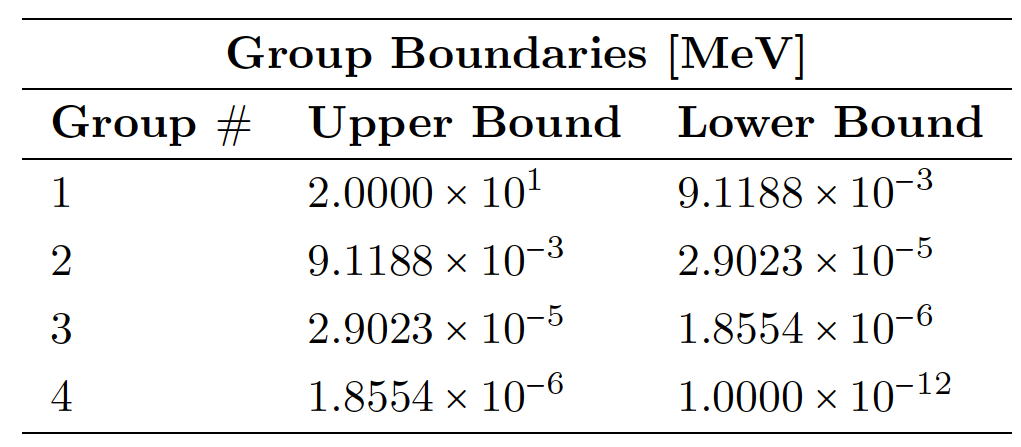
\includegraphics[width=0.6\linewidth]{figures/ahtr-energy-discr.png}
        \end{table}
\end{frame}

\begin{frame}
    \frametitle{AHTR Temperature Model Spatial Homogenization}
        \textbf{Fuel assembly 61 cell discretization}: inter-assembly FLiBe, 
        Y-shaped graphite structure, control rod slot FLiBe, graphite spacers, 
        each diamond shape section's inter-plank FLiBe (3), each graphite plank (18), 
        and each fuel stripe (36)
    \begin{figure}[]
            \centering
            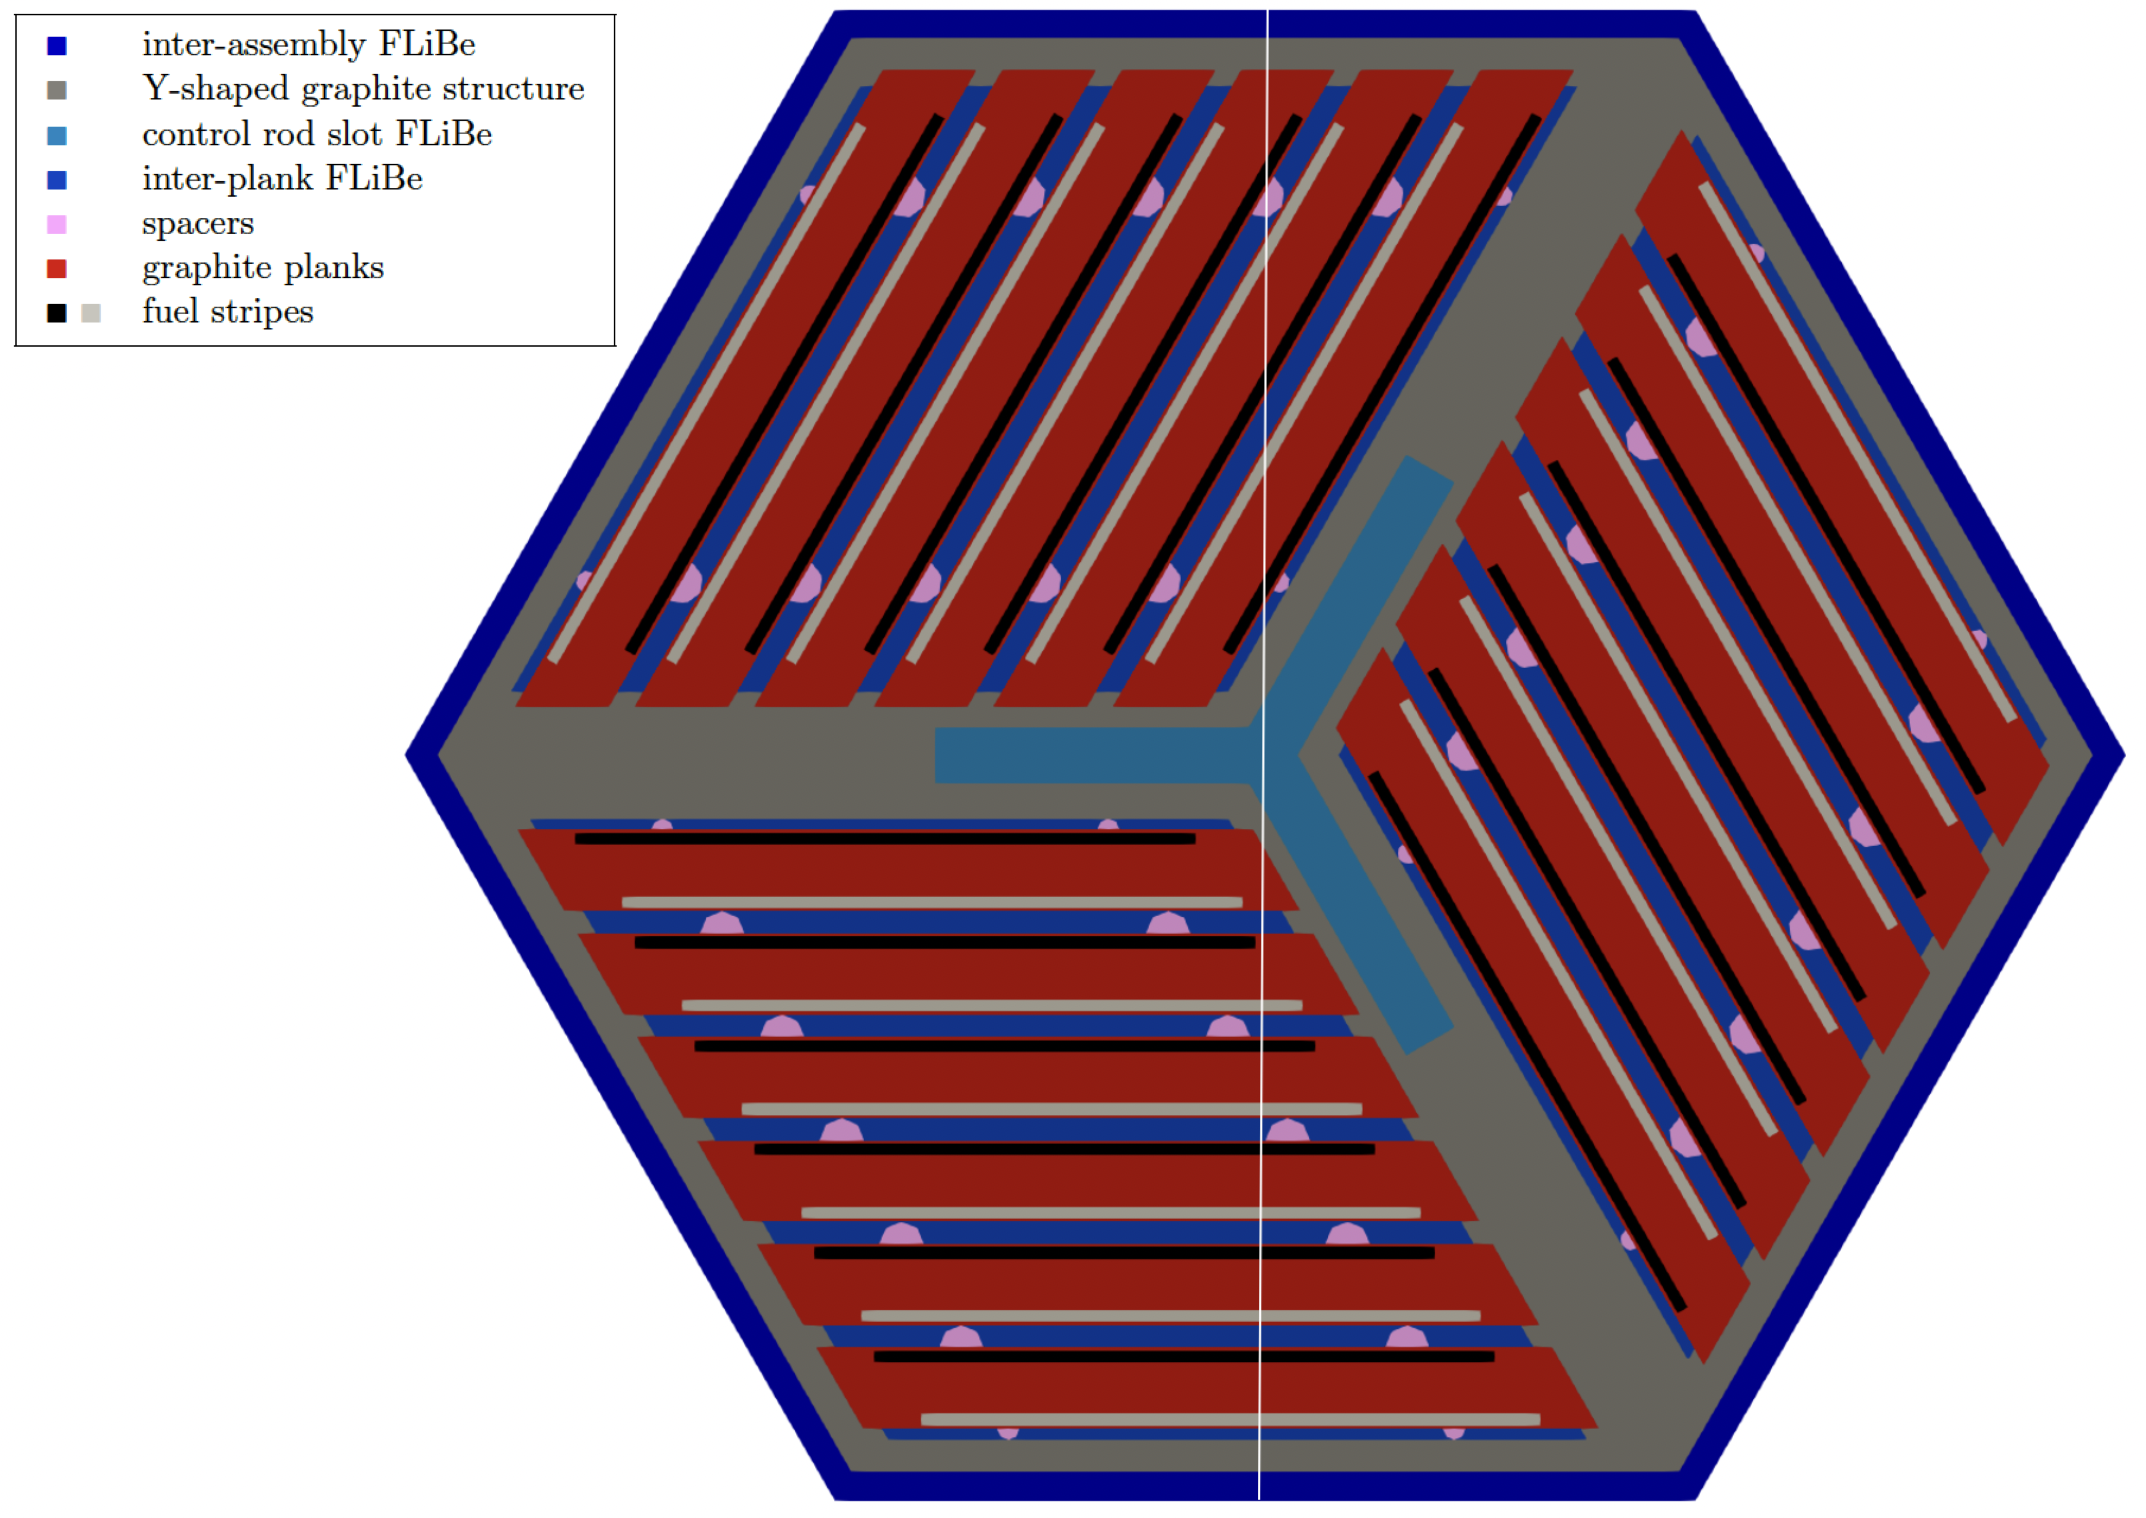
\includegraphics[width=0.65\linewidth]{figures/assembly_mg_pres.png}
        \caption{AHTR assembly spatial homogenization for group constant generation.}
    \end{figure}
\end{frame}

\subsection{Key Neutronics Parameters Verification}
\begin{frame}
    \frametitle{AHTR Temp Model Key Neutronics Parameter Verification}
    I \textbf{verify acceptable spatial homogenization and energy discretization} by 
    comparing key neutronics parameters (KNPs) between: 
    \begin{itemize} 
        \item OpenMC simulation with continuous energy and TRISO-level spatial fidelity
        \item Moltres simulation with 4-group energy and spatial homogenization
    \end{itemize}
    \textbf{KNPs}: $k_{eff}$, reactivity coefficients, flux distribution, and neutron 
    spectrum
    \begin{itemize}
        \item All comparisons are to verify that the Moltres model is replicating the 
        OpenMC model's neutronics correctly
    \end{itemize}
    \textbf{Reactivity coefficients and flux distribution}
    \begin{itemize}
        \item Ensure that \textbf{Moltres accurately calculates the AHTR's temperature 
        distribution}
        \item Reactivity coefficients capture temperature reactivity feedback on the flux
        \item Moltres source term is dependent on flux 
    \end{itemize}
\end{frame}

\begin{frame}
    \frametitle{Key Neutronics Parameter Verification Summary}
    OpenMC vs Moltres models \textbf{key observations} 
    \begin{itemize}
        \item 216 pcm reactivity difference  
        \item Good agreement in reactivity coefficients and 4-group neutron spectrum
        \item Good agreement in overall flux but larger flux diffs at specific points
    \end{itemize}
    Explanations: 
    \begin{itemize}
        \item Reactivity and flux differences due to Moltres' \textbf{neutron diffusion 
        method} 
        \item Differences in reactivity and flux at specific points might result in 
        \textbf{slightly inaccurate temperatures at certain points}
        \item Since the reactivity coefficients and overall flux distribution 
        are in agreement, this spatial homogenization and energy discretization are 
        \textbf{sufficiently accurate} to calculate and gain an \textbf{overall perspective} 
        of the AHTR's temperature distribution
    \end{itemize}
    Methodology 
    \begin{itemize}
        \item I use this same Moltres model verification method for the AHTR geometries 
        used for optimization 
    \end{itemize}
\end{frame}

\subsection{AHTR Temperature Model Results}
\begin{frame}
    \frametitle{AHTR Temperature Model Results}
    \begin{columns}
        \begin{column}{0.6\textwidth}
            \begin{figure}[]
                \centering
                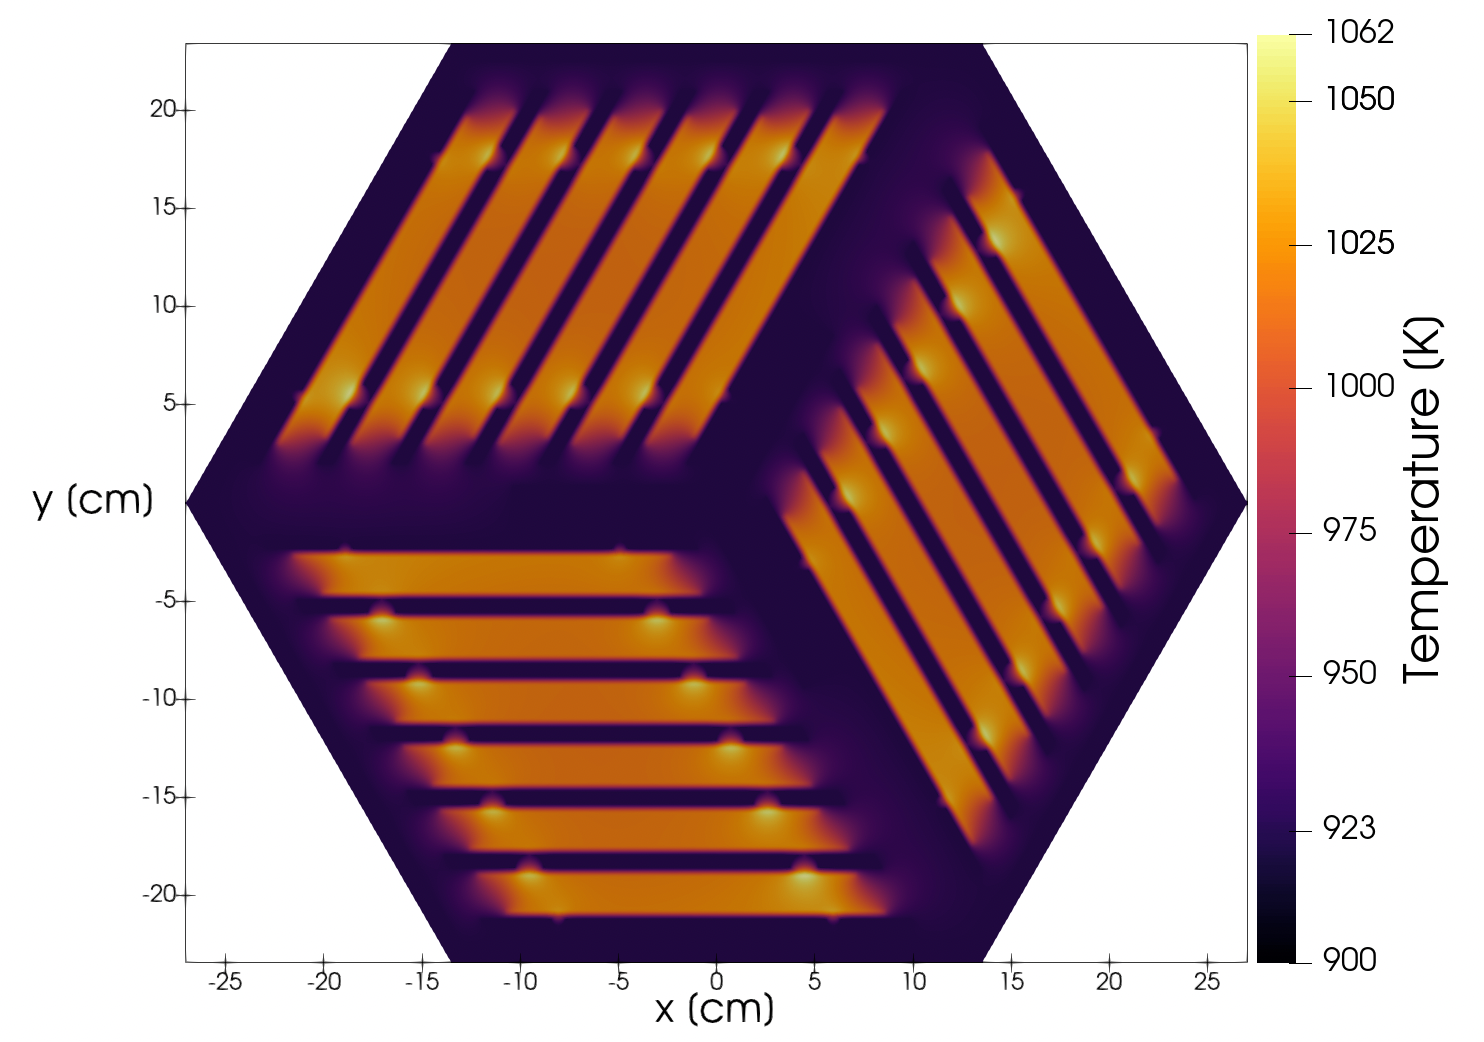
\includegraphics[width=\linewidth]{../docs/figures/benchmark-temperature-model.png} 
                \caption{2D temperature distribution in the \acrfull{AHTR}
                full assembly generated by Moltres.}
            \end{figure}
        \end{column}
        \begin{column}{0.4\textwidth} 
            \begin{block}{Results}
                \begin{itemize}
                    \item Average temperature distribution across the fuel planks are 
                    $\approx 1025K$
                    \item Average temperature of graphite structure is $\approx 935K$
                    \item Temperature peaks at 1062K in the fuel stripes near the spacers
                    \item This is due to the spacers displacing coolant and providing extra 
                    moderation 
                \end{itemize}
            \end{block}
        \end{column}
        \end{columns}
\end{frame}

\subsection{Summary}
\begin{frame}
    \frametitle{FHR Benchmark + AHTR Temperature Model: Summary}
    \begin{block}{I Successfully Completed AHTR Model Development Research Objectives}
        \begin{itemize}
            \item I participated in the OECD-NEA's FHR Benchmark Phases I-A and I-B
            \item I modeled the \gls{AHTR}'s temperature distribution with Moltres
        \end{itemize}
    \end{block}
    \begin{block}{Major Takeaways}
        \begin{itemize}
            \item AHTR has passive safety behavior with negative temperature coeffcients
            \item Increased fuel packing does not always correspond with increased 
            $k_{eff}$ due to self-shielding effects 
            \item These results hint at the possibility of \textbf{minimizing fuel required by 
            optimizing for heterogenous fuel distributions} within the core
            \item AHTR temperature peaks in the fuel stripes near the spacers 
        \end{itemize}
    \end{block}
\end{frame}


\section{AHTR Optimization for Non-Conventional Designs}
\subsection{Optimization Methodology}
\begin{frame}
    \frametitle{AHTR Optimization Problem Definitions}
    \vspace{-0.2cm}
    \visible<1->{\begin{block}{Varied Input Parameters}
        \begin{itemize}
            \item Total fuel packing fraction ($PF_{total}$)
            \item TRISO fuel packing fraction distribution ($\rho_{TRISO}(\vec{r})$)
            \item Coolant channel shape ($r_i$)
        \end{itemize}}
        \visible<2->{Varying $PF_{total}$ and $\rho_{TRISO}(\vec{r})$ synergistically 
        explores how \textbf{heterogenous TRISO distribution could minimize 
        self-shielding} and thus, reduce the fuel required.}
    \end{block}
    \vspace{-0.3cm}
    \visible<3->{\begin{block}{AHTR Optimization Objectives}
     \textbf{Minimize total fuel packing fraction ($PF_{total}$)}
     \begin{itemize}
        \item Cost savings, non-proliferation 
     \end{itemize}
     \textbf{Minimize maximum temperature ($T_{max}$)}
     \begin{itemize}
        \item Minimize thermal stress in the fuel 
     \end{itemize}
     \textbf{Minimize fuel-normalized power peaking factor ($PPF_{fuel}$)} 
     \begin{itemize}
        \item Efficient fuel utilization
     \end{itemize}
    \end{block}}
    \visible<4->{\textbf{I optimized the AHTR plank and one-third assembly geometries.}} 
\end{frame}

\begin{frame}
    \frametitle{AHTR One-Third Assembly Geometry}
    \begin{figure}
        \only<1>{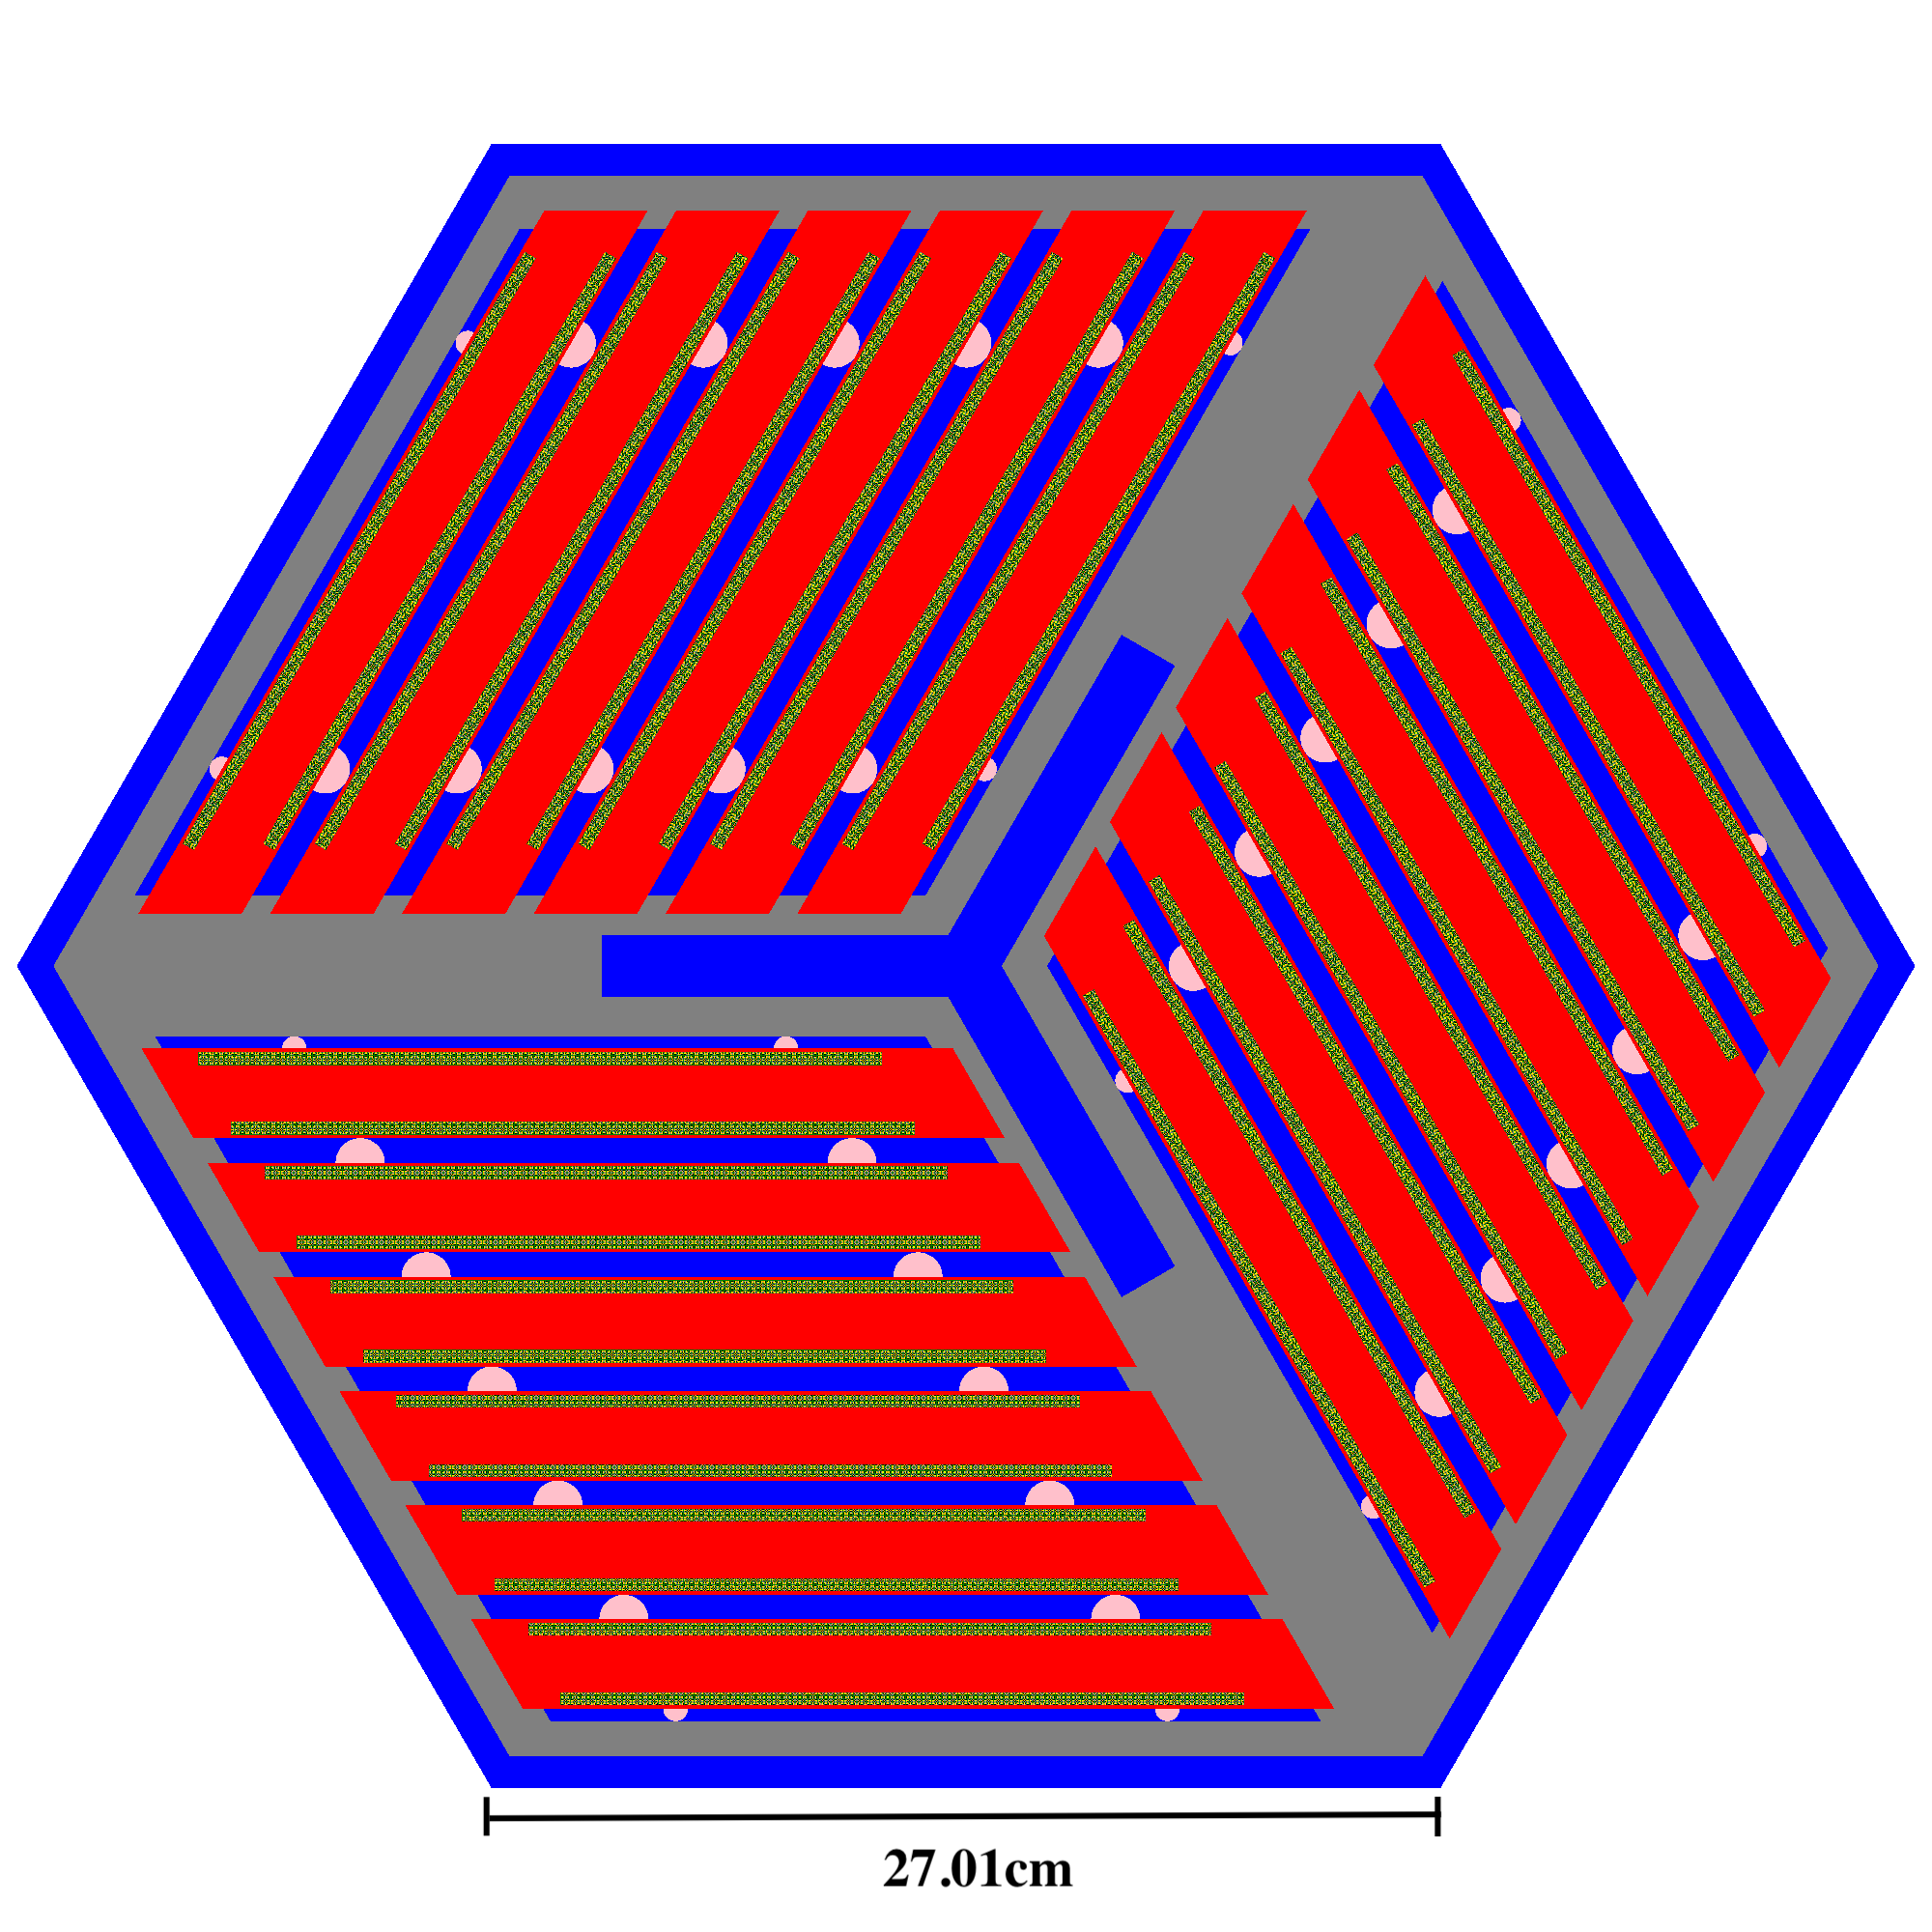
\includegraphics[width=0.6\linewidth]{../docs/figures/ahtr-fuel-element.png}} 
        \only<2>{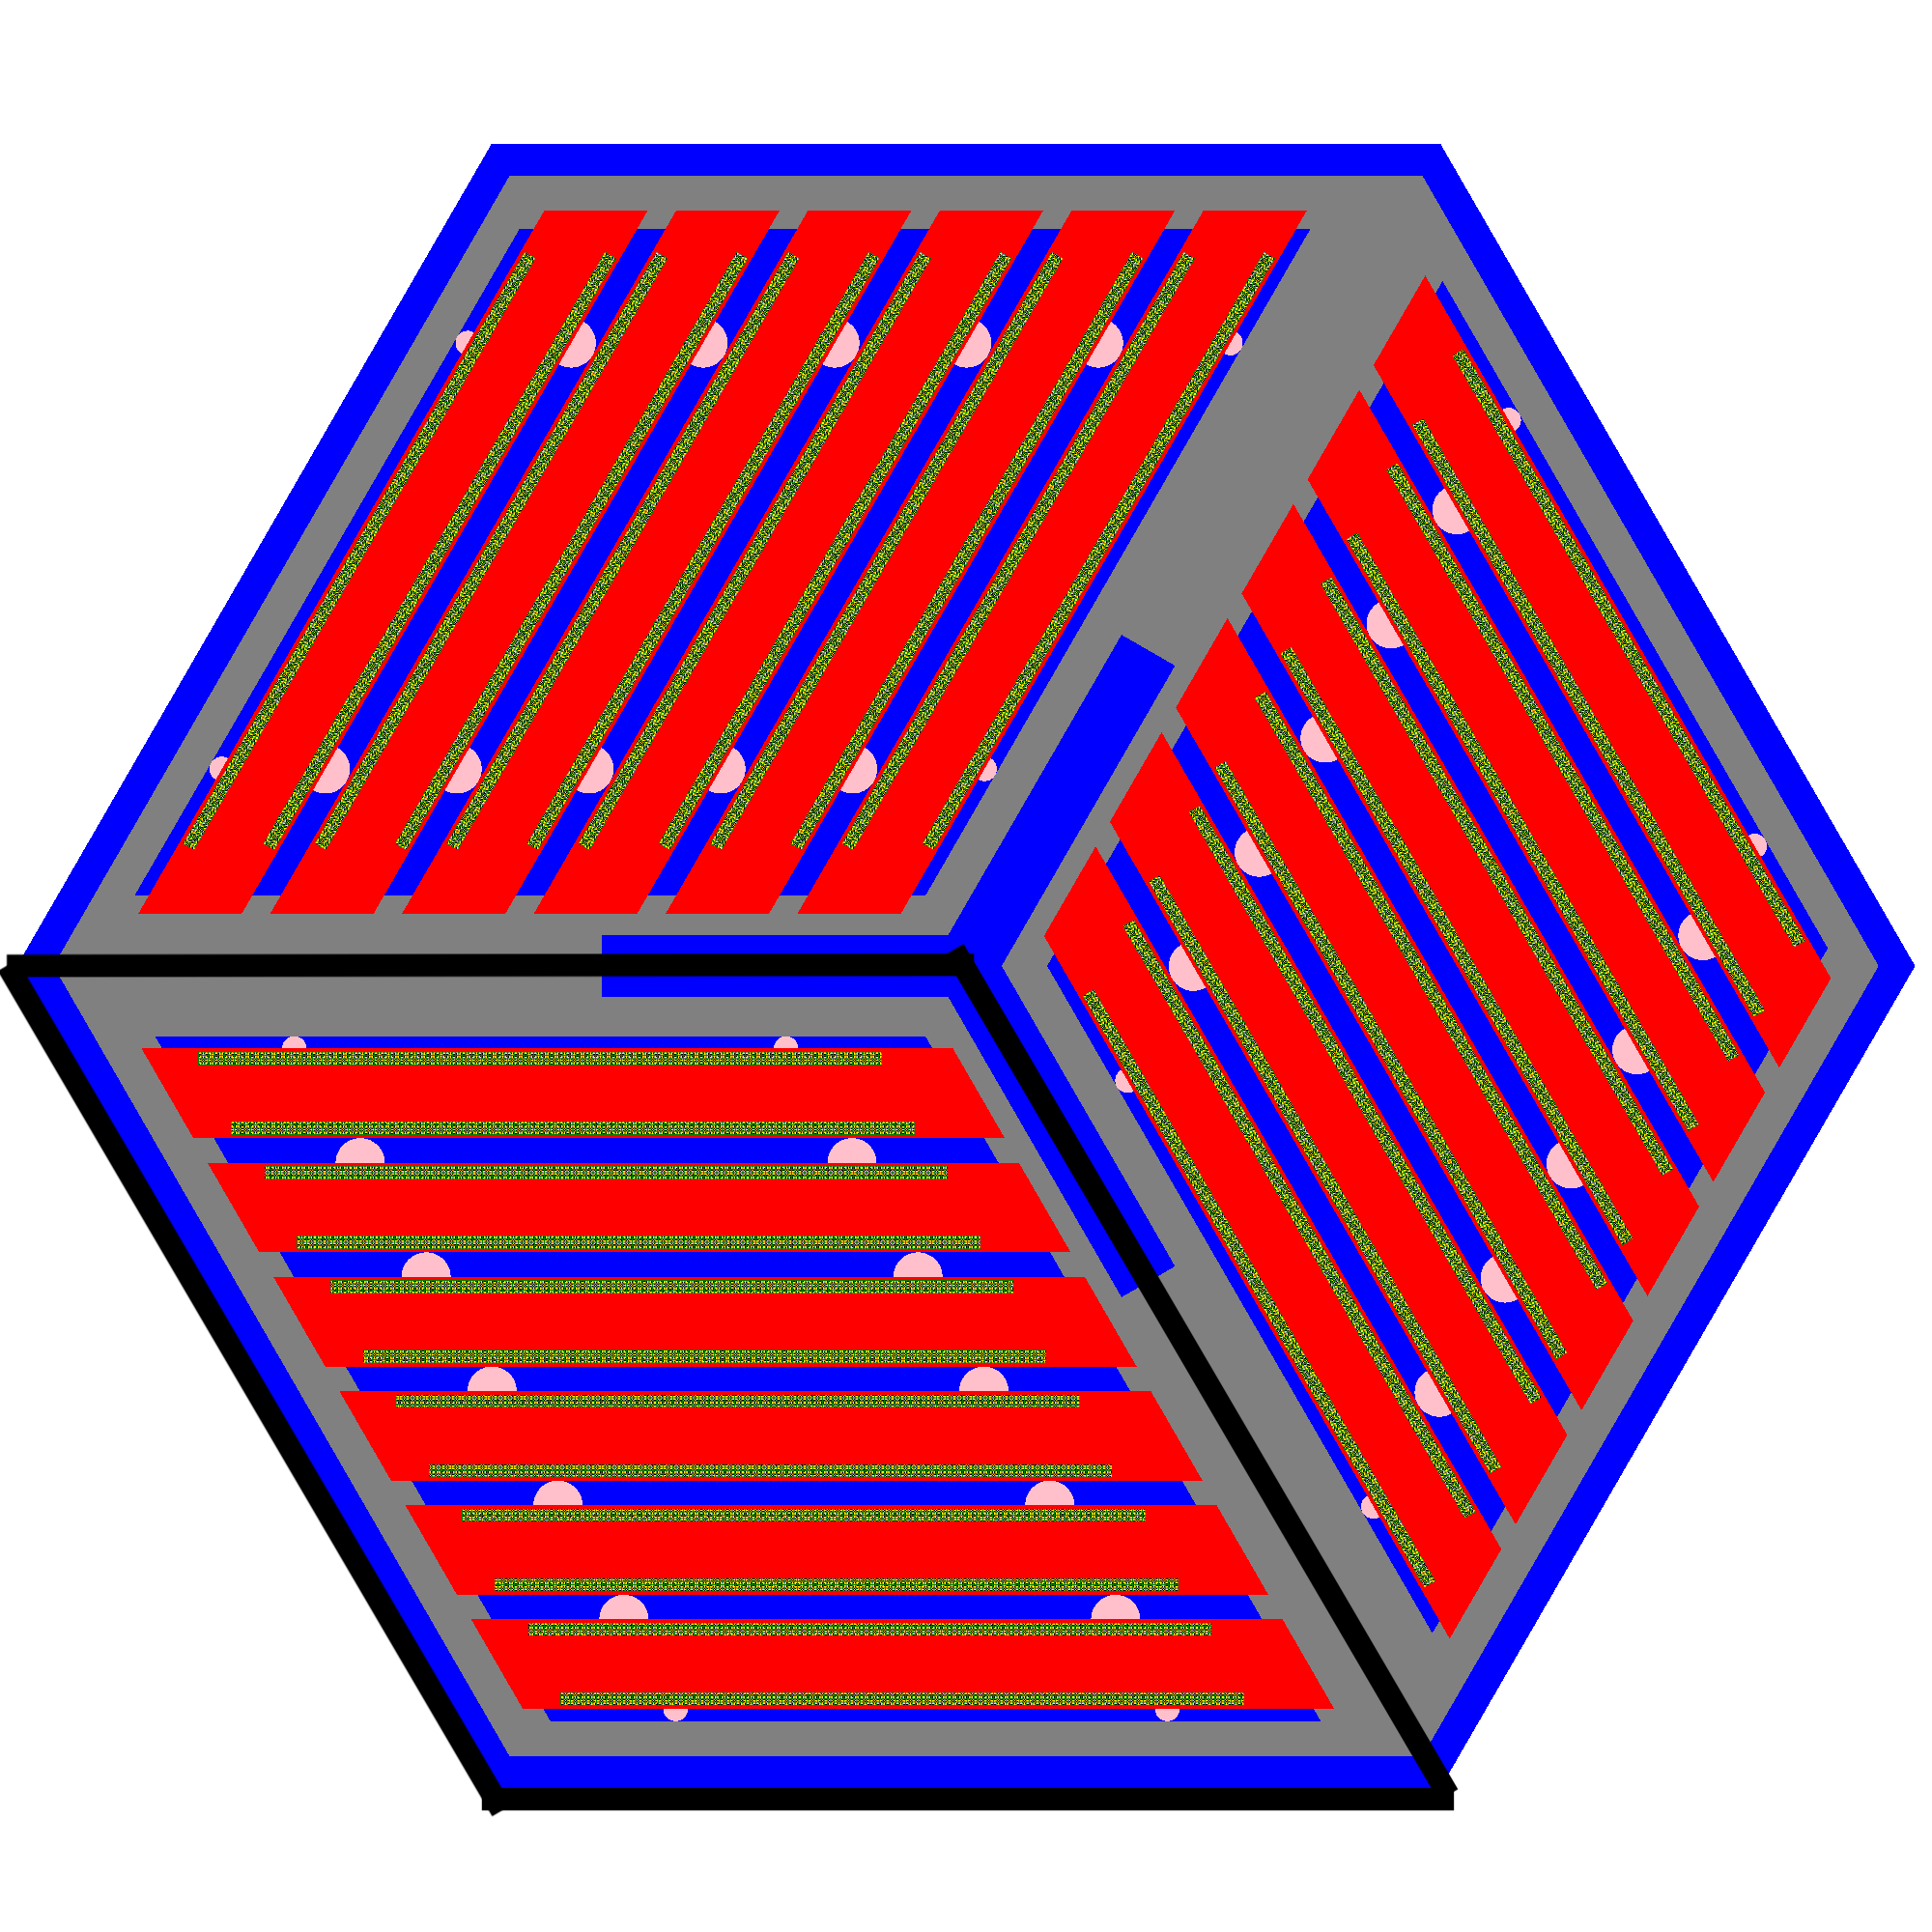
\includegraphics[width=0.6\linewidth]{figures/ahtr-fuel-element-annotated.png}} 
    \end{figure}
\end{frame}

\begin{frame}
    \frametitle{AHTR One-Third Assembly Geometry}
    \visible<1->{\textbf{Two sine distributions govern TRISO packing fraction distribution:}
    \begin{align}
    \rho_{TRISO}(\vec{x}, \vec{y}) &= \left(\textbf{a}\cdot sin(\textbf{b}\cdot 
    x + \textbf{c}) + 2\right) \cdot \left(\textbf{d}\cdot sin(\textbf{e}\cdot y + 
    \textbf{f}) + 2\right) \cdot NF \nonumber
    \end{align}
    
    The normalization factor (NF) ensures that total amount of TRISO particles in the 
    one-third assembly corresponds to $PF_{total}$.}

    \vspace{-0.3cm}
    \begin{columns}[t]
        \begin{column}{0.5\textwidth}
        \begin{figure}
            \only<1-2>{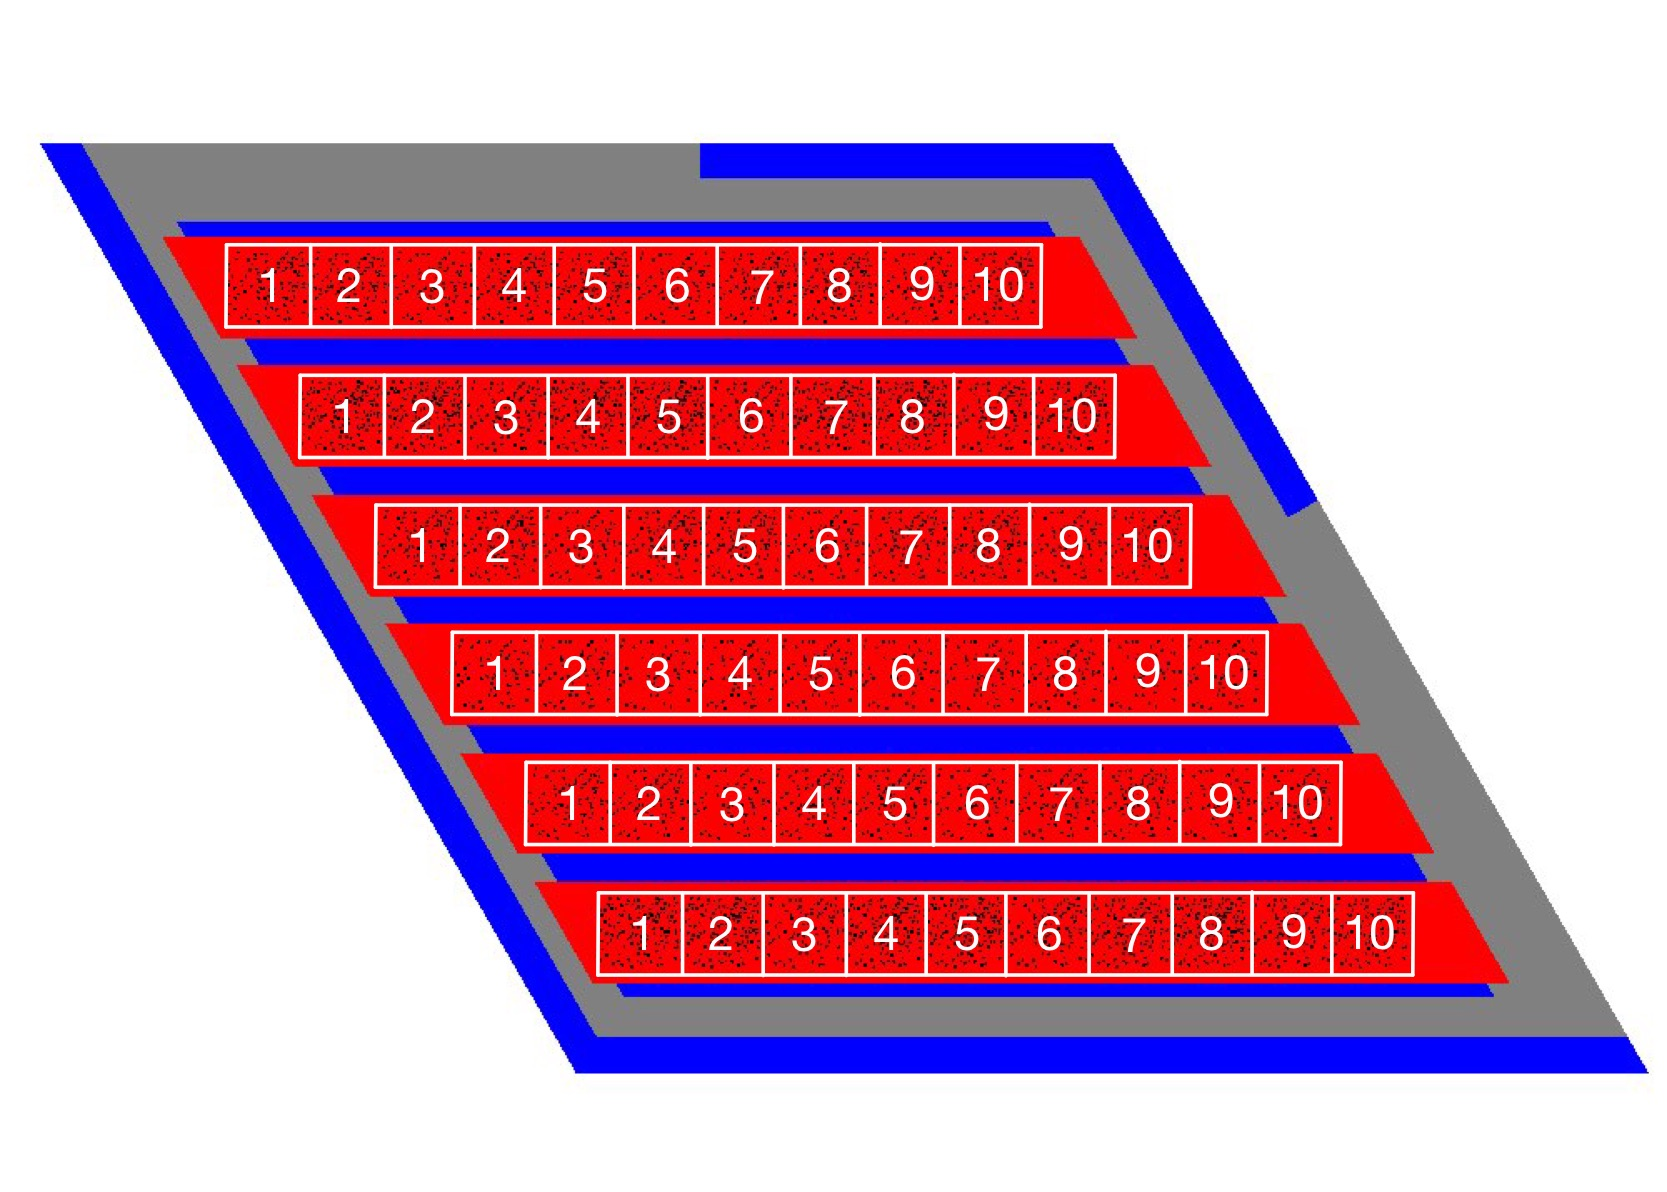
\includegraphics[width=\linewidth]{../docs/figures/ahtr_assembly.png} 
            \vspace{-0.6cm}
            \caption{AHTR one-third assembly illustrating packing fraction discretization.}}
            \only<3>{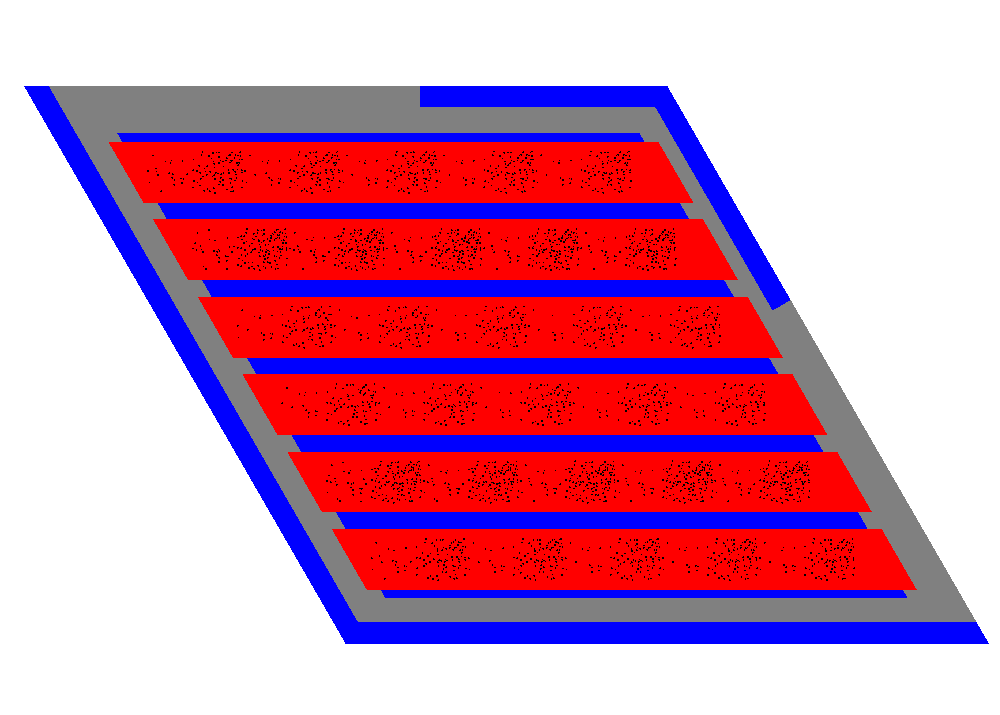
\includegraphics[width=\linewidth]{../docs/figures/assem-obj-1-pf-most-minimized.png} 
            \vspace{-0.6cm}
            \caption{AHTR one-third assembly illustrating packing fraction variation.}}
        \end{figure}
        \end{column}
        \begin{column}{0.5\textwidth} 
            \visible<2->{\begin{figure}
                \textbf{a} = 1.435, \textbf{b} = 1.488, \textbf{c} = 2.362, \\
                \textbf{d} = 0.689, \textbf{e} = 0.584, \textbf{f} = 4.170
                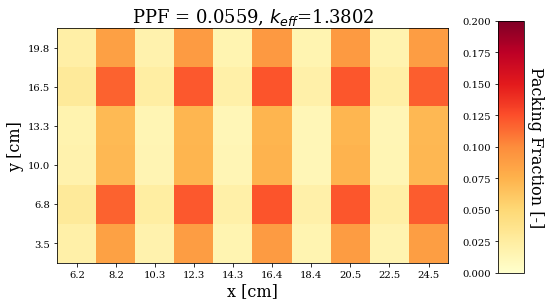
\includegraphics[width=\linewidth]{../docs/figures/assem-0.0559-most-minimized.png} 
                \caption{TRISO distribution example.}
            \end{figure}}
        \end{column}
        \end{columns}
\end{frame}

\begin{frame}
    \frametitle{Contd. AHTR One-Third Assembly Geometry}
    \textbf{Five radius values (\textbf{$r_1, r_2, r_3, r_4, r_5$}) 
    control coolant channel shape.}
    \begin{figure}
        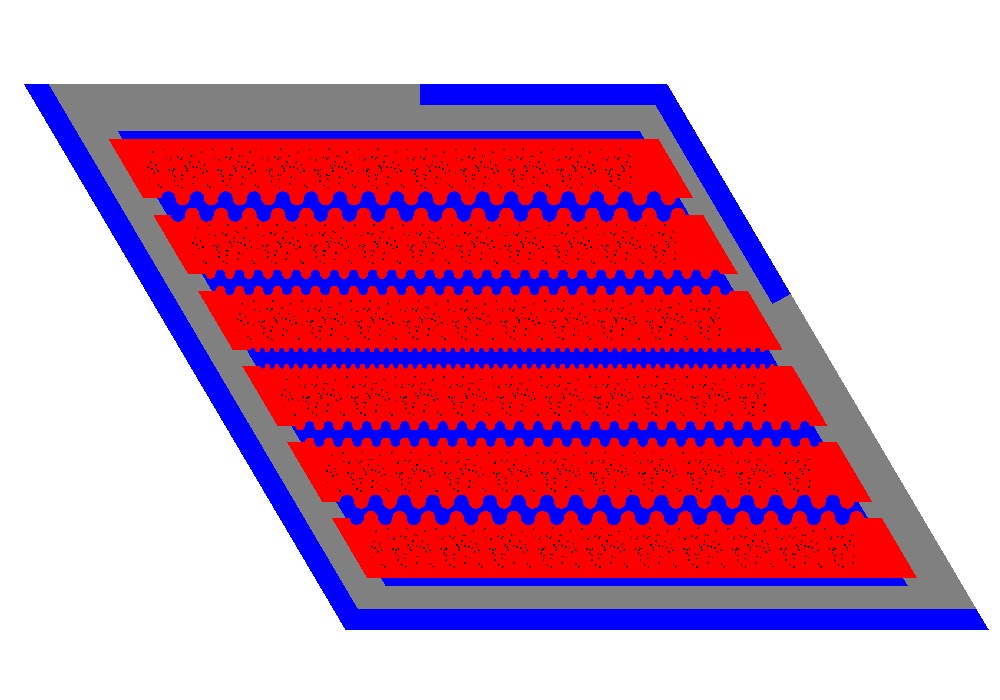
\includegraphics[width=0.7\linewidth]{../docs/figures/coolant-channel-shape-assem.png} 
        \vspace{-0.3cm}
        \caption{AHTR one-third assembly with coolant channel shape variation, 
        $r_1, r_2, r_3, r_4, r_5$ = 0.3cm, 0.2cm, 0.1cm, 0.2cm, 0.3cm.}
    \end{figure}
\end{frame}

\begin{frame}
    \frametitle{ROLLO AHTR Optimization Workflow}
    \vspace{-0.2cm}
    \begin{figure}
        \makebox[\textwidth][c]{
            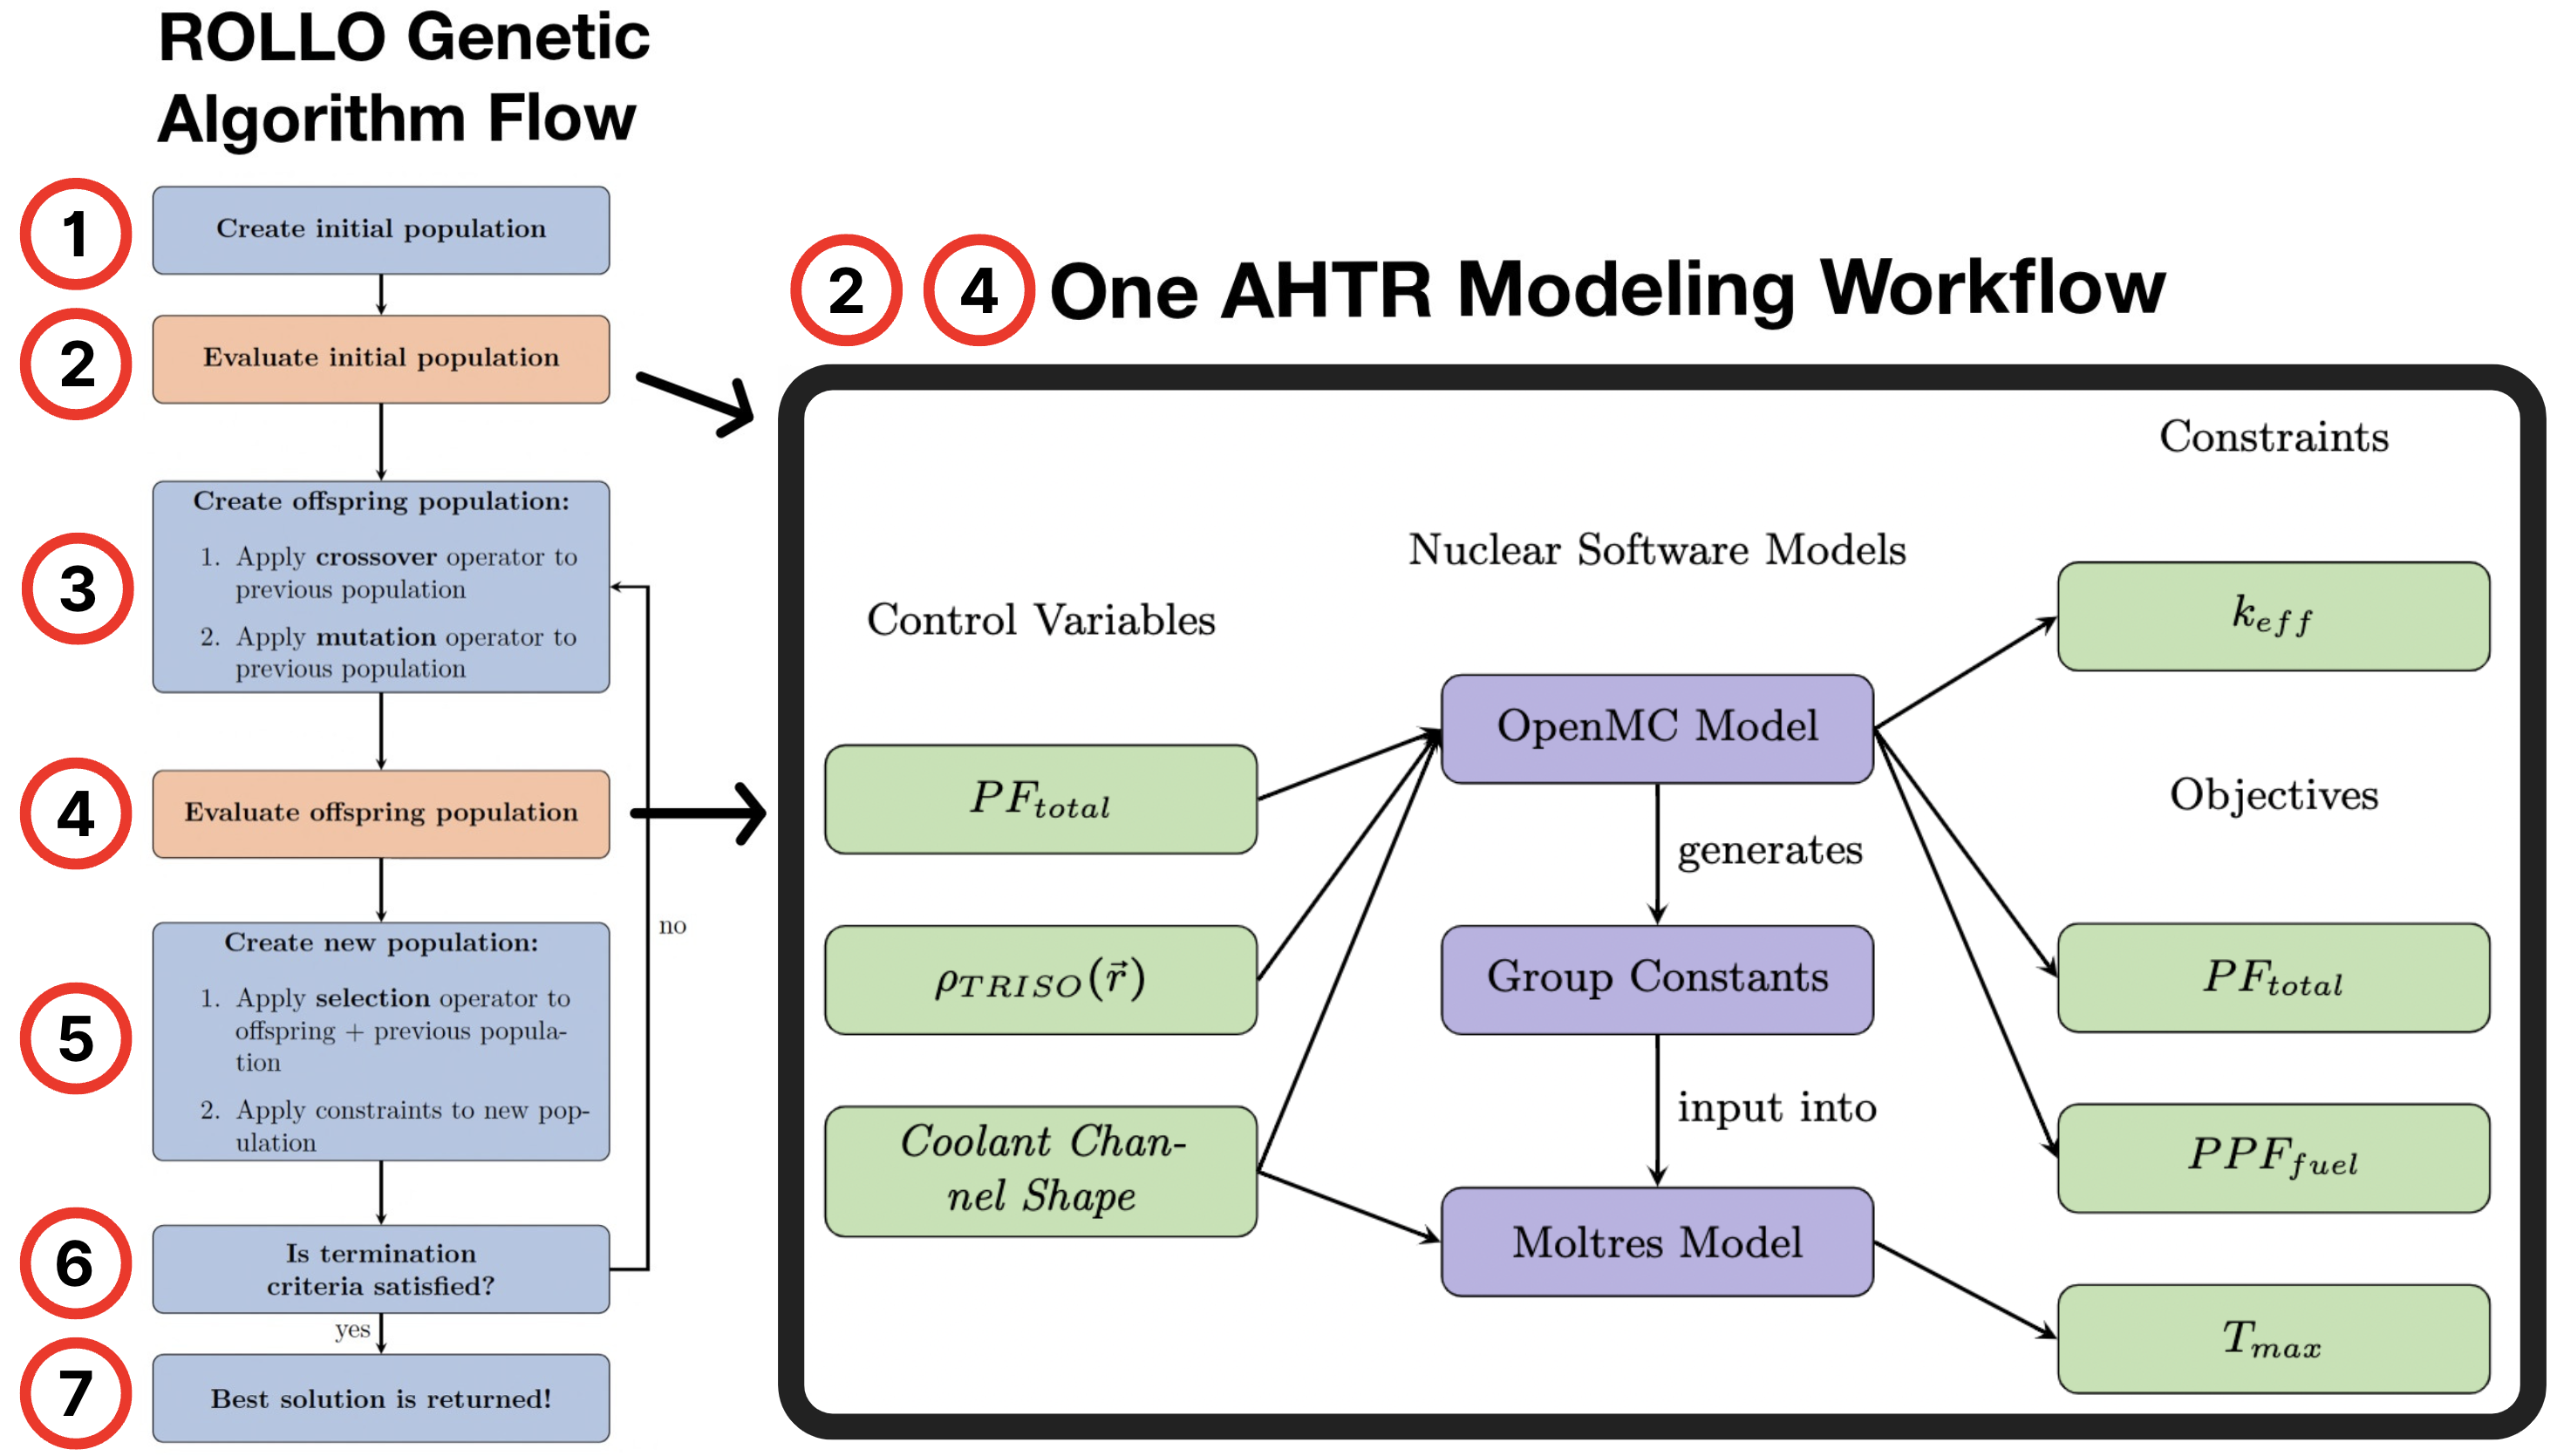
\includegraphics[width=1.1\linewidth]{figures/ahtr-modeling-workflow-numbered.png}} 
        %\caption{ROLLO AHTR Optimization Workflow.}
    \end{figure}
\end{frame}

\subsection{AHTR One-Third Assembly Optimization Results}
\begin{frame}
    \frametitle{AHTR One-Third Assembly Optimization Simulations}
    \only<1>{
        \vspace{-0.2cm}
        \begin{figure}
            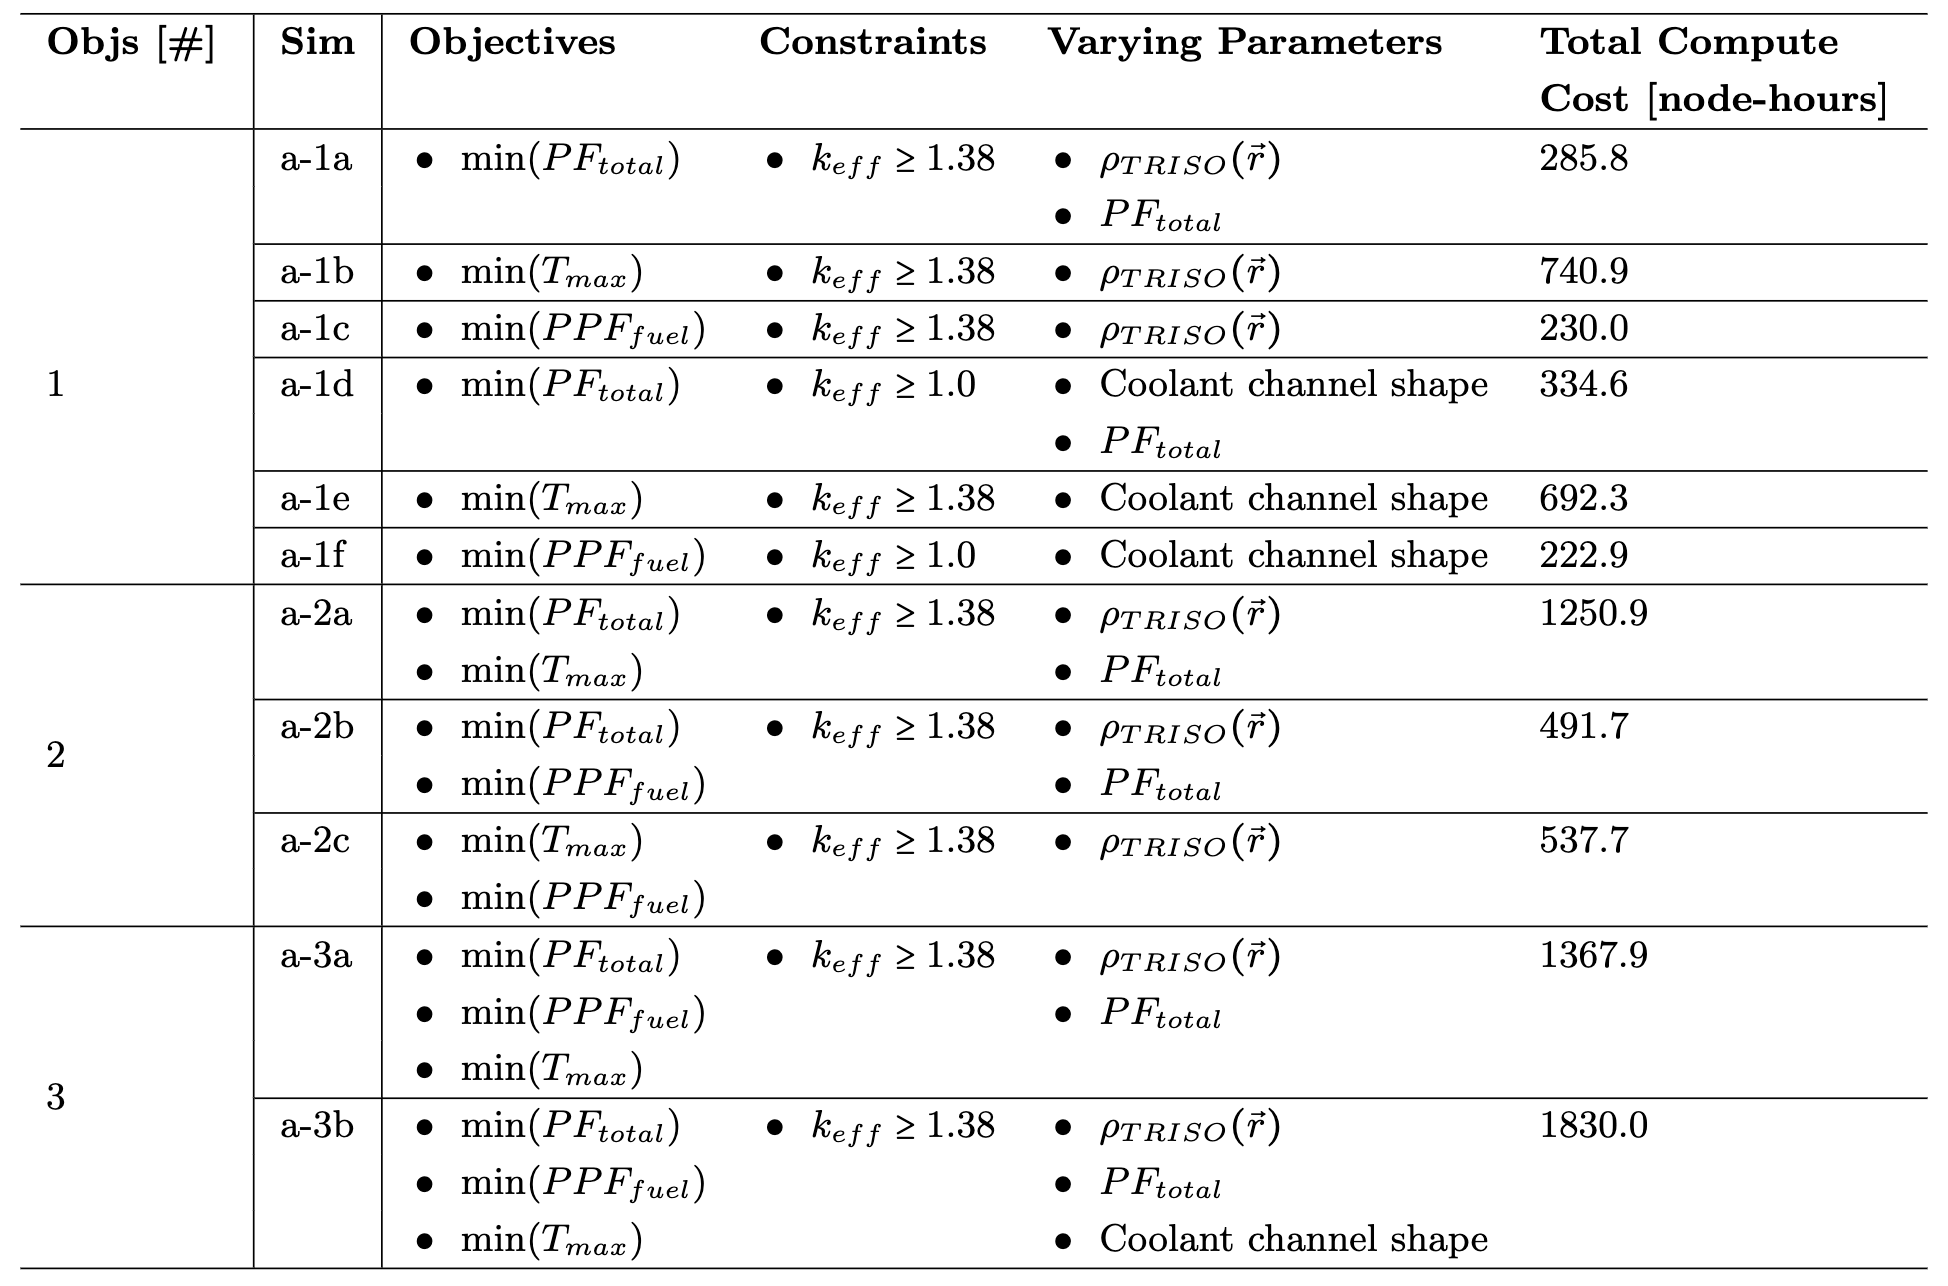
\includegraphics[width=0.8\linewidth]{figures/ahtr-assem-opt-table.png}
        \end{figure}

        \vspace{-0.2cm}
        \textbf{All the optimization simulations are run on the Theta supercomputer} 
        at the Argonne Leadership Computing Facility \cite{noauthor_thetathetagpu_2022}.

        Each Theta node has 64 1.3-GHz Intel Xeon Phi 7230 processors.
        }

        \only<2>{
            \begin{figure}
                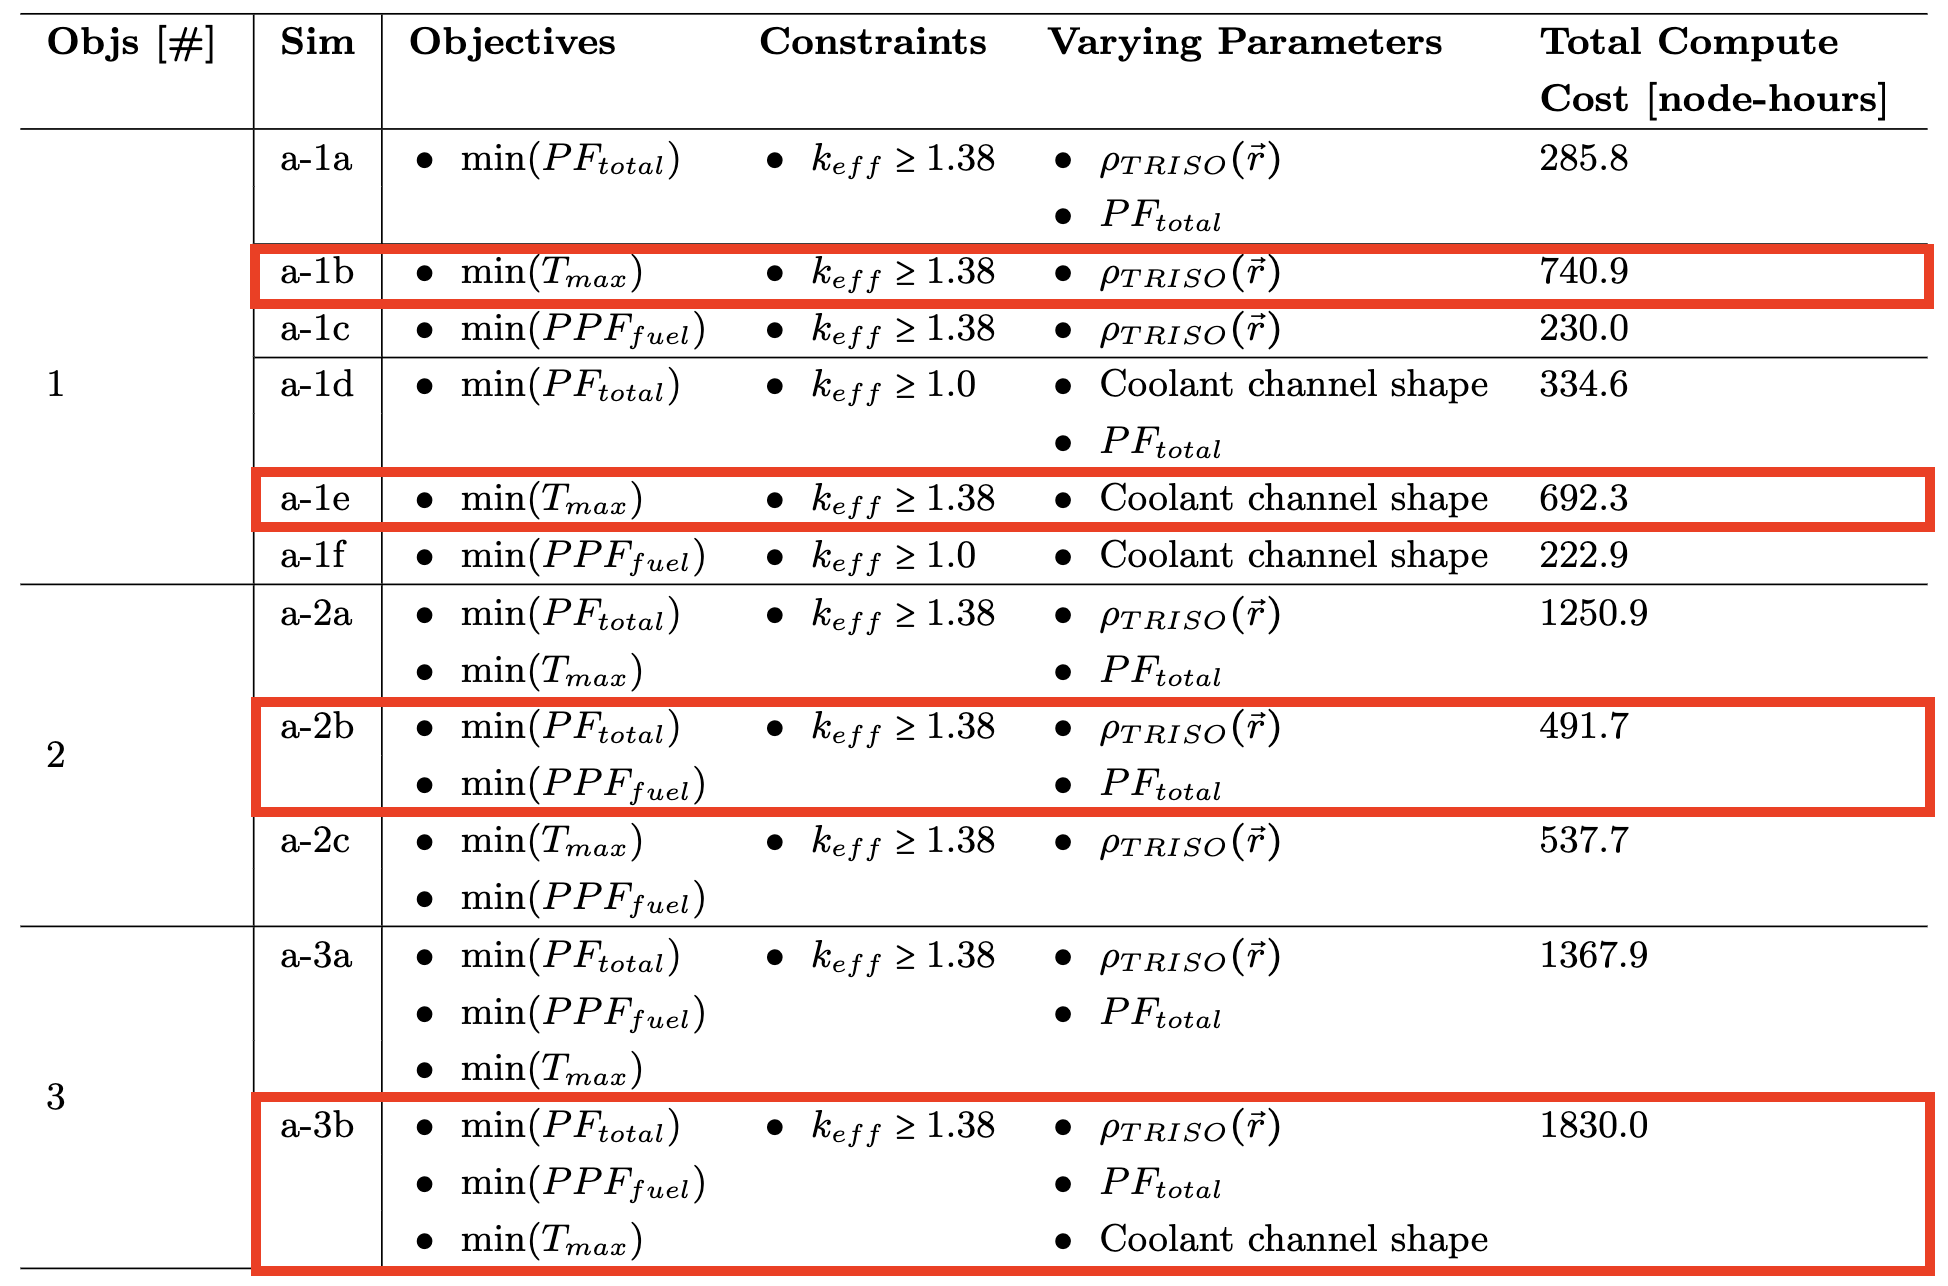
\includegraphics[width=0.9\linewidth]{figures/ahtr-assem-opt-table-annotated.png}
            \end{figure}}

        \only<3>{
            \begin{figure}
                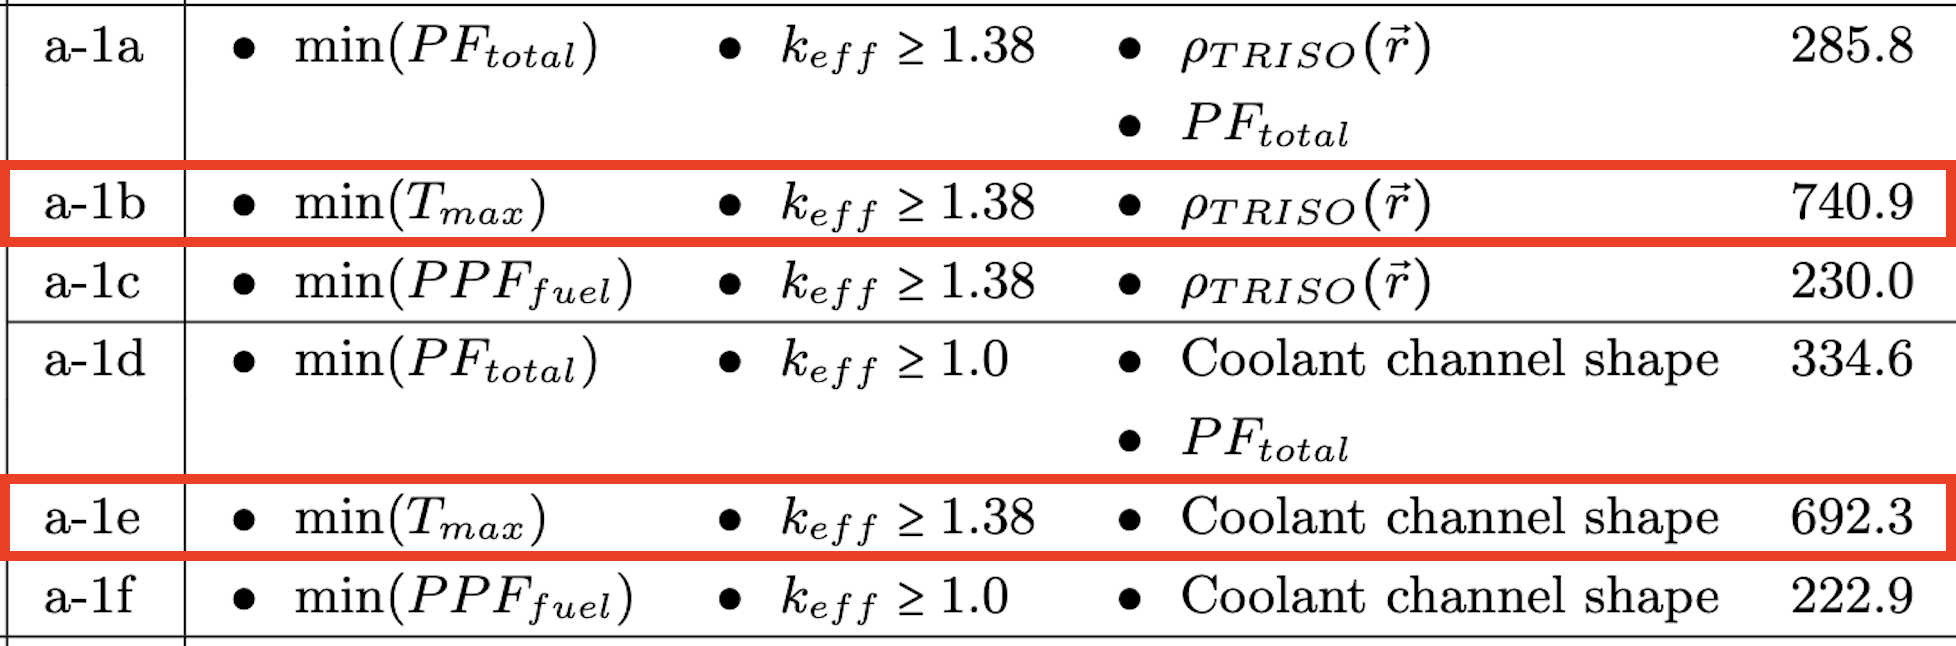
\includegraphics[width=\linewidth]{figures/ahtr-assem-opt-table-annotated1.png}
            \end{figure}
    
            Simulations a-1b and a-1e demonstrate \textbf{how the input parameters 
            $\rho_{TRISO}(\vec{r})$ and coolant channel shape respond to 
            the minimize $T_{max}$ objective}.

            \vspace{0.2cm}
            I constrained $k_{eff} \geq 1.38$ find optimal input parameters 
            that achieve \textbf{similar performance to the FHR benchmark} TRISO distribution.}
        
        \only<4>{
            \begin{figure}
                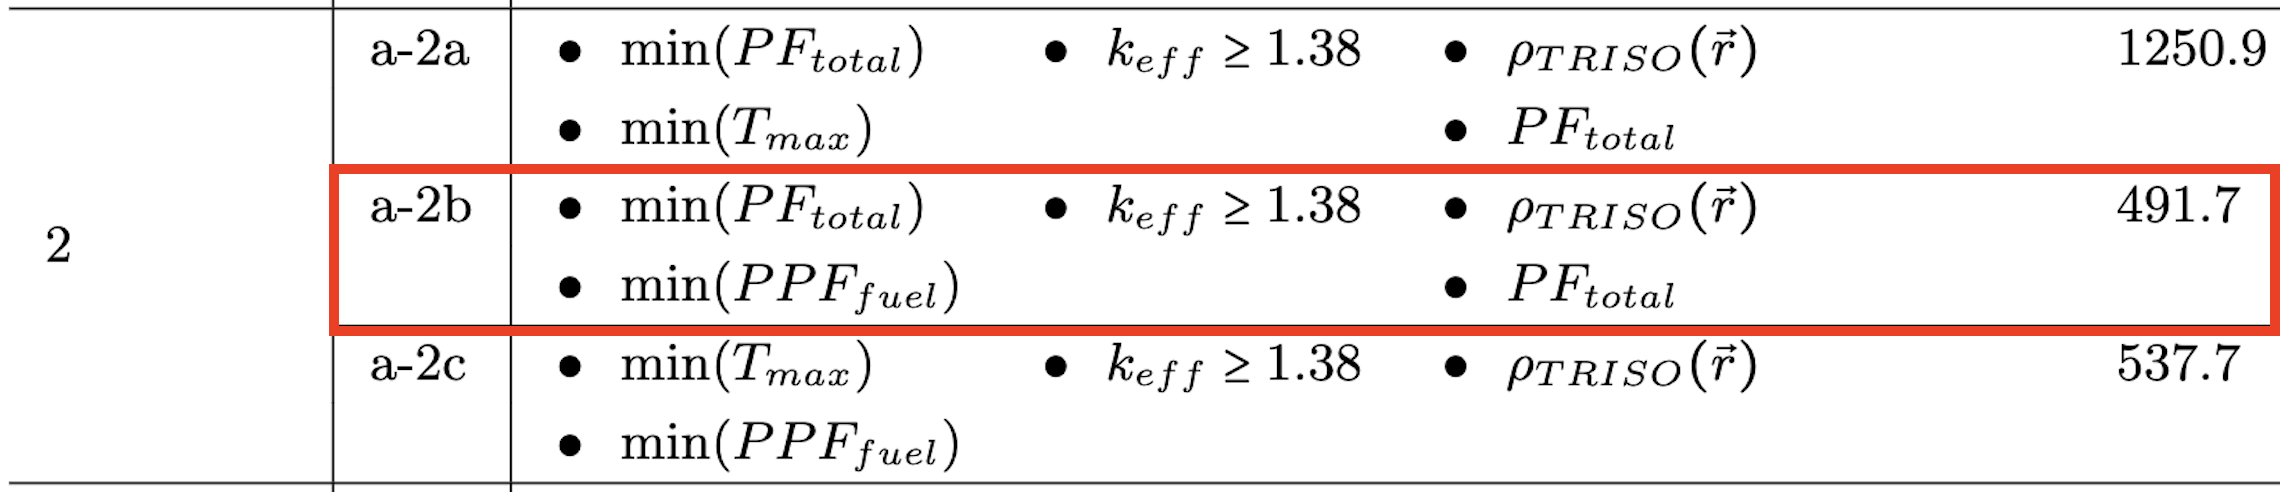
\includegraphics[width=\linewidth]{figures/ahtr-assem-opt-table-annotated2.png}
            \end{figure}

            Simulation a-2b demonstrates \textbf{how the input parameters $PF_{total}$ 
            and $\rho_{TRISO}(\vec{r})$ change as the minimize $PF_{total}$ and 
            $PPF_{fuel}$ objectives interact}.
        }

        \only<5>{
            \begin{figure}
                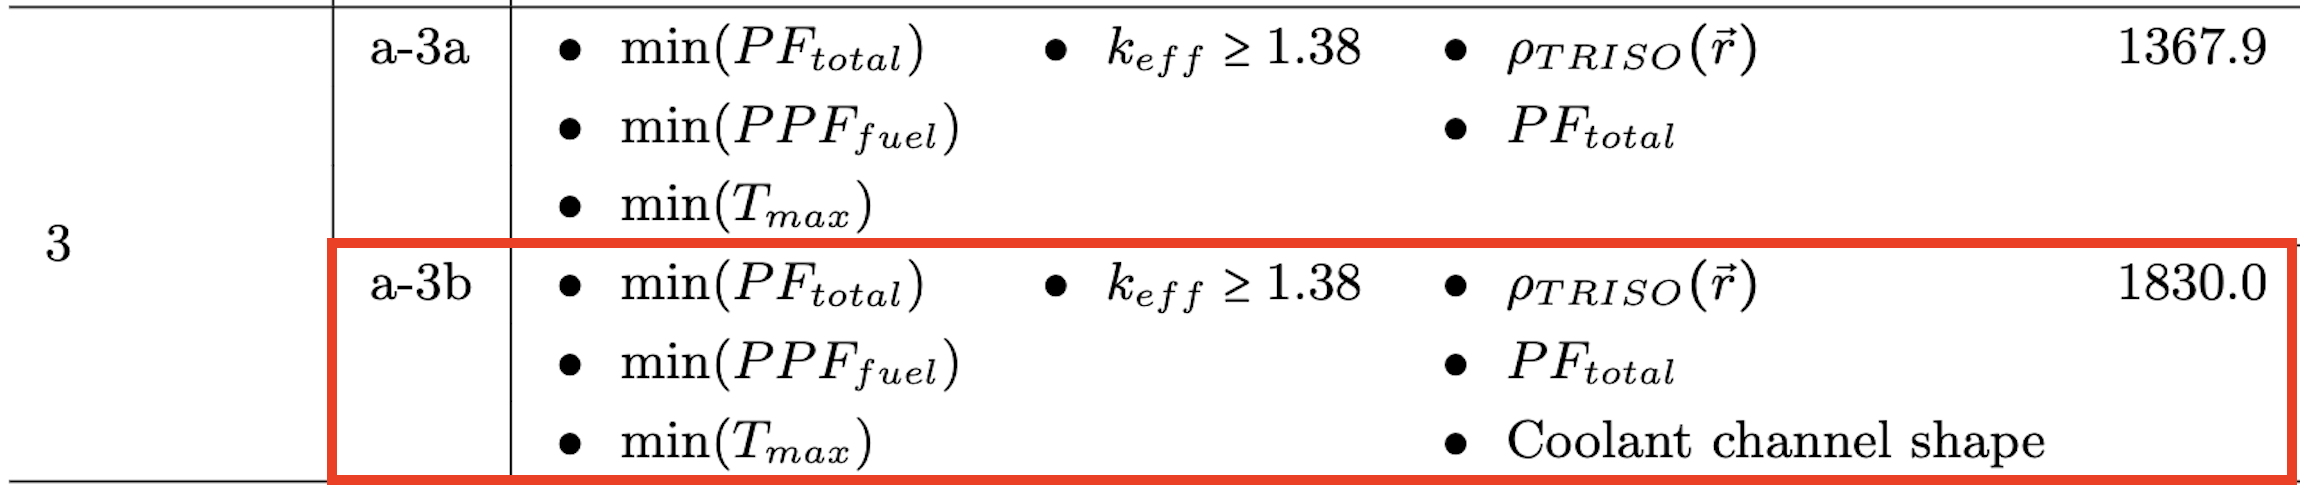
\includegraphics[width=\linewidth]{figures/ahtr-assem-opt-table-annotated3.png}
            \end{figure}

            Simulation a-3b is the \textbf{final and largest optimization problem} run 
            for the one-third assembly model that varies all input parameters to optimize 
            for all objectives. 
        }
    
\end{frame}

\begin{frame}
    \frametitle{AHTR One-Third Assembly Simulation a-1b Results}
    \visible<1->{\textbf{Simulation a-1b: I vary a, b, c, d, e f ($\rho_{TRISO}(\vec{x}, \vec{y})$)
    to minimize $T_{max}$.}} 

    \begin{figure}
        \only<1,4>{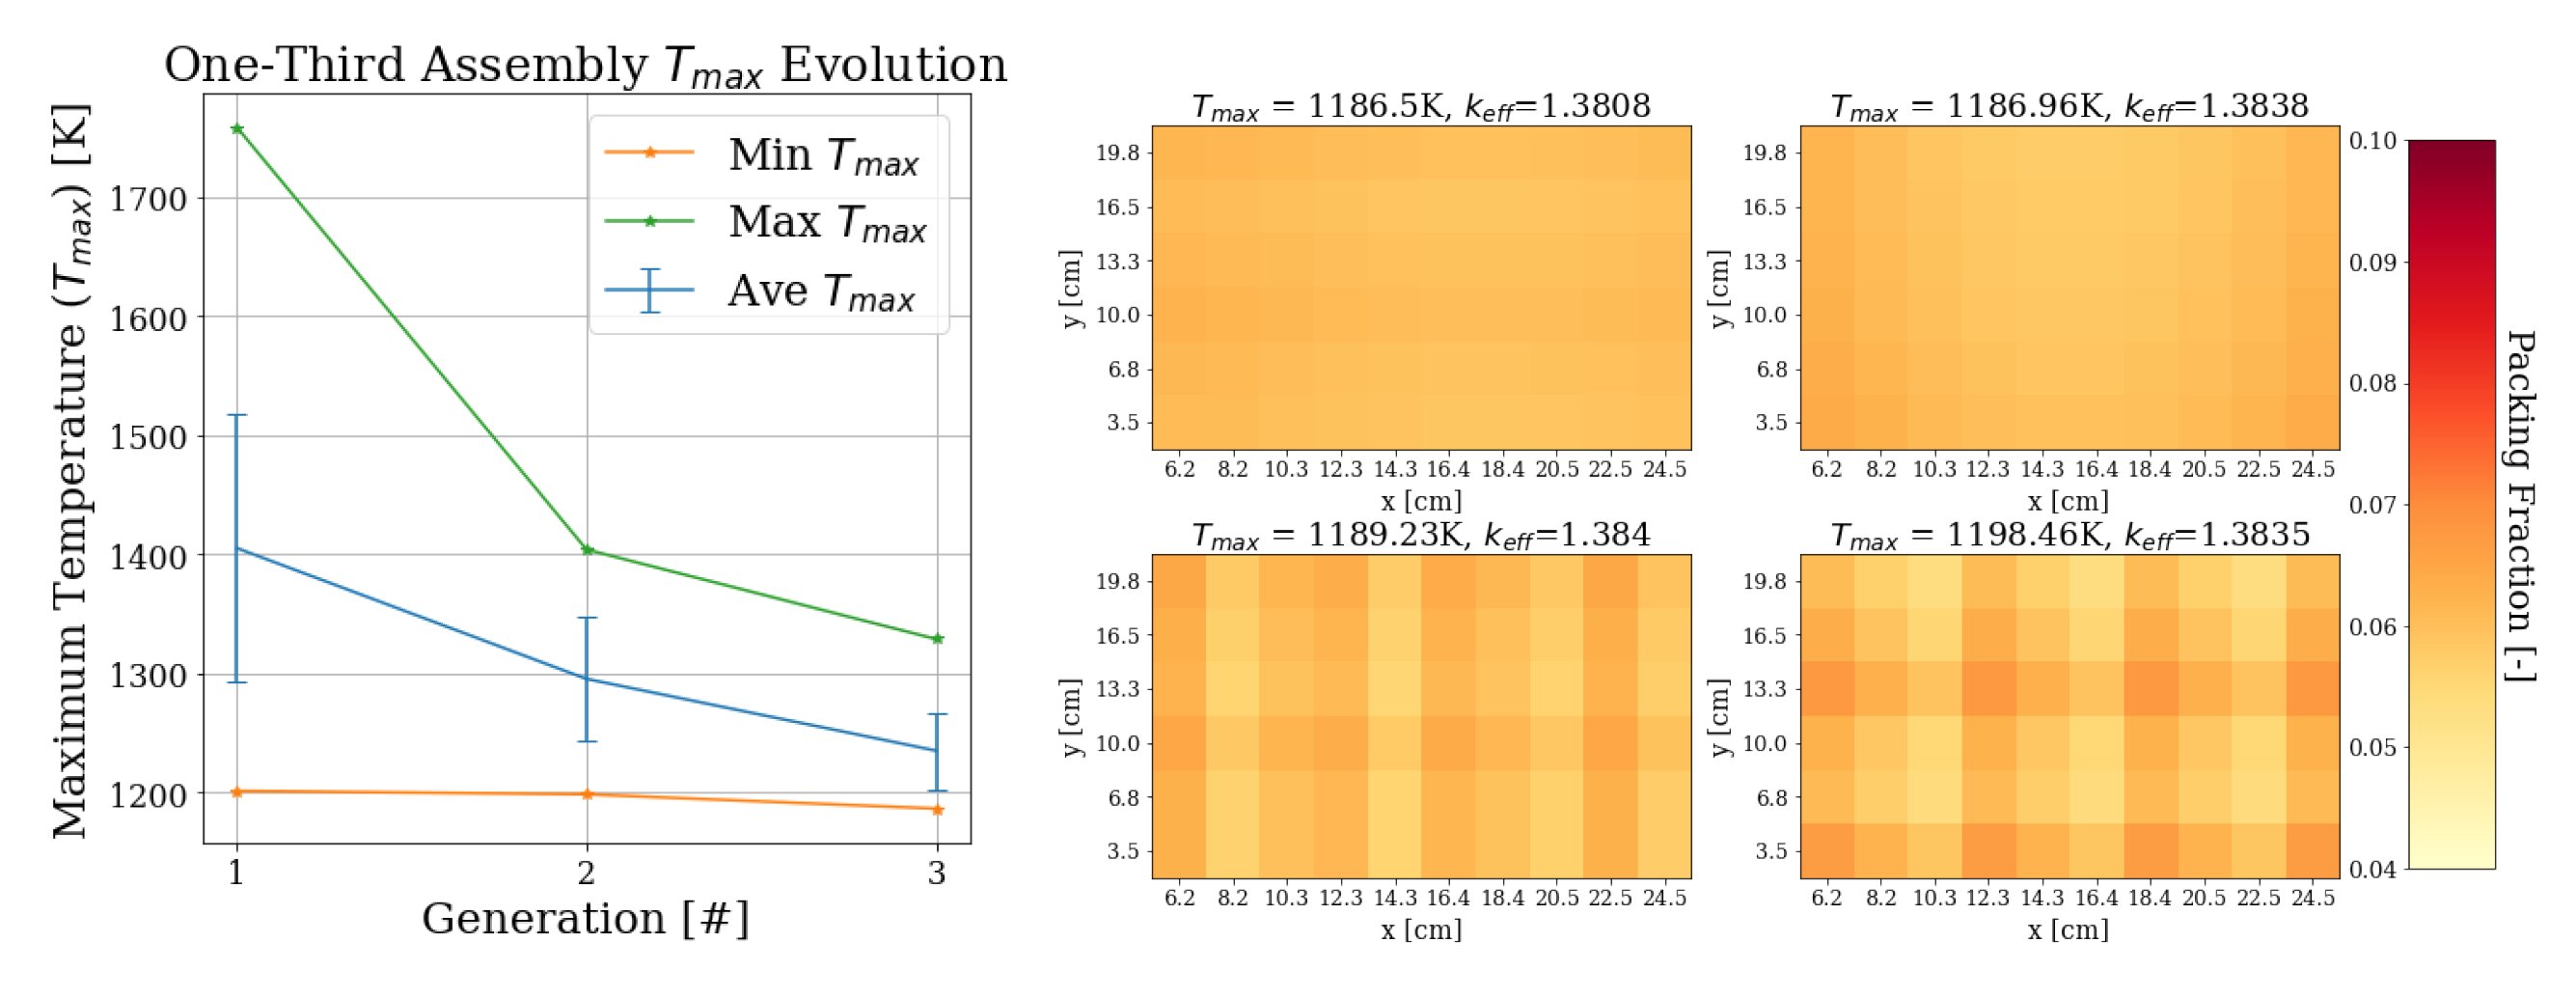
\includegraphics[width=\linewidth]{figures/assem-obj-1-temp.png}}
        \only<2>{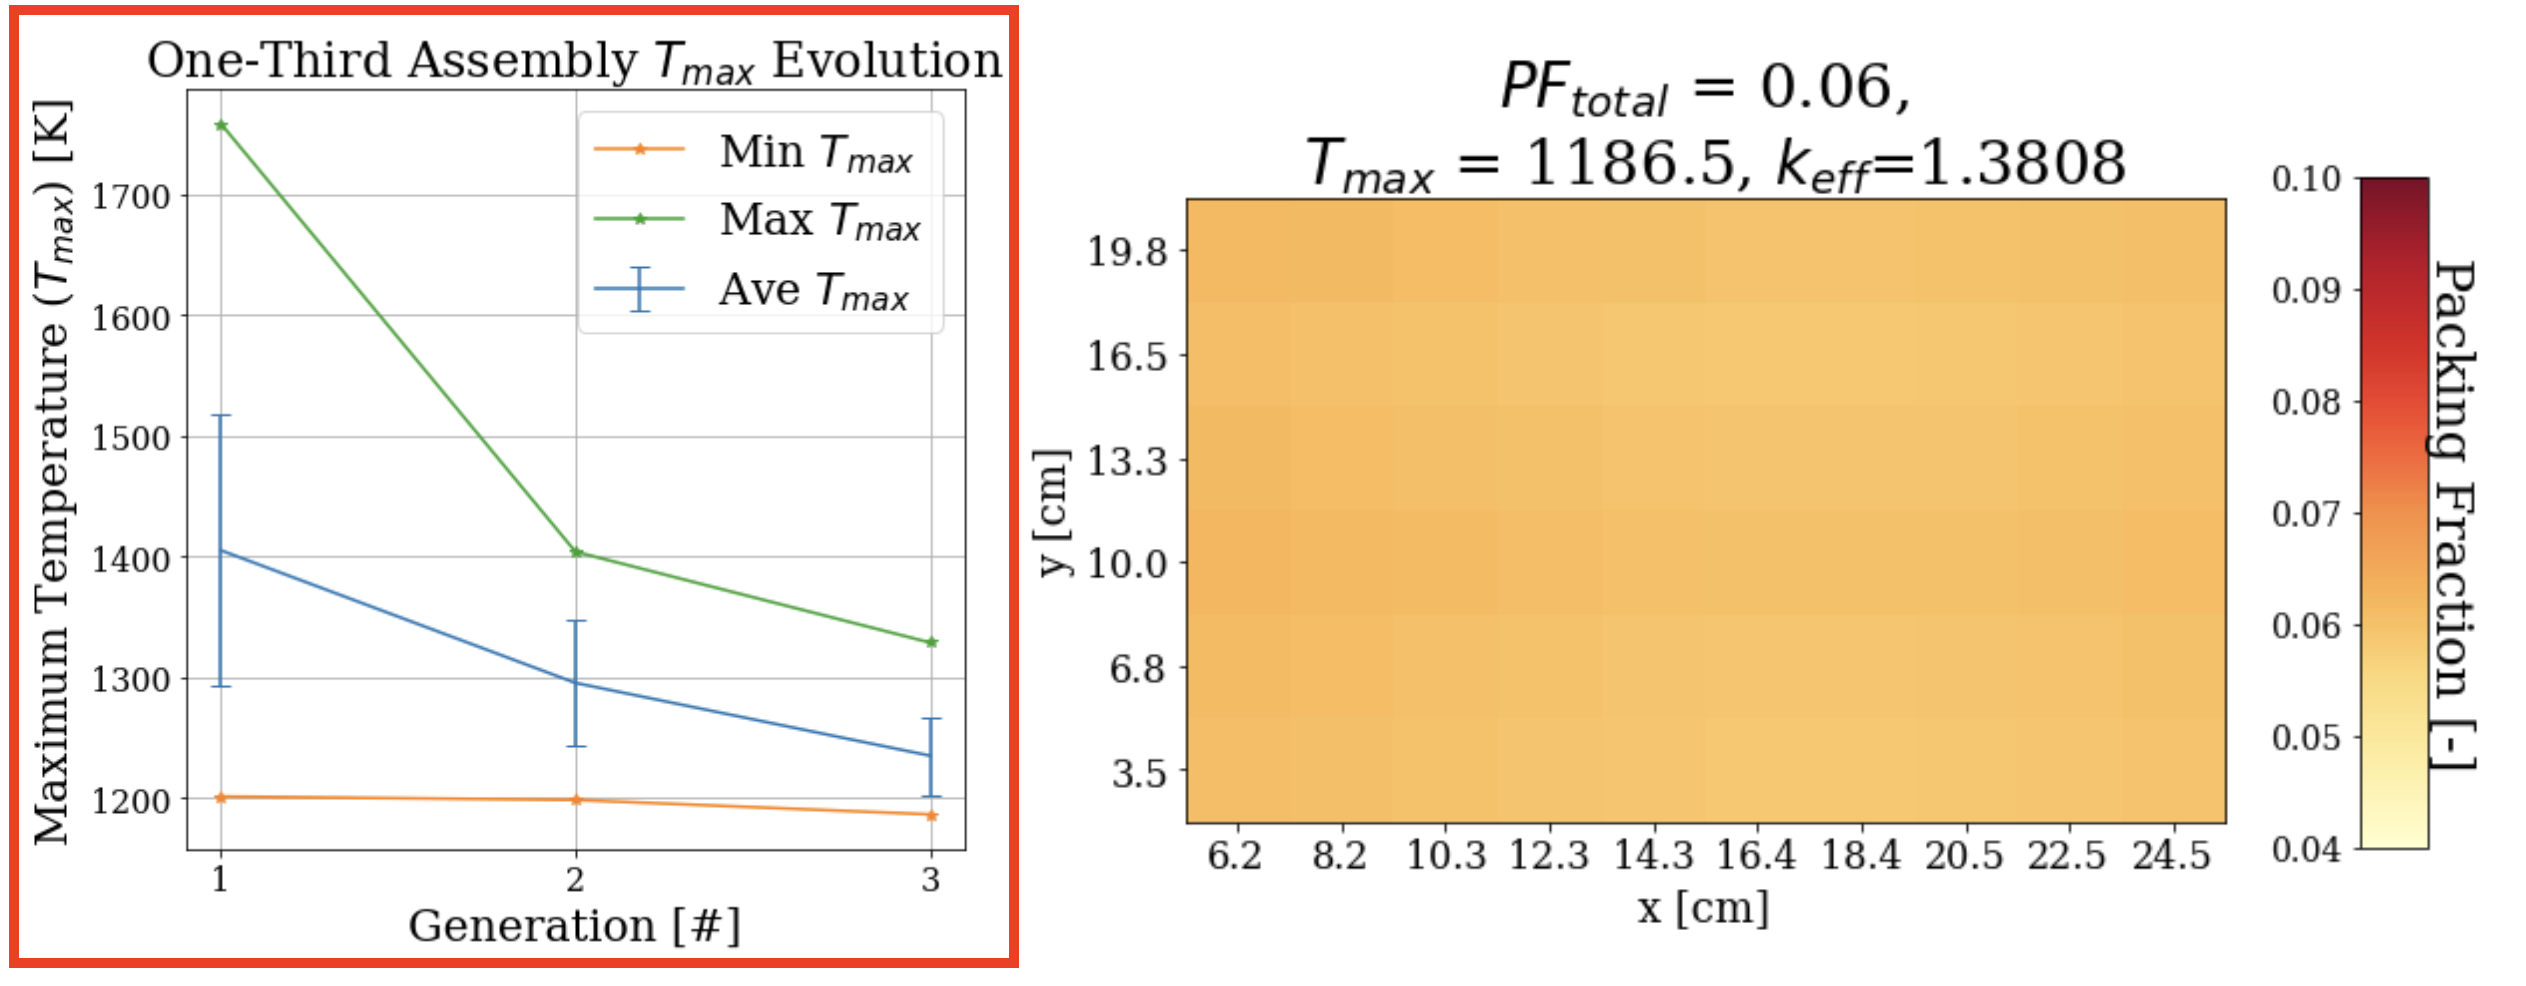
\includegraphics[width=\linewidth]{figures/assem-obj-1-temp-annotated1.png}}
        \only<3>{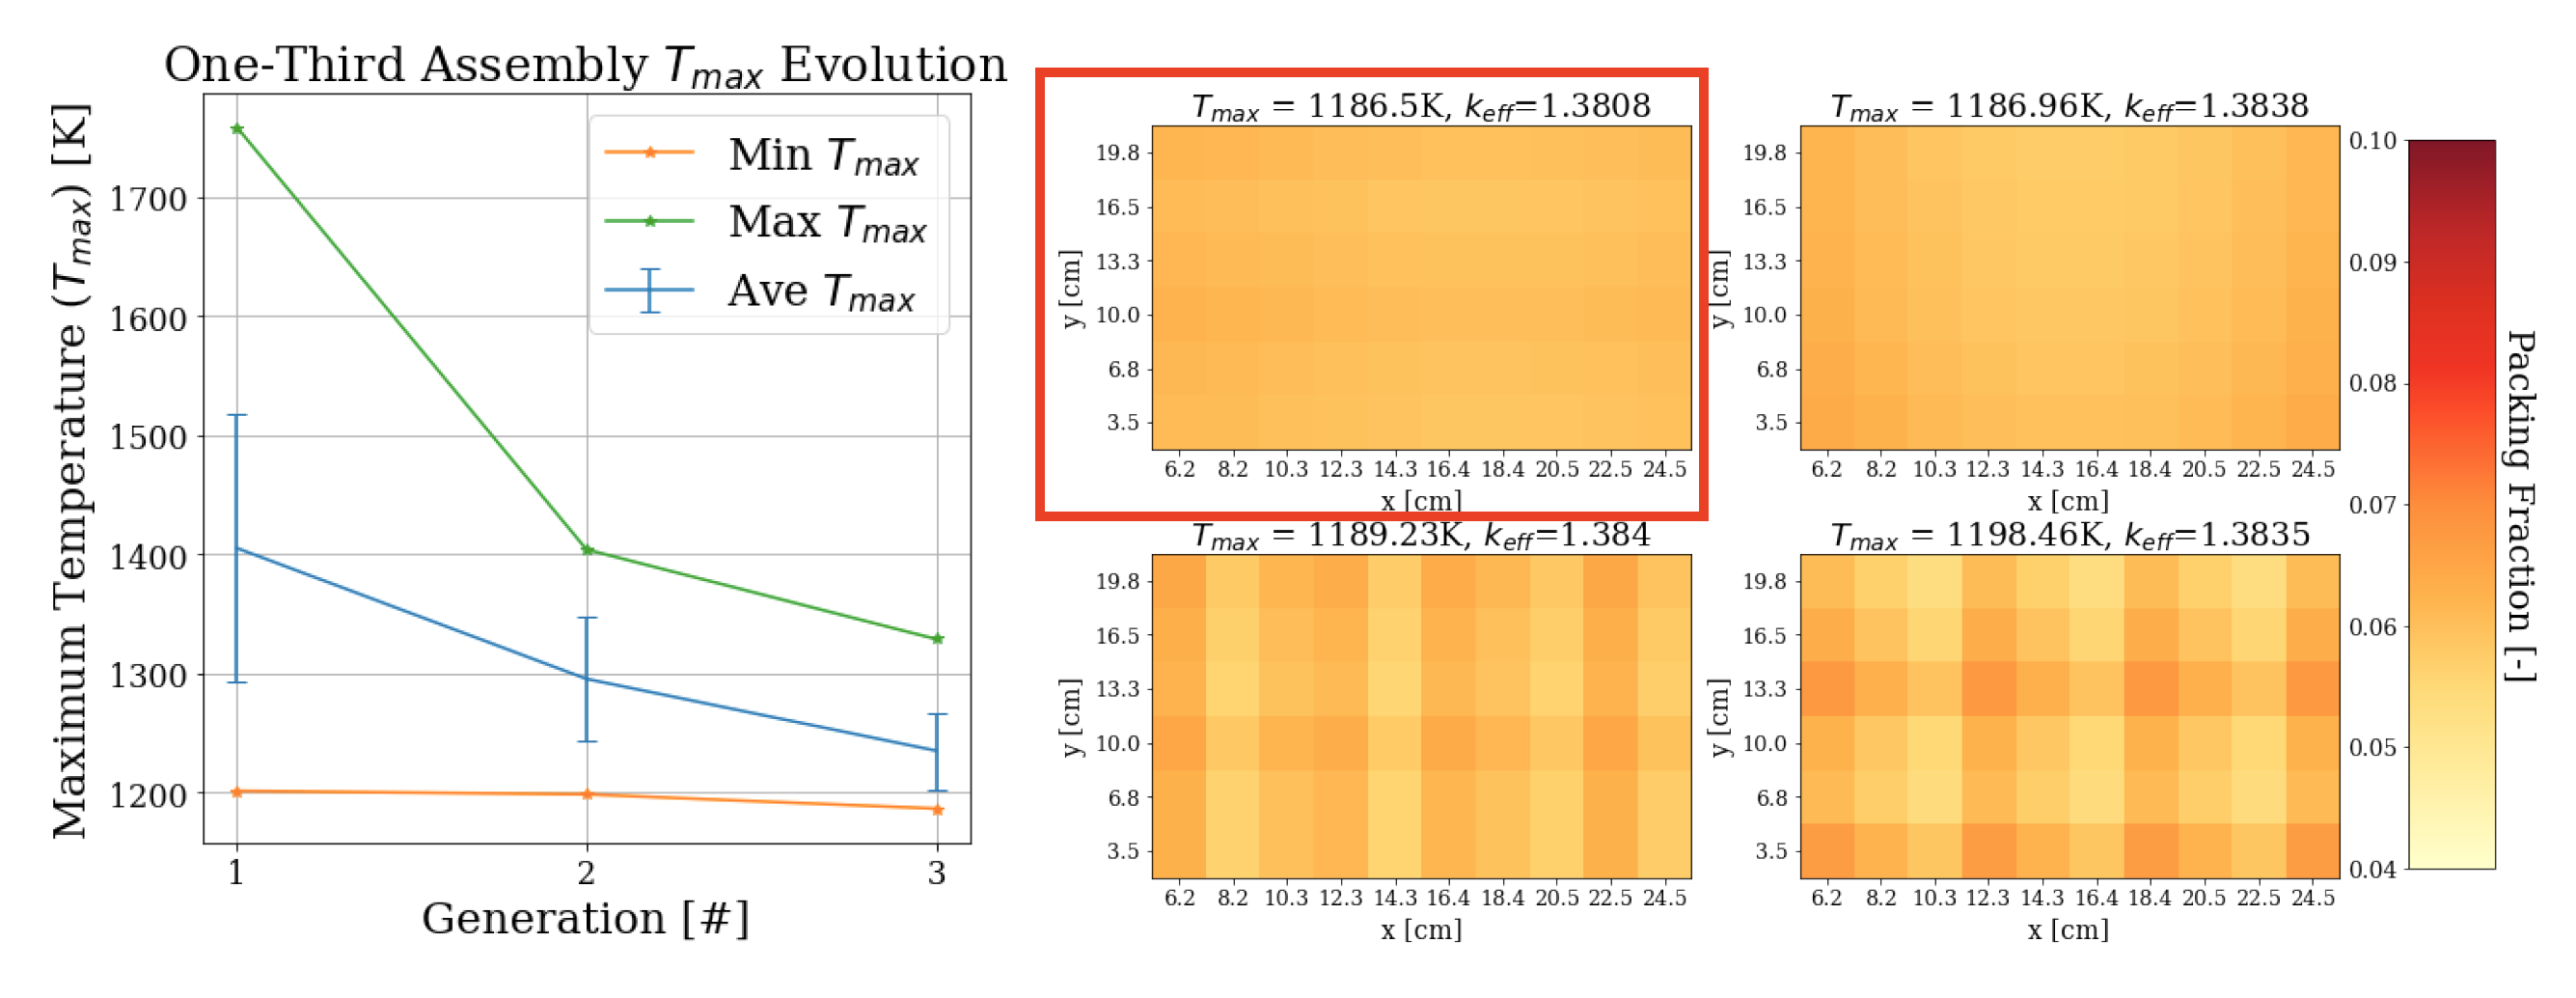
\includegraphics[width=\linewidth]{figures/assem-obj-1-temp-annotated2.png}}
        \vspace{-0.3cm}
        \caption{Simulation a-1b $T_{max}$ evolution and TRISO distribution with lowest 
        $T_{max}$.}
    \end{figure}

    \only<2>{
    \vspace{-0.2cm}
    Simulation a-1b runs for 3 generations with 128 reactor models per 
    generation, the average $T_{max}$ decreased by $\approx$ 100K per generation. 

    \textbf{The average one-third assembly $T_{max}$ converged to $\approx$ 1220K}.}

    \only<3>{\textbf{The TRISO distribution in the final generation with the 
    lowest $T_{max}$ has $T_{max}$ = 1186K and an almost constant TRISO packing fraction 
    distribution.}}

    \only<4>{
    \vspace{-0.4cm}    
    \begin{tcolorbox}[colback=illiniorange,colframe=illiniorange!50!black]
        \textbf{A flatter TRISO distribution minimizes $T_{max}$.}
    \end{tcolorbox}}
\end{frame}

\begin{frame}
    \frametitle{AHTR One-Third Assembly Simulation a-1e Results}
    \visible<1->{\textbf{I vary $r_1, r_2, r_3, r_4, r_5$ (coolant channel shape)
    to minimize $T_{max}$.}}

    \begin{figure}
        \centering
        \begin{subfigure}{0.3\textwidth}
            \only<1,3>{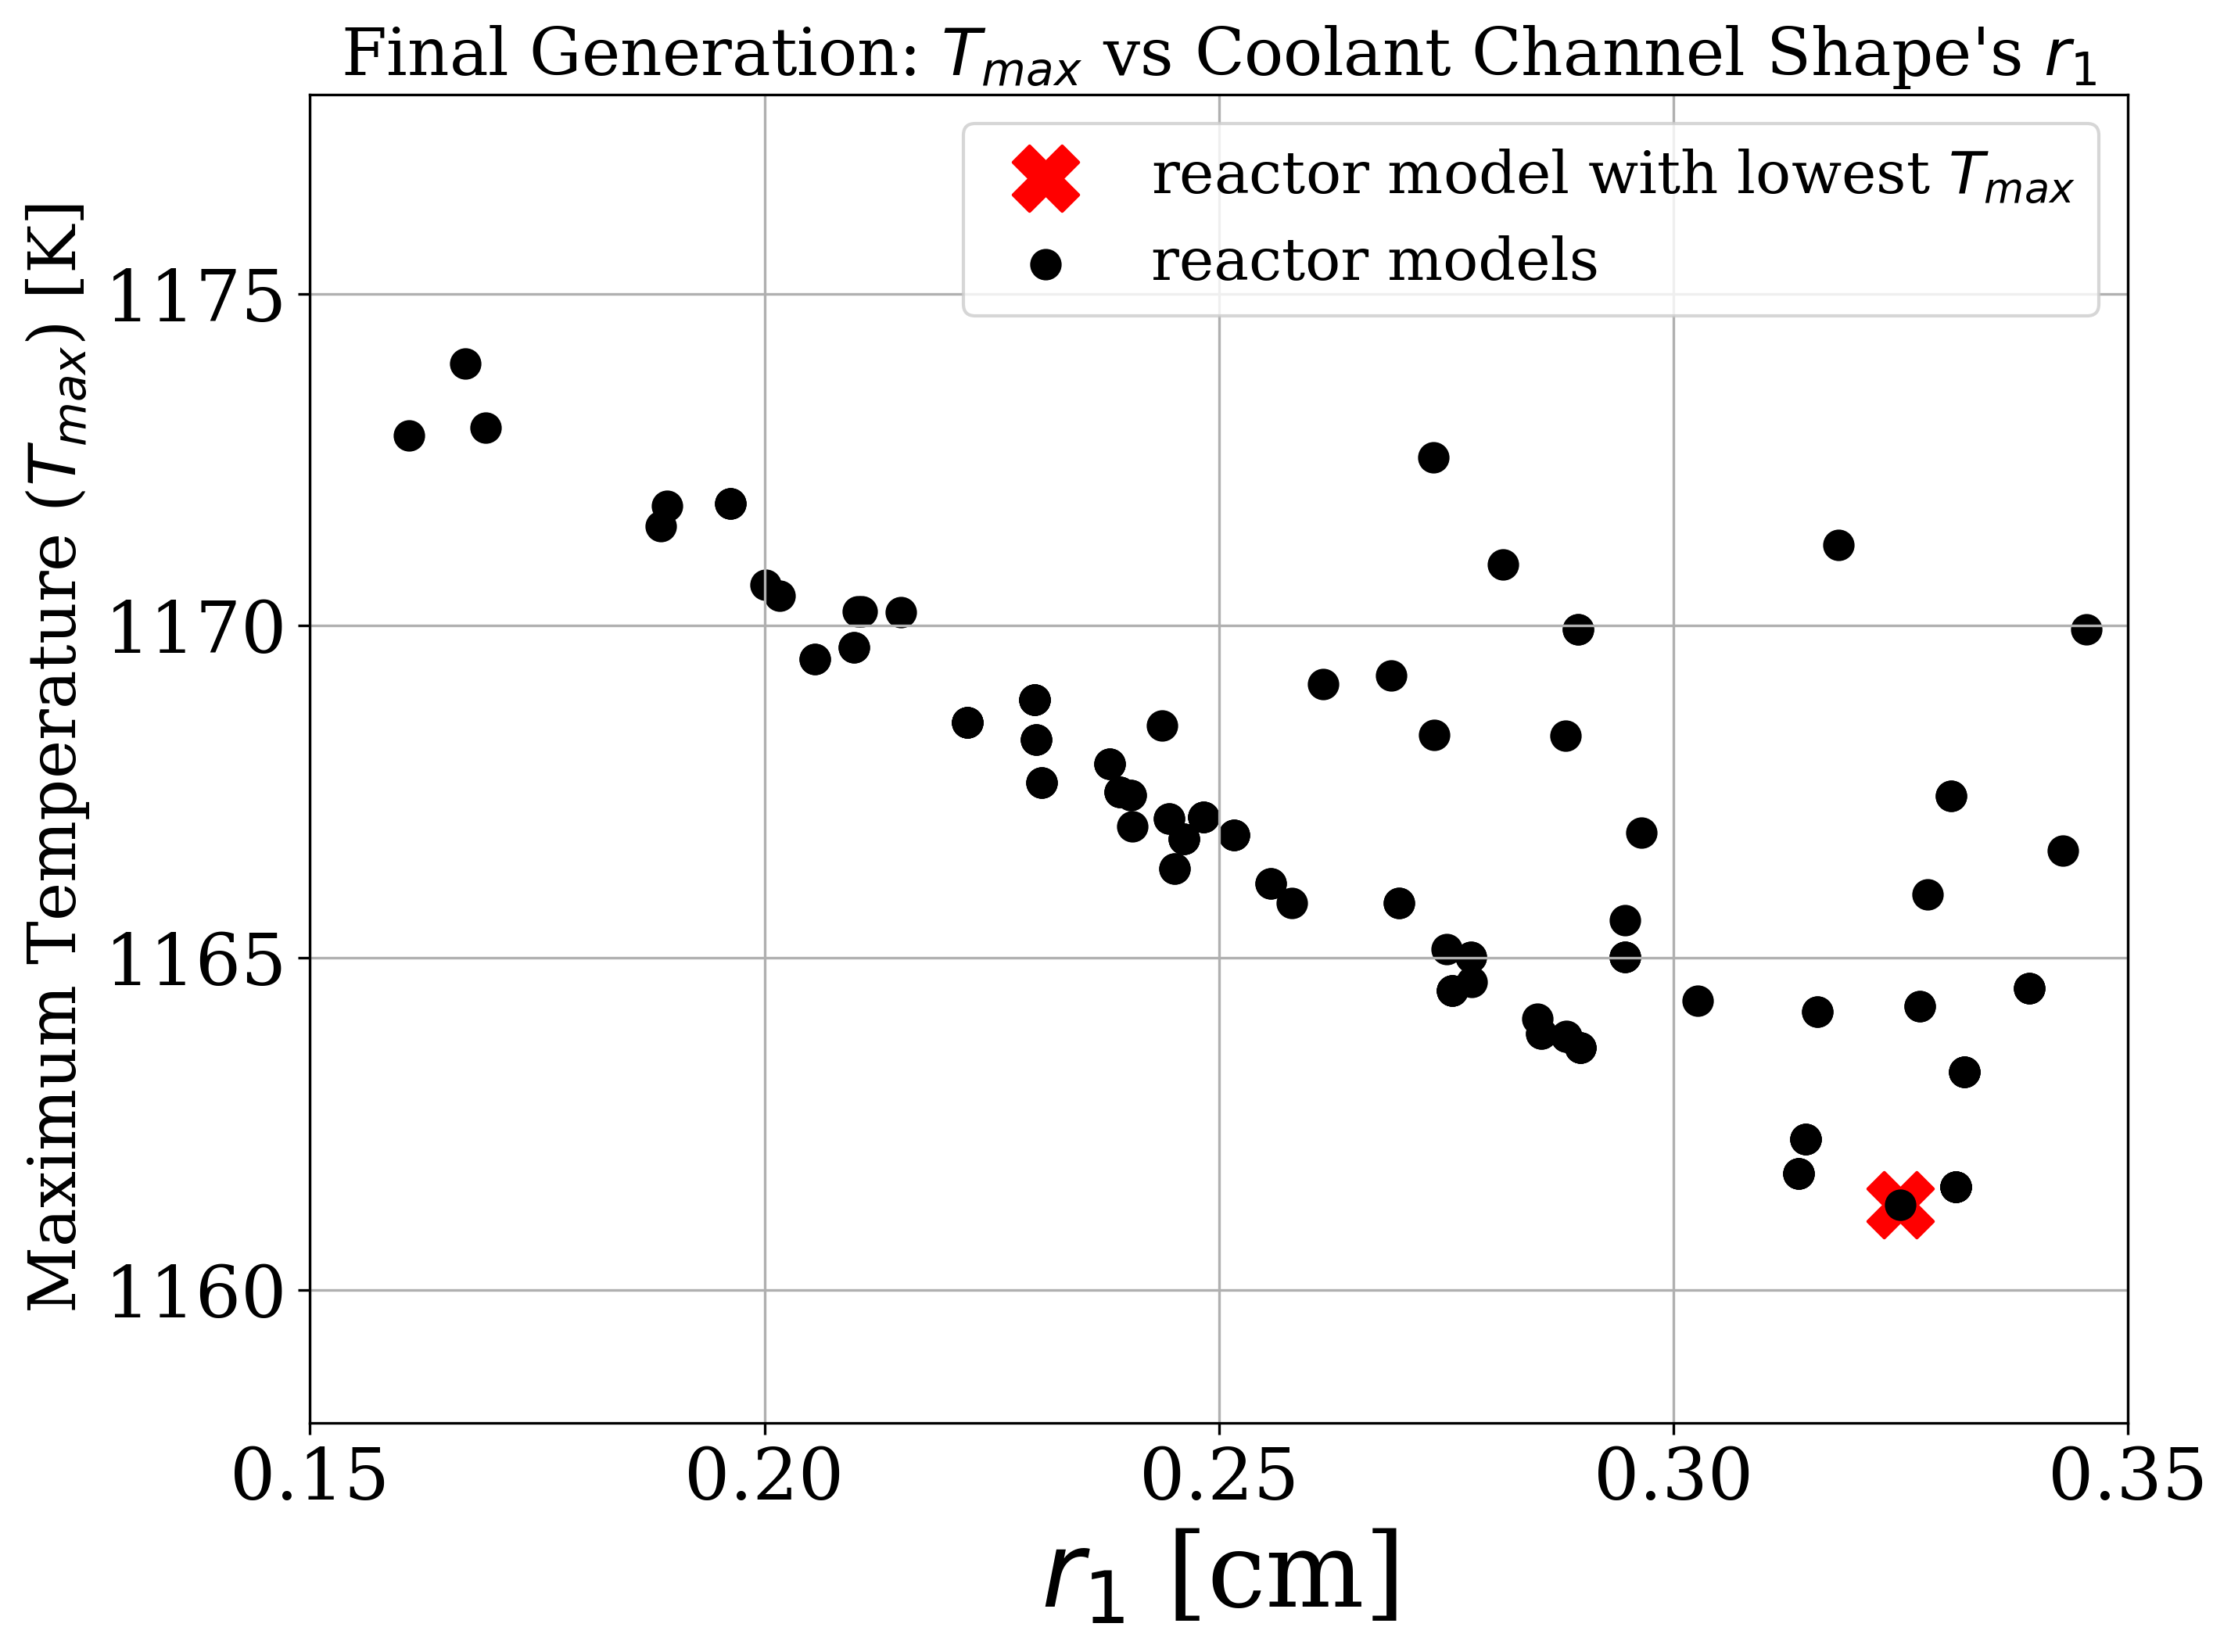
\includegraphics[width=\linewidth]{figures/a-1e-r1-pres.png}}
            \only<2>{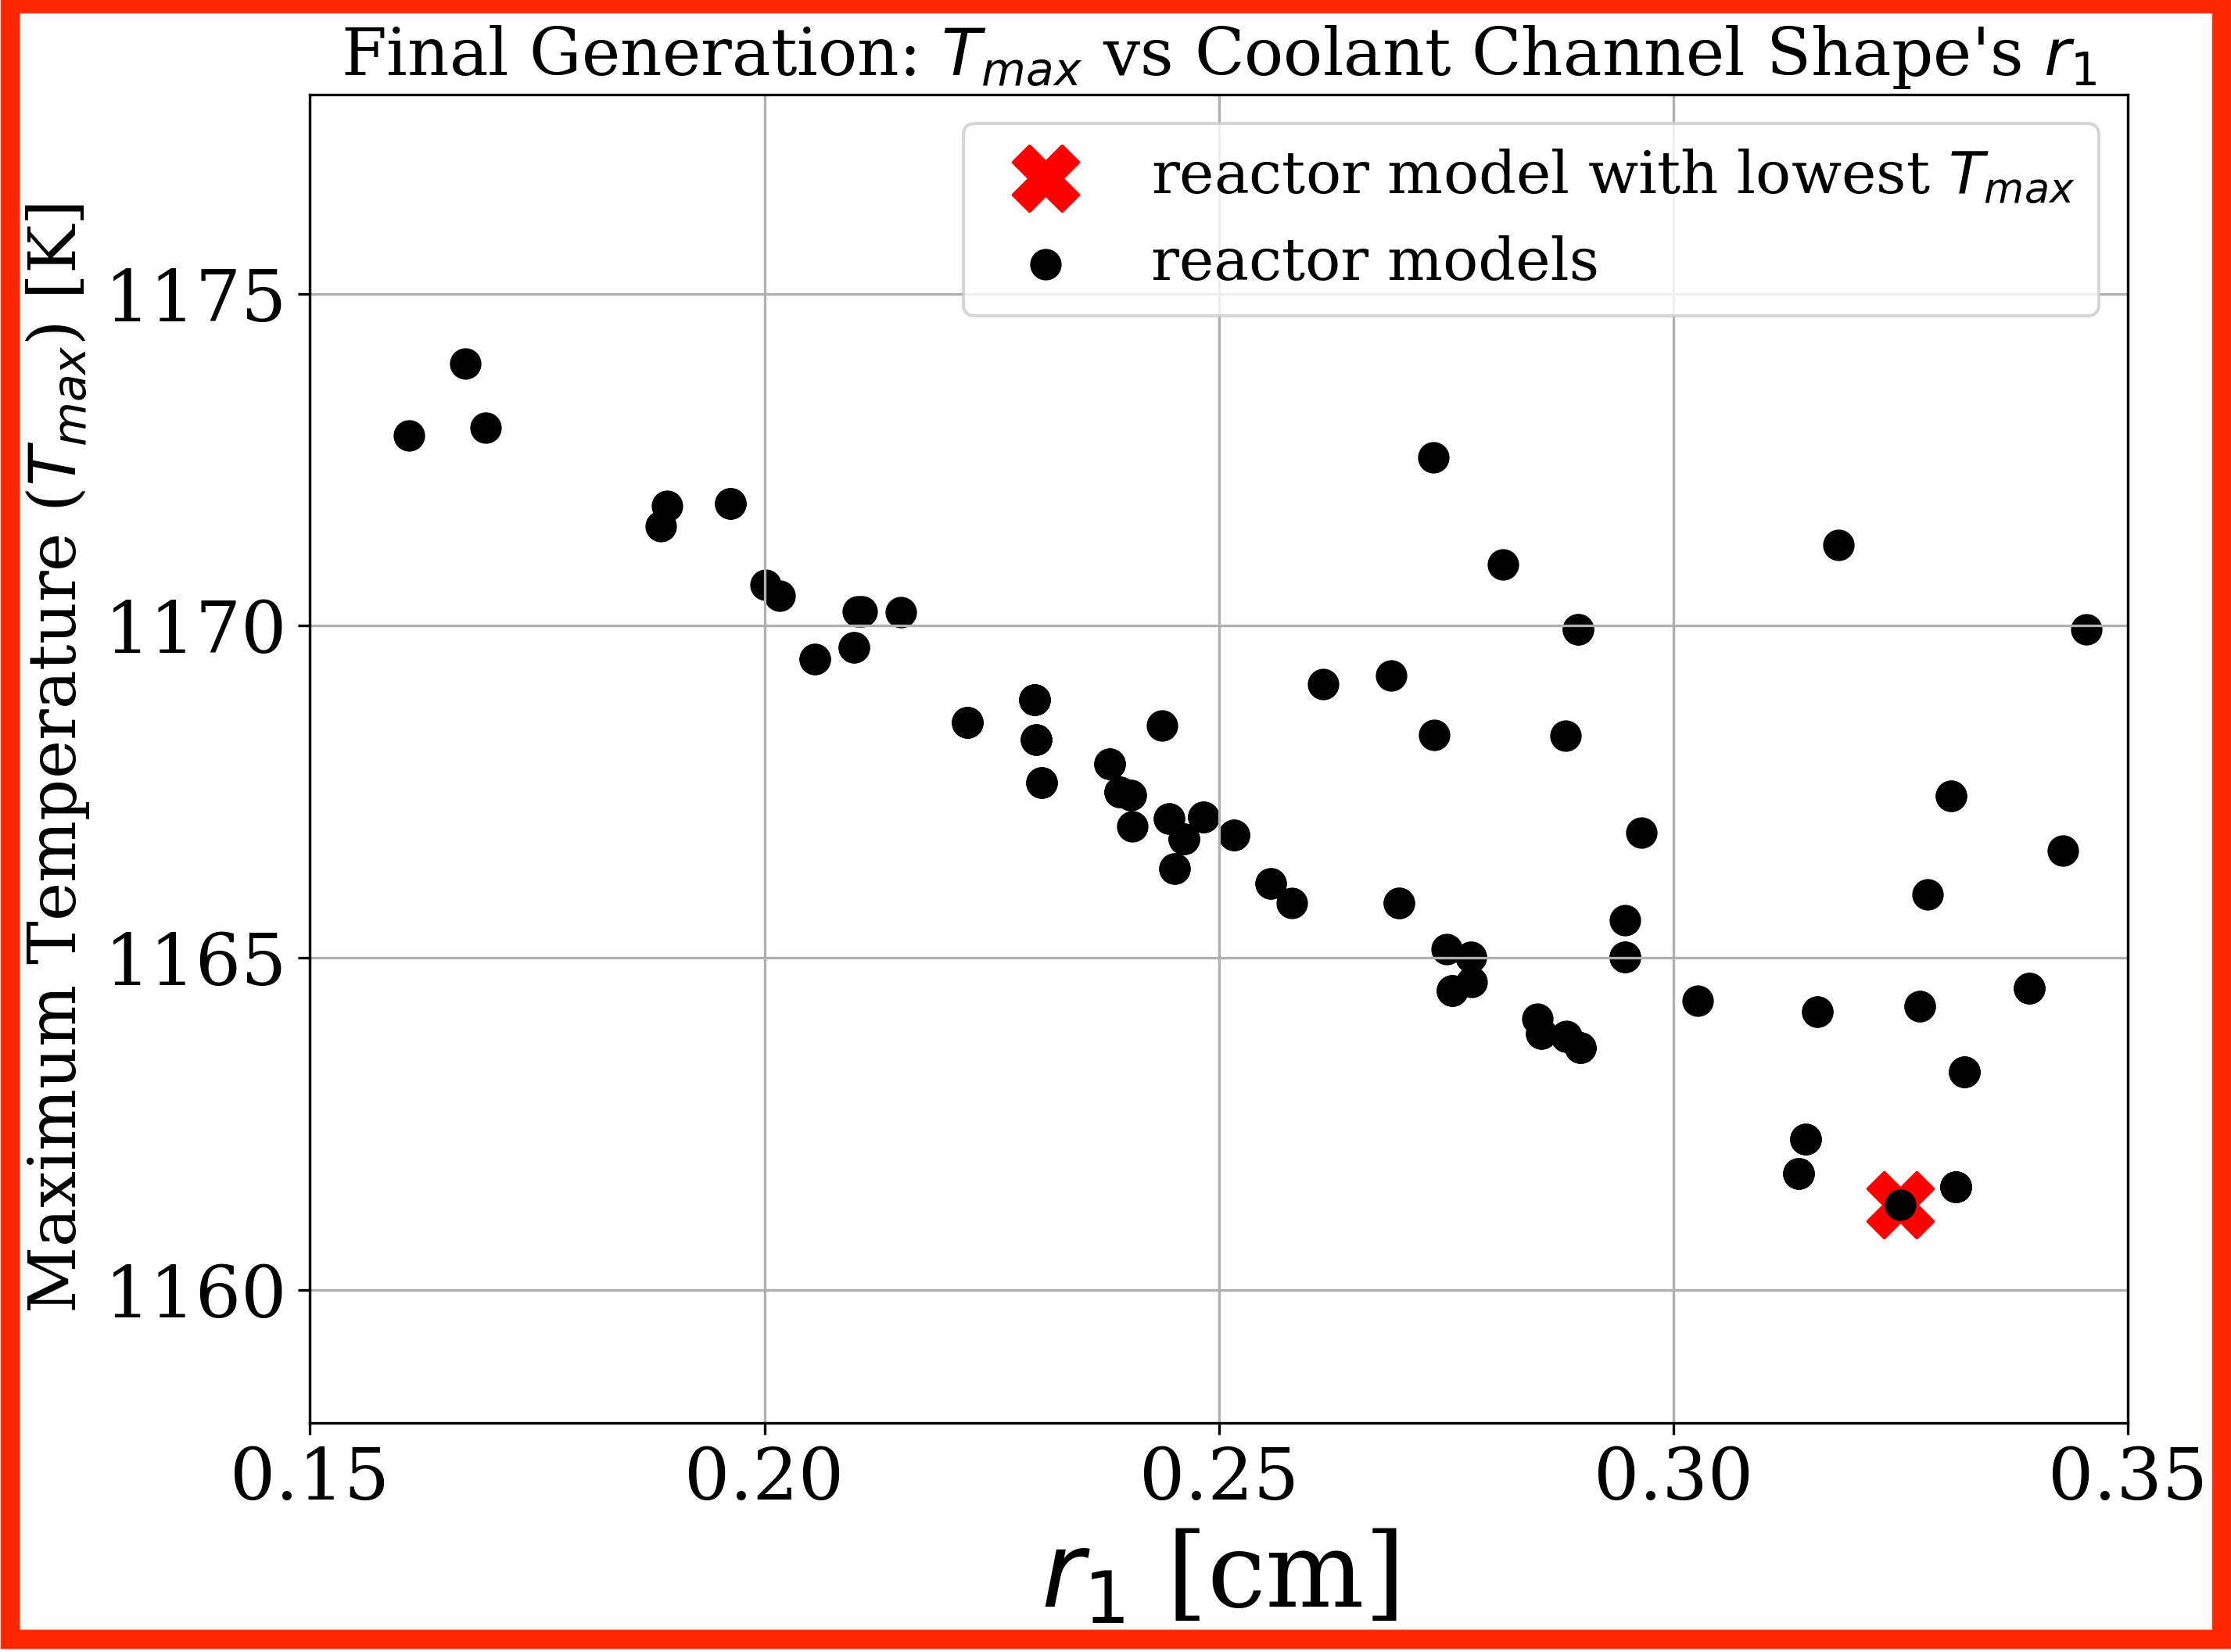
\includegraphics[width=\linewidth]{figures/a-1e-r1-pres-annotated.png}}
            \vspace{-0.5cm}
            \caption{Plot of $T_{max}$ against $r_1$.}
        \end{subfigure}
        \begin{subfigure}{0.3\textwidth}
            \only<1,2>{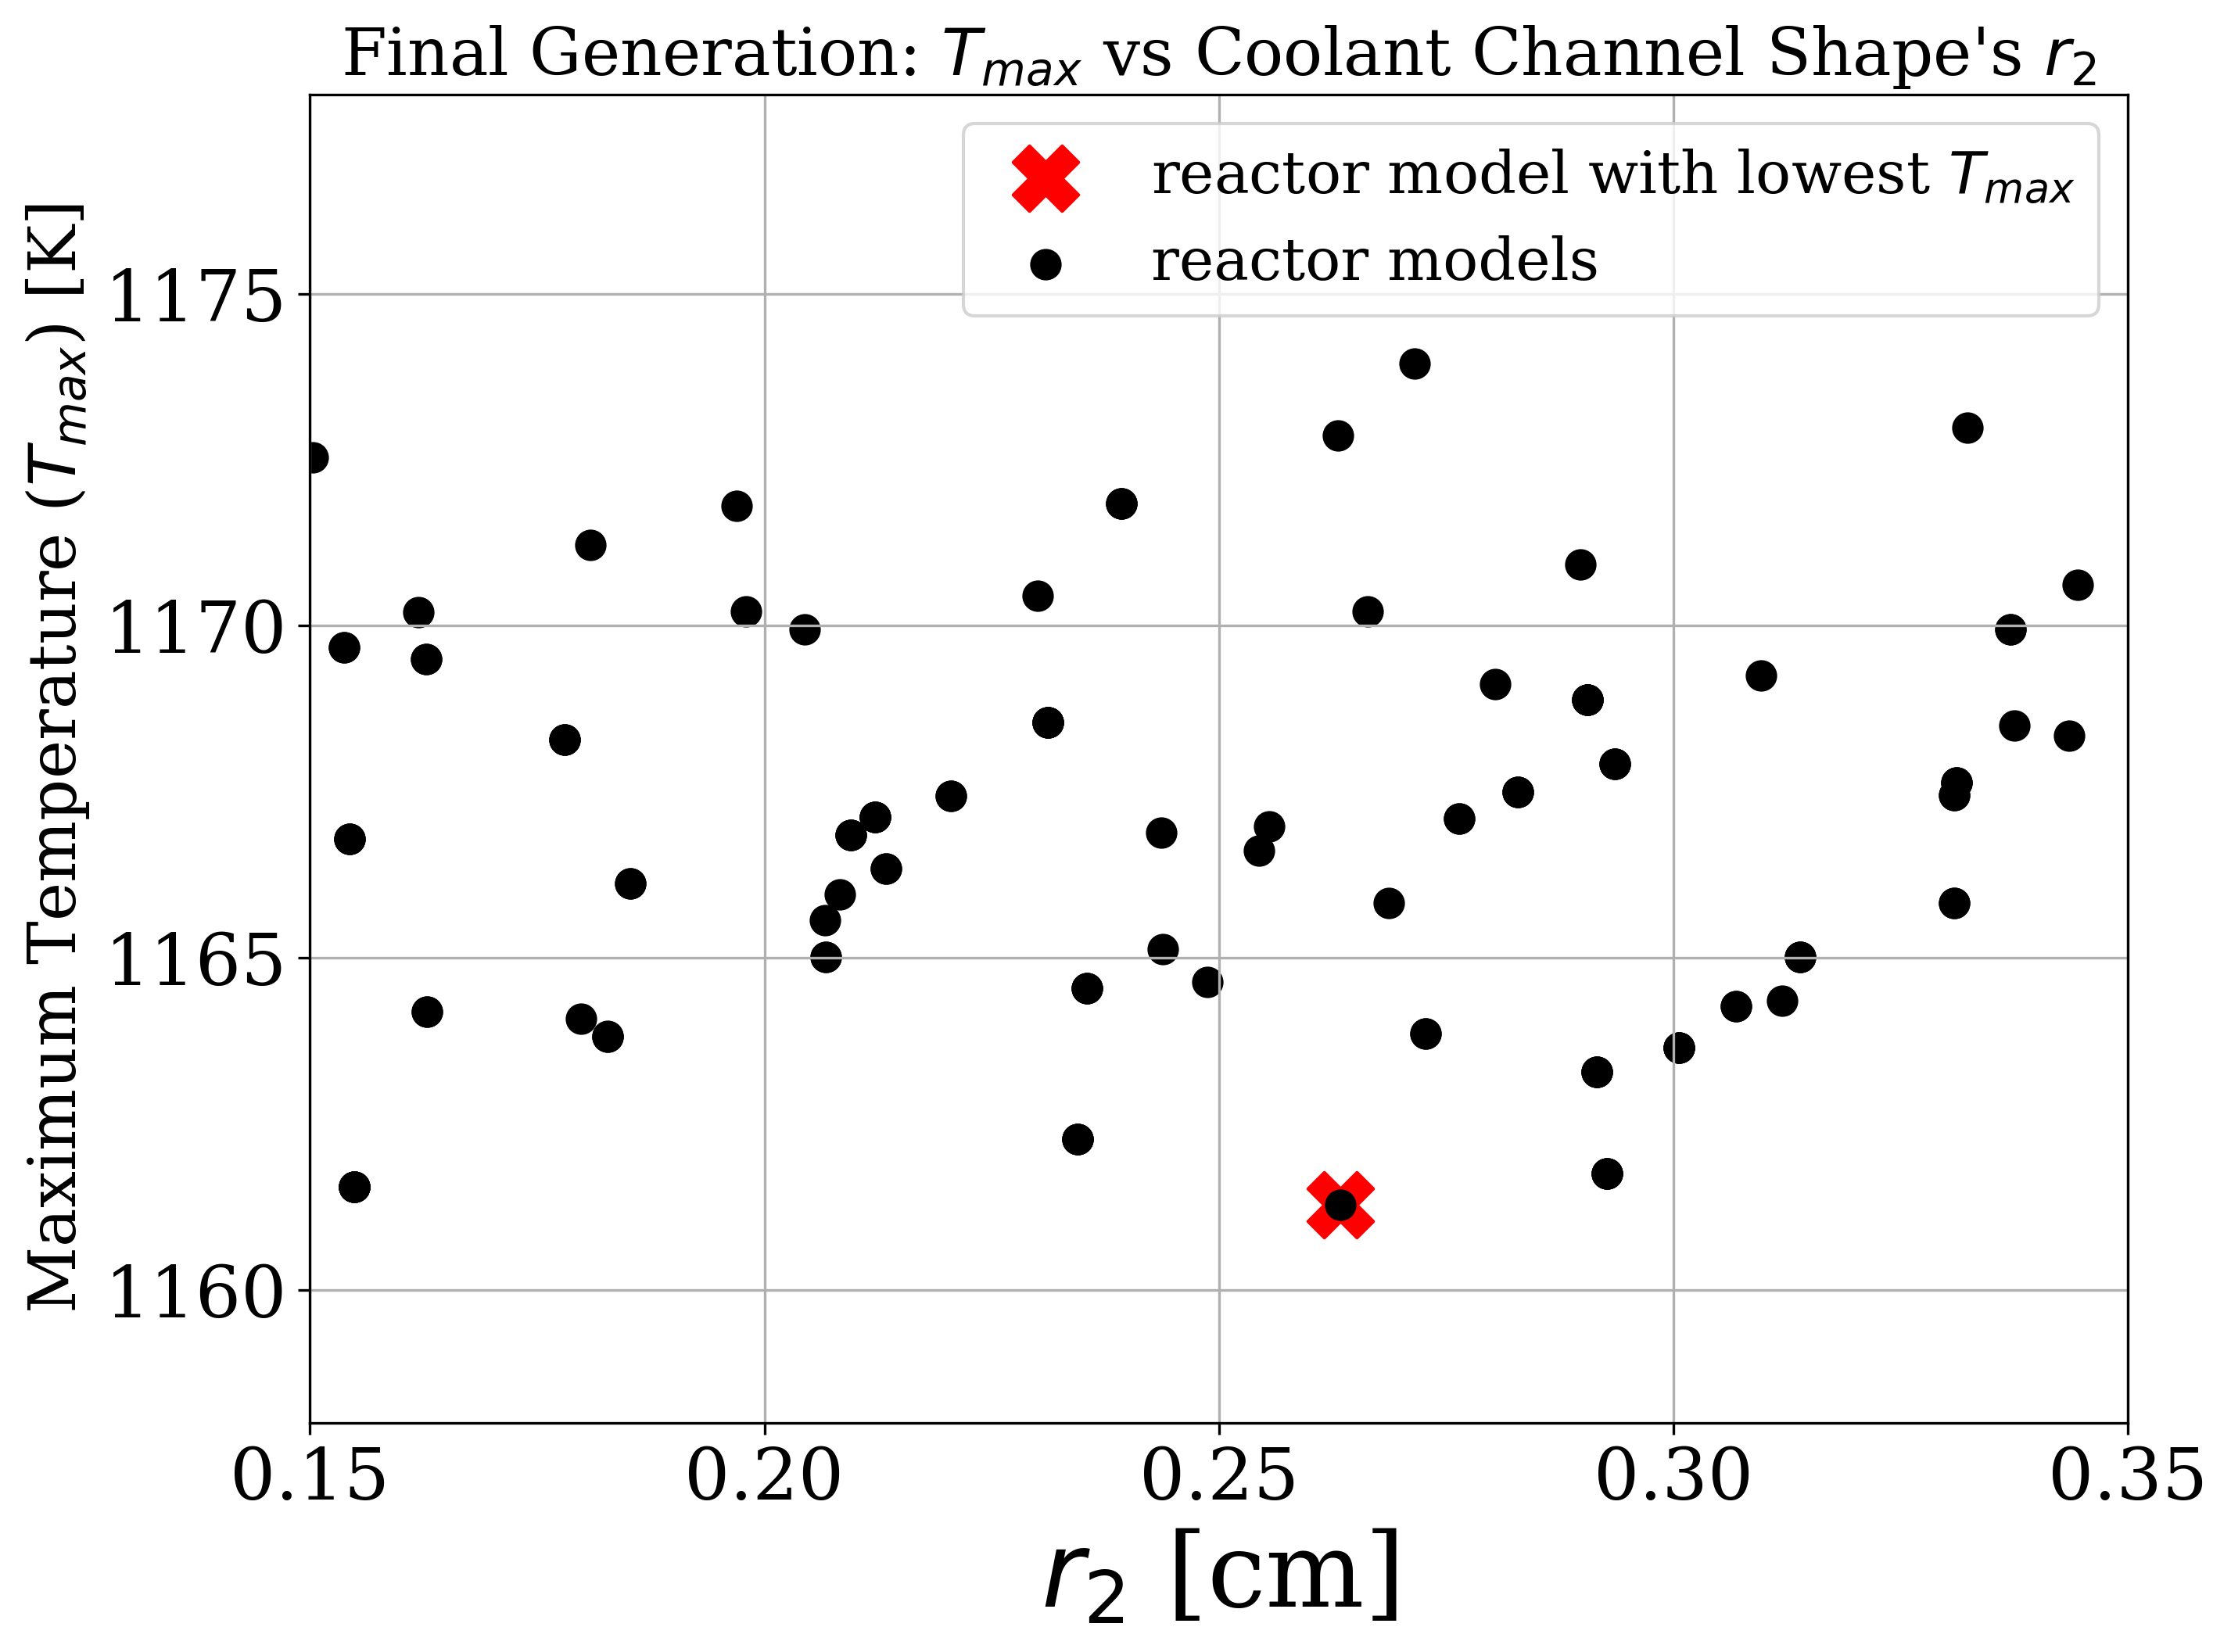
\includegraphics[width=\linewidth]{figures/a-1e-r2-pres.png}}
            \only<3>{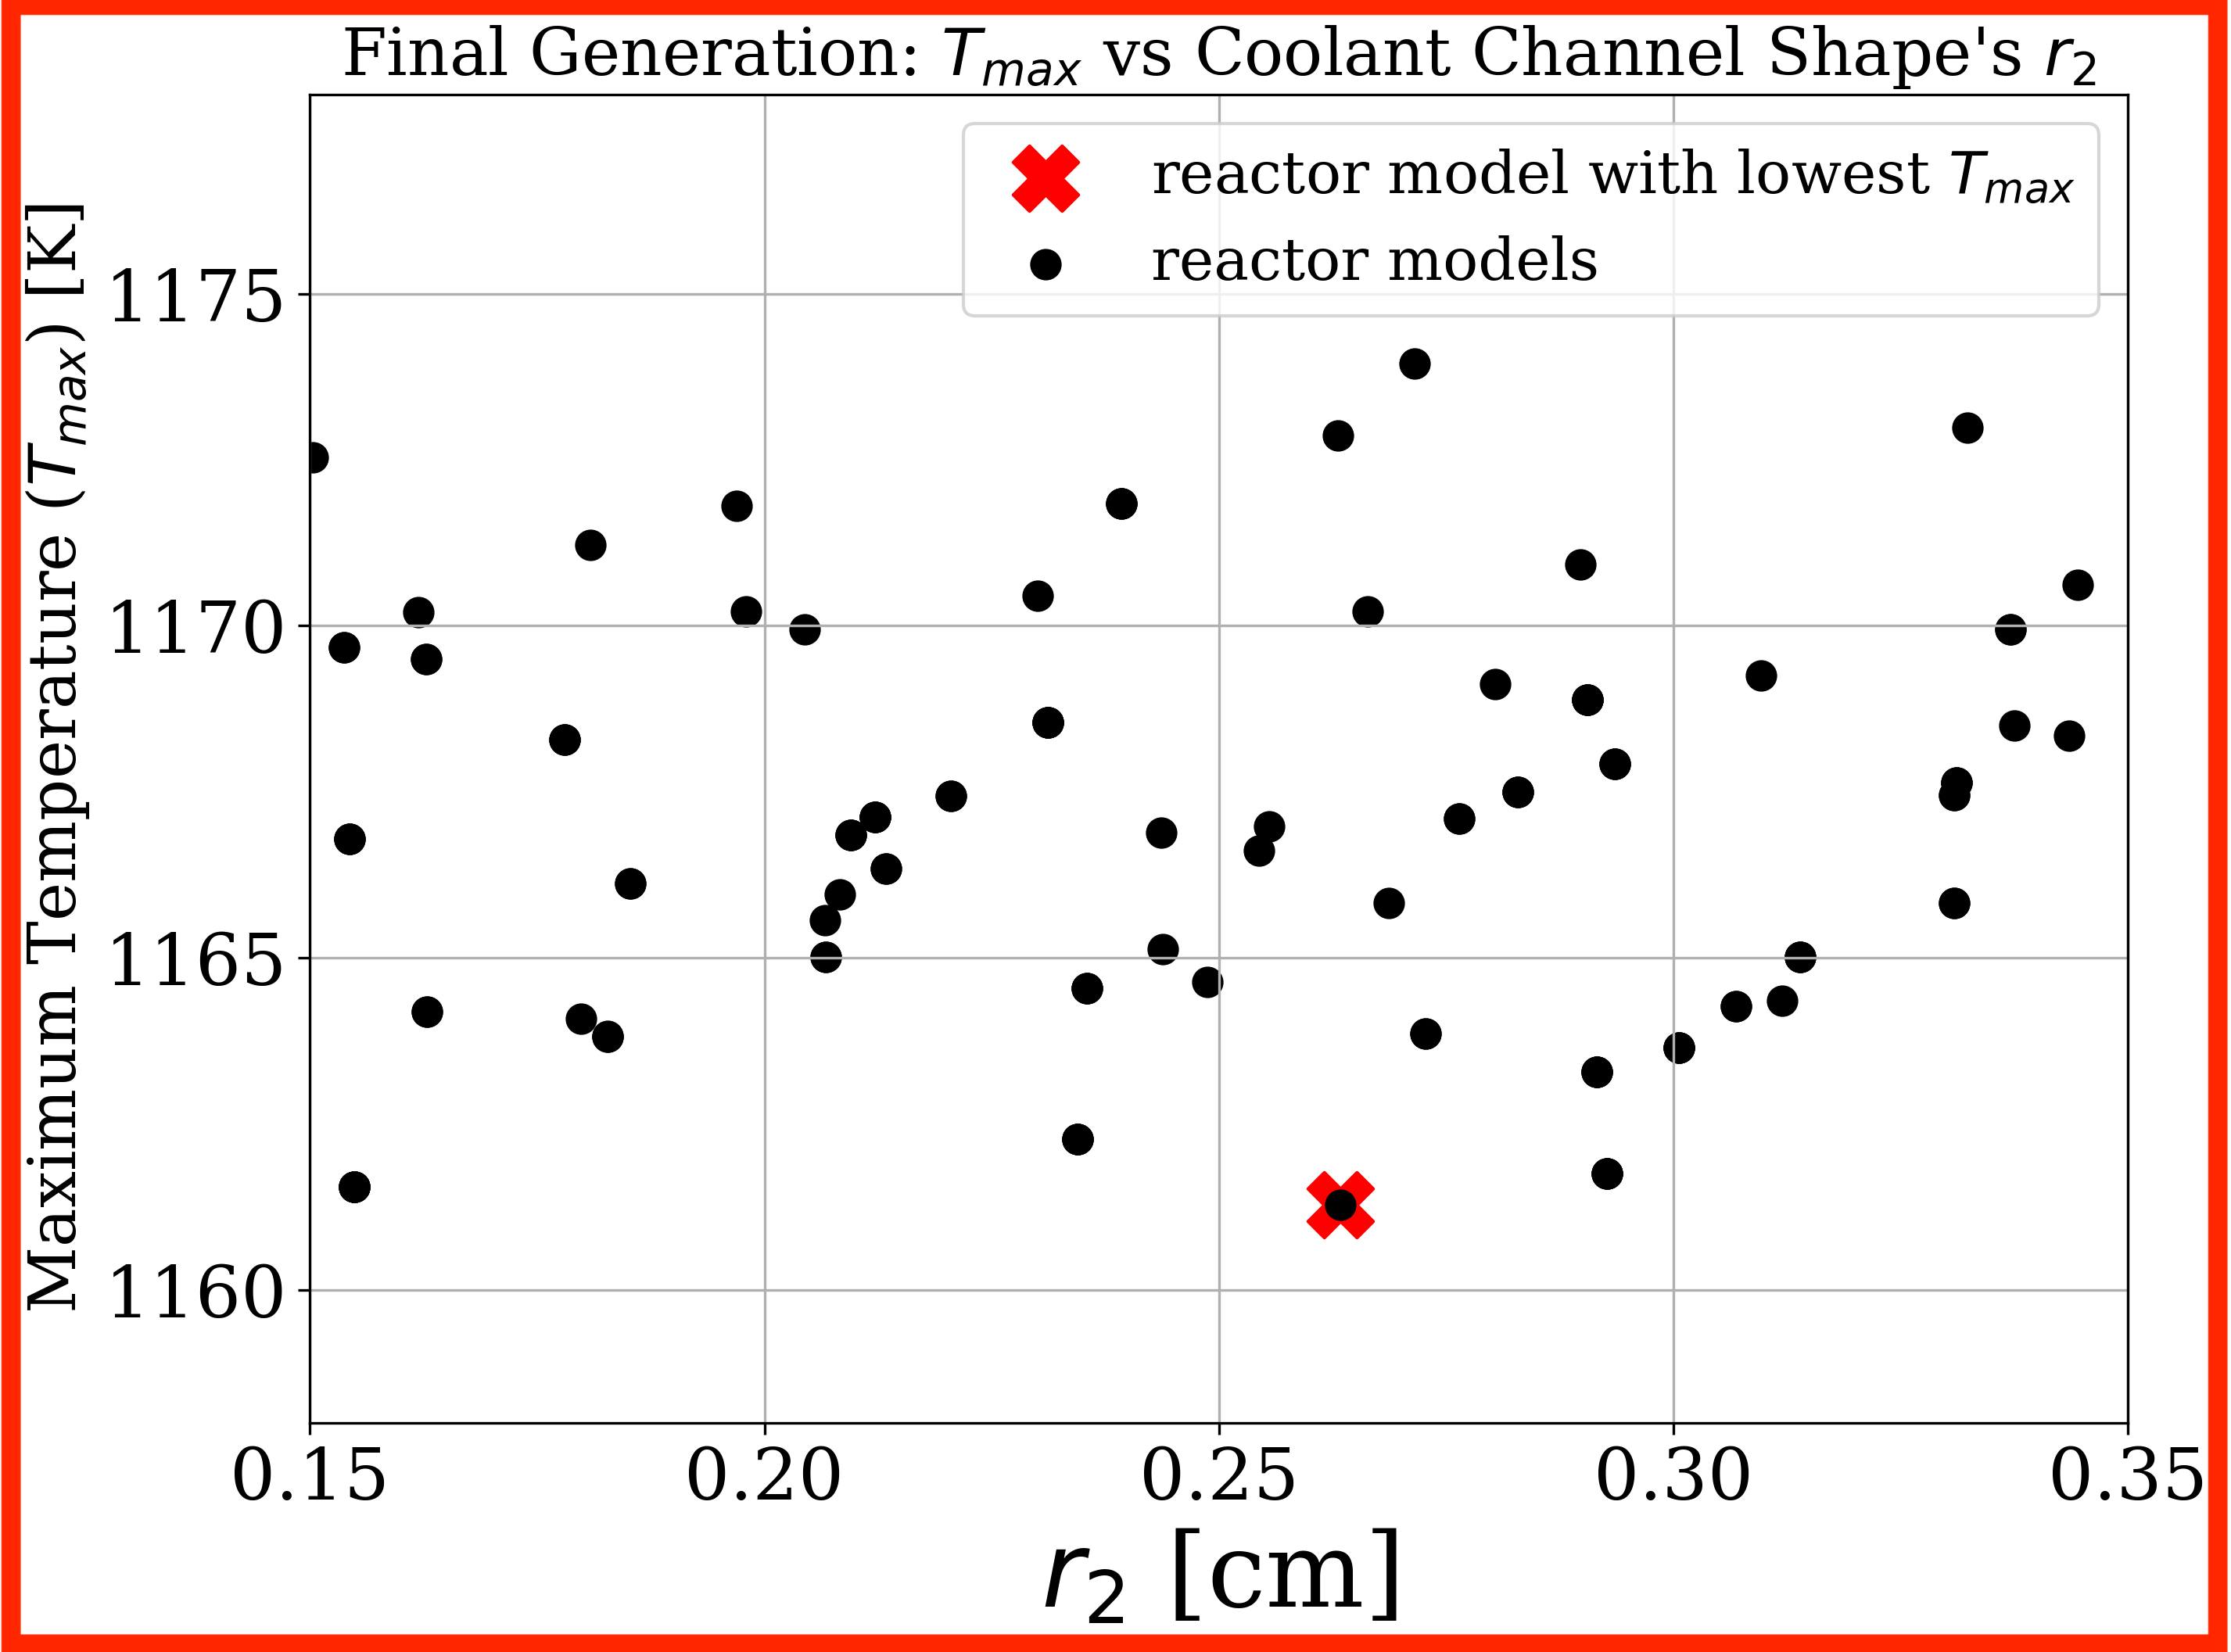
\includegraphics[width=\linewidth]{figures/a-1e-r2-pres-annotated.png}}
            \vspace{-0.5cm}
            \caption{Plot of $T_{max}$ against $r_2$.}
        \end{subfigure}
        \begin{subfigure}{0.3\textwidth}
            \only<1,2>{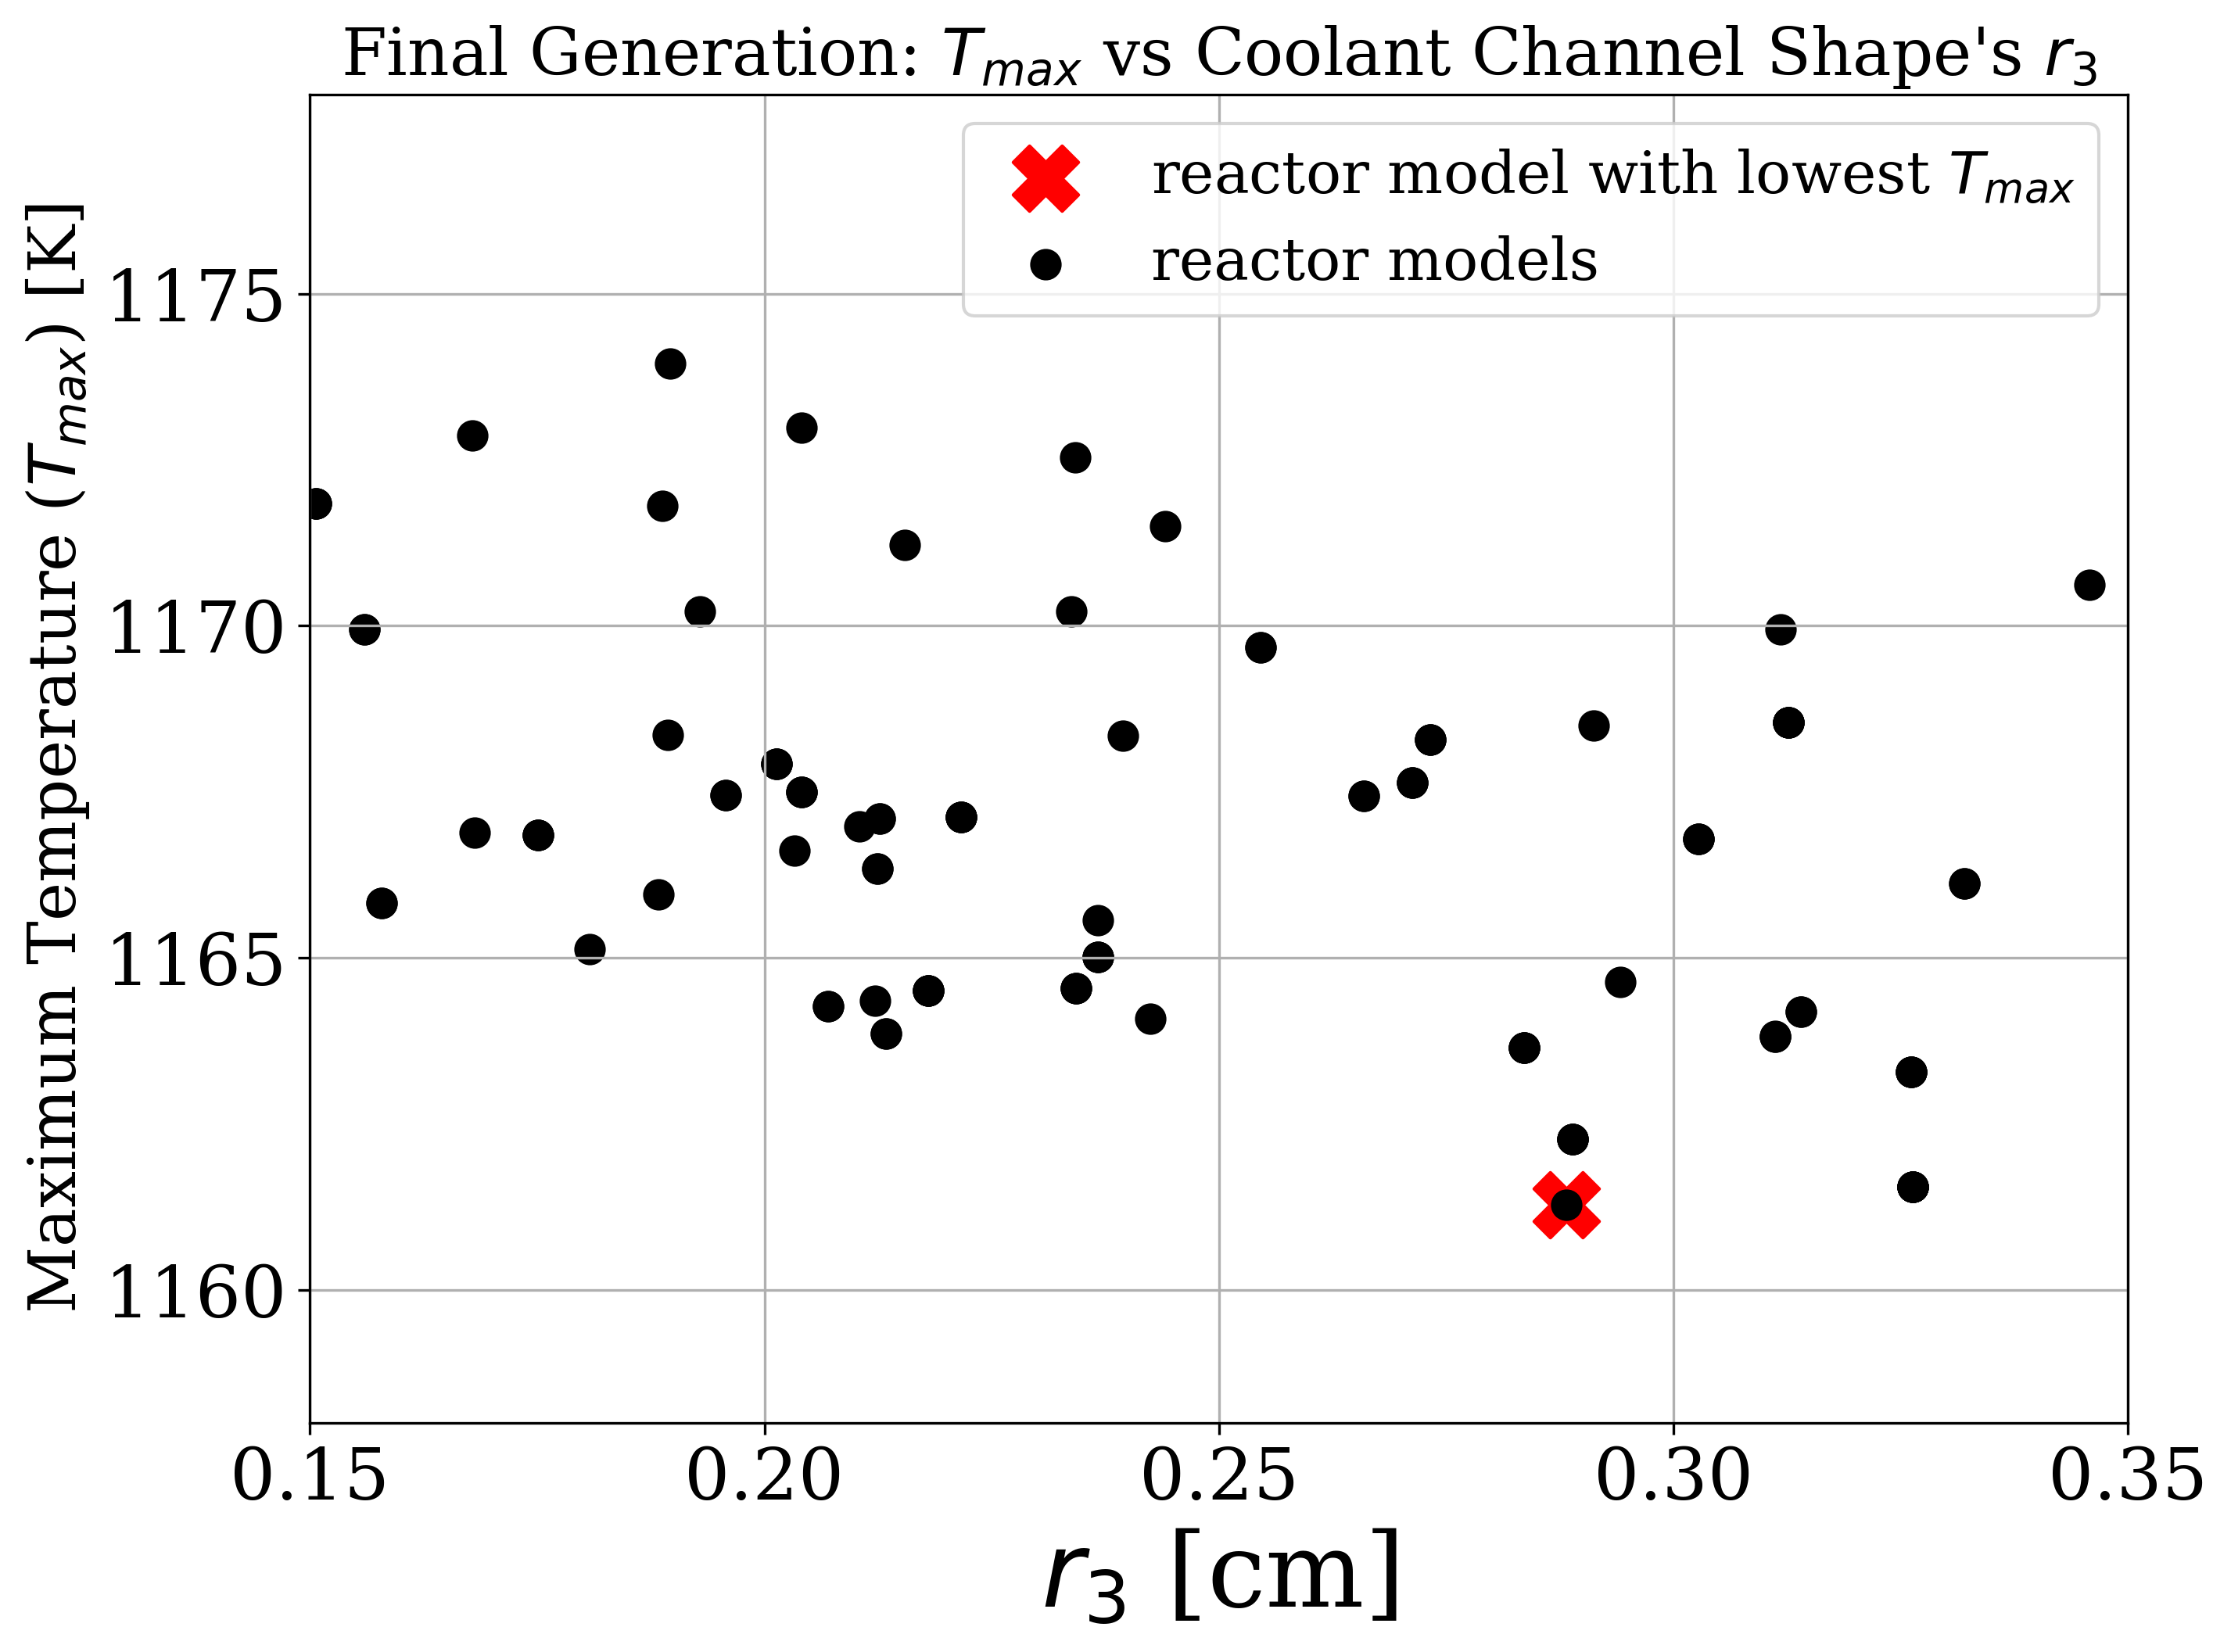
\includegraphics[width=\linewidth]{figures/a-1e-r3-pres.png}}
            \only<3>{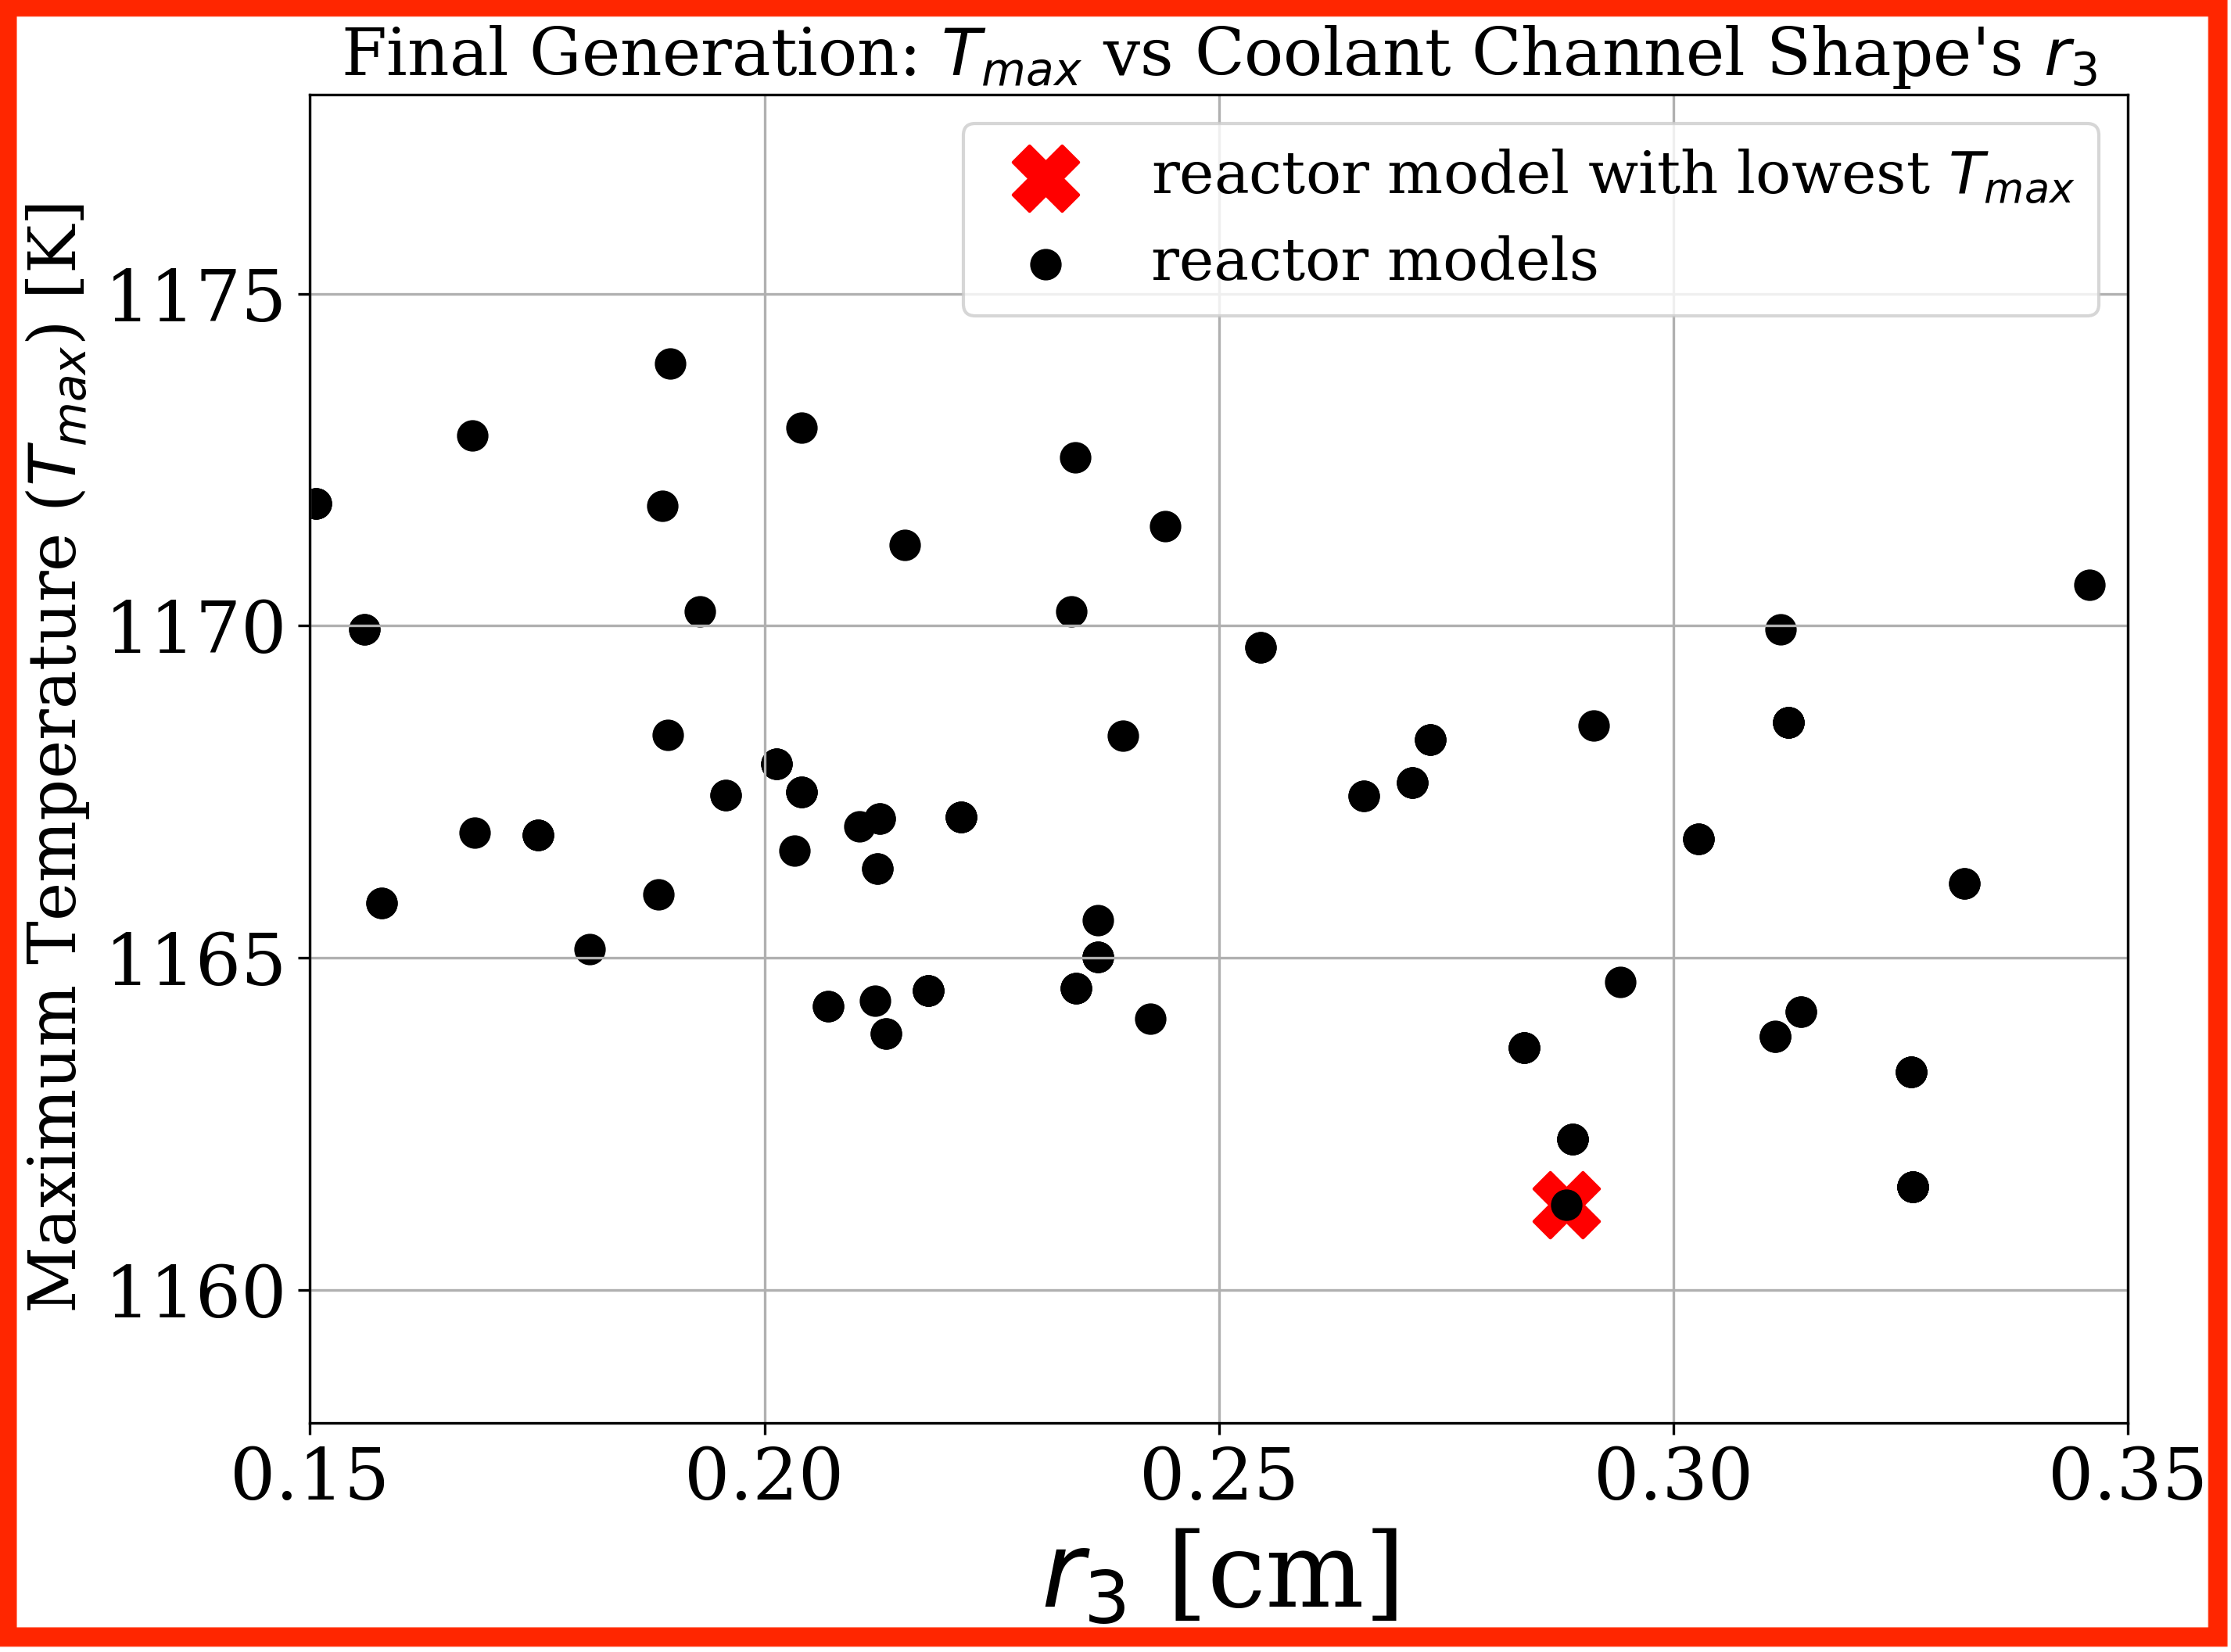
\includegraphics[width=\linewidth]{figures/a-1e-r3-pres-annotated.png}}
            \vspace{-0.5cm}
            \caption{Plot of $T_{max}$ against $r_3$.}
        \end{subfigure}
        \begin{subfigure}{0.3\textwidth}
            \only<1,2>{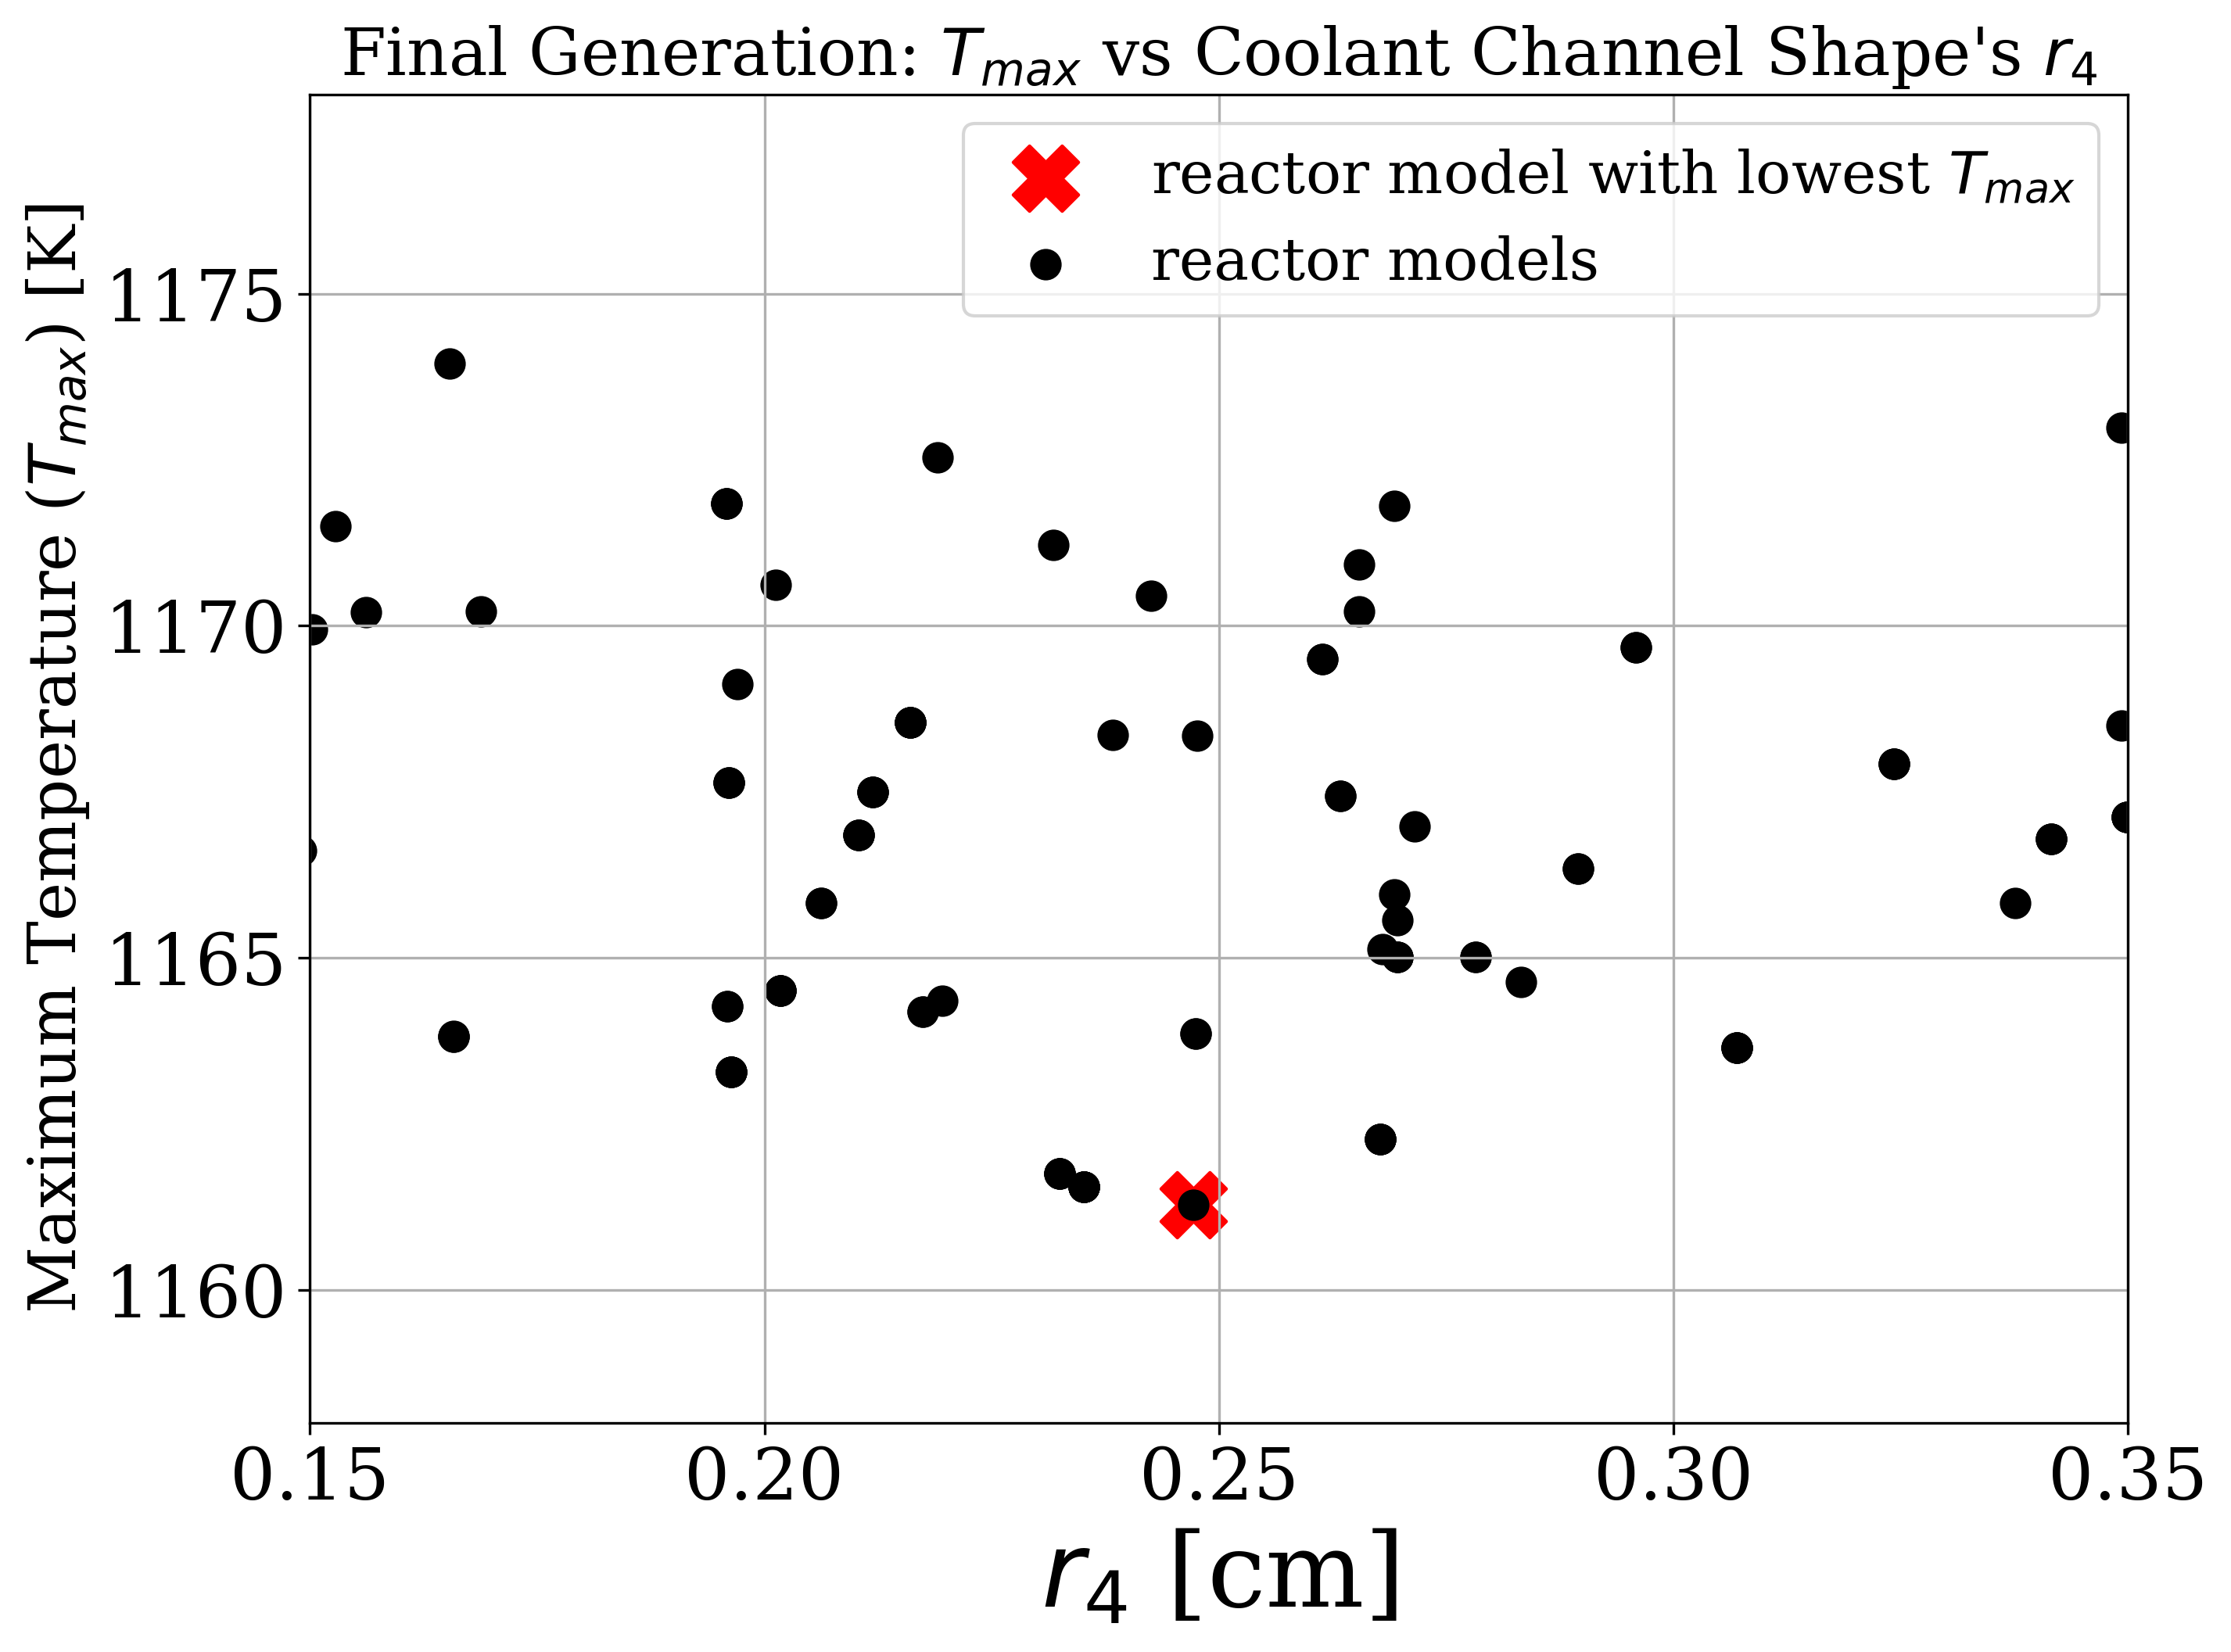
\includegraphics[width=\linewidth]{figures/a-1e-r4-pres.png}}
            \only<3>{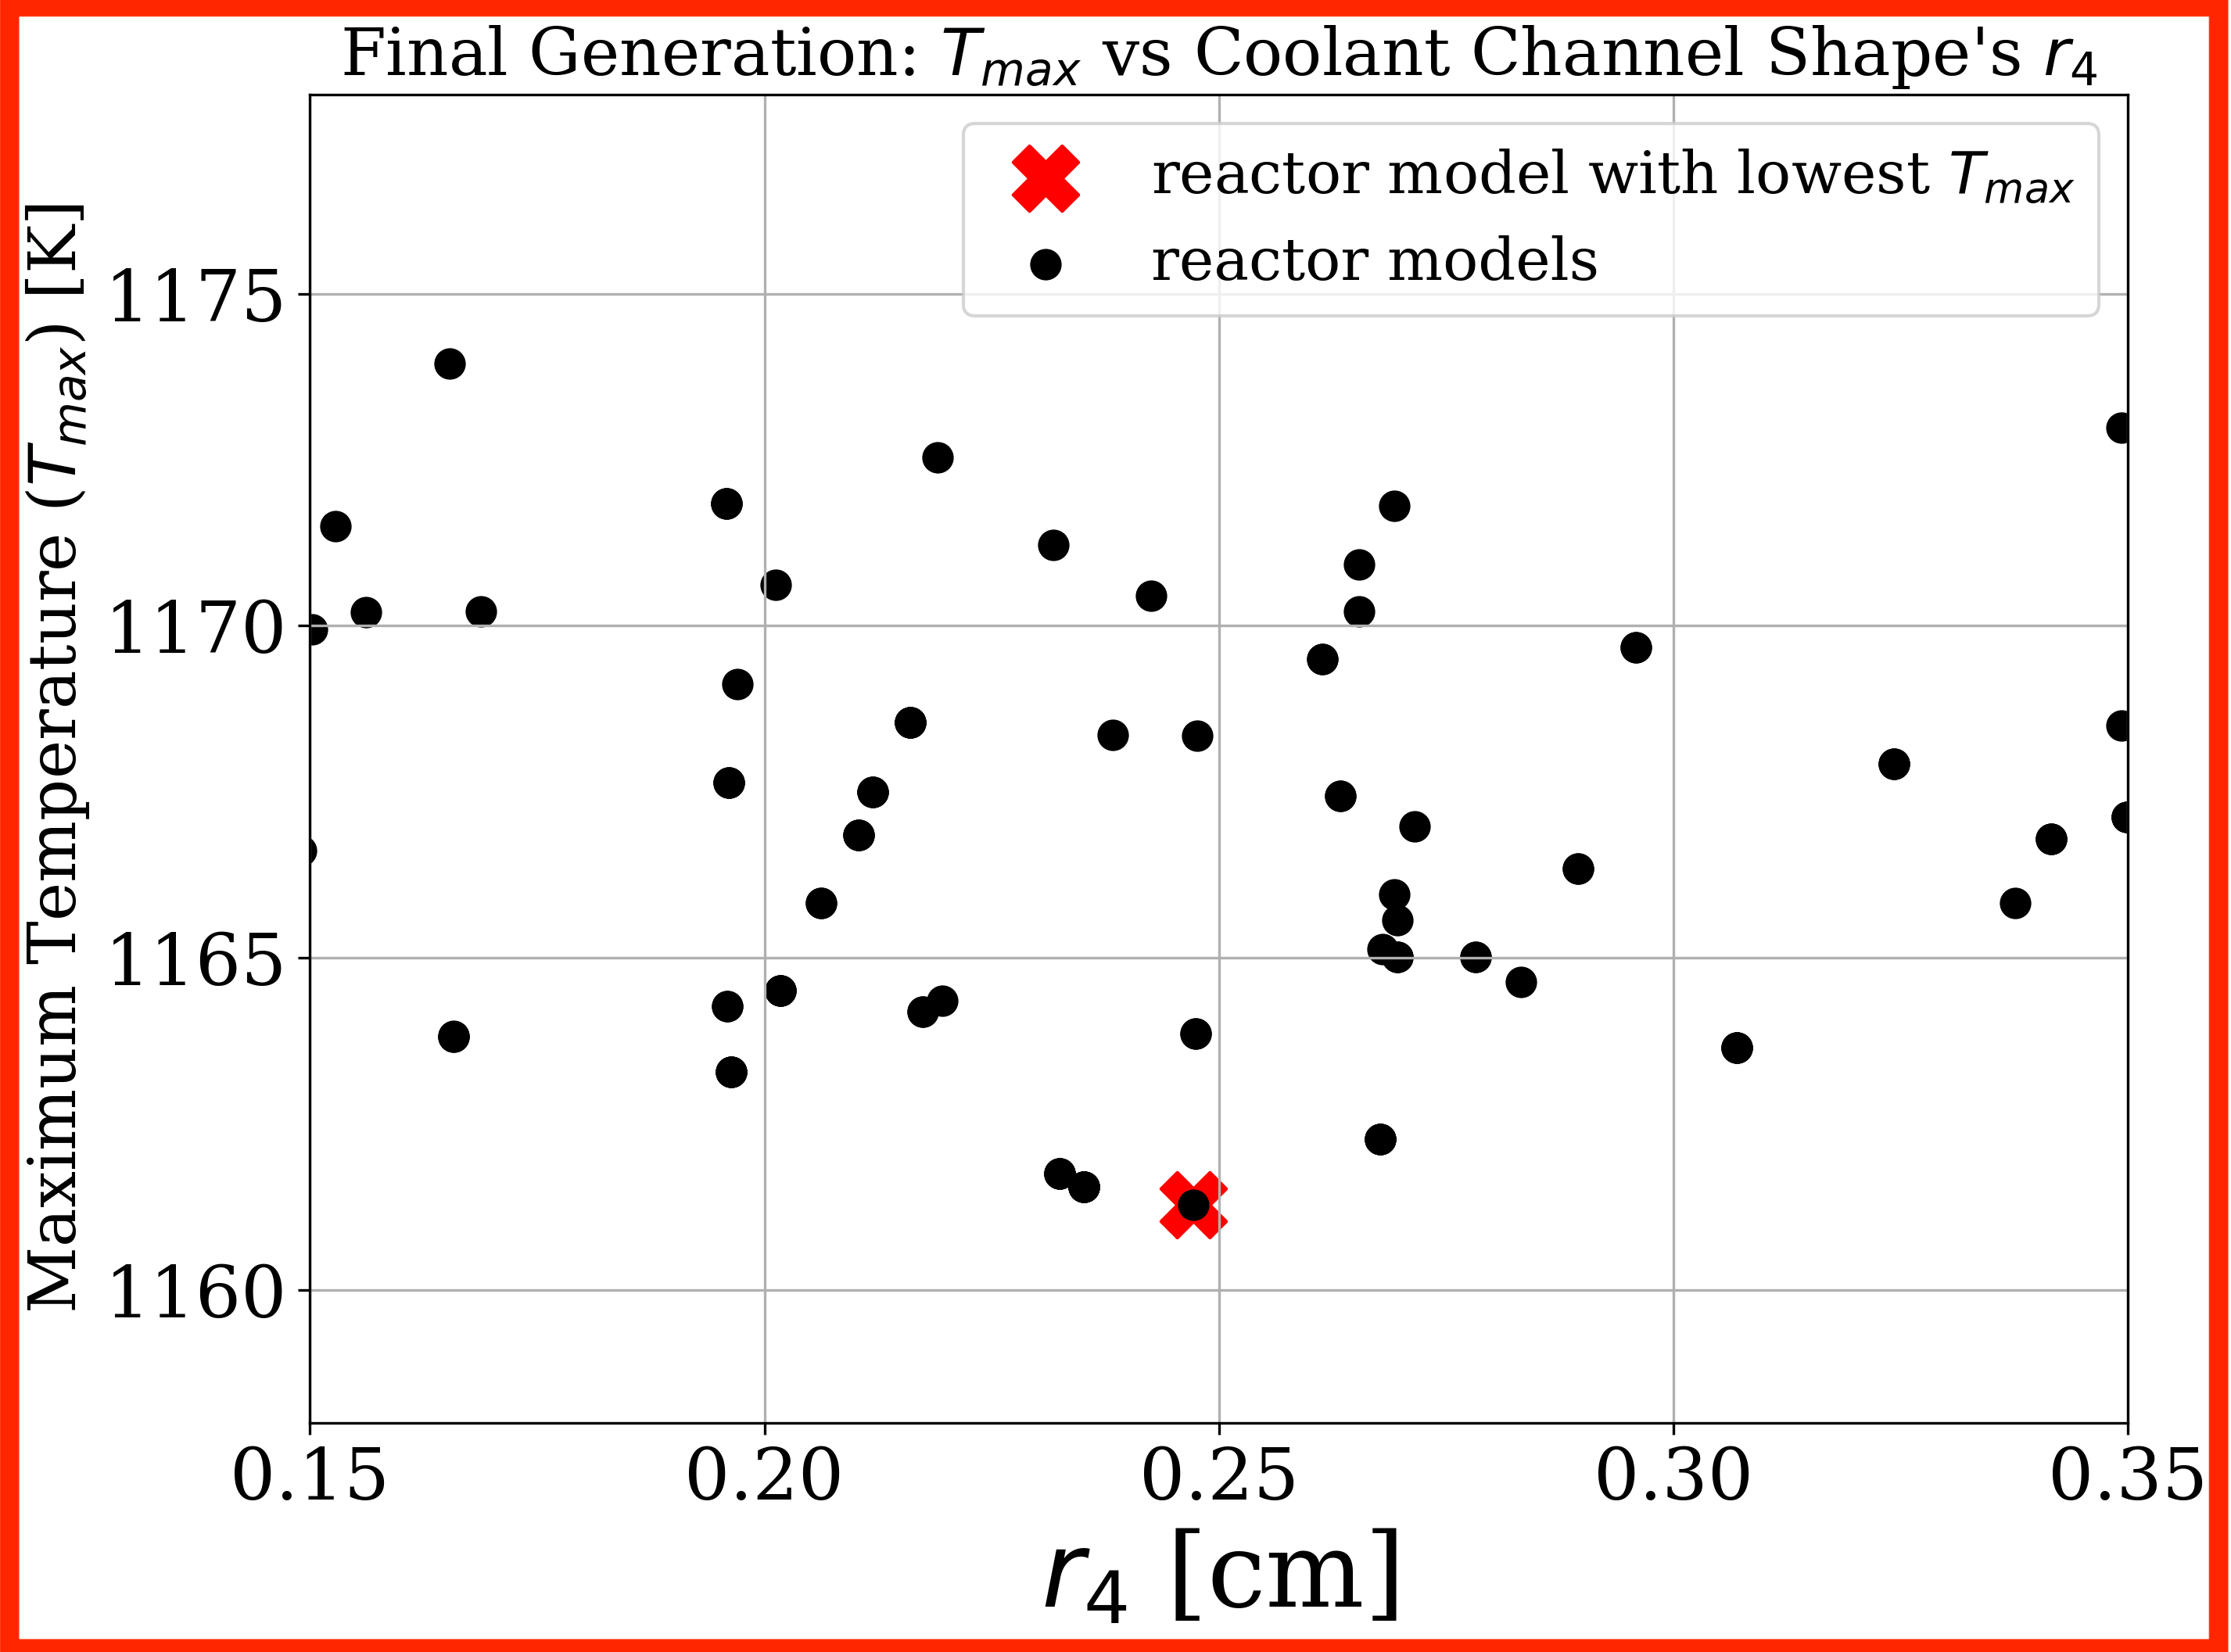
\includegraphics[width=\linewidth]{figures/a-1e-r4-pres-annotated.png}}
            \vspace{-0.5cm}
            \caption{Plot of $T_{max}$ against $r_4$.}
        \end{subfigure}
        \begin{subfigure}{0.3\textwidth}
            \only<1,3>{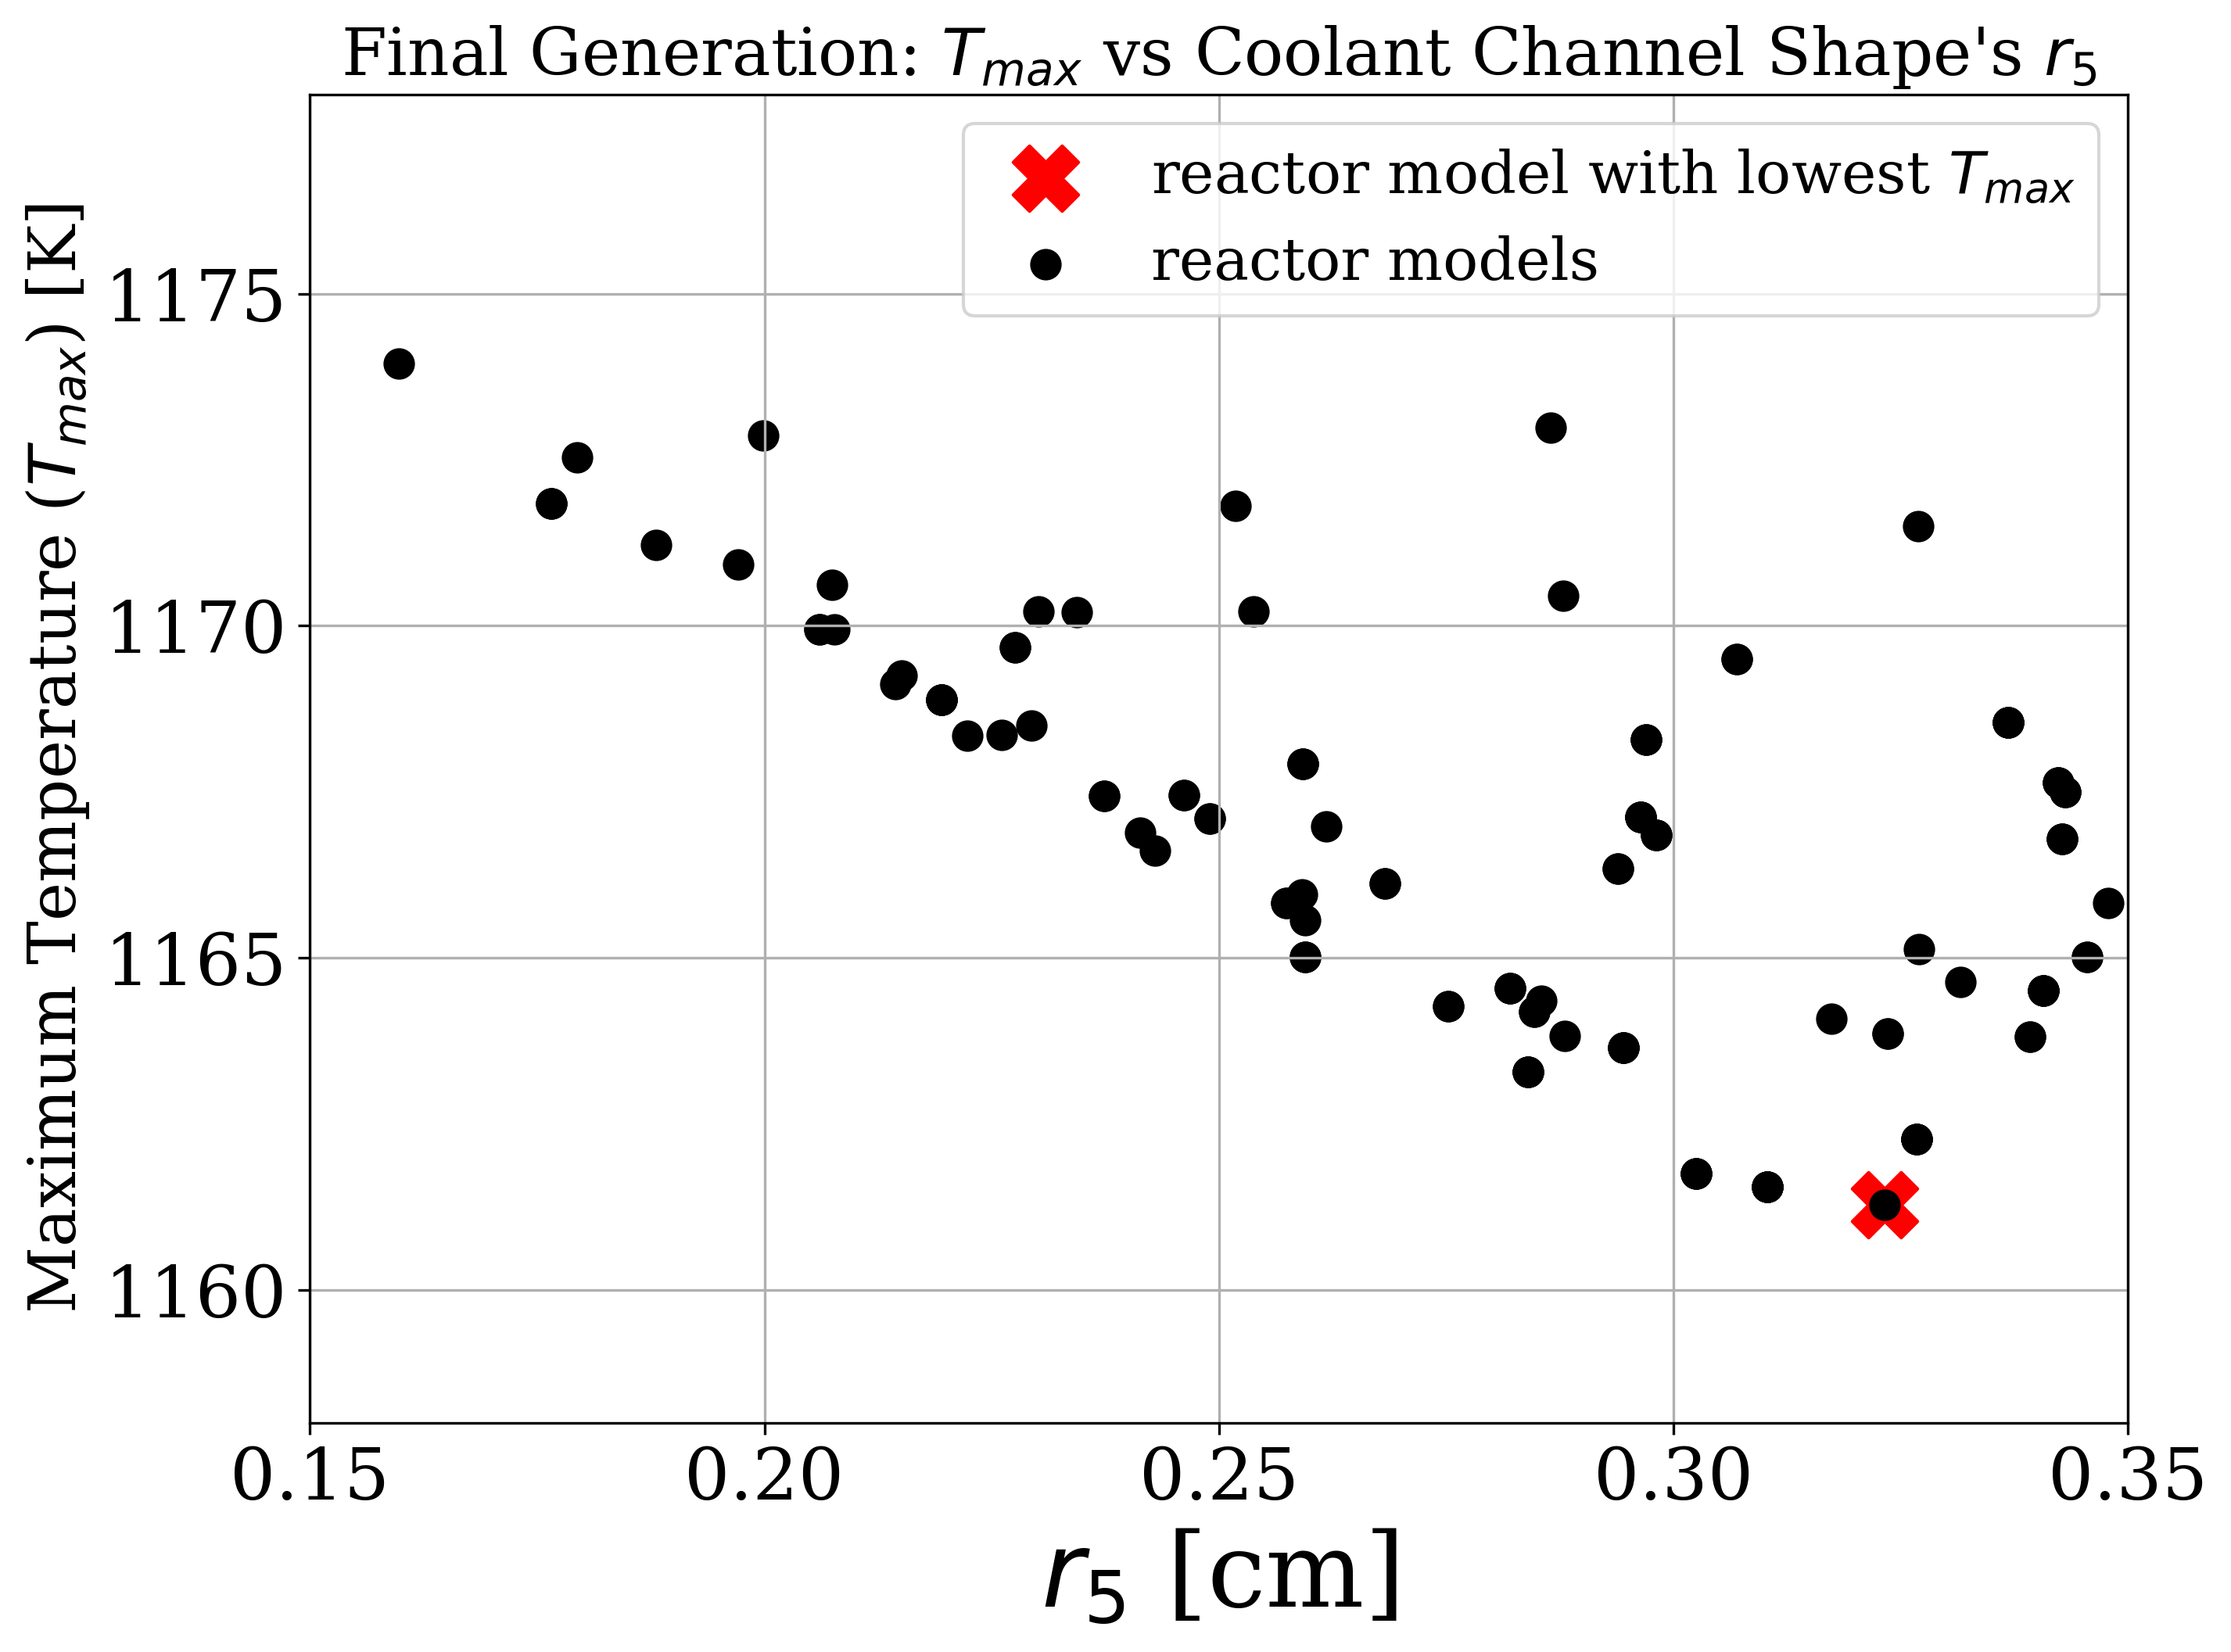
\includegraphics[width=\linewidth]{figures/a-1e-r5-pres.png}}
            \only<2>{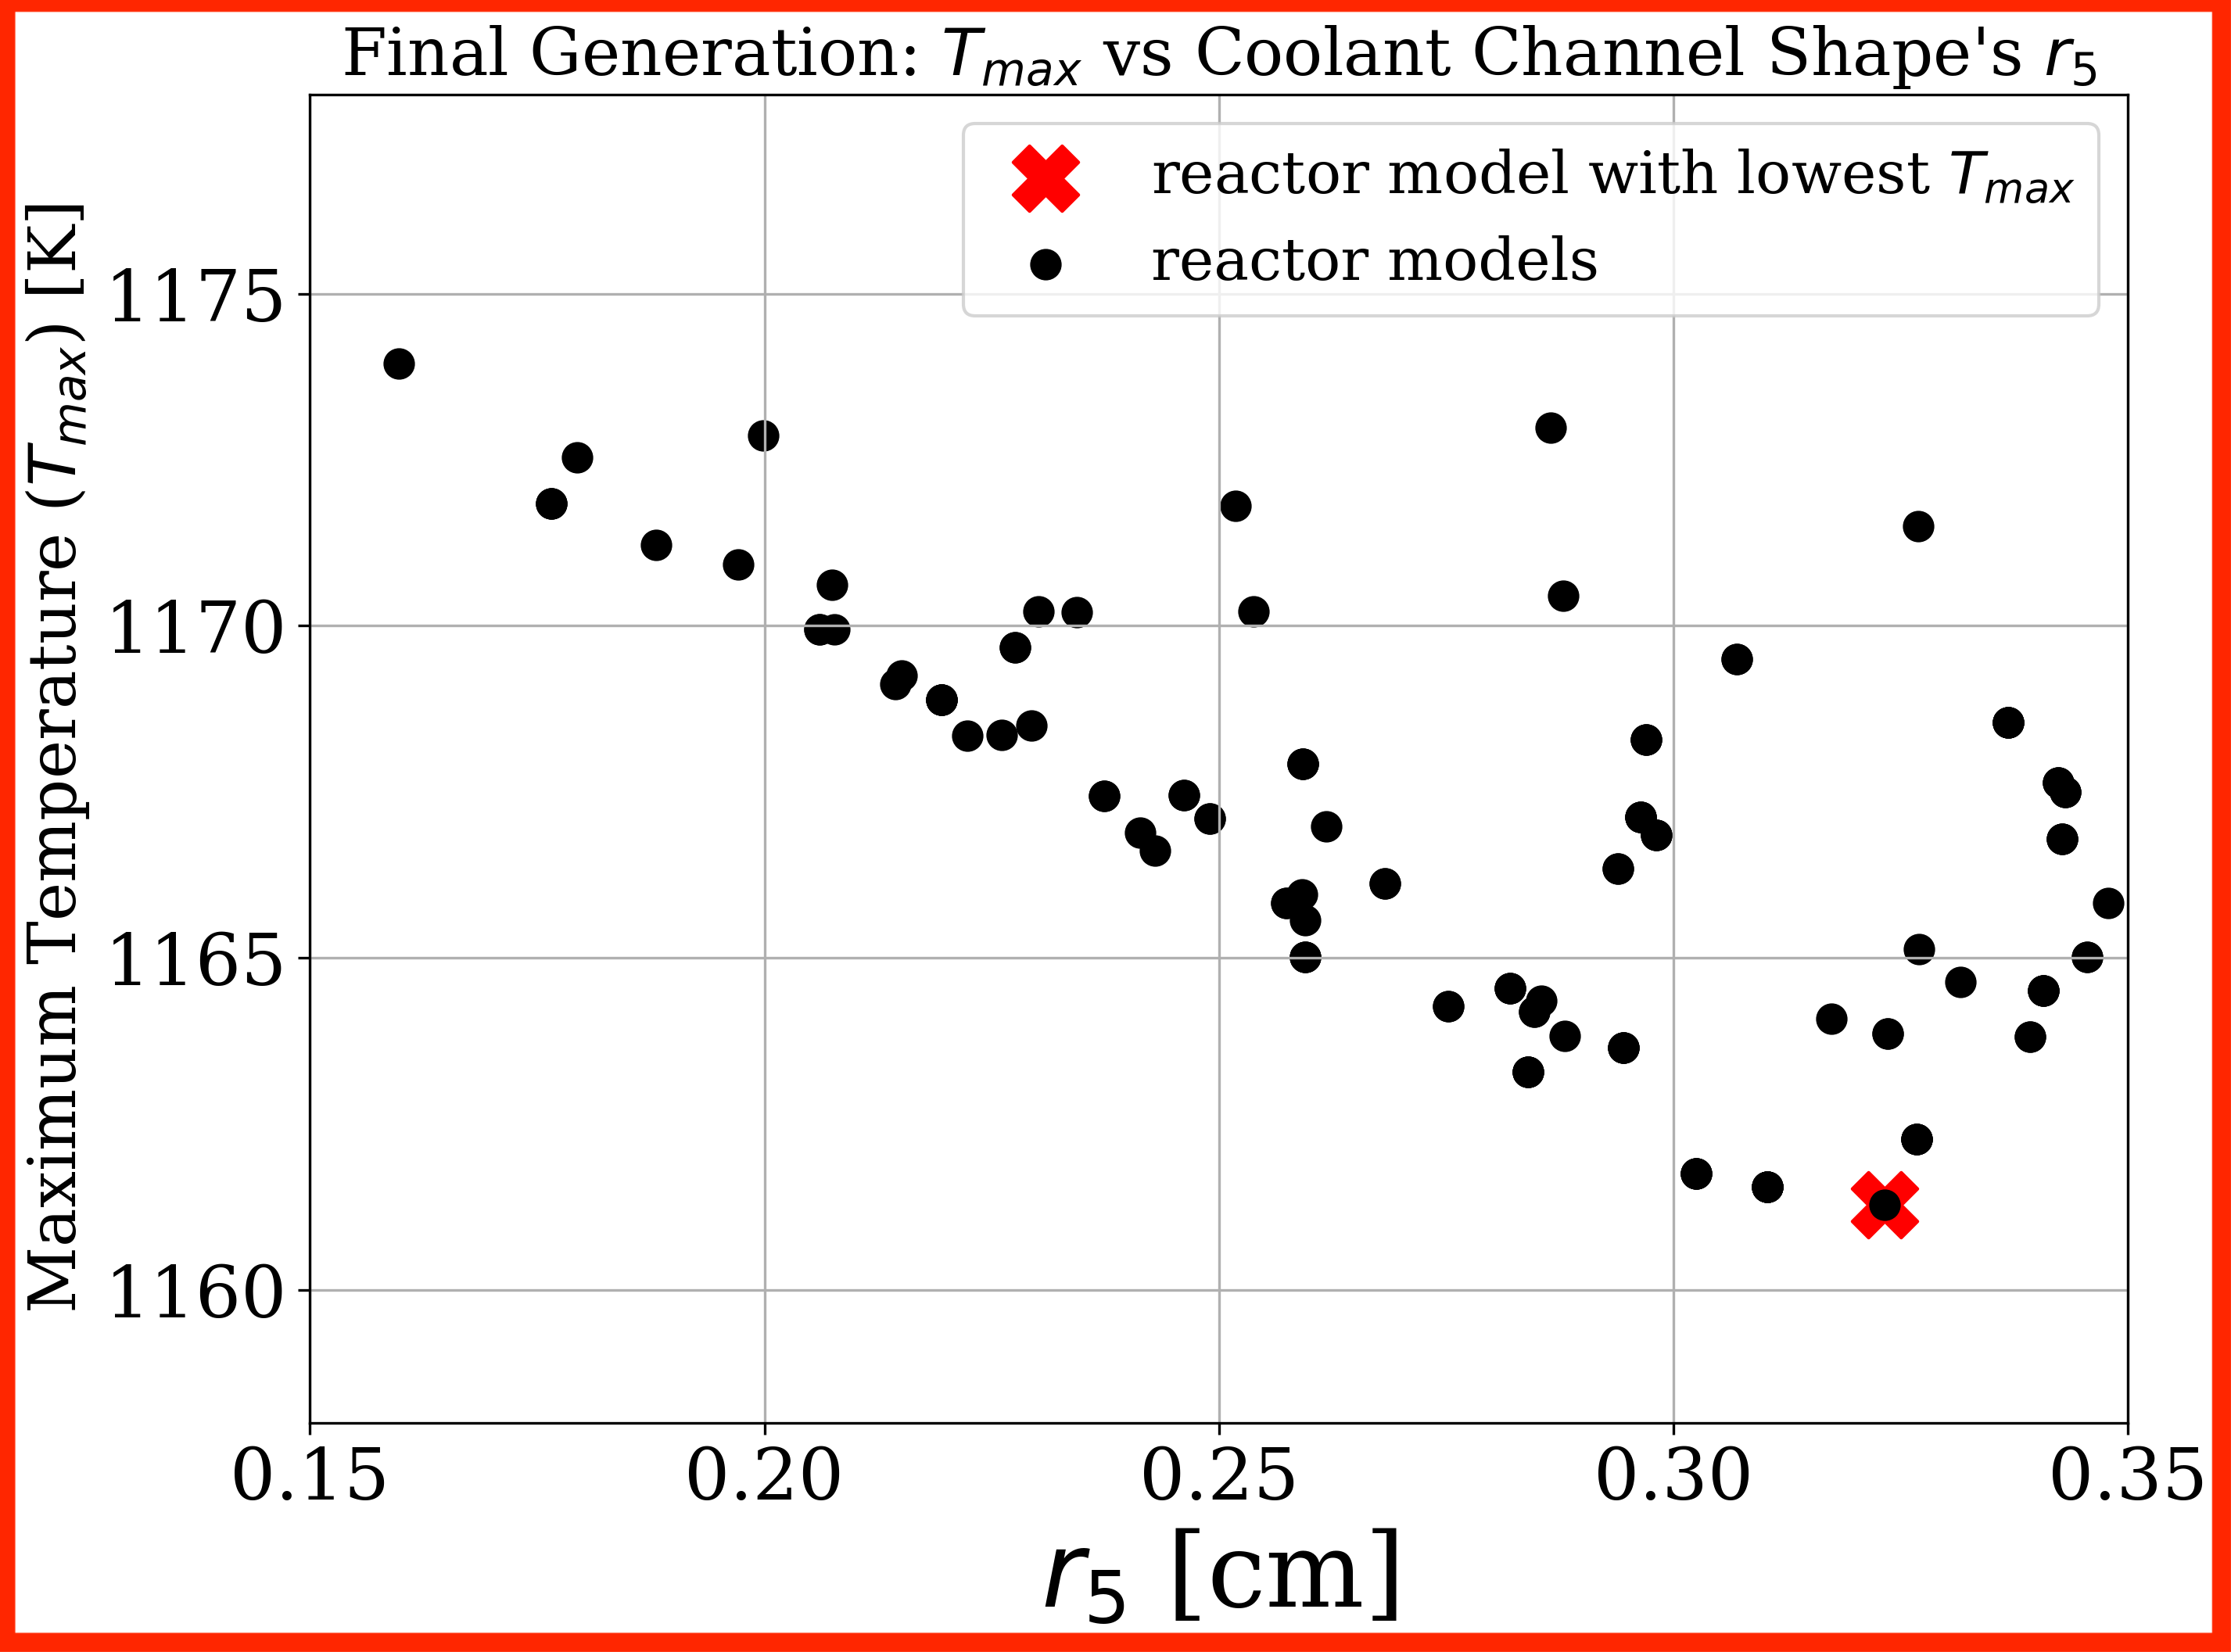
\includegraphics[width=\linewidth]{figures/a-1e-r5-pres-annotated.png}}
            \vspace{-0.5cm}
            \caption{Plot of $T_{max}$ against $r_5$.}
        \end{subfigure}
    \end{figure}
    \only<1>{\textbf{Plots demonstrate if $T_{max}$ is correlated with each radius values.}}
    \only<2>{\textbf{There is a strong negative linear correlation between $T_{max}$ and 
    $r_1$ and $r_5$.}}
    \only<3>{\textbf{Random scattering shows that $T_{max}$ has a weak correlation with 
    $r_2$, $r_3$, $r_4$}.}
\end{frame}

\begin{frame}
    \frametitle{AHTR One-Third Assembly Simulation a-1e Results}
    \begin{figure}
        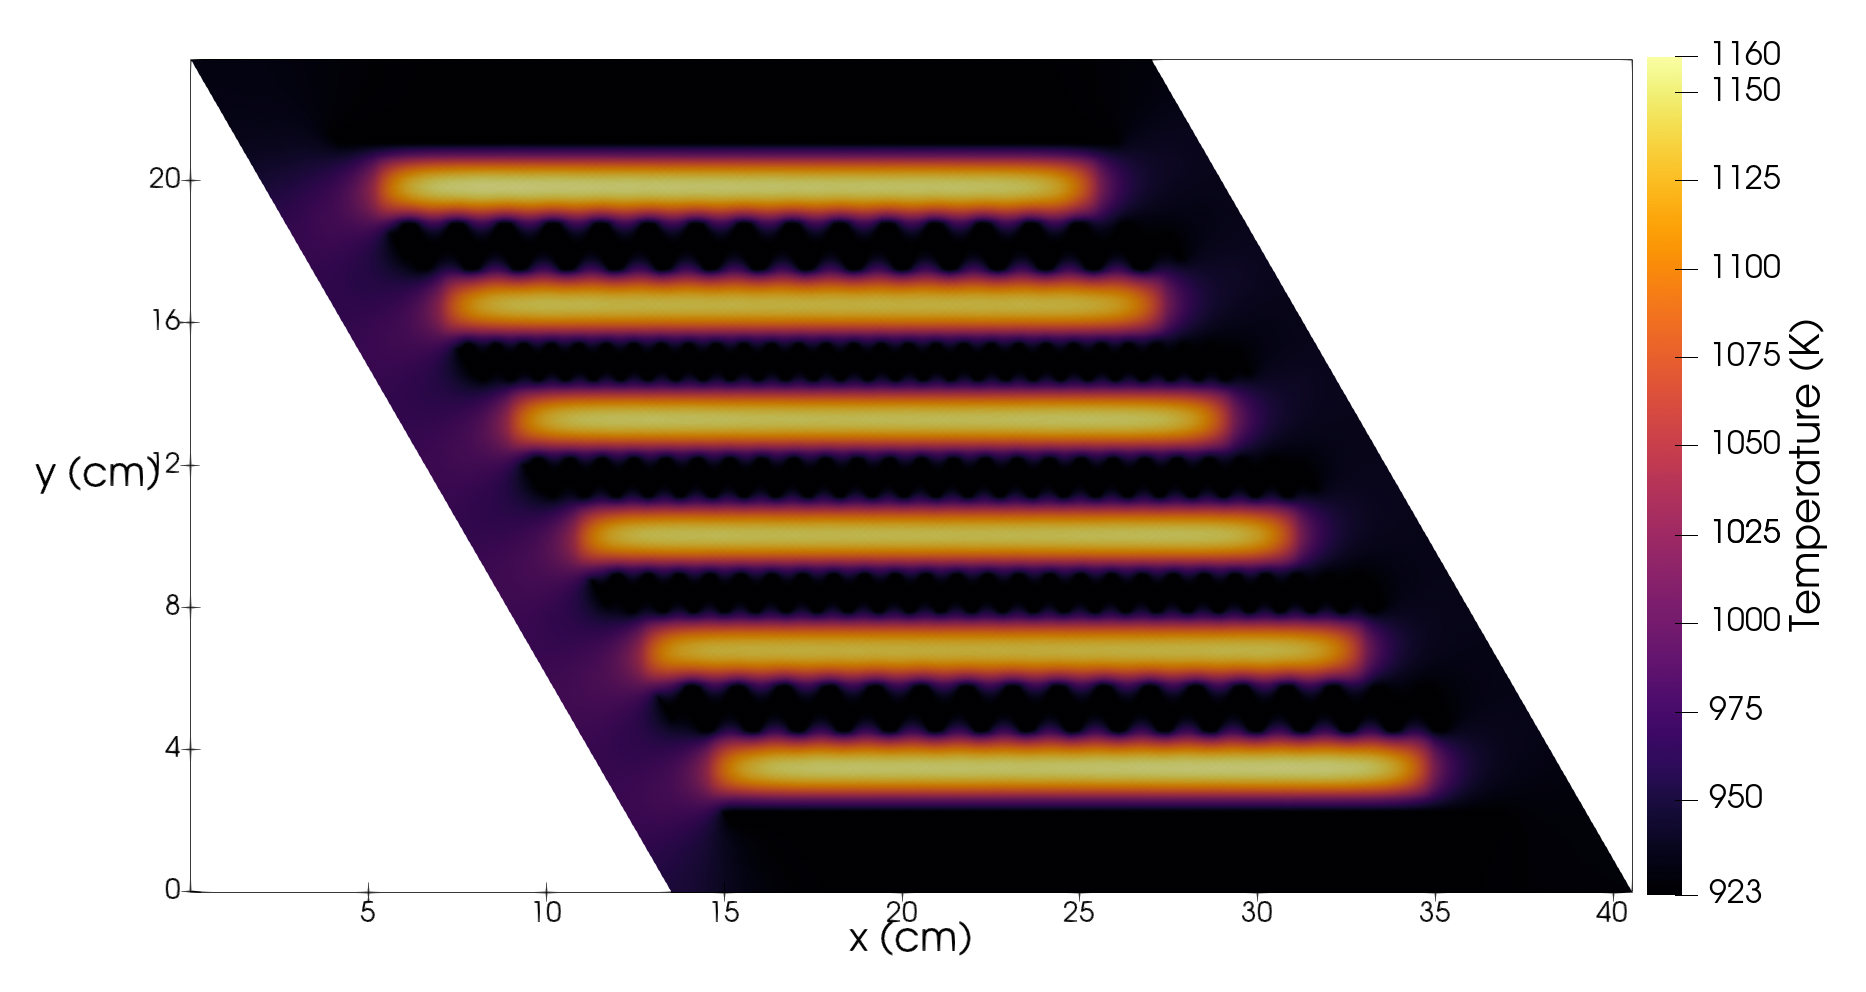
\includegraphics[width=0.59\linewidth]{../docs/figures/a-1e-temp-distribution-2d.png} 
        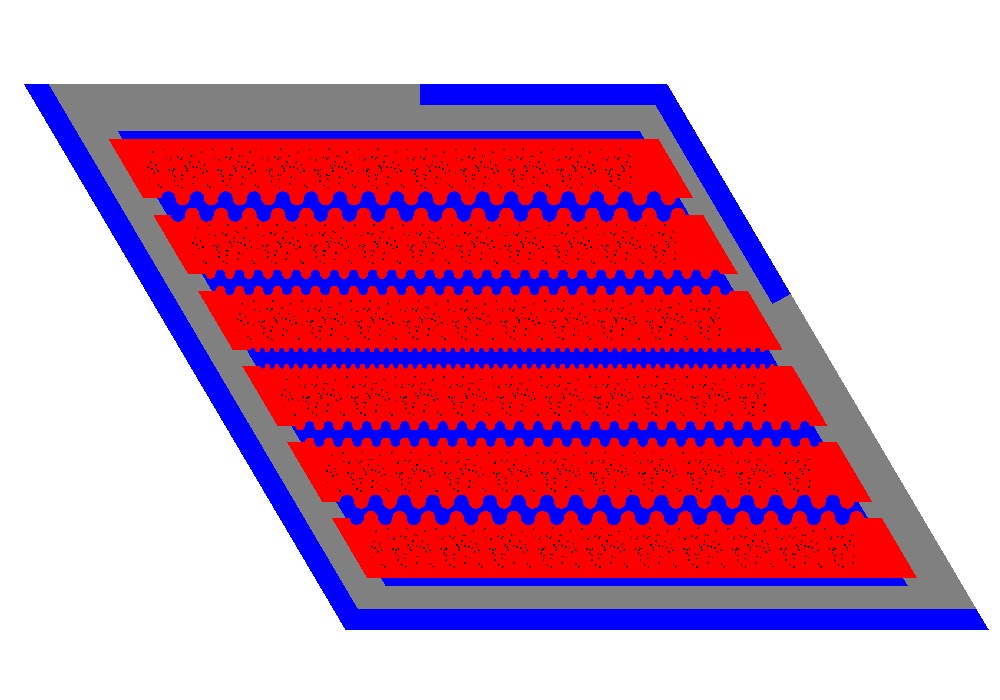
\includegraphics[width=0.4\linewidth]{../docs/figures/coolant-channel-shape-assem.png} 
        \caption{Temperature Distribution in the reactor model with the lowest $T_{max}$.}
    \end{figure}

    To minimize $T_{max}$, ROLLO maximized $r_1$ and $r_5$ to enable enhanced cooling 
    in the top and bottom planks where the temperature peaking was occurring.

    \visible<2->{\begin{tcolorbox}[colback=illiniorange,colframe=illiniorange!50!black]
    \textbf{FLiBe channels located closest to temperature peaks shows a \\ negative 
    correlation with $T_{max}$.}
    \end{tcolorbox}}
\end{frame}

\begin{frame}
    \frametitle{Single-Objective Optimization Major Takeaways}
    \visible<1->{\textbf{Minimize $PF_{total}$ Objective} 
    \begin{itemize}
        \item Driven by maximizing total fission reaction rate
        \item Influences oscillations in TRISO's spatial distribution
        \item No correlation with coolant channel shape  
    \end{itemize}}

    \vspace{0.2cm}
    \visible<2->{\textbf{Minimize $T_{max}$ Objective}
    \begin{itemize}
        \item The minimize $T_{max}$ objective prefers a flatter TRISO distribution 
        \item FLiBe channels located closest to temperature peaks shows a negative 
        correlation with $T_{max}$
    \end{itemize}}

    \vspace{0.2cm}
    \visible<3->{\textbf{Minimize $PPF_{fuel}$ Objective} 
    \begin{itemize}
        \item Driven by flattening thermal flux distribution
        \item Influences oscillations in TRISO's spatial distribution
        \item No correlation with coolant channel shape  
    \end{itemize}}
\end{frame}

\begin{frame}
    \frametitle{AHTR One-Third Assembly Simulation a-2b Results}
    \begin{columns}[t]
        \only<1>{\begin{column}{0.35\textwidth}
        \begin{block}{Simulation a-2b}
        \begin{itemize}
        \item I vary $PF_{total}$ and \textbf{a, b, c, d, e f} 
        ($\rho_{TRISO}(\vec{x}, \vec{y}$)) 
        \item Minimize $PF_{total}$ and $PPF_{fuel}$ objectives
        \item 5 generations 
        \item 128 reactor models per gen  
        \item Total runtime: 492 Theta node-hours
        \end{itemize}
        \end{block}
        \end{column}}
        \only<2>{\begin{column}{0.5\textwidth}
            \begin{block}{Pareto Front}
            \begin{itemize}
                \item Multi objective optimization with competing objectives will return 
                \textbf{multiple optimal solutions that meet each objective to varying 
                degrees}
                \item For each reactor model on the Pareto front, \textbf{none of the 
                objective values can be improved without degrading another}
            \end{itemize}
        \end{block}
        \end{column}}
        \only<3>{\begin{column}{0.35\textwidth}
            \vspace{-0.4cm}
            \begin{block}{Simulation a-2b}
            \begin{itemize}
            \item The 12 reactor models on simulation a-2b's Pareto front have different 
            $PF_{total}$ and $\rho_{TRISO}(\vec{r})$ depending on \textbf{extent each
            objective is minimized.}
            \item Reactor 11 = lowest $PF_{total}$, highest $PPF_{fuel}$
            \item Reactor 3 = lowest $PPF_{fuel}$, highest $PF_{total}$
            \item Reactor 5 = minimizes both objectives equally
            \end{itemize}
            \end{block}
            \end{column}}
    \only<1,3>{    
        \begin{column}{0.65\textwidth}
        \textbf{Simulation a-2b's Pareto front shows the tradeoff between 
        minimize $PF_{total}$ and $PPF_{fuel}$ objectives.}
        \begin{figure}
            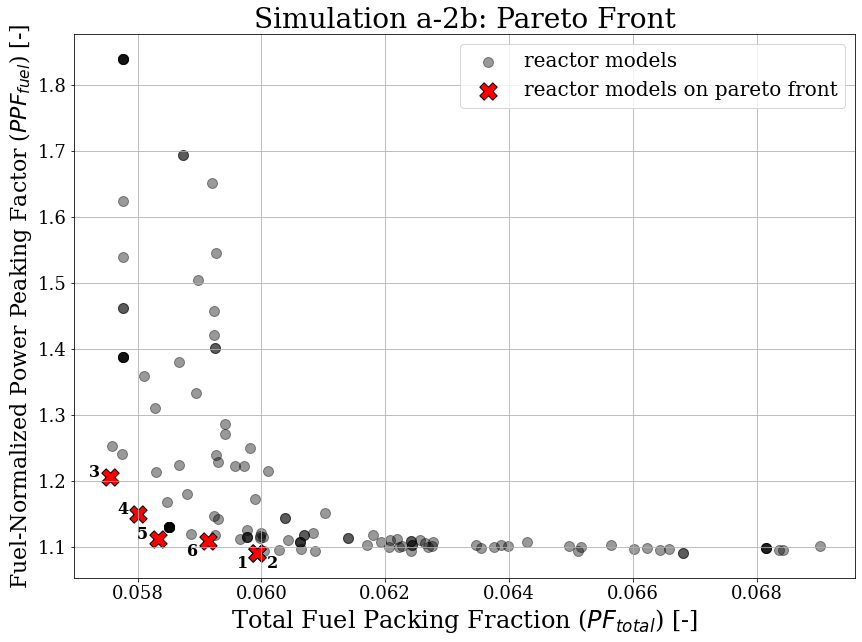
\includegraphics[width=\linewidth]{../docs/figures/assem-obj-2-pfppf-pareto.png} 
        \end{figure}
    \end{column}}
    \only<2>{    
        \begin{column}{0.5\textwidth}
        \begin{figure}
            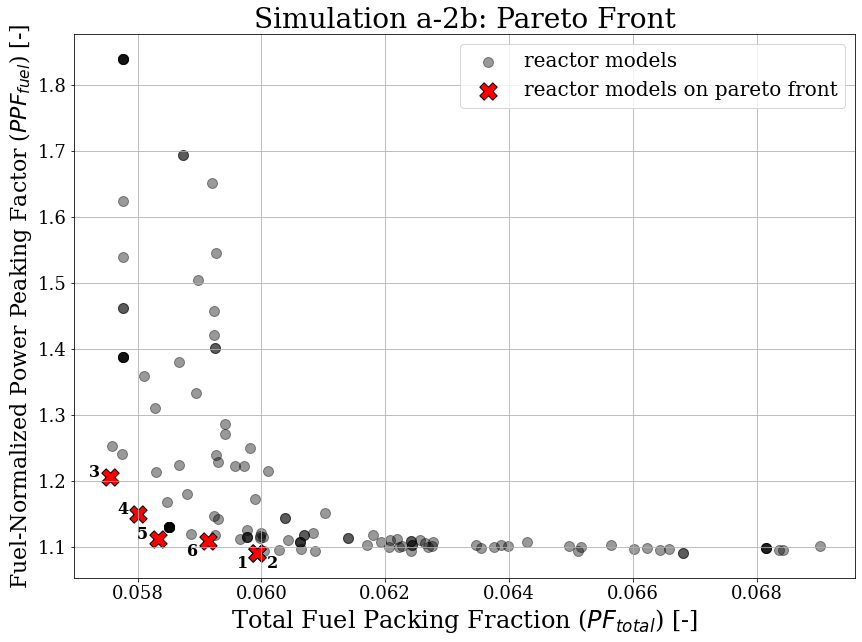
\includegraphics[width=\linewidth]{../docs/figures/assem-obj-2-pfppf-pareto.png} 
        \end{figure}
    \end{column}}
    \end{columns}

    \vspace{0.4cm}
    \only<2>{\textbf{Successful multi-objective optimization finds a wide spread of 
    reactor models on their Pareto fronts}}
\end{frame}

\begin{frame}
    \frametitle{AHTR One-Third Assembly Simulation a-2b Results}
    \centering
    \textbf{ROLLO found a wide variety of TRISO distributions on the Pareto front 
    that minimize each objective to a different extent.}

    \vspace{0.2cm}
    \begin{figure}
        \only<1>{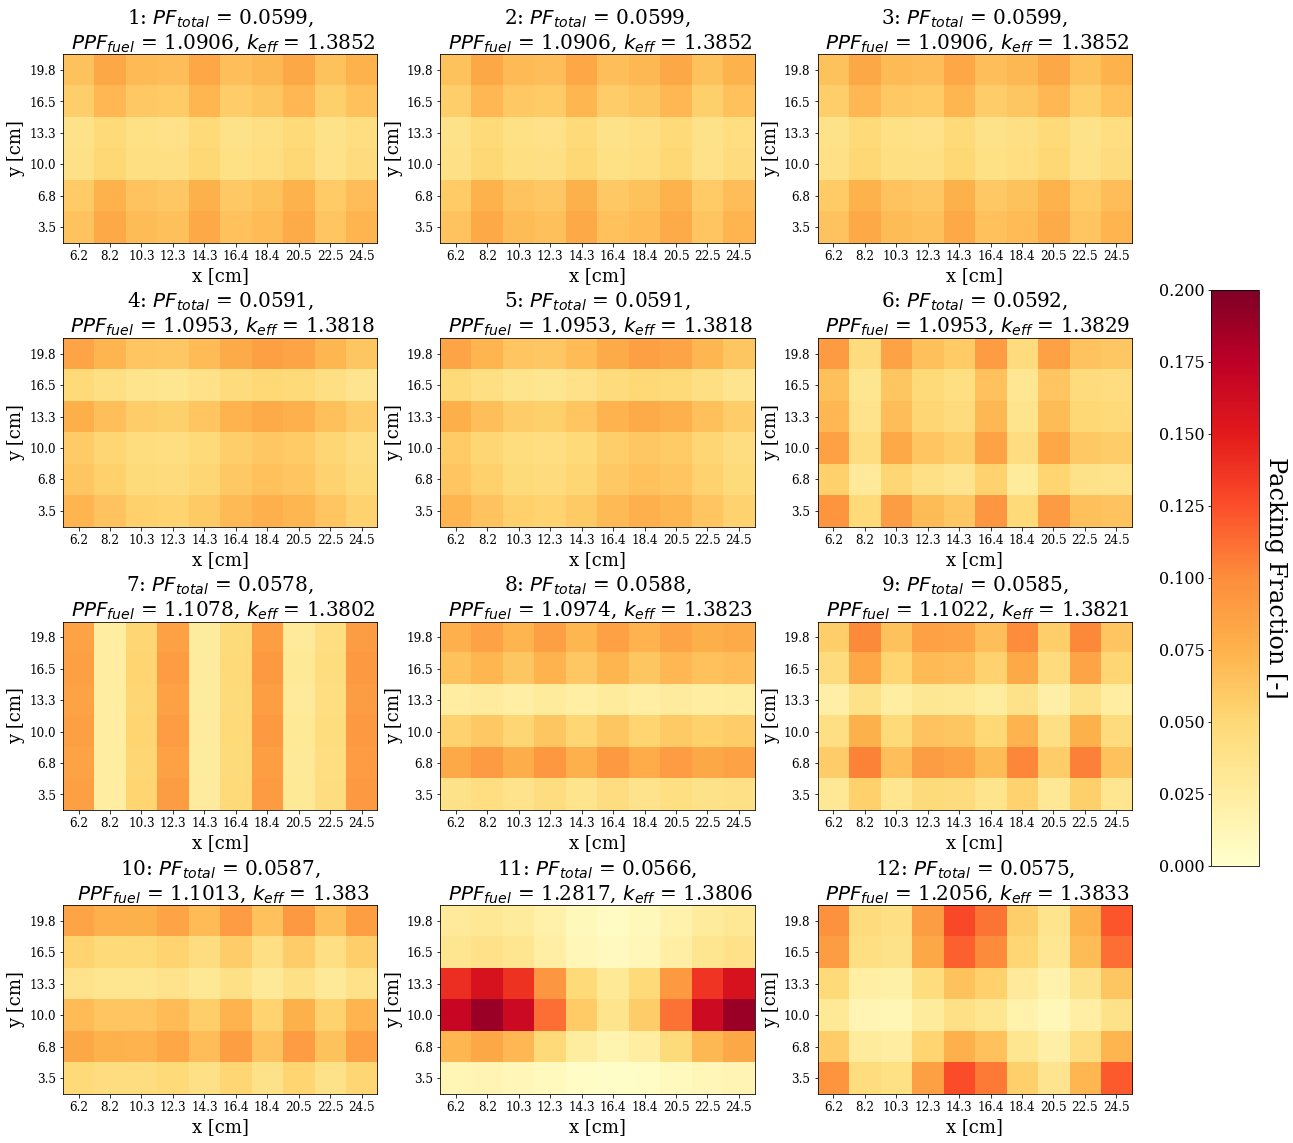
\includegraphics[width=0.8\linewidth]{../docs/figures/assem-obj-2-pfppf-pareto-distr.png}}
        \only<2>{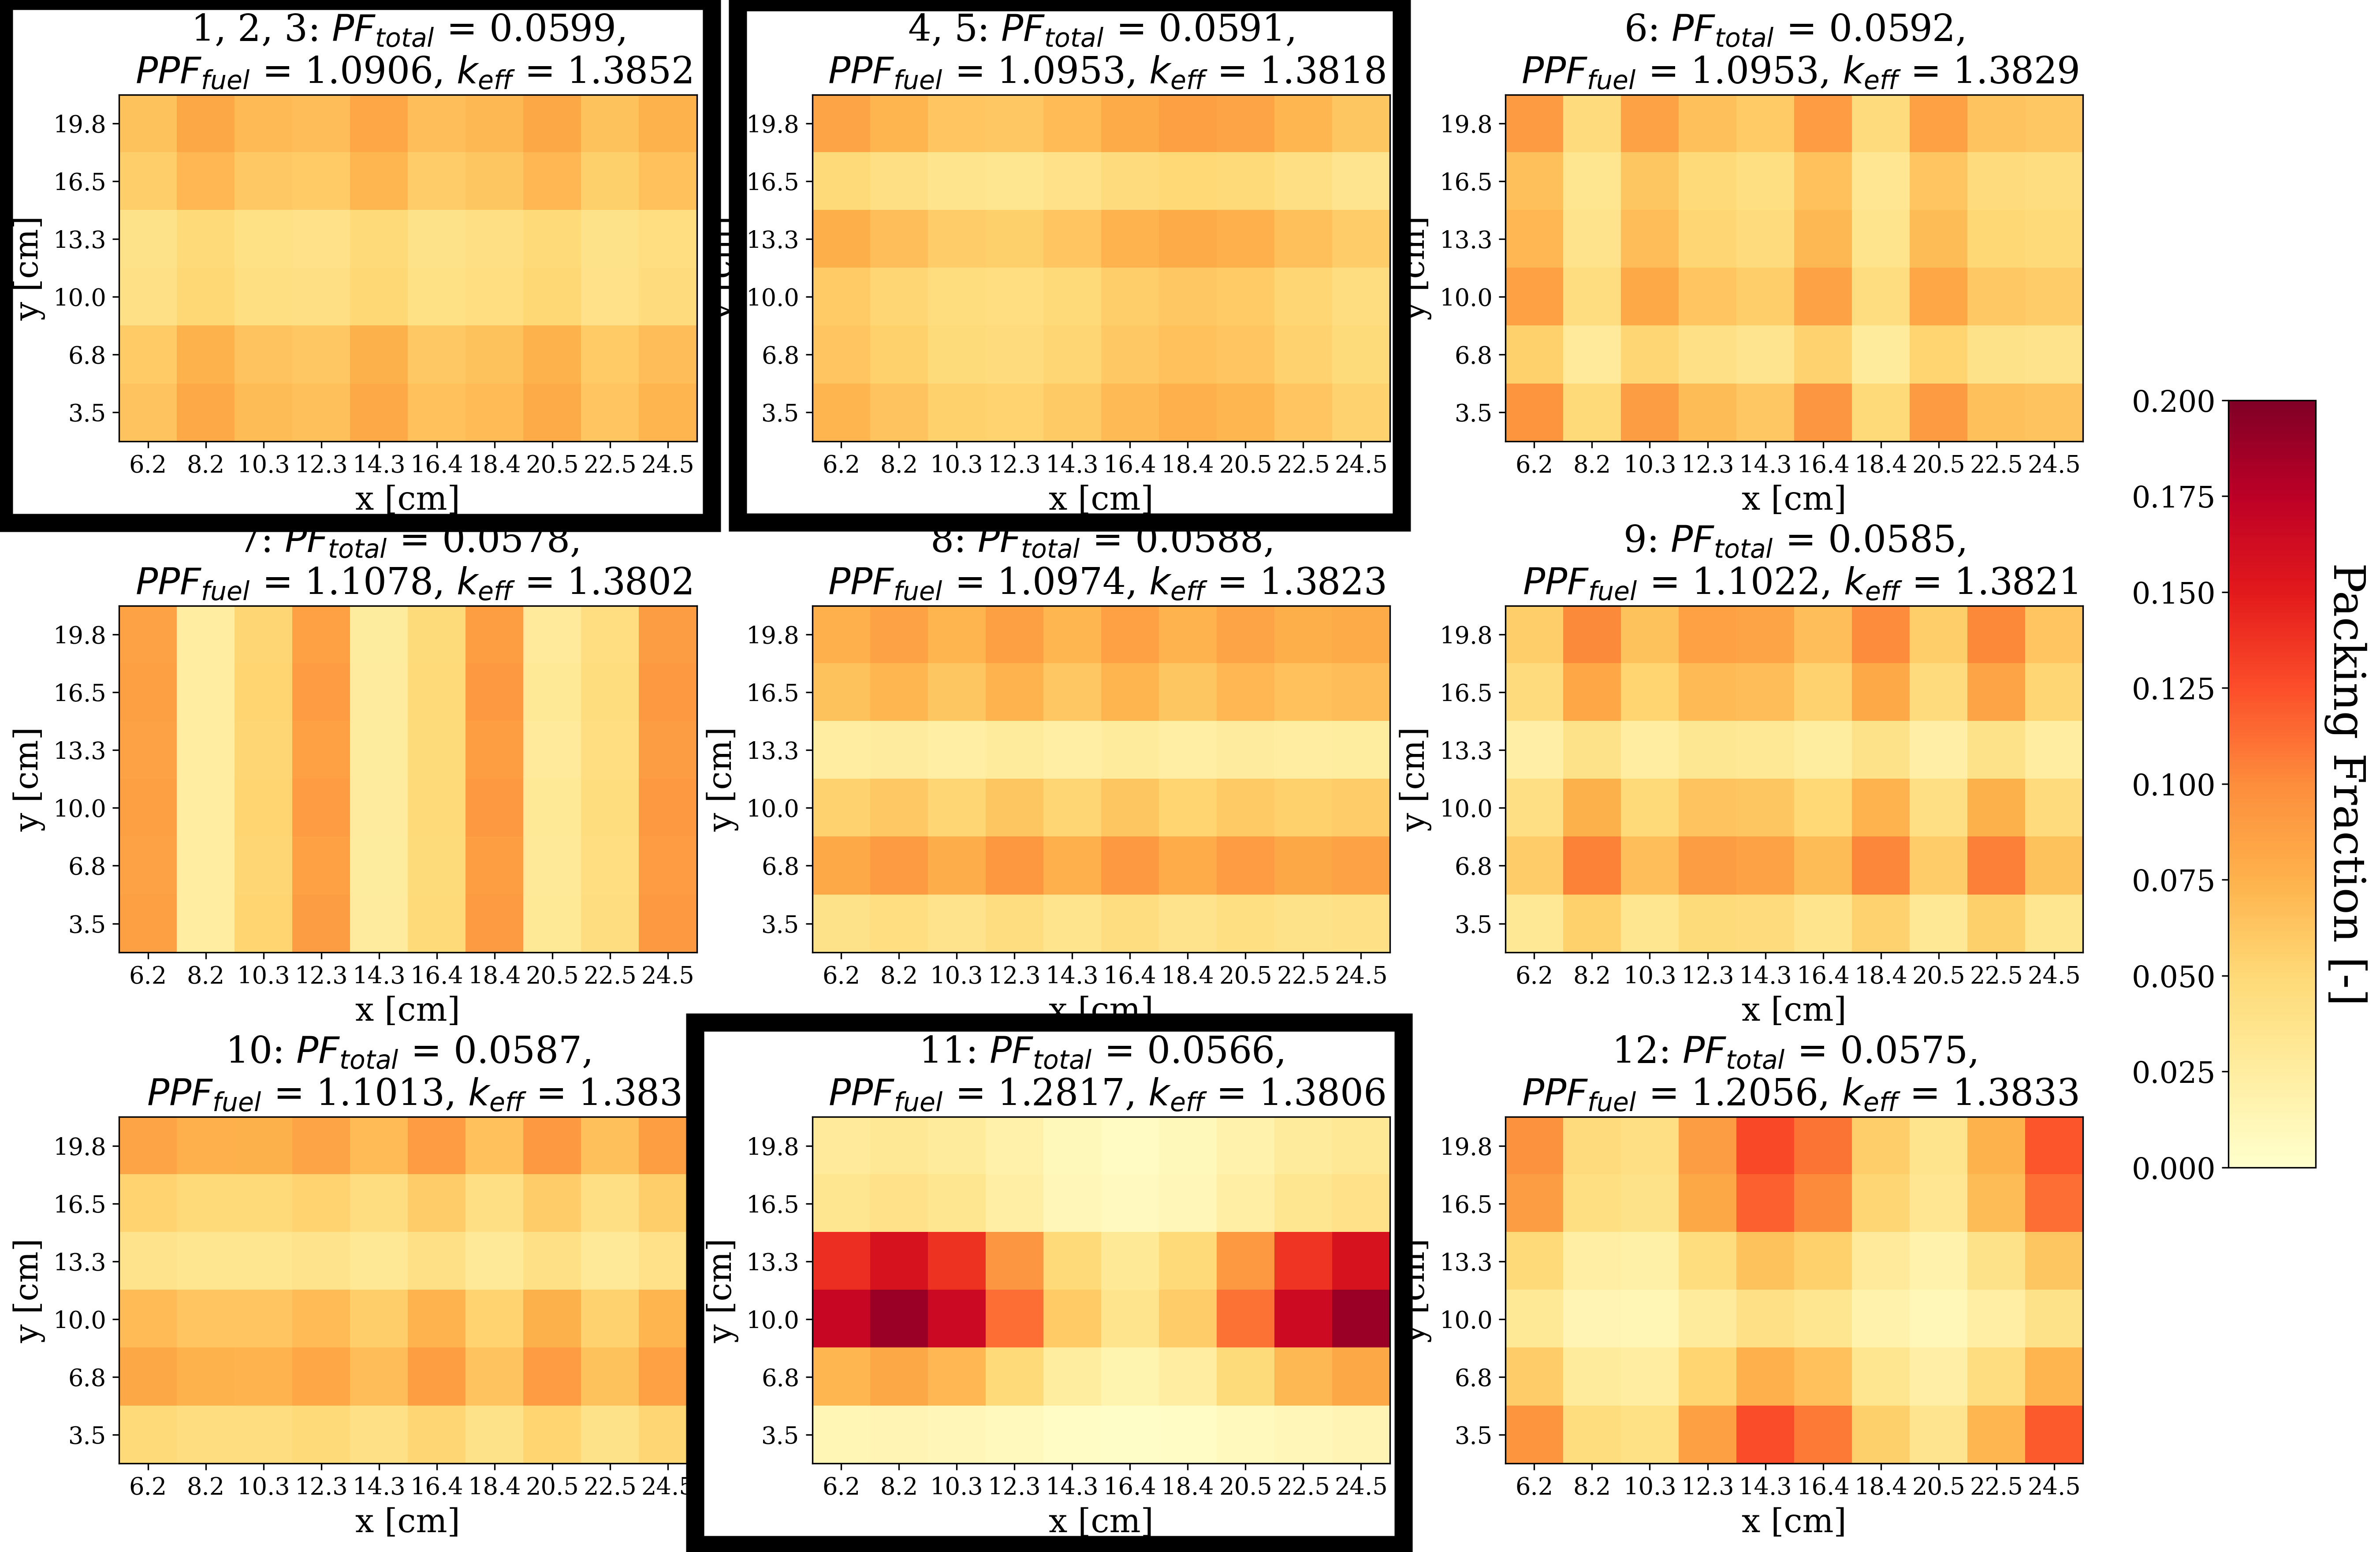
\includegraphics[width=0.8\linewidth]{figures/assem-obj-2-pfppf-pareto-distr-annotated.png}}
    \end{figure}
\end{frame}

\begin{frame}
    \frametitle{AHTR One-Third Assembly Simulation a-2b Results}
    \begin{figure}
        \centering
        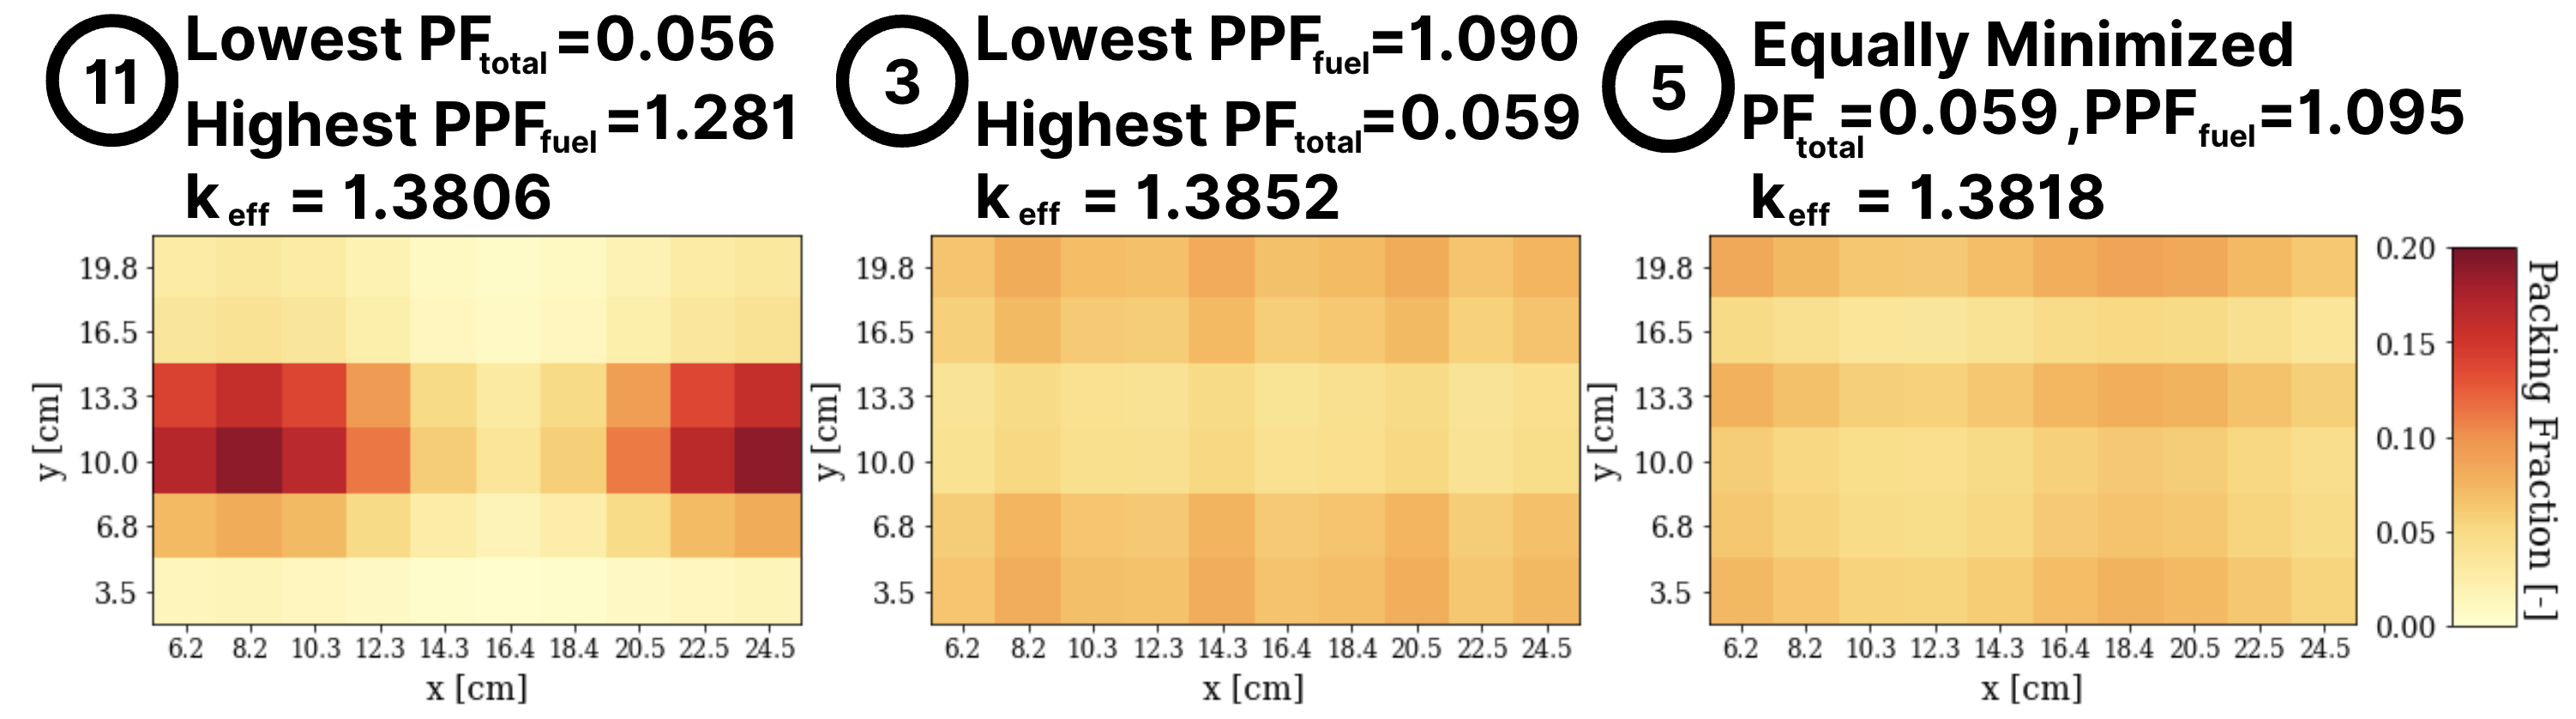
\includegraphics[width=\linewidth]{figures/a-2b-comparison-reactors.png}
    \end{figure}

    Minimize $PF_{total}$ is driven by \textbf{maximizing total fission reaction rate} 
    \begin{itemize}
        \visible<1->{\item Reactor 11 with $PF_{total} = 0.056$ and reactor model 5 with 
        $PF_{total} = 0.059$ have the similar $k_{eff}$ and total fission reaction rate} 
        \visible<2->{\item Reactor 11 TRISO distribution enables it to achieve the 
        same $k_{eff}$ as reactor 5 despite having a lower $PF_{total}$}
        \visible<3->{\item \textbf{Reactor 11 TRISO distribution minimizes spatial 
        self-shielding effects}}
    \end{itemize}
\end{frame}

\begin{frame}
    \frametitle{AHTR One-Third Assembly Simulation a-2b Results}
    \begin{figure}
        \centering
        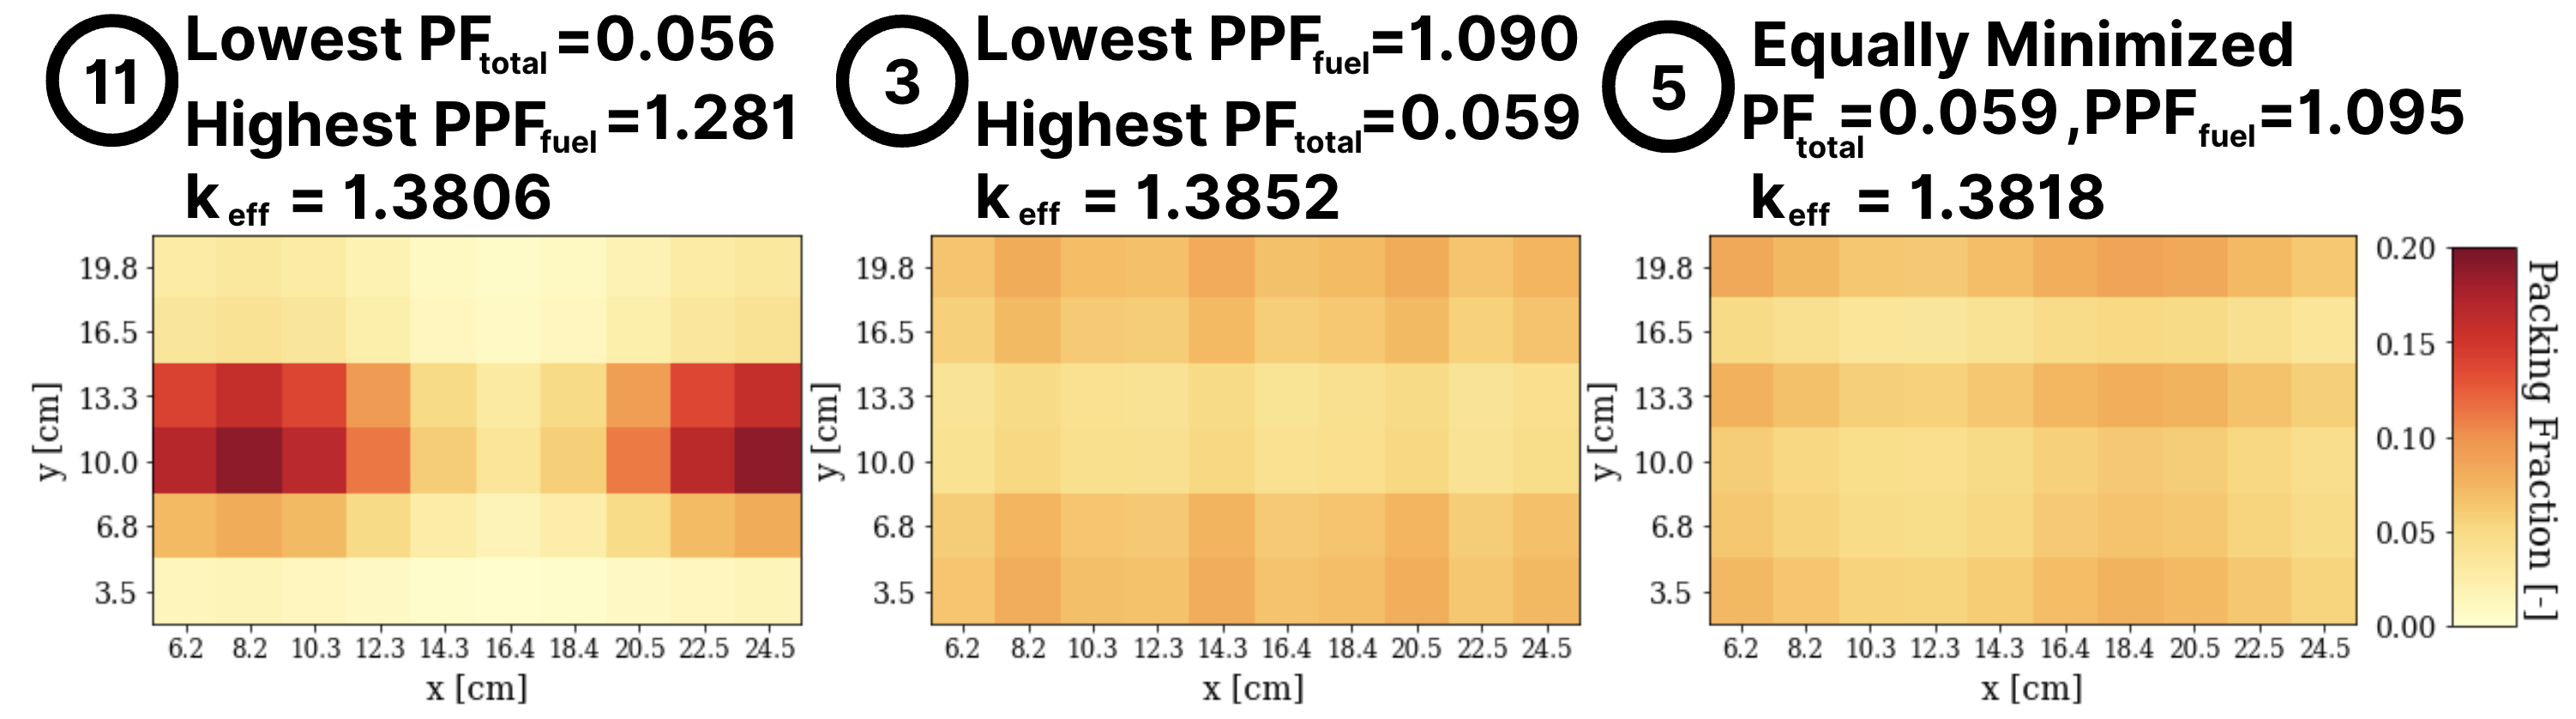
\includegraphics[width=\linewidth]{figures/a-2b-comparison-reactors.png}
    \end{figure}

    Minimize $PPF_{fuel}$ objective is driven by \textbf{flattening thermal 
    flux distribution}  
    \begin{itemize}
        \item Flattest to least flat thermal flux: reactor model 
                $3 \rightarrow 5 \rightarrow 11$
        \item \textbf{Reactor model 3 with lowest $PPF_{fuel}$ has flattest flux}
    \end{itemize}

    \visible<2->{\begin{tcolorbox}[colback=illiniorange,colframe=illiniorange!50!black]
        Minimize $PF_{total}$ and Minimize $PPF_{fuel}$ objectives 
        influence each other resulting in \textbf{unexpected TRISO distributions at 
        different $PF_{total}$ values}. 
    \end{tcolorbox}}
\end{frame}

\begin{frame}
    \frametitle{AHTR One-Third Assembly Simulation a-3b Results}
    \begin{columns}[t]
    \only<1>{\begin{column}{0.35\textwidth}
        \begin{block}{Simulation a-3b}
            \begin{itemize}
            \item Vary $PF_{total}$, \textbf{a, b, c, d, e f} ($\rho_{TRISO}(\vec{x}, 
            \vec{y}$)), and $r_1, r_2, r_3, r_4, r_5$ (coolant channel shape) 
            \item Minimize all three objectives: $PF_{total}$, $T_{max}$ and $PPF_{fuel}$.
            \item 6 generations 
            \item 128 reactor models per gen 
            \item Total runtime: 1528 Theta node-hours 
            \end{itemize}
            \end{block}
        \end{column}}
    \only<2>{\begin{column}{0.4\textwidth}
        \begin{block}{Simulation a-3b}
        \begin{itemize}
        \item The 12 reactor models on simulation a-3b's Pareto front have different 
        input parameters depending on \textbf{extent each
        objective is minimized}
        \item Reactor 11 = lowest $PF_{total}$
        \item Reactor 1 = lowest $T_{max}$
        \item Reactor 4 = lowest $PPF_{fuel}$
        \item Reactor 2 = minimizes all objectives equally
        \end{itemize}
        \end{block}
        \end{column}}

    \begin{column}{0.7\textwidth}
        \only<1>{\textbf{ROLLO successfully found 12 widely spread out reactor models on a-3b's 
        Pareto front.}}
    \begin{figure}
        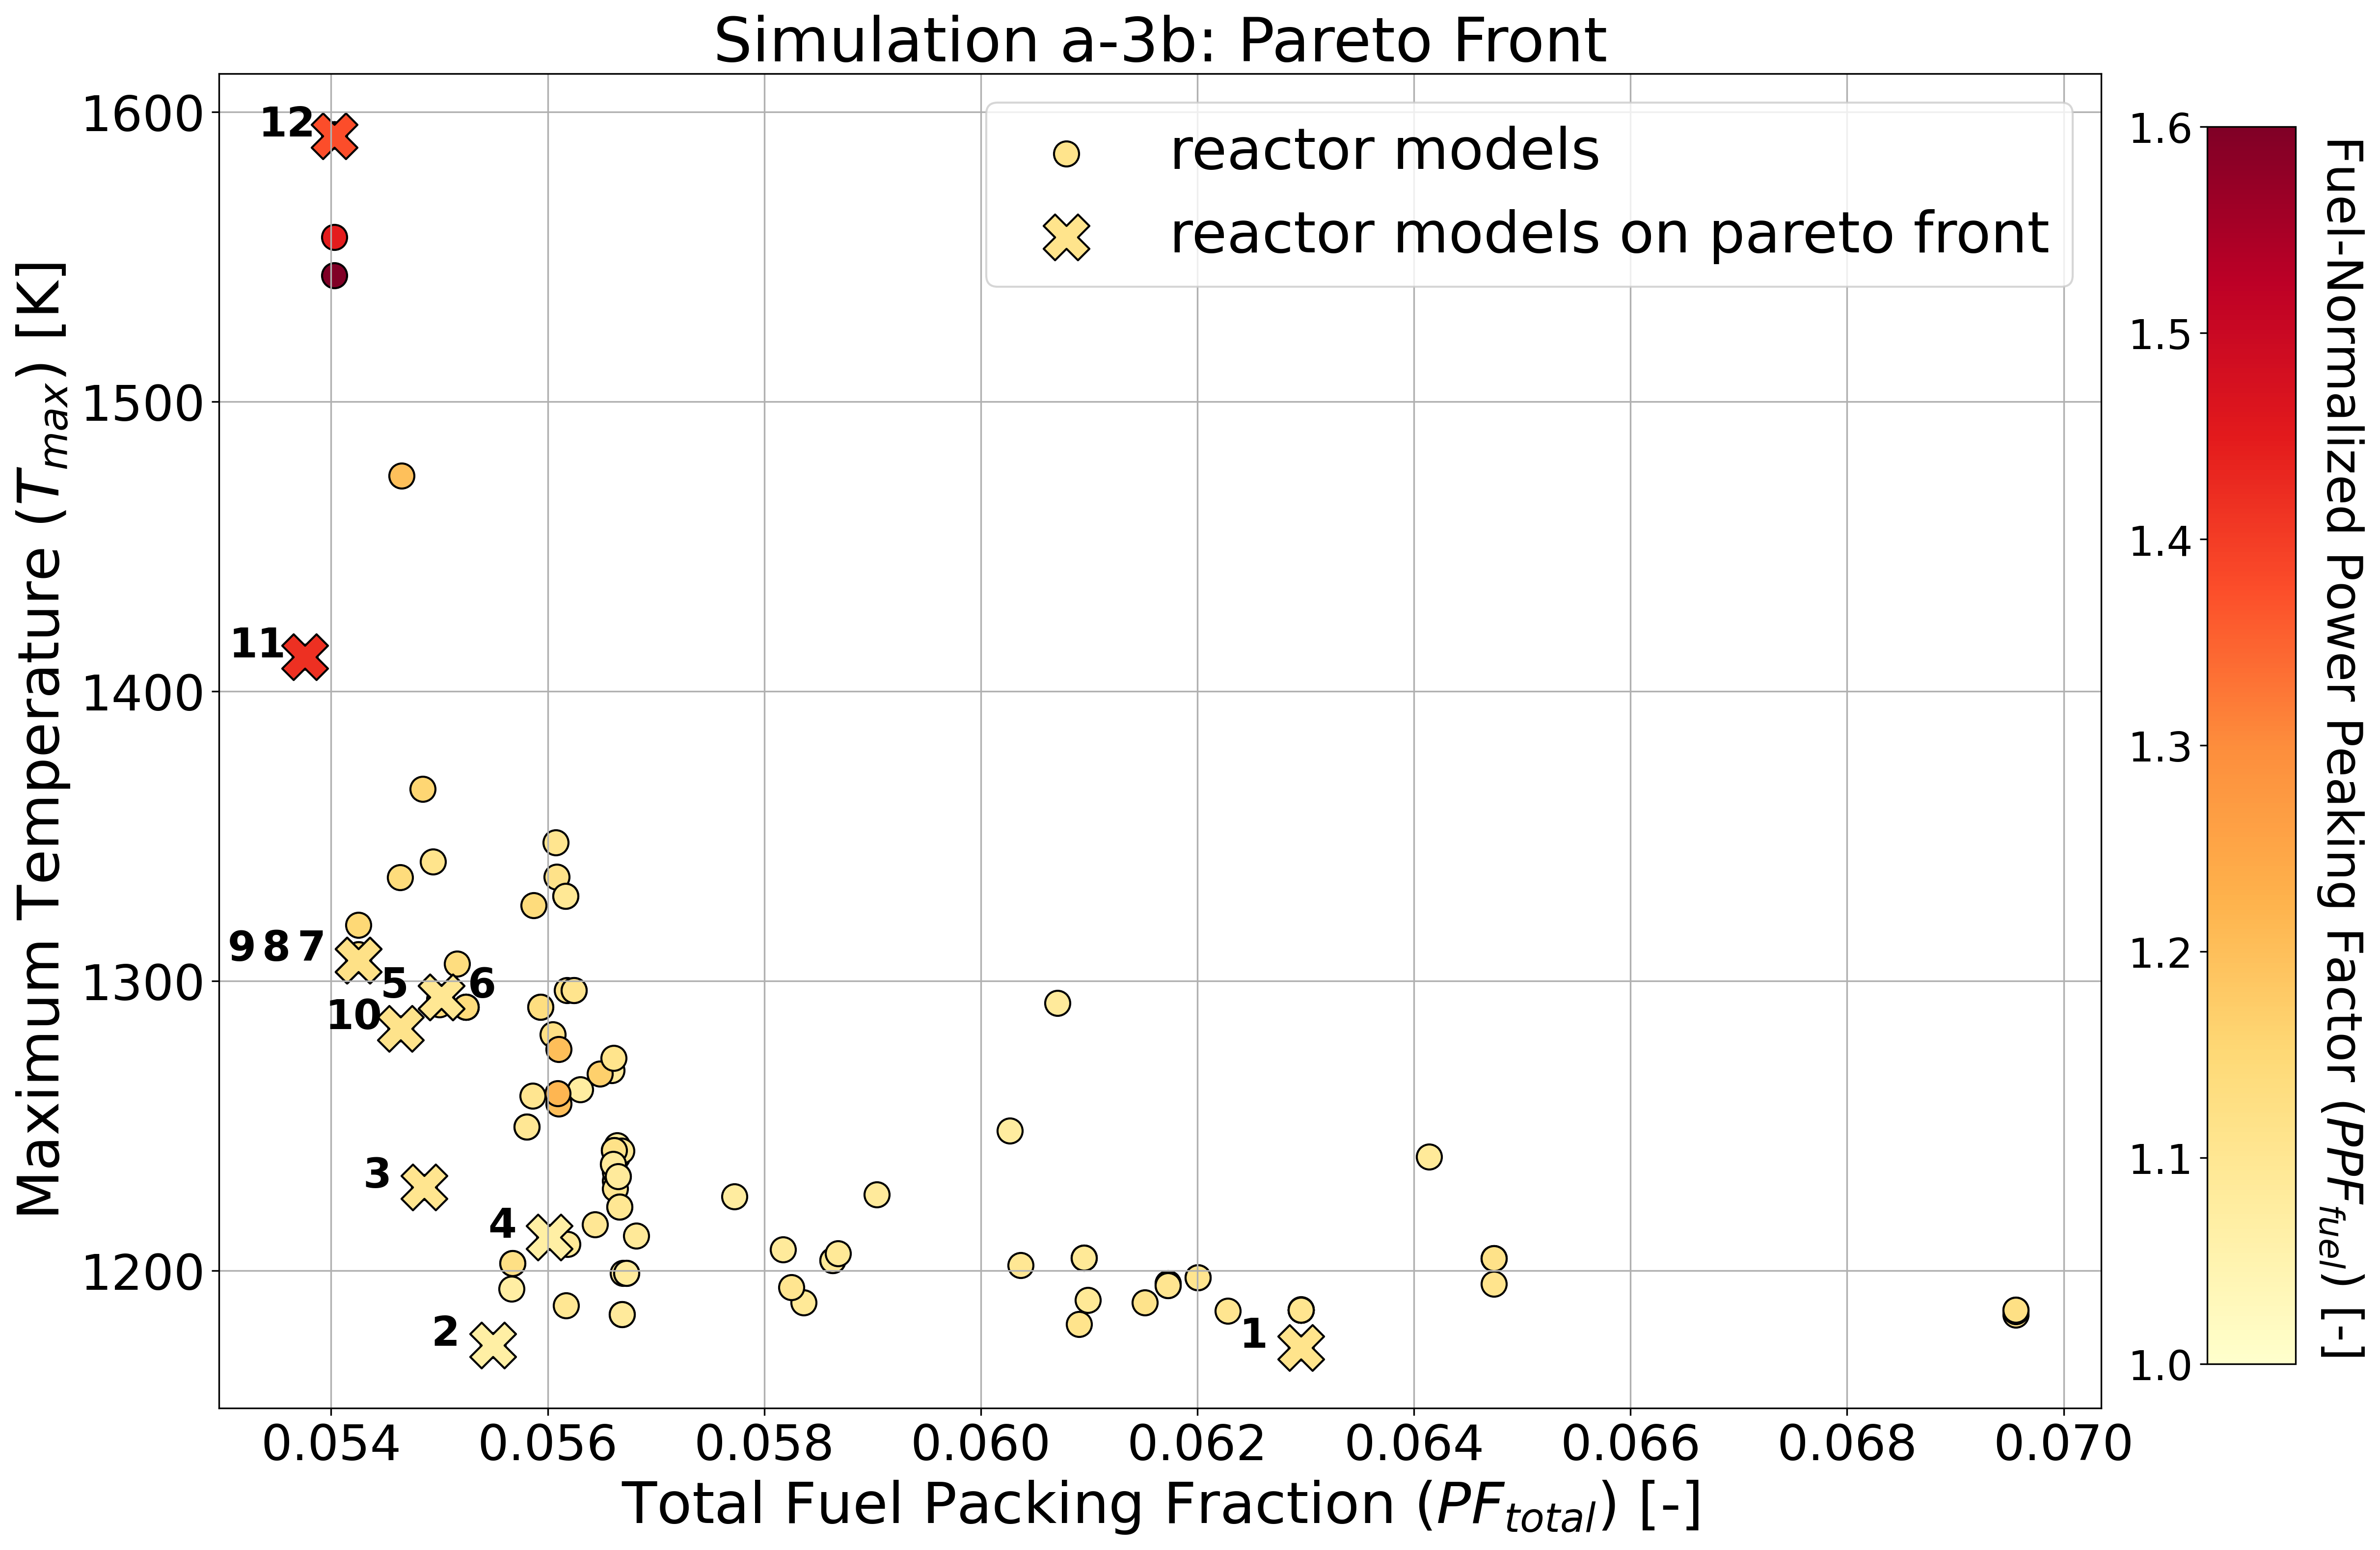
\includegraphics[width=\linewidth]{../docs/figures/assem-obj-3-all-2d.png} 
    \end{figure}
    \end{column}
\end{columns}
\end{frame}

\begin{frame}
    \frametitle{AHTR One-Third Assembly Simulation a-3b Results}
    \textbf{ROLLO found a wide variety of TRISO distr and coolant 
    channel shapes on the Pareto front that minimize each objective to different 
    extents.}

    \vspace{0.2cm}
    \begin{figure}
        \only<1>{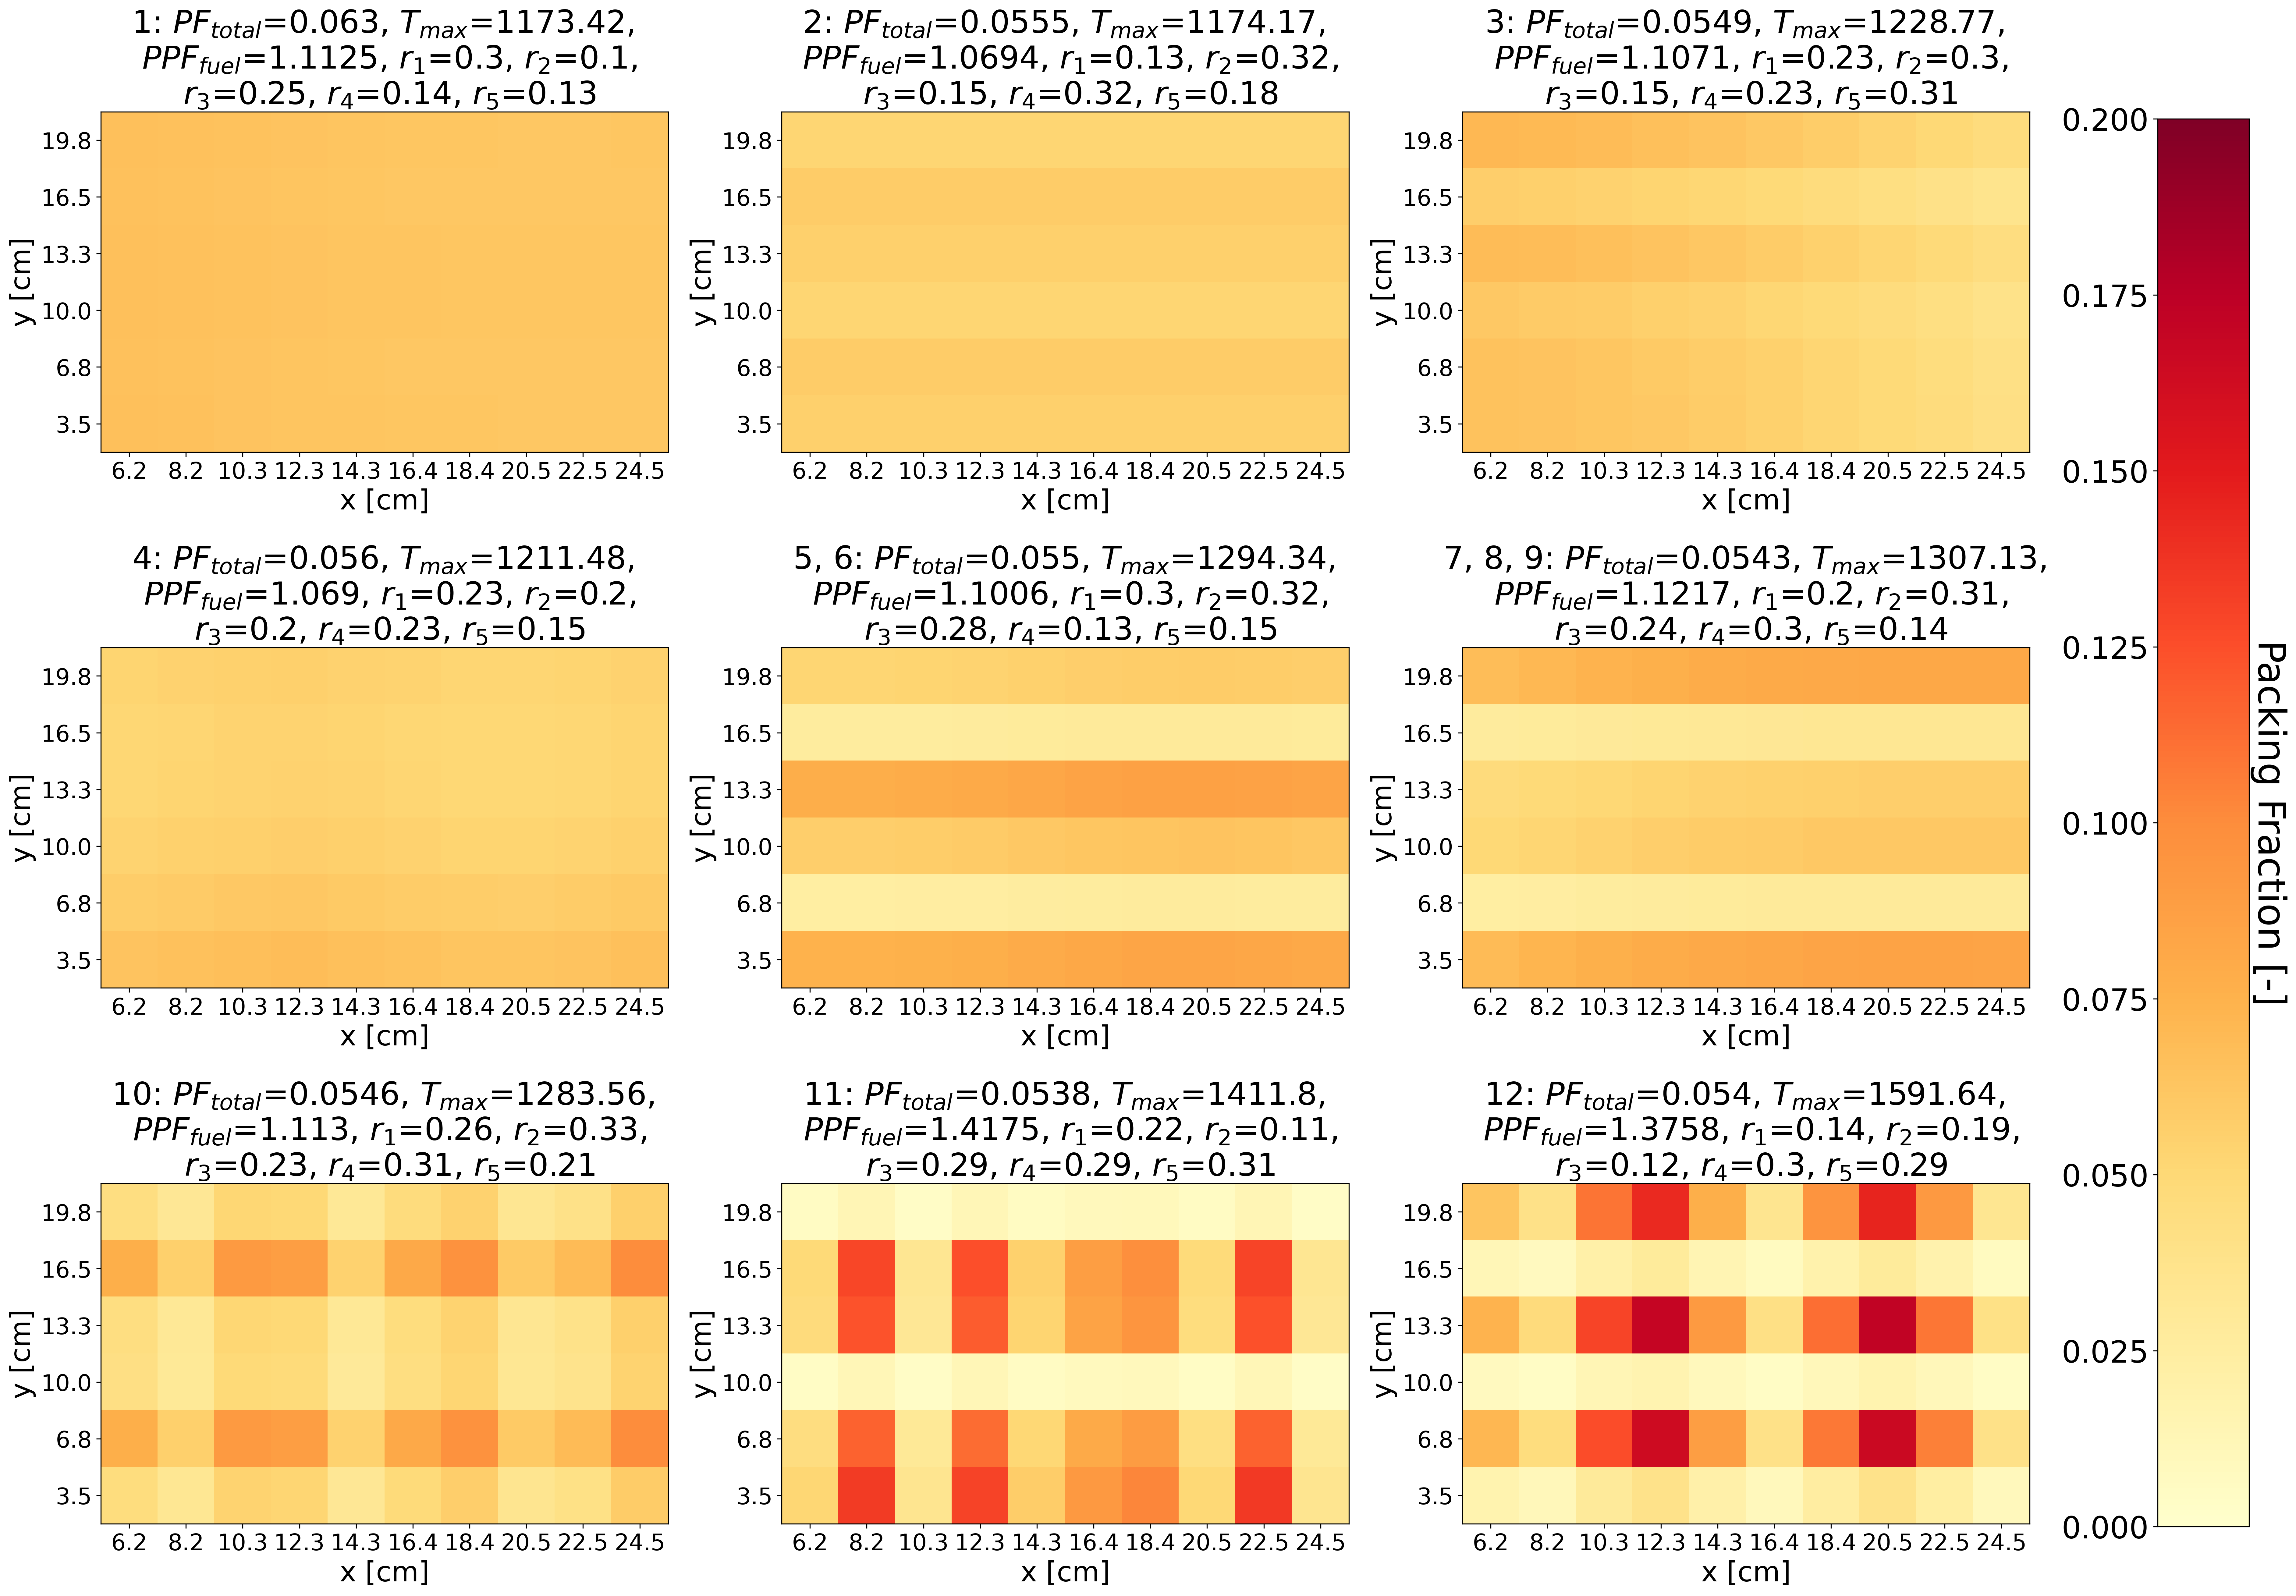
\includegraphics[width=0.7\linewidth]{../docs/figures/assem-obj-3-all-distr.png}}
        \only<2>{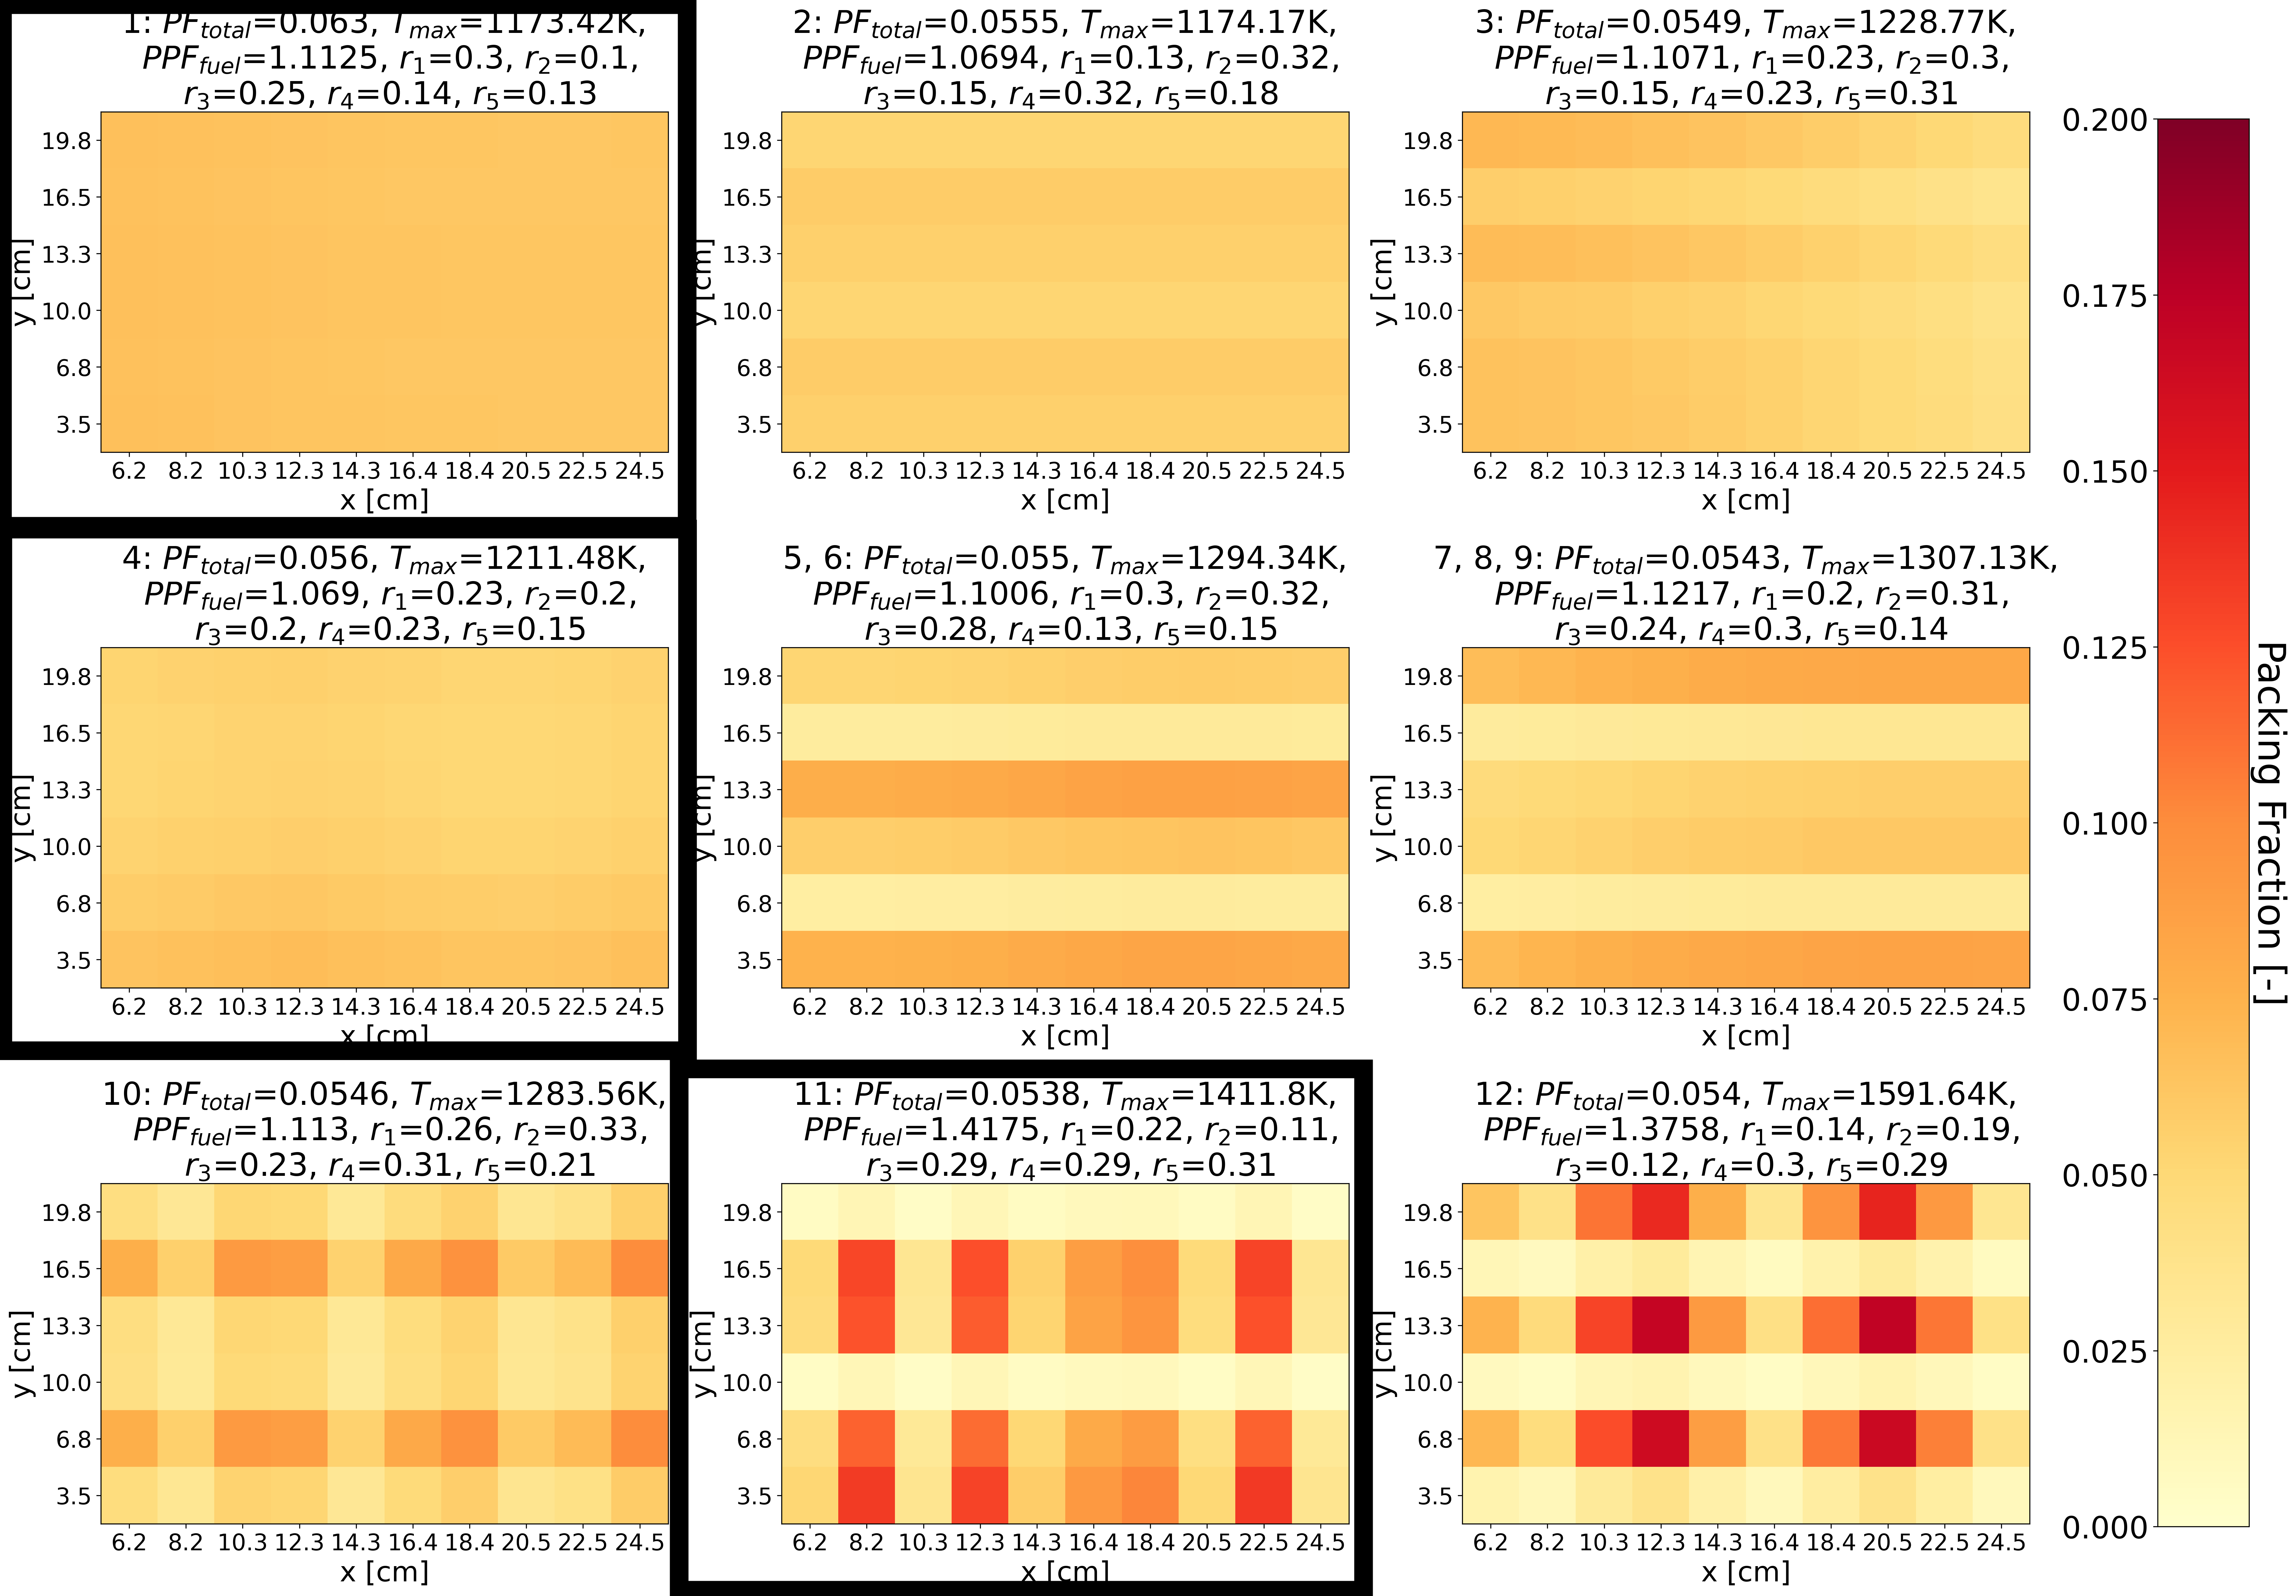
\includegraphics[width=0.7\linewidth]{figures/assem-obj-3-all-distr-annotated.png}}  
    \end{figure}
\end{frame}

\begin{frame}
    \frametitle{AHTR One-Third Assembly Simulation a-3b Results}
    \begin{columns}
        \begin{column}{0.6\textwidth}
        \begin{figure}
            \only<1,4>{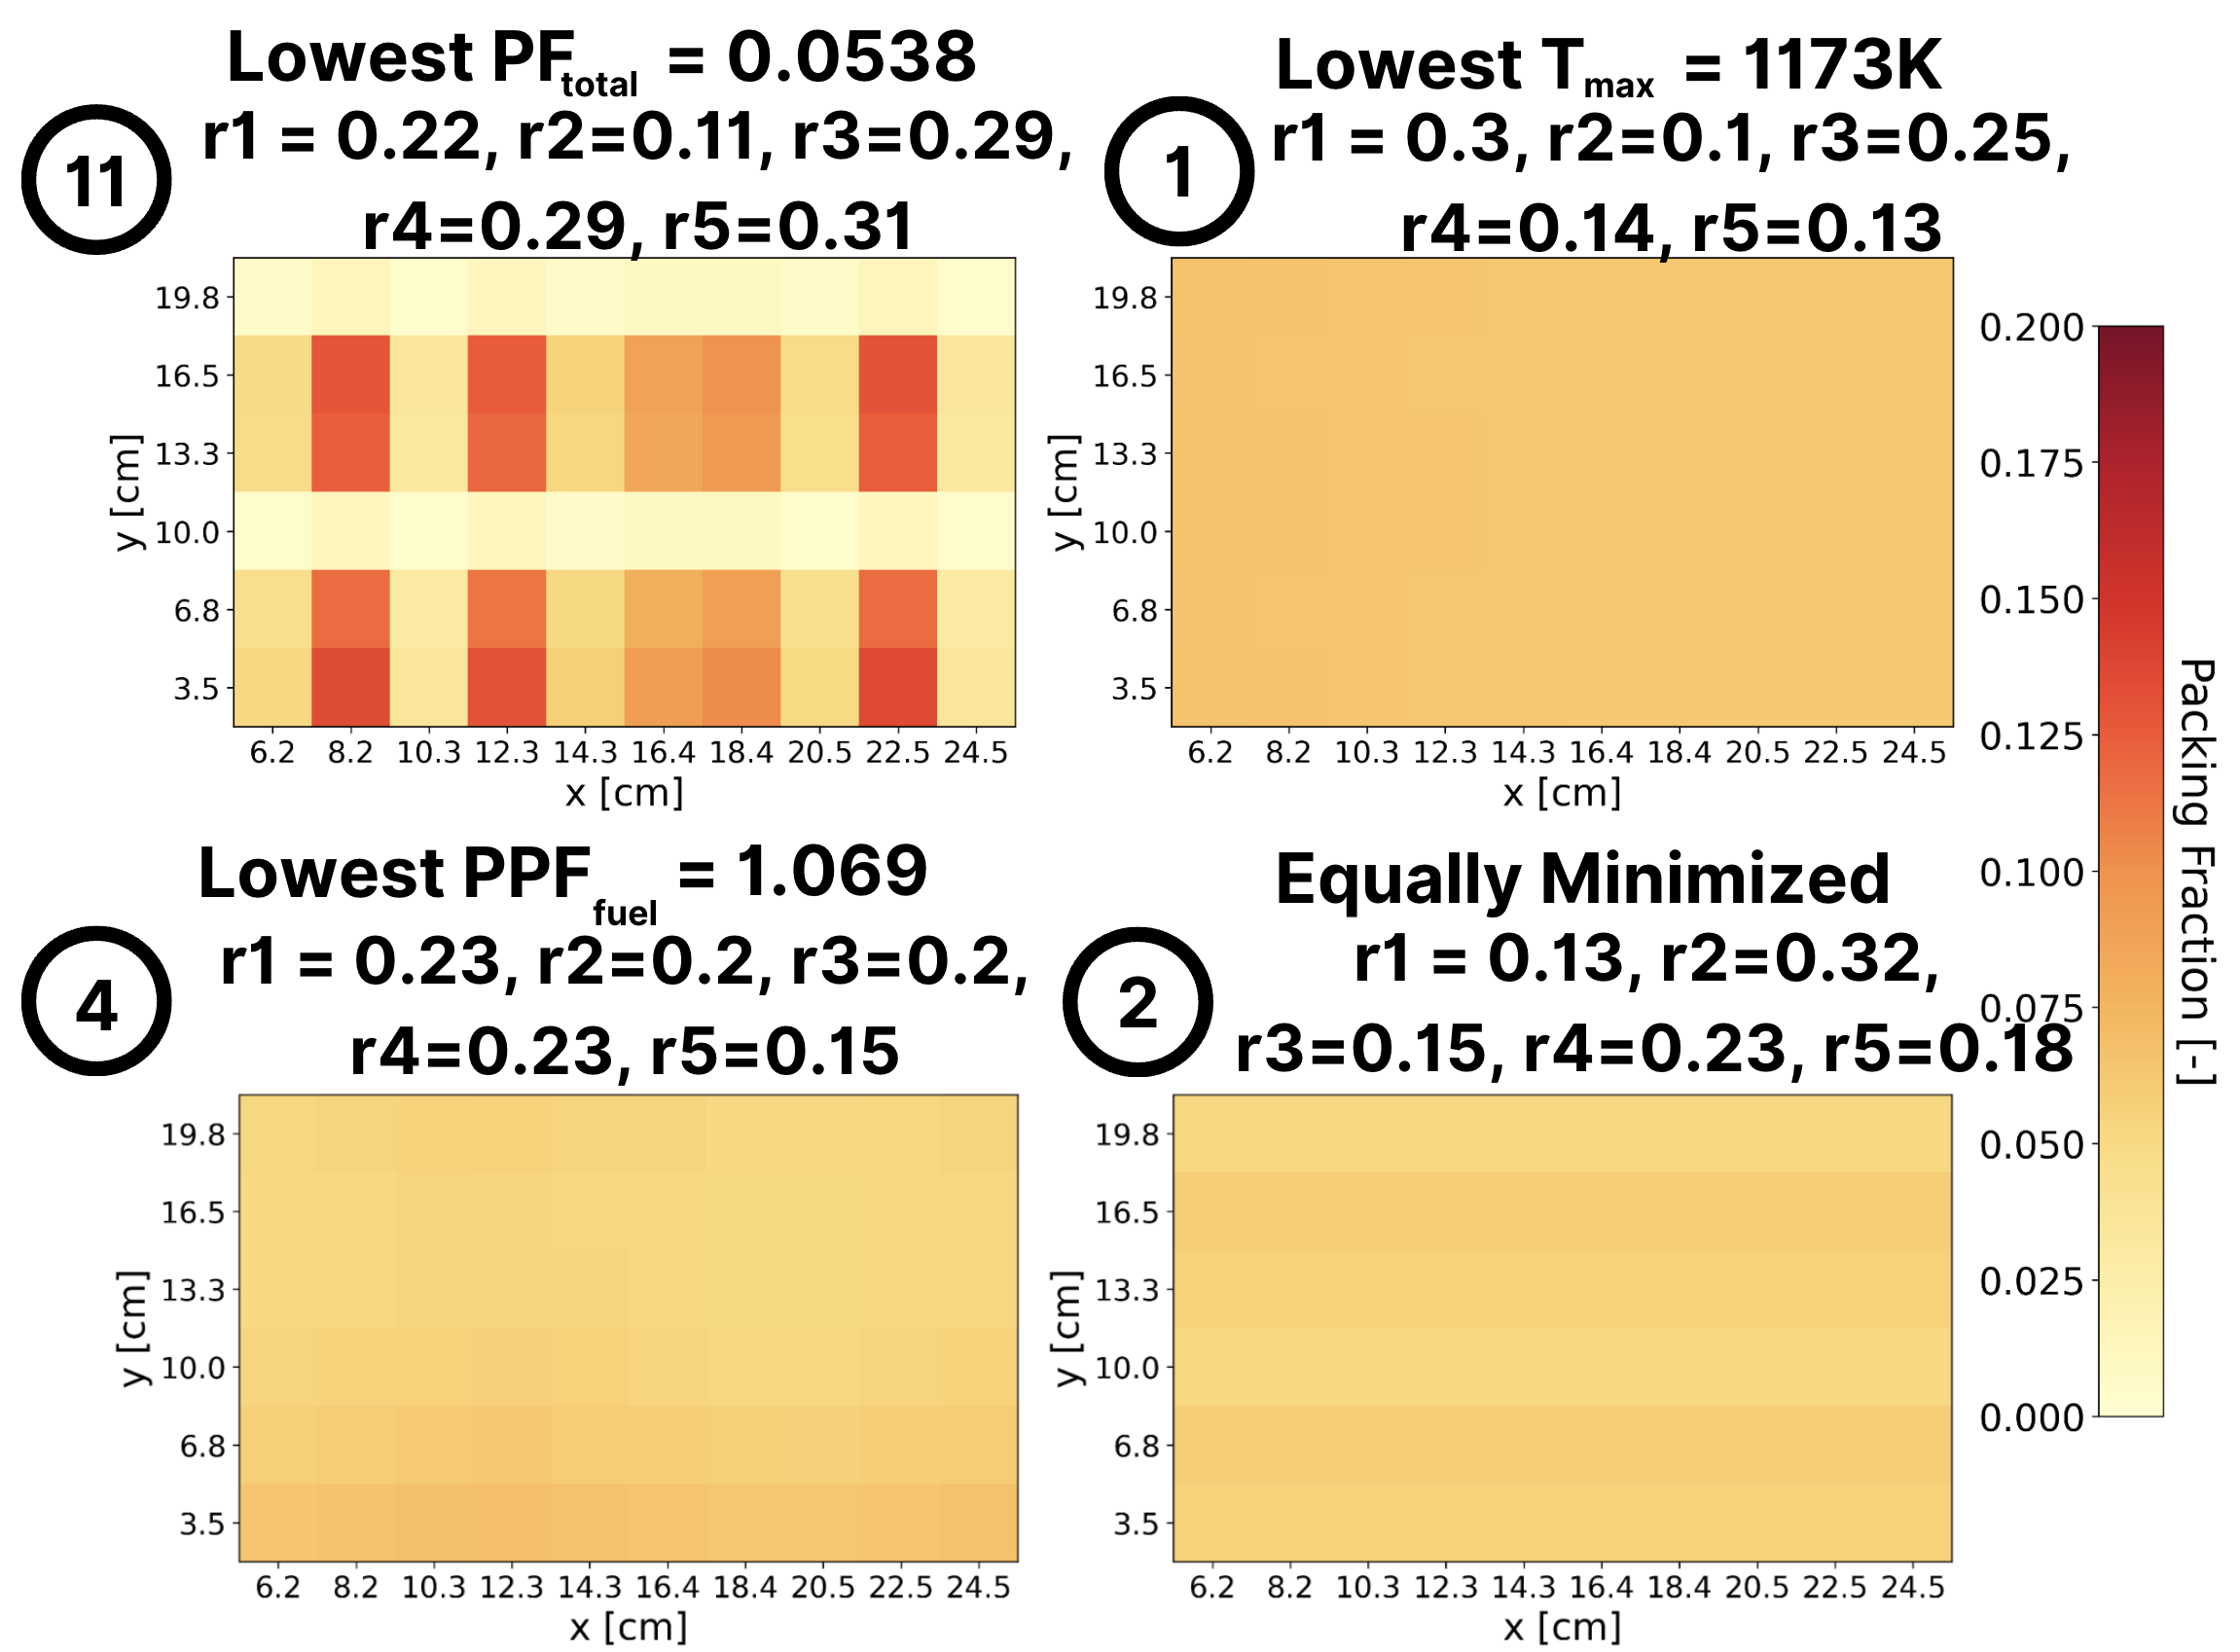
\includegraphics[width=\linewidth]{figures/a-3b-four-disr.png}} 
            \only<2>{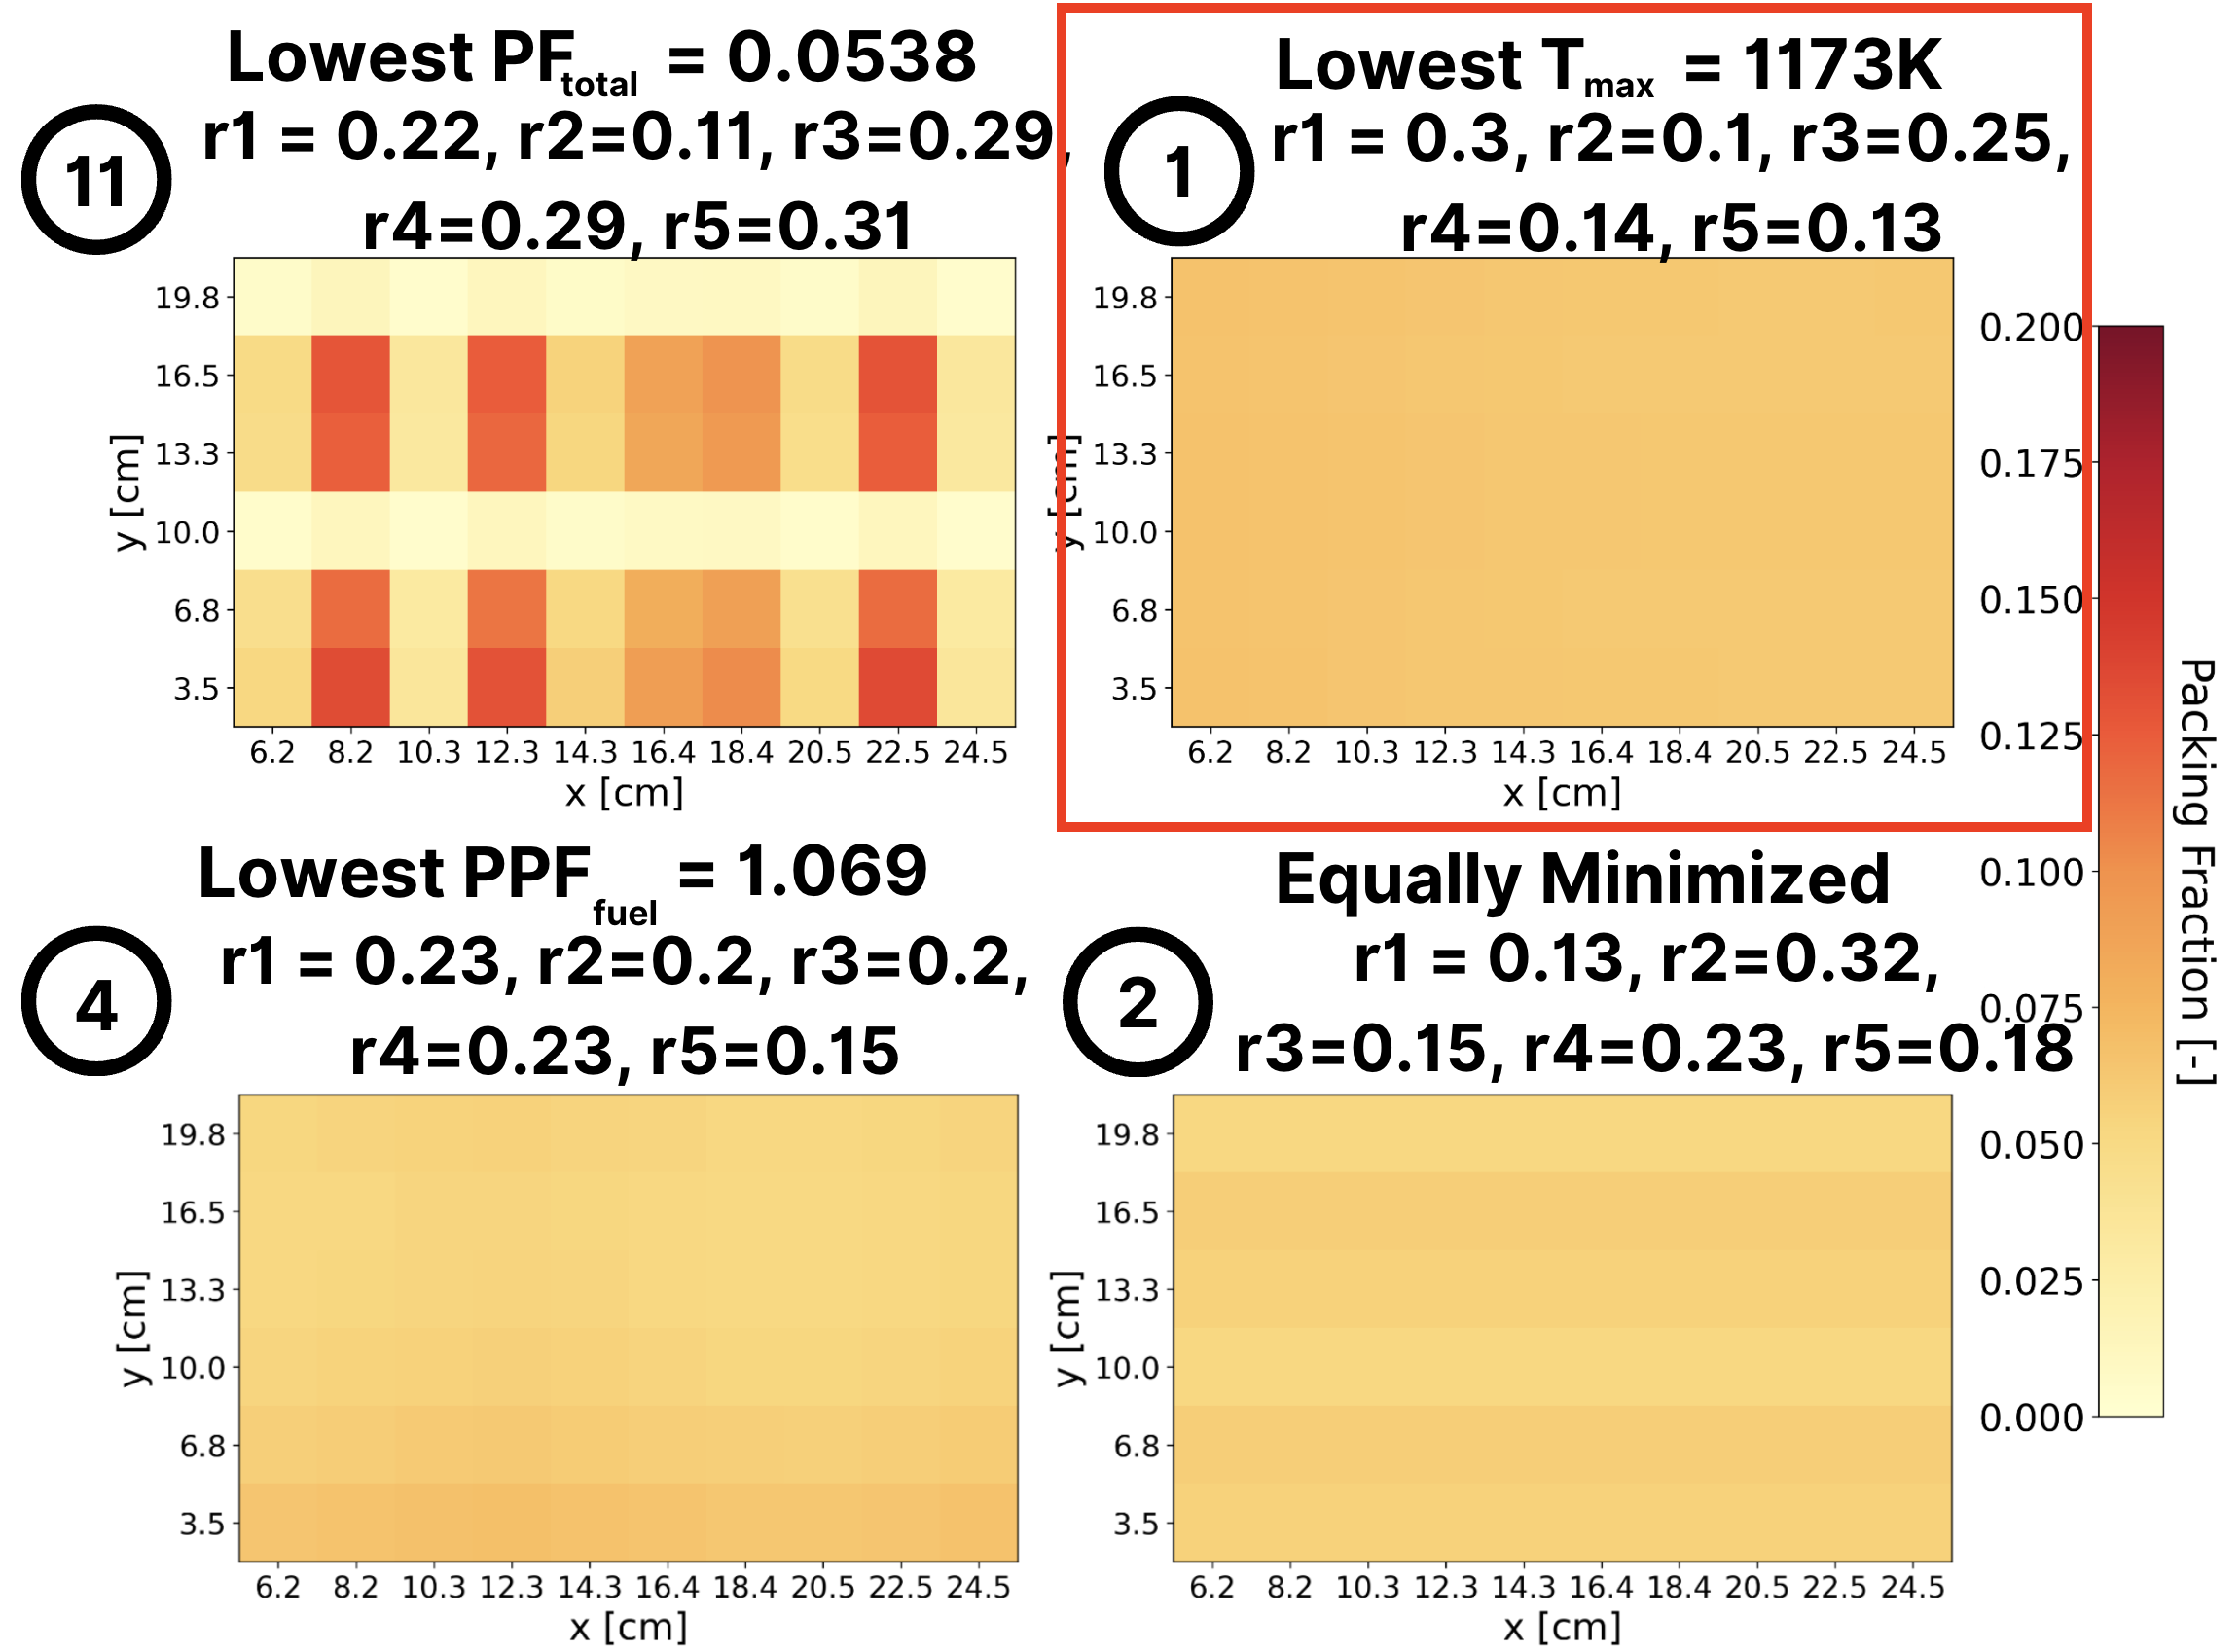
\includegraphics[width=\linewidth]{figures/a-3b-four-disr-annotated1.png}} 
            \only<3>{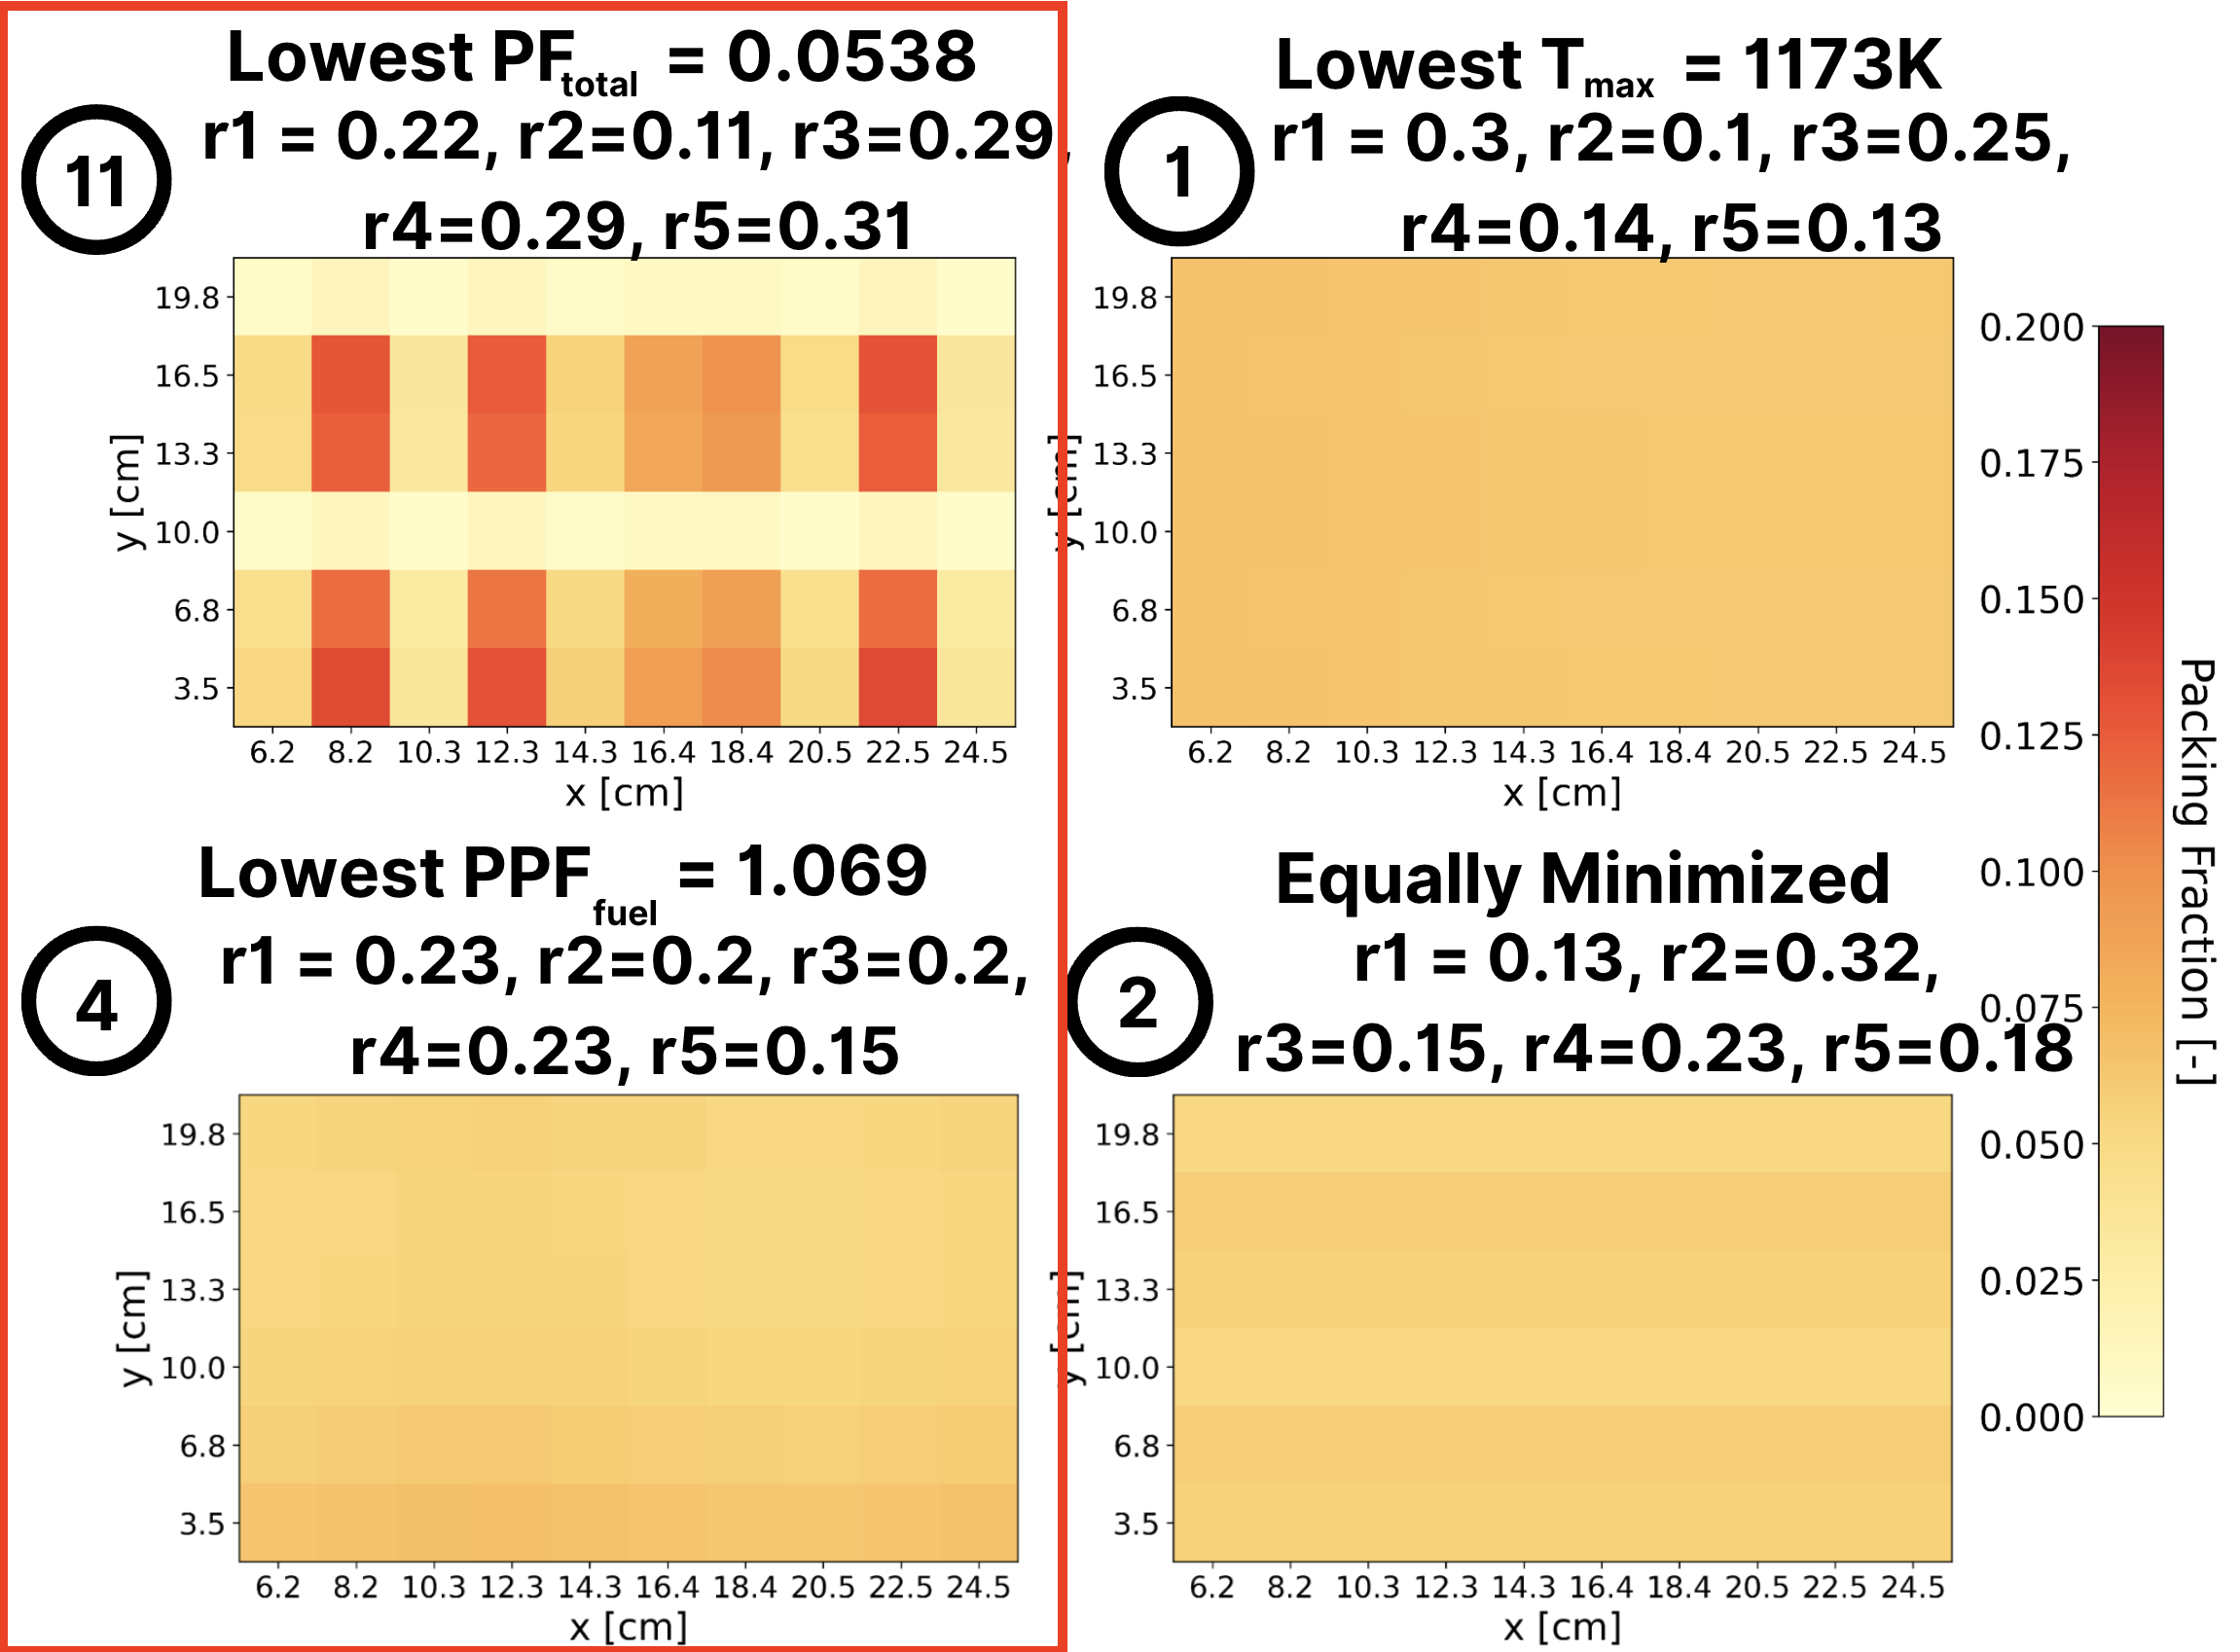
\includegraphics[width=\linewidth]{figures/a-3b-four-disr-annotated2.png}} 
        \end{figure}
        \end{column}
        \begin{column}{0.4\textwidth}
            \textbf{Key Observations}
            \begin{itemize}
                \visible<2->{\item TRISO distribution flatness is influenced by minimize $T_{max}$
                objective} 
                \visible<3->{\item Variations in TRISO distributions are influenced by minimize 
                $PF_{total}$ and $PPF_{fuel}$ objectives} 
                \visible<4->{\item Larger radius values are observed near temperature peaks} 
            \end{itemize}
        \end{column}
        \end{columns}
\end{frame}

\begin{frame}
    \frametitle{AHTR One-Third Assembly Simulation a-3b Results}
    \textbf{Simulation a-3b: One-third assembly model that equally minimized all 
    objectives (reactor model 2).}
    \begin{columns}
        \begin{column}{0.5\textwidth}
            \begin{figure}
                \only<1>{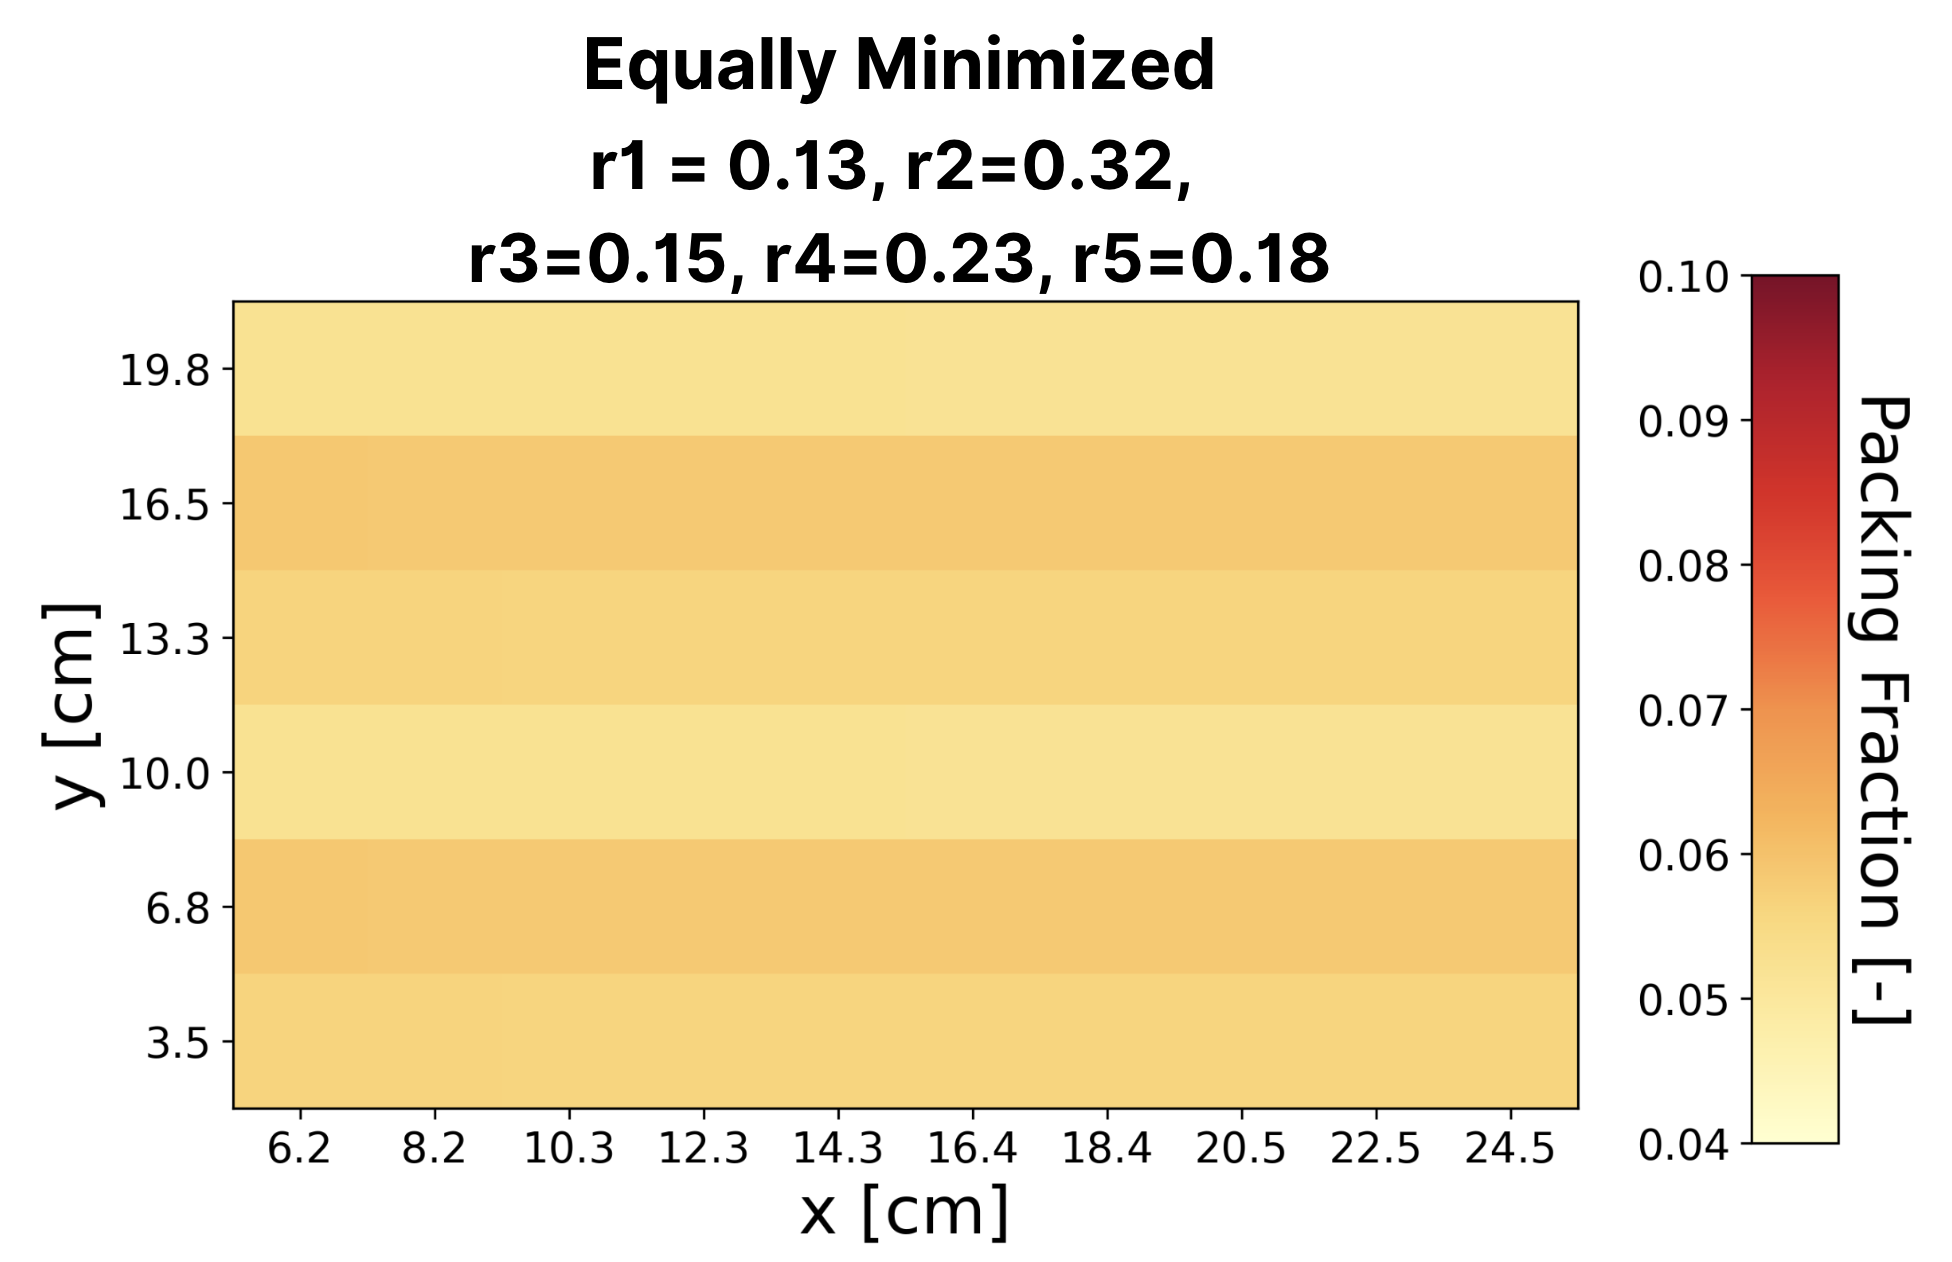
\includegraphics[width=\linewidth]{figures/a-3b-equal.png}}
                \only<2>{\makebox[\textwidth][c]{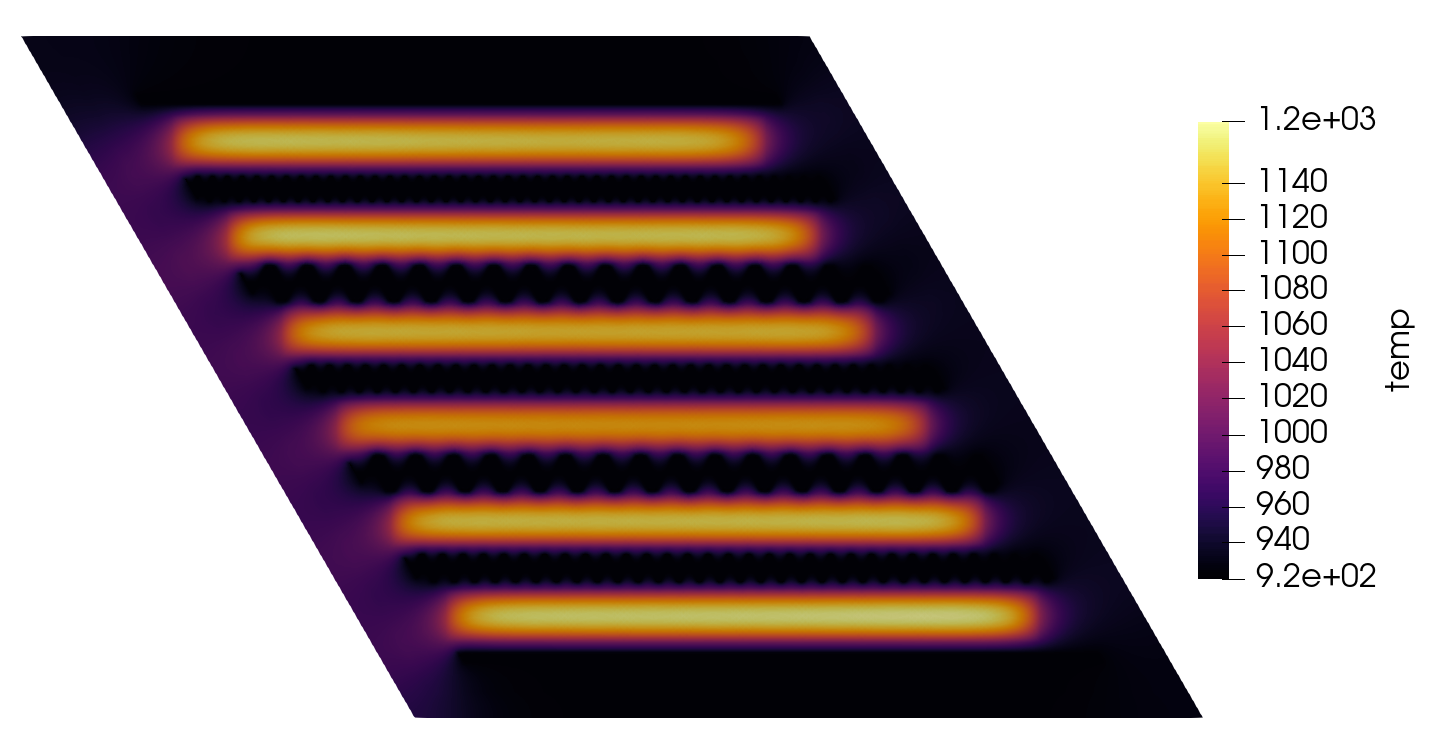
\includegraphics[width=1.1\linewidth]{figures/a-3b-temp.png}}}
            \end{figure}
        \end{column}
        \begin{column}{0.5\textwidth}
            \begin{figure}
                \makebox[\textwidth][c]{
                    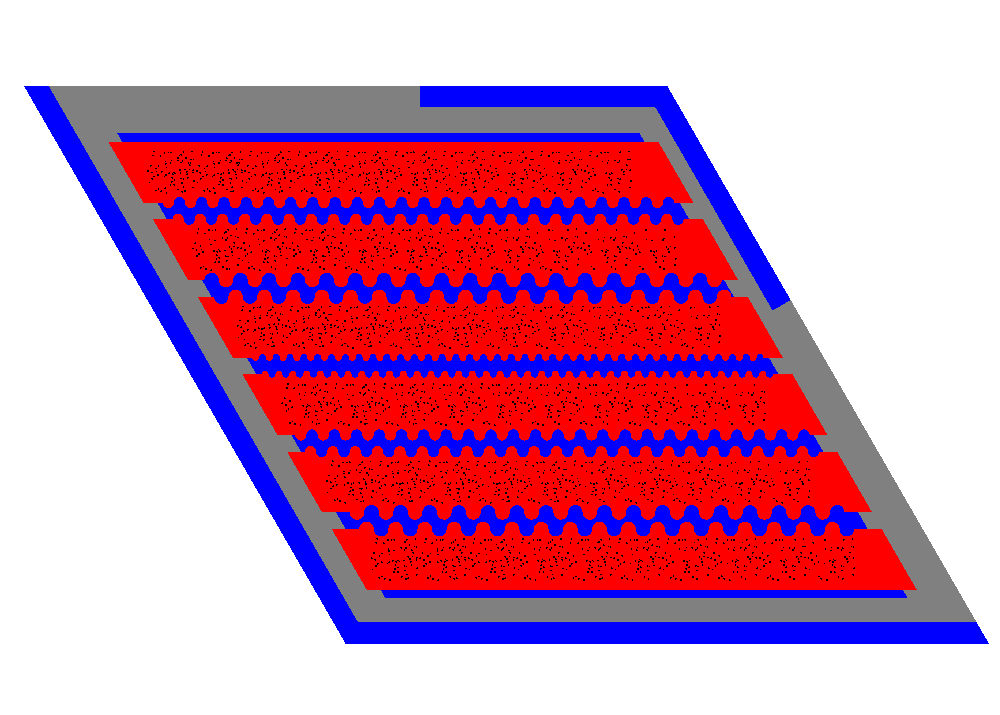
\includegraphics[width=1.1\linewidth]{../docs/figures/assem-obj-3-all-min-all.png}} 
            \end{figure}
        \end{column}
    \end{columns}
\end{frame}

\begin{frame}
    \frametitle{Multi-Objective Optimization Major Takeaways}
    \visible<1->{The multi-objective optimization simulations successfully explored the large 
    design space by finding \textbf{wide spread of reactor models on their 
    Pareto fronts}.} 

    \vspace{0.2cm}
    \visible<2->{The reactor models on the Pareto fronts have \textbf{different $PF_{total}$, 
    TRISO distributions, and coolant channel shapes}, depending on the extent 
    each objective is minimized due to the nature of multi-objective
    optimization that results in a \textbf{tradeoff between objectives}.} 

    \vspace{0.3cm}
    \visible<3->{\textbf{Minimize $T_{max}$ objective} 
    \begin{itemize}
        \item Continues to flatten TRISO distribution 
        \item Maximize radius values of FliBe channels located near temperature peaks
        \item TRISO distribution has a larger impact on $T_{max}$ than coolant channel 
        shape  
    \end{itemize}}

    \visible<4->{\textbf{Minimize $PF_{total}$ and $PPF_{fuel}$ objectives} 
    \begin{itemize}
    \item Influences variation in TRISO spatial distributions
    \item These two objectives influence each other to have unexpected TRISO
    distributions at different $PF_{total}$ values
    \end{itemize}}

\end{frame}

\begin{frame}
    \frametitle{ROLLO Tool + AHTR Optimization Simulations: Summary}
    \visible<1->{\begin{block}{I Successfully Completed AHTR Optimization for Non-conventional Designs
    Research Objectives}
    \begin{itemize}
        \item I developed \acrfull{ROLLO} tool that enables generative reactor design
        optimization with evolutionary algorithms 
        \item I demonstrated ROLLO's application on AHTR optimization for spatially variant 
        fuel distributions and wavy coolant channels
    \end{itemize}    
    \end{block}}
    \visible<2->{\begin{block}{Major Takeaways}
        \begin{itemize}
            \item Results demonstrate ROLLO's success in conducting a multi-objective 
            global search of the large AHTR design space to find optimal reactor models 
            that satisfy all the objectives
            \item Once the ROLLO search is complete, reactor designers gain a better 
            intuition of the model's reactor physics and can view the narrower reactor 
            design space that meets their defined objectives
        \end{itemize}
    \end{block}}
\end{frame}

\section{Conclusion}
\chapter{Conclusions and Future Work}
\glsresetall
\label{chap:concl}

Additive manufacturing of reactor core components removes the geometric constraints
required by conventional manufacturing, such as slabs as fuel planks, cylinders as 
fuel rods, etc, enabling further optimization and improvement of core geometries. 
Wide-spread adoption of additive manufacturing methods in the nuclear industry
could drastically reduce fabrication costs and deployment timelines, and improve 
reactor safety. 
Fully benefitting from the new ability to 3D print reactor components requires further 
research into reactor generative design optimization. 
This dissertation explores the new design space enabled by additive manufacturing 
by designing and applying the flexible and open-source \gls{ROLLO} tool to optimize 
the \gls{AHTR} for non-conventional geometries and parameters. 
I successfully explored the \gls{AHTR}'s arbitrary geometry design space by completing 
these three dissertation objectives: 
\begin{enumerate}
    \item I furthered our understanding of the \gls{AHTR} design's complexities 
    through neutronics and thermal-hydraulics modeling by participating in the 
    \gls{OECD} \gls{NEA} \gls{FHR} benchmark.
    \item I developed the open-source \gls{ROLLO} tool that enables generative reactor 
    design using evolutionary algorithm optimization for non-conventional reactor 
    geometries and fuel distributions.
    \item I applied \gls{ROLLO} to conduct generative \gls{AHTR} design.
    \gls{ROLLO} generated \gls{AHTR} designs with varying fuel amounts, fuel 
    distributions, and coolant channel shapes that optimize for three key reactor 
    performance metrics: minimize total fuel amount, maximize heat transfer, and 
    minimize power peaking.
\end{enumerate}
Chapter \ref{chap:fhr-benchmark} addressed objective 1, chapter \ref{chap:rollo} 
addressed objective 2, and chapters \ref{chap:method}, \ref{chap:ahtr-plank-opt-results}, 
and \ref{chap:ahtr-assem-opt-results} addressed objective 3. 

Chapter \ref{chap:fhr-benchmark} reported the \gls{FHR} benchmark Phase I-A and I-B 
results, highlighting the \gls{AHTR}'s passive safety behavior with 
negative temperature coefficients. 
Comparison of $k_{eff}$ results between the reference case and the \gls{AHTR} 
configuration with high heavy metal loading demonstrated that increased fuel 
packing does not always correspond with increased $k_{eff}$ due to self-shielding 
effects.
Chapter \ref{chap:fhr-benchmark} also reported the results of the \gls{AHTR} full 
assembly multiphysics model. The temperature distribution peaked in the fuel stripes near 
the spacers, highlighting to reactor designers that spacer material and location in the 
\gls{AHTR} geometry impact temperature peaks.  

Chapter \ref{chap:rollo} described the \gls{ROLLO} tool developed for this 
dissertation. 
\gls{ROLLO} is a Python package that applies evolutionary algorithm 
optimization techniques to generate nuclear reactor designs that meet user-defined 
objectives and constraints based on user-defined input value ranges. 
\gls{ROLLO} enables reactor designers to optimize any reactor model using robust 
evolutionary algorithm methods without going through the cumbersome process of setting up 
an evolutionary algorithm framework, selecting appropriate hyperparameters, and 
setting up parallelization.
\gls{ROLLO} is effective, flexible, open-source, parallel, reproducible, usable, and 
hosted on Github \cite{chee_rollo_2021}. 

% add more description to contextualize more so that the conclusion can stand on its own
Chapter \ref{chap:method} described the modeling and optimization methodology of the 
\gls{AHTR} plank and one-third assembly optimization conducted using the \gls{ROLLO} 
software.
I varied the following \gls{AHTR} plank and one-third assembly input parameters: 
\gls{TRISO} packing fraction distribution ($\rho_{TRISO}(\vec{r})$), total fuel 
packing fraction ($PF_{total}$), and coolant channel shape; in an effort to minimize 
the following objectives: total fuel packing fraction ($PF_{total}$), maximum 
temperature ($T_{max}$), and fuel-normalized power peaking factor ($PPF_{fuel}$). 

Chapter \ref{chap:ahtr-plank-opt-results} reported the \gls{AHTR} plank's 
\gls{ROLLO} optimization results.
I characterized each objective's driving factors and relationship 
with each input parameter from the results. 
I determined that the minimize $PF_{total}$ objective is driven by maximizing the plank's 
total fission reaction rate and influences oscillations in the TRISO distribution to 
achieve the objective. 
I determined that the minimize $PPF_{fuel}$ objective is driven by flattening the plank's
thermal flux distribution and influences $PF_{total}$ and oscillations in the TRISO 
distribution to achieve the objective.
I determined that the minimize $T_{max}$ objective flattens TRISO distribution and 
maximizes coolant channel shape's radius values to achieve the objective.
Characterizations of each objective for the simple \gls{AHTR} plank model provided 
insights for Chapter \ref{chap:ahtr-assem-opt-results}'s multi-objective 
optimization for the more complex \gls{AHTR} one-third assembly model. 

Chapter \ref{chap:ahtr-assem-opt-results} reported the \gls{AHTR} one-third assembly's
\gls{ROLLO} optimization results.
I verified that the one-third assembly objectives follows the same driving 
factors as the \gls{AHTR} plank optimization objectives. 
The results demonstrated that the minimize $PF_{total}$ objective's driving factor 
maximize total fission reaction rate and minimize $PPF_{fuel}$ objective's driving 
factor flattening thermal flux distribution influenced each other resulting in unexpected 
TRISO distributions at different $PF_{total}$ values. 
Further optimization of the \gls{AHTR} design will benefit from awareness 
of the objectives' relationship. 
The results also demonstrated that the coolant channel shape variation did 
not have as high of an impact on $T_{max}$ as \gls{TRISO} distribution variation.
Simulation a-3b-256's multi-objective optimization showed the result of minimizing all 
three objectives ($PF_{total}$, $T_{max}$, and $PPF_{fuel}$) while varying 
all the input parameters ($PF_{total}$, TRISO distribution, and coolant channel shape).
Figure \ref{fig:assem-obj-3-all-256} showed the 38 reactor models on simulation 
a-3b-256's Pareto front that met all three objectives. 
The reactor models on the Pareto Front have different $PF_{total}$, TRISO distributions, 
and coolant channel shapes, depending on the extent each objective is minimized due 
to the nature of multi-objective optimization that results in a tradeoff between 
objectives. 
These results demonstrate that the generative design optimization process with \gls{ROLLO}
provides the reactor designer with a set of equally good reactor models. 
From this point, it is up to the reactor designer to determine the importance of each 
objective for their purposes, then conduct further sensitivity analysis and 
use higher fidelity models to study the optimal design space before selecting 
the final reactor model.

Chapters \ref{chap:ahtr-plank-opt-results} and \ref{chap:ahtr-assem-opt-results} 
demonstrated \gls{ROLLO}'s success in conducting multi-objective generative reactor 
design optimization. 
\gls{ROLLO} conducted a global search of the large reactor design space and successfully 
generated optimal reactor models on the Pareto front that satisfy all the objectives. 
\gls{ROLLO} also showed how sensitive each input parameter is in relation to 
the objectives. 
Once the \gls{ROLLO} search is complete, reactor designers gain a better intuition of 
the model's reactor physics and can view the narrower reactor design space that meets 
their defined objectives.   

\section{Future Work}
This dissertation's generative design optimization of the \gls{AHTR} model used sine 
distribution variations to govern the \gls{TRISO} packing fraction distribution and  
varied cylinder radius' to generate varying sinusoidal-like pattern coolant channel 
shapes. 
These input parameter variations are only one way to represent the \gls{AHTR} 
geometry. 
There are many other ways to represent the geometry that might give \gls{ROLLO} more 
freedom to explore a larger design space and generate more optimized designs. 
Future reactor designers could consider topology optimization to optimize coolant 
channel shape further.
The major limitation is the computational cost of modeling fluid flow in complex 
coolant channel designs. 

This dissertation demonstrated \gls{ROLLO}'s success in conducting multi-objective 
generative reactor design optimization. 
\gls{ROLLO} can be easily used to optimize any reactor type for any perceivable 
arbitrary input parameters. 
As additive manufacturing technology advances and the \gls{TCR} program 
demonstrates the first 3D printed operational reactor, more reactor designers 
will begin to explore the vast design space enabled by 3D printing. 
Future work includes utilizing \gls{ROLLO} to optimize other reactor types. 
By designing the \gls{ROLLO} tool and demonstrating its success in further optimization 
of the \gls{AHTR} beyond classical input parameters, this dissertation contributes to 
improving reactor technology to ensure that nuclear energy continues to provide 
low-carbon electricity worldwide.


%\input{acks}
%%--------------------------------%%
%%--------------------------------%%
\begin{frame}[allowframebreaks]
  \frametitle{References}
  \bibliographystyle{ieeetr}
  {\footnotesize \bibliography{../docs/2022-chee-dissertation.bib} }

\end{frame}

%\section*{Appendix}
%\subsection*{Grad School Journey}
\begin{frame}
    \frametitle{Grad School Journey}
    \vspace{-0.2cm}
    \begin{figure}[]
        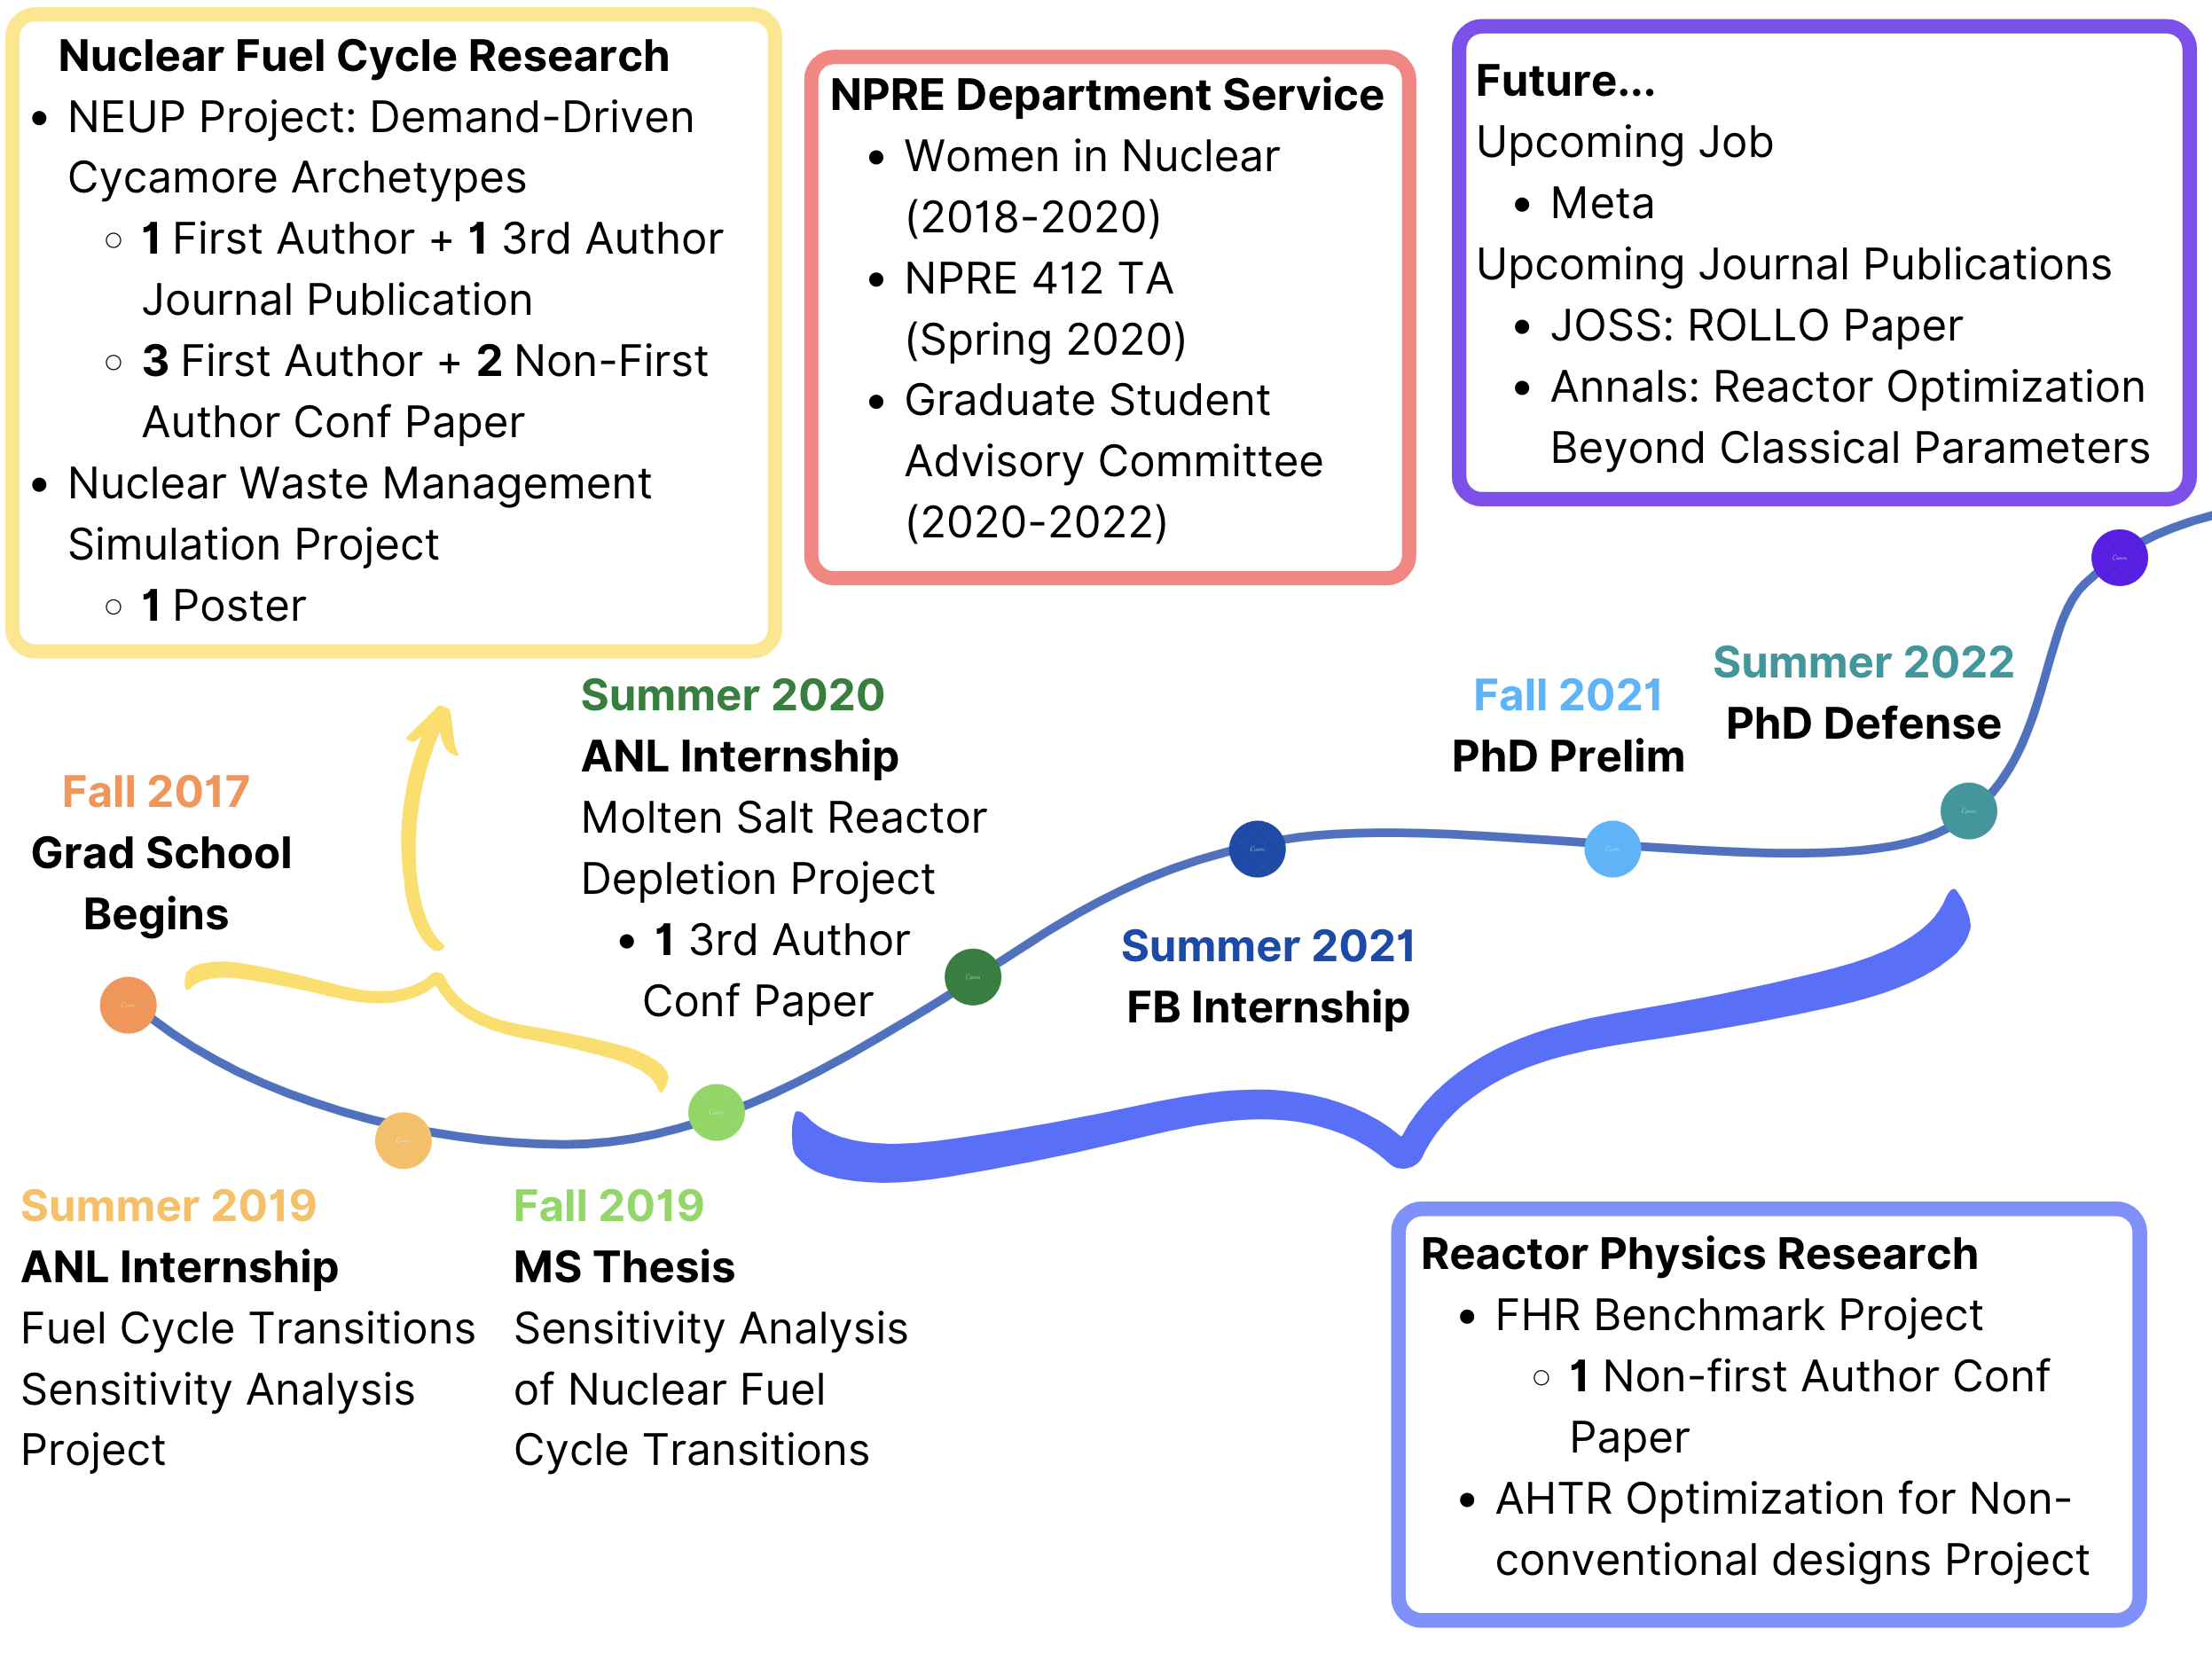
\includegraphics[width=0.9\linewidth]{figures/grad-school-journey.png} 
    \end{figure}
\end{frame}

\subsection*{Summary}
\begin{frame}
    \frametitle{Summary}
    \begin{columns}[t]
        \begin{column}{0.5\linewidth}
            \begin{block}{AHTR Model Development for the FHR Benchmark}
                \textbf{Results Presented} 
                \begin{itemize}
                    \item FHR benchmark Phase I-A and I-B results
                    \item AHTR full assembly temperature model 
                \end{itemize}

                Through participation in the FHR benchmark, this dissertation contributes to 
                \textbf{deepening our understanding of the promising \gls{AHTR} technology}.
            \end{block}
        \end{column}
        \begin{column}{0.5\linewidth}
            \begin{block}{ROLLO Tool Development and AHTR Non-Conventional Design Optimization}
                \textbf{Results Presented}
                \begin{itemize}
                    \item \acrfull{ROLLO} tool 
                    \item AHTR Optimization for heterogeneous fuel distributions and wavy 
                    coolant channels 
                \end{itemize}
                
                By designing the ROLLO tool and demonstrating its success in 
                optimization of the \gls{AHTR} beyond classical input parameters, this dissertation 
                contributes to \textbf{optimization tool development for reactors of the future}.
            \end{block}
        \end{column}
    \end{columns}
\end{frame}

\subsection*{FHR Benchmark Specifications}
\begin{frame}
    \frametitle{FHR Benchmark Specifications}
    UIUC participates in the benchmark with OpenMC and using the ENDF/B-VII.1 material 
    cross section library
    \vspace{-0.2cm}
    \begin{table}
        \caption{OECD NEA's FHR Benchmark Phases 
        \cite{petrovic_benchmark_2021}.}
        \vspace{-0.25cm}
        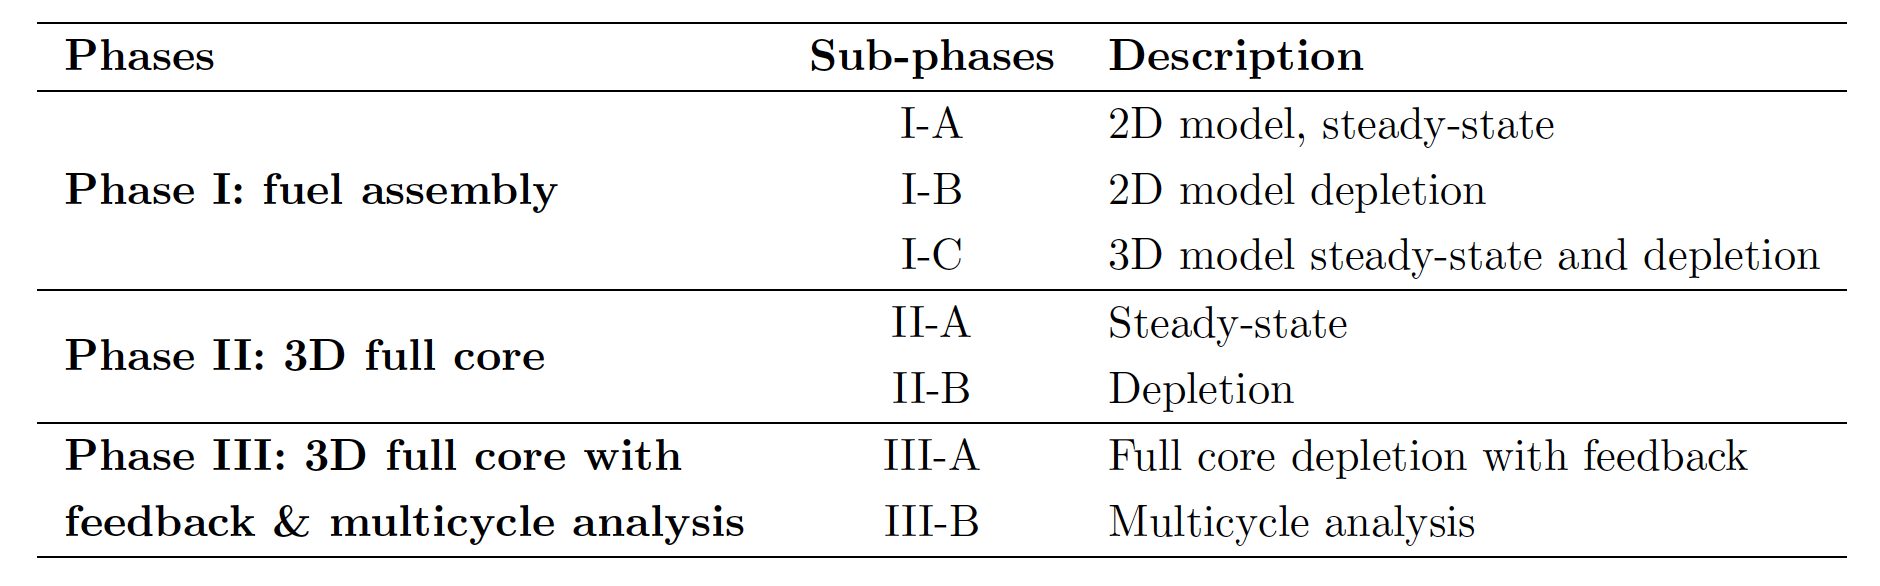
\includegraphics[width=0.7\linewidth]{figures/benchmark-phases.png} 
    \end{table}
    \vspace{-0.3cm}
    \begin{figure}[]
        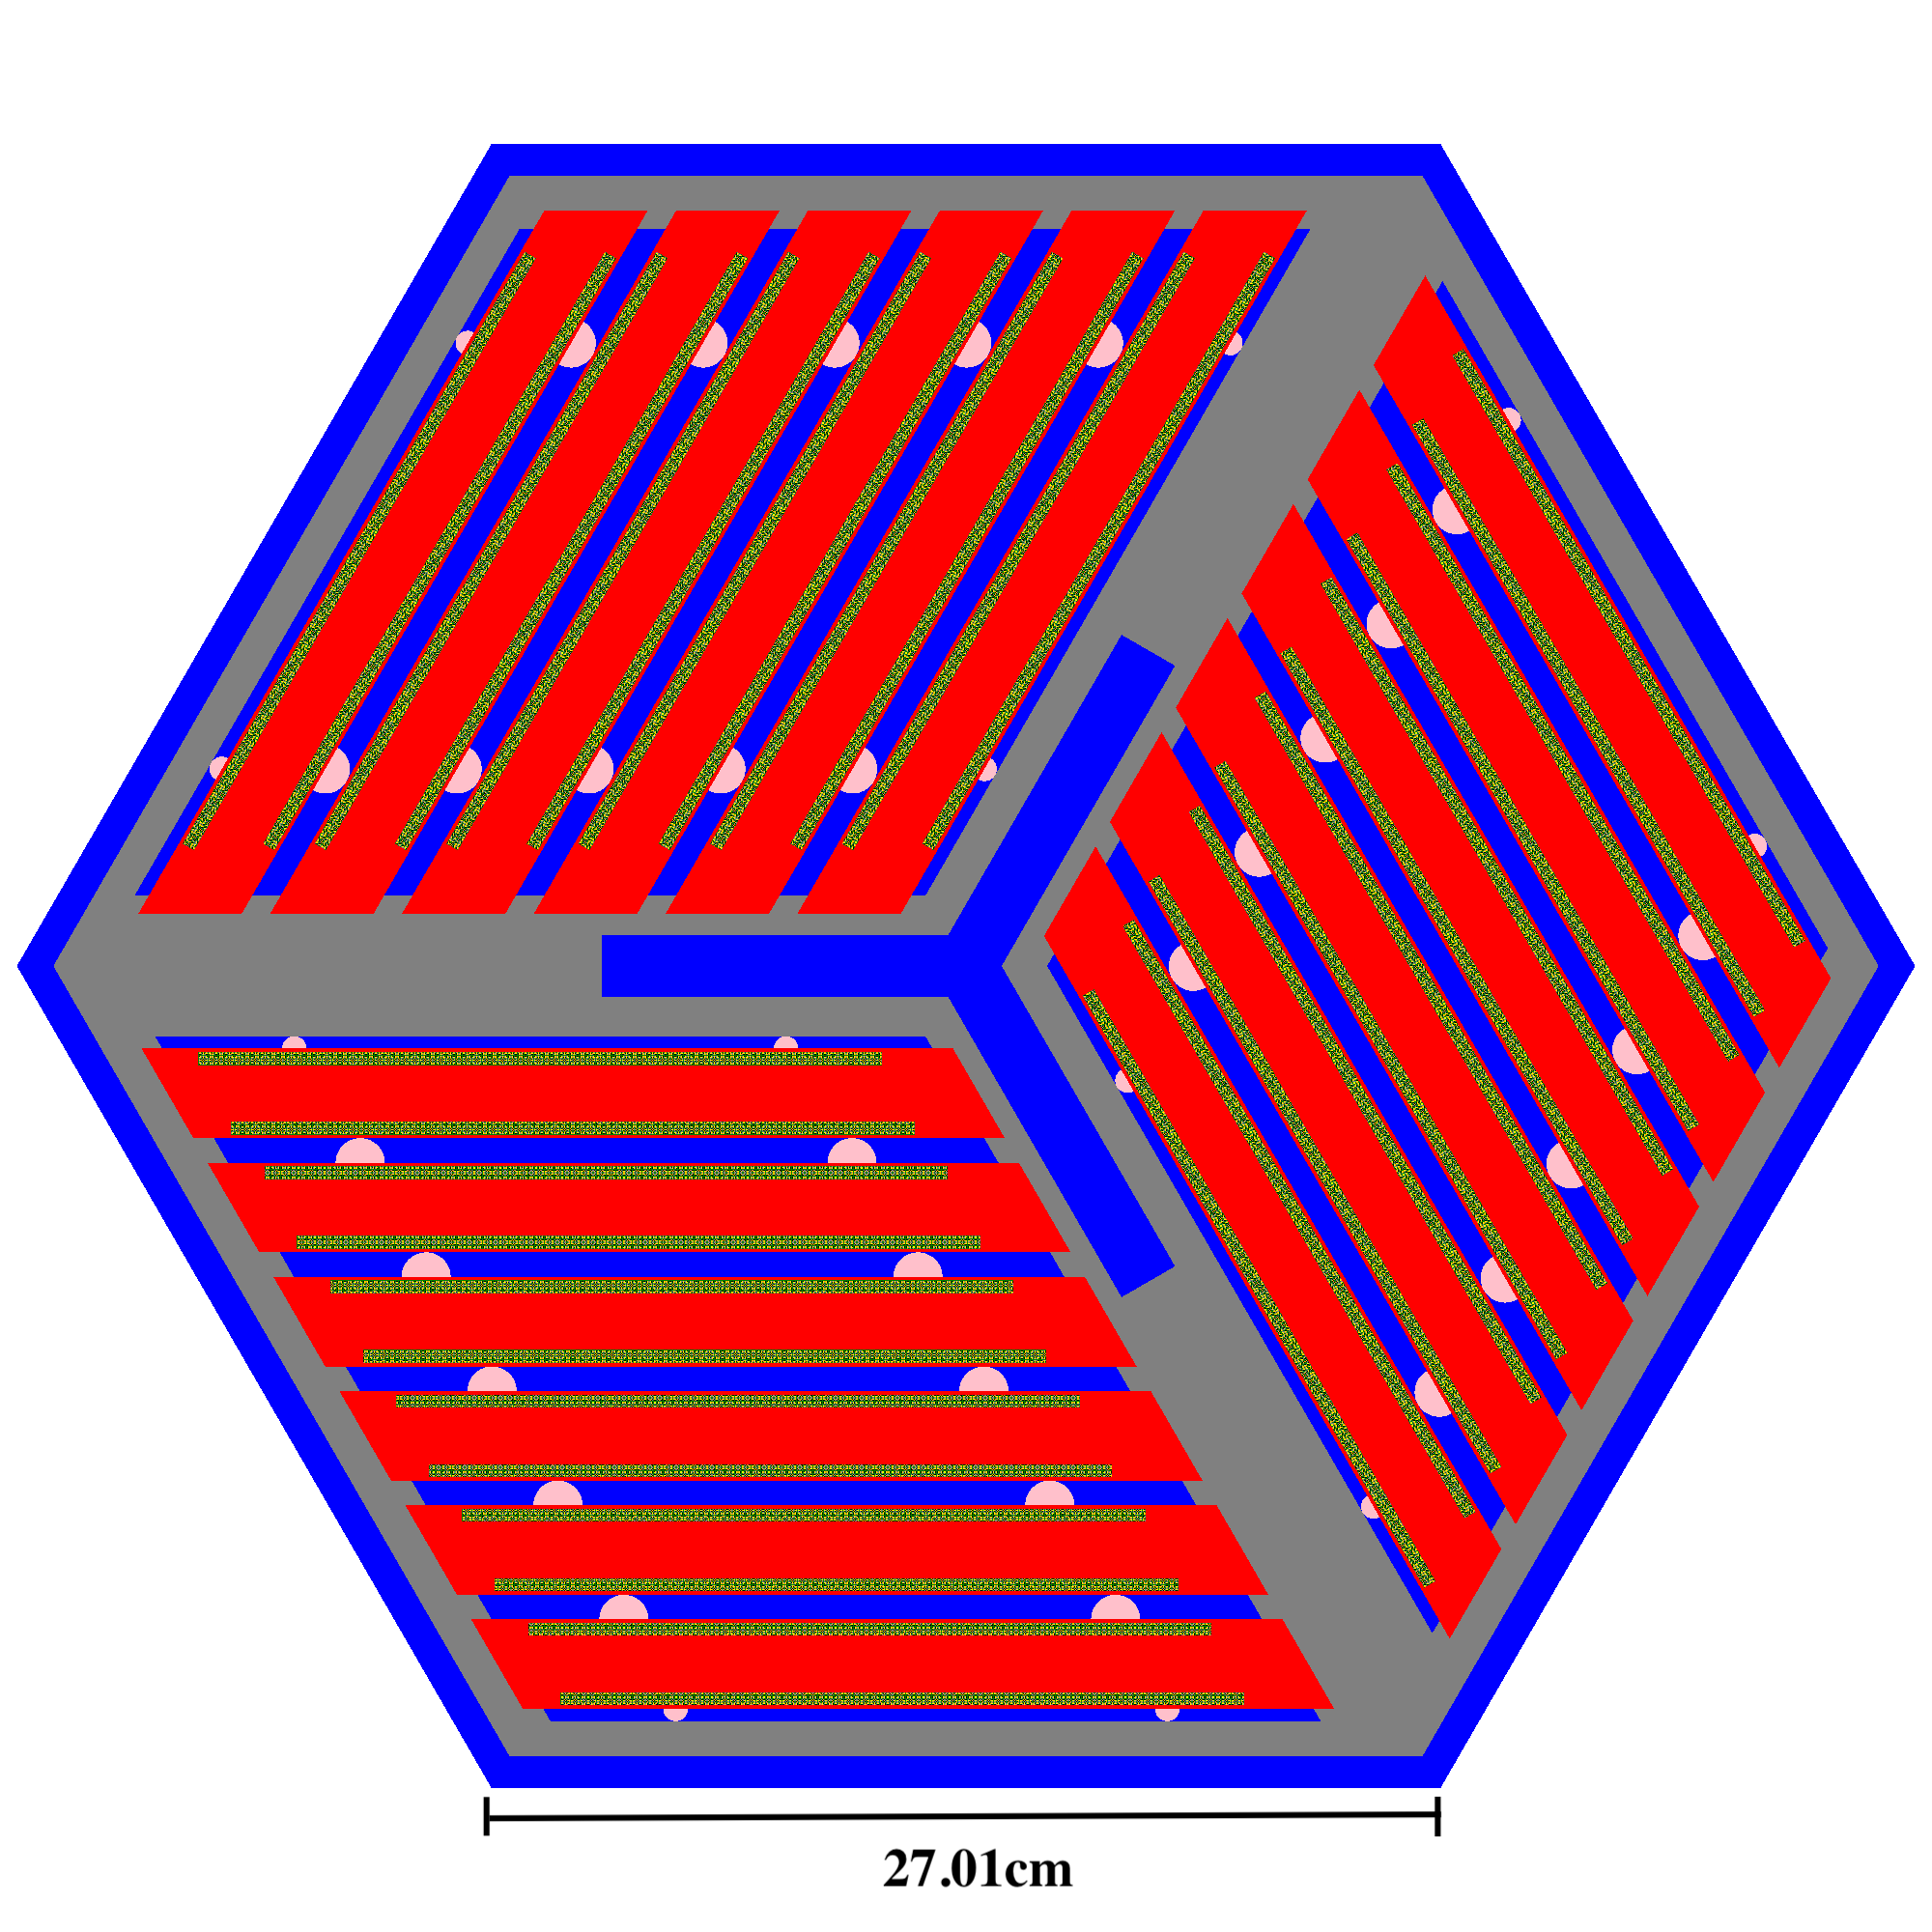
\includegraphics[width=0.27\linewidth]{../docs/figures/ahtr-fuel-element.png} 
        \vspace{-0.2cm}
        \caption{AHTR fuel assembly.}
    \end{figure}
\end{frame}

\begin{frame}
    \frametitle{FHR Benchmark Specifications}
    Only Phase I-A and I-B specifications have been released 
    \begin{table}
        \caption{Description of the \acrlong{FHR} benchmark Phase I-A cases 
        \vspace{-0.25cm}
        \cite{petrovic_benchmark_2021}.}
        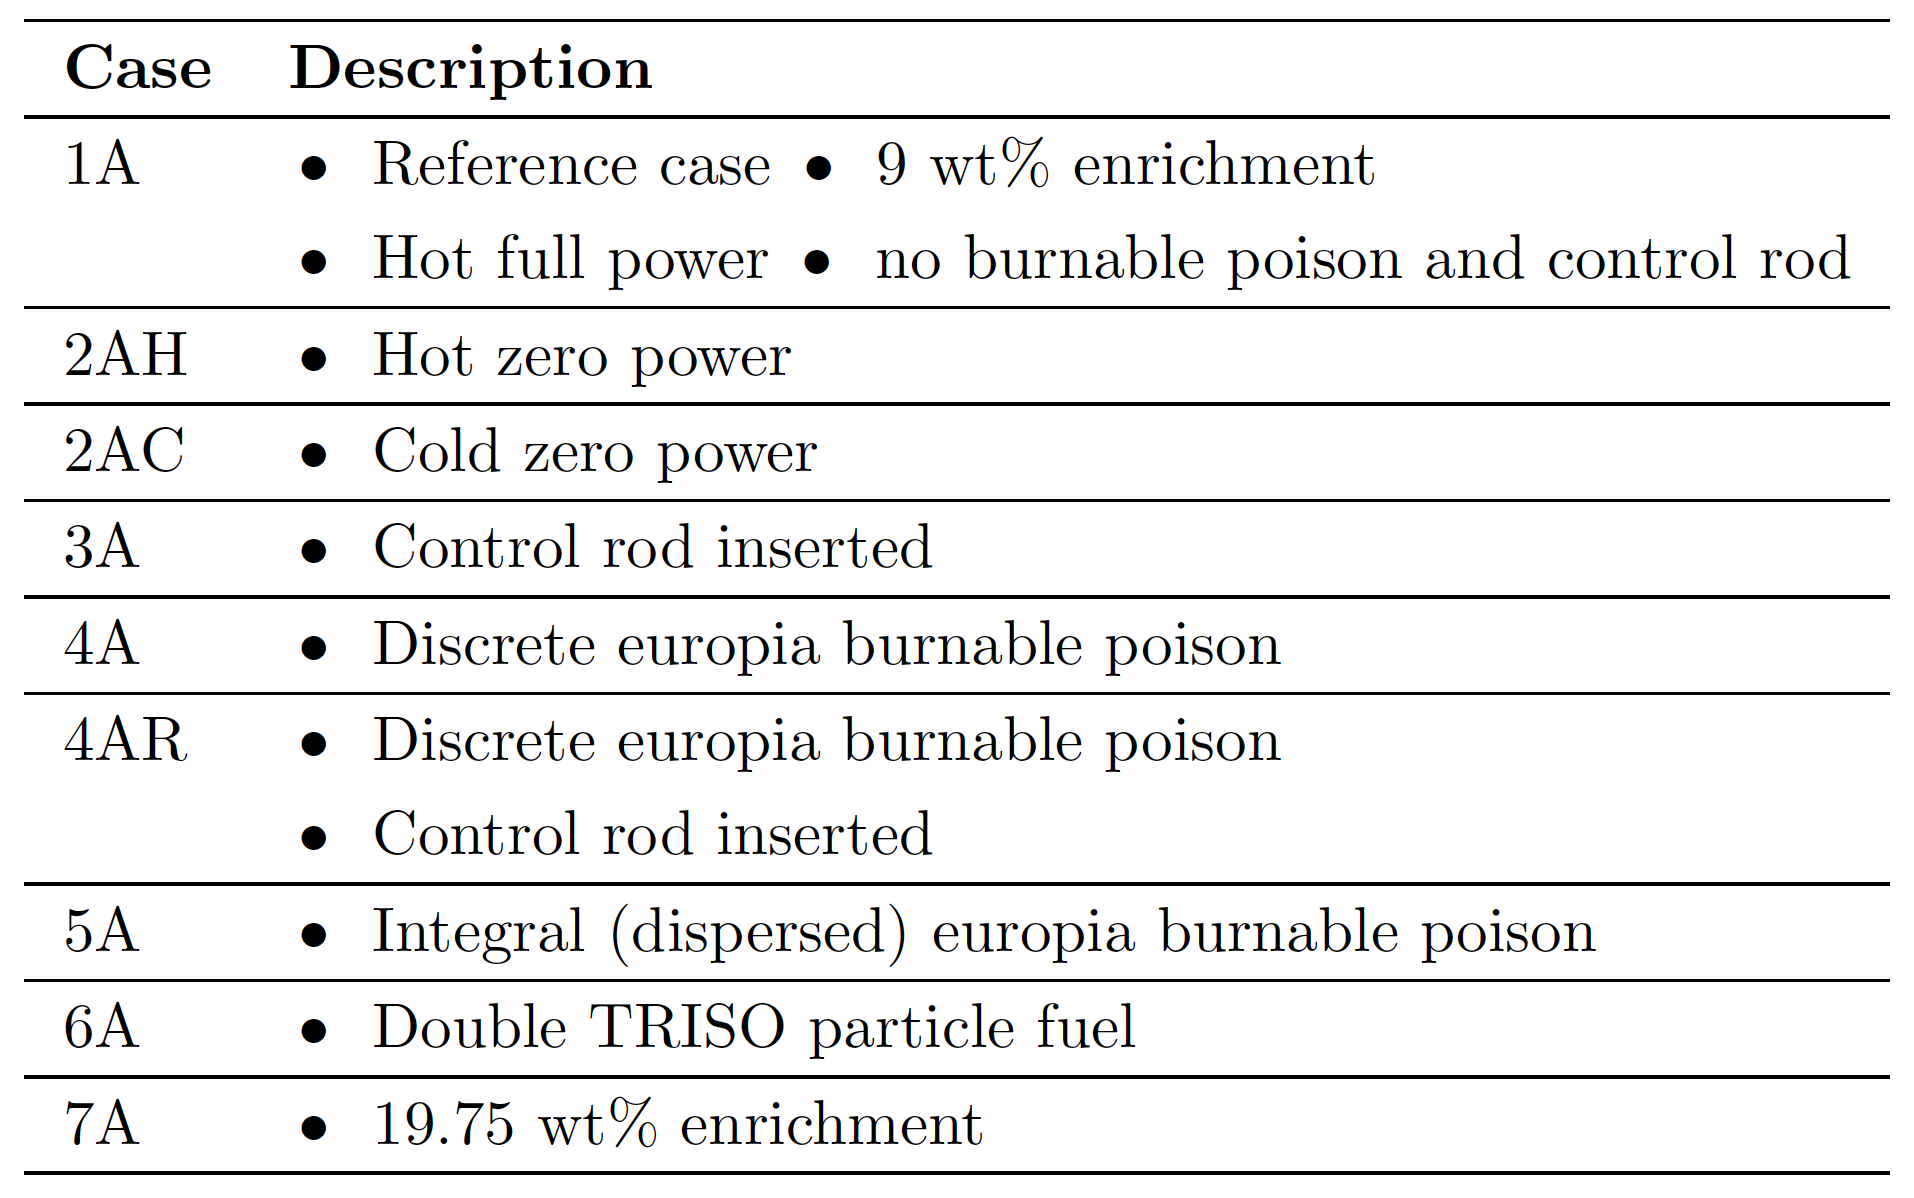
\includegraphics[width=0.6\linewidth]{figures/benchmark-cases.png} 
    \end{table}
    Benchmark participants must produce the following results for 
    the 9 cases: $k_{eff}$, reactivity coefficients ($\beta_{eff}$, 
    $\alpha_D$, $\alpha_{T, FliBe}$, $\alpha_M$), fission source distribution, 
    neutron flux distribution, fuel assembly averaged neutron spectrum
\end{frame}

\subsection*{Key Neutronics Parameters Verification}
\begin{frame}
    \frametitle{AHTR Temp Model $k_{eff}$ and Reactivity Coefficients Verification}
        \begin{table}
            \caption{$k_{eff}$ and reactivity comparison.}
            \vspace{-0.2cm}
            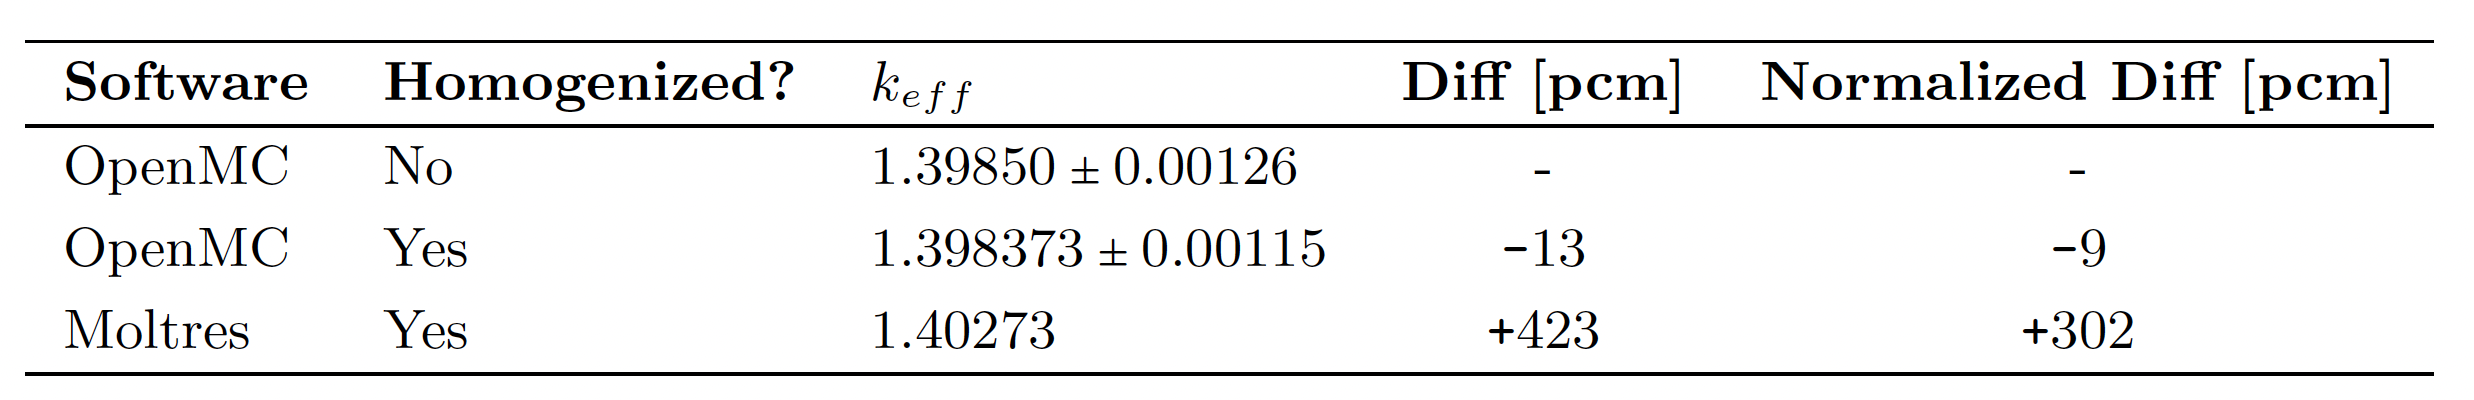
\includegraphics[width=0.9\linewidth]{figures/benchmark-keff.png}
        \end{table}
        The 13pcm $k_{eff}$ and 6pcm reactivity diff, between
        continuous and homogenized OpenMC simulations are within uncertainty, showing 
        that \textbf{selected spatial homogenizations and energy discretizations are 
        acceptable.}
        The Moltres simulation shows a 423pcm diff in $k_{eff}$ and 216pcm 
        diff in reactivity.
        \begin{table}
            \caption{Reactivity coefficients comparison.}
            \includegraphics[width=0.85\linewidth]{figures/benchmark-coeff.png}
        \end{table}
        \textbf{Good agreement} for Moltres' delayed neutron fraction ($\beta_{eff}$) and 
        temperature reactivity feedback ($\frac{\Delta \rho}{\Delta T}$)
\end{frame}

\begin{frame}
    \frametitle{AHTR Temp Model Flux Verification}
    \begin{columns}
    \begin{column}{0.7\textwidth}
    \begin{figure}[]
        \centering
        \includegraphics[width=\linewidth]{figures/benchmark-flux.png} 
        \caption{4-group flux distribution comparison.}
    \end{figure}
    \end{column}
    \begin{column}{0.3\textwidth}
        2-norm Diff [\%]
        \begin{itemize}
            \item Group 1: 0.13\% 
            \item Group 2: 0.08\% 
            \item Group 3: 0.10\% 
            \item Group 4: 0.09\%
        \end{itemize}
        Max Diff [\%]
        \begin{itemize}
            \item Group 1: -10.57\% 
            \item Group 2: +7.58\% 
            \item Group 3: +8.96\% 
            \item Group 4: +6.97\%
        \end{itemize}
    \end{column}
    \end{columns}
\end{frame}

\begin{frame}
    \frametitle{AHTR Temp Model Neutron Energy Spectrum Verification}
            \begin{figure}[]
                \centering
                \includegraphics[width=0.75\linewidth]{figures/benchmark-spectrum.png} 
                \caption{Neutron Energy Spectrum Comparison.}
            \end{figure}
        \textbf{Good agreement} between OpenMC and Moltres models 4-group spectrums.
\end{frame}

\subsection{TRISO Particle Homogenization}
\begin{frame}
    \frametitle{TRISO Particle Homogenization}
    \begin{table}
        \caption{Straightened \acrfull{AHTR} fuel plank $k_{eff}$ for the case with 
        no \gls{TRISO} homogenization and case with homogenization of the four outer 
        layers. Both simulations were run on one BlueWaters supercomputer XE Node 
        using OpenMC with 80 active 
        cycles, 20 inactive cycles, and 8000 particles.}
        \includegraphics[width=0.75\linewidth]{figures/triso-homogenization.png} 
    \end{table}

    The \gls{TRISO} particle outer four-layer homogenization resulted in a $30\%$ 
    speed-up without compromising accuracy with $k_{eff}$ values within each 
    other's uncertainty.

    As a result, the homogenized models are used for all subsequent optimization efforts. 

\end{frame}

\subsection{ROLLO Verification}
\begin{frame}
    \frametitle{ROLLO Successfully Verified with $^{239}Pu$ Critical Bare Sphere}
    \begin{figure}
        \includegraphics[width=0.85\linewidth]{../docs/figures/radius-convergence.png} 
        \caption{Results for each generation for \gls{ROLLO}'s genetic algorithm 
        optimization to the find the critical radius of a  $^{239}Pu$ bare sphere.}
    \end{figure}
    \vspace{-0.2cm}
    \textbf{ROLLO successfully finds the critical radius of the $^{239}Pu$ bare sphere 
    to be 4.9856cm.}
\end{frame}

\begin{frame}
    \frametitle{ROLLO $^{239}Pu$ Critical Bare Sphere Input File}
    \begin{figure}
        \includegraphics[width=0.49\linewidth]{figures/rollo-verify-file.png} 
        \includegraphics[width=0.49\linewidth]{figures/rollo-verify-file2.png}
        \caption{ROLLO $^{239}Pu$ Critical Bare Sphere Input File.}
    \end{figure}
\end{frame}

\begin{frame}
    \frametitle{AHTR Plank Geometry}
    A sine distribution governs TRISO packing fraction distribution: 
    \begin{align}
        \rho_{TRISO}(\vec{x}) &= \left(\textbf{a}\cdot sin(\textbf{b}\cdot x + \textbf{c}) + 2\right) \cdot NF \nonumber
    \end{align}
    \begin{figure}
        \includegraphics[width=0.9\linewidth]{../docs/figures/straightened_plank.png} 
        \caption{Straightened AHTR Plank with 10 fuel cells with random TRISO packing.}
    \end{figure}
    $r_{top}$ and $r_{bot}$ control coolant channel shape: 
    \begin{figure}
        \includegraphics[width=\linewidth]{../docs/figures/coolant-channel-shape.png} 
        \caption{AHTR Plank with coolant channel shape variation, $r_{top}$ = 0.2cm and 
        $r_{bot}$ = 0.3cm.}
    \end{figure}
\end{frame}

\begin{frame}
    \frametitle{Simulation a-3b hypervolume}
    \begin{table}
        \caption{Simulation a-3b hypervolume values at each generation.}
        \includegraphics[width=0.4\linewidth]{figures/a-3b-hypervolume.png} 
    \end{table}

    For each optimization simulation, I must balance convergence and computational cost.

    The hypervolume is calculated by finding the volume between the reference point and 
    the objective values of the Pareto front's reactor models (bigger hypervolume = 
    more converged solution).

    I determine if convergence criteria is met by evaluating if the difference between 
    generations' hypervolume values are getting smaller.
\end{frame}

%%--------------------------------%%


\end{document}



